%\documentclass[a4paper, 12pt, oneside, numbered, print, index, custombib, custommargin, chapter]{Classes/PhDThesisPSnPDF}  % chapter mode
\documentclass[a4paper, 12pt, oneside, numbered, print, index, custombib, custommargin]{Classes/PhDThesisPSnPDF} % whole document

% ******************************************************************************
% ****************************** Custom Margin *********************************

% Add `custommargin' in the document class options to use this section
% Set {innerside margin / outerside margin / topmargin / bottom margin}  and
% other page dimensions
\ifsetCustomMargin
  %\RequirePackage[left=37mm,right=30mm,top=35mm,bottom=30mm]{geometry}
  %\RequirePackage[left=40mm,right=25mm,top=35mm,bottom=30mm]{geometry}  %adis
  \RequirePackage[pdftex, paper=a4paper, hmarginratio=1:1, vmarginratio=1:1, scale=0.75, bindingoffset=15mm, bottom=25mm]{geometry}  %adis
  \setFancyHdr % To apply fancy header after geometry package is loaded %adis: this is needed to draw a hline top of the page
\fi

% *****************************************************************************
% ******************* Fonts (like different typewriter fonts etc.)*************

% Add `customfont' in the document class option to use this section

\ifsetCustomFont
  % Set your custom font here and use `customfont' in options. Leave empty to
  % load computer modern font (default LaTeX font).
  %\RequirePackage{helvet}

  % For use with XeLaTeX
  %  \setmainfont[
  %    Path              = ./libertine/opentype/,
  %    Extension         = .otf,
  %    UprightFont = LinLibertine_R,
  %    BoldFont = LinLibertine_RZ, % Linux Libertine O Regular Semibold
  %    ItalicFont = LinLibertine_RI,
  %    BoldItalicFont = LinLibertine_RZI, % Linux Libertine O Regular Semibold Italic
  %  ]
  %  {libertine}
  %  % load font from system font
  %  \newfontfamily\libertinesystemfont{Linux Libertine O}
\fi

% *****************************************************************************
% **************************** Custom Packages ********************************

% ************************* Algorithms and Pseudocode **************************

%\usepackage{algpseudocode}


% ********************Captions and Hyperreferencing / URL **********************

% Captions: This makes captions of figures use a boldfaced small font.
%\RequirePackage[small,bf]{caption}

\RequirePackage[labelsep=space,tableposition=top]{caption}
\renewcommand{\figurename}{Fig.} %to support older versions of captions.sty


% *************************** Graphics and figures *****************************

%\usepackage{rotating}
%\usepackage{wrapfig}

% Uncomment the following two lines to force Latex to place the figure.
% Use [H] when including graphics. Note 'H' instead of 'h'
\usepackage{float}  	%adis
\restylefloat{figure}	%adis

% Subcaption package is also available in the sty folder you can use that by
% uncommenting the following line
% This is for people stuck with older versions of texlive
%\usepackage{sty/caption/subcaption}
\usepackage{subcaption}

% ********************************** Tables ************************************
\usepackage{booktabs} % For professional looking tables
\usepackage{multirow}

%\usepackage{multicol}
%\usepackage{longtable}
%\usepackage{tabularx}


% *********************************** SI Units *********************************
\usepackage{siunitx} % use this package module for SI units


% ******************************* Line Spacing *********************************

% Choose linespacing as appropriate. Default is one-half line spacing as per the
% University guidelines

% \doublespacing
% \onehalfspacing
% \singlespacing


% ************************ Formatting / Footnote *******************************

% Don't break enumeration (etc.) across pages in an ugly manner (default 10000)
%\clubpenalty=500
%\widowpenalty=500

%\usepackage[perpage]{footmisc} %Range of footnote options


% *****************************************************************************
% *************************** Bibliography  and References ********************

%\usepackage{cleveref} %Referencing without need to explicitly state fig /table

%% Add `custombib' in the document class option to use this section
\ifuseCustomBib

% adis
%\RequirePackage[square, sort, numbers, authoryear]{natbib} % CustomBib

% If you would like to use biblatex for your reference management, as opposed to the default `natbibpackage` pass the option `custombib` in the document class. Comment out the previous line to make sure you don't load the natbib package. Uncomment the following lines and specify the location of references.bib file

% adis
%\RequirePackage[backend=biber, style=numeric-comp, citestyle=numeric, sorting=nty, natbib=true]{biblatex}
\RequirePackage[backend=biber, style=numeric-comp, citestyle=numeric, sorting=nty, natbib=true]{biblatex}
\bibliography{references} %Location of references.bib only for biblatex

\fi

% changes the default name `Bibliography` -> `References'
\renewcommand{\bibname}{References}


% ******************************** Roman Pages *********************************
% The romanpages environment set the page numbering to lowercase roman one
% for the contents and figures lists. It also resets
% page-numbering for the remainder of the dissertation (arabic, starting at 1).

\newenvironment{romanpages}{
  \setcounter{page}{1}
  \renewcommand{\thepage}{\roman{page}}}
{\newpage\renewcommand{\thepage}{\arabic{page}}}


% ******************************************************************************
% ************************* User Defined Commands ******************************
% ******************************************************************************

% *********** To change the name of Table of Contents / LOF and LOT ************

%\renewcommand{\contentsname}{My Table of Contents}
%\renewcommand{\listfigurename}{My List of Figures}
%\renewcommand{\listtablename}{My List of Tables}


% ********************** TOC depth and numbering depth *************************

\setcounter{secnumdepth}{5} %adis{2}
\setcounter{tocdepth}{5}


% ******************************* Nomenclature *********************************

% To change the name of the Nomenclature section, uncomment the following line

\renewcommand{\nomname}{List of Abbreviations}


% ********************************* Appendix ***********************************

% The default value of both \appendixtocname and \appendixpagename is `Appendices'. These names can all be changed via:

%\renewcommand{\appendixtocname}{List of appendices}
%\renewcommand{\appendixname}{Appndx}

% *********************** Configure Draft Mode **********************************

% Uncomment to disable figures in `draftmode'
%\setkeys{Gin}{draft=true}  % set draft to false to enable figures in `draft'

% These options are active only during the draft mode
% Default text is "Draft"
%\SetDraftText{DRAFT}

% Default Watermark location is top. Location (top/bottom)
%\SetDraftWMPosition{bottom}

% Draft Version - default is v1.0
%\SetDraftVersion{v1.1}

% Draft Text grayscale value (should be between 0-black and 1-white)
% Default value is 0.75
%\SetDraftGrayScale{0.8}


% ******************************** Todo Notes **********************************
%% Uncomment the following lines to have todonotes.

%\ifsetDraft
%	\usepackage[colorinlistoftodos]{todonotes}
%	\newcommand{\mynote}[1]{\todo[author=kks32,size=\small,inline,color=green!40]{#1}}
%\else
%	\newcommand{\mynote}[1]{}
%	\newcommand{\listoftodos}{}
%\fi

% Example todo: \mynote{Hey! I have a note}



% ************************* adis **********************************
% \usepackage[linktoc=all]{hyperref}
\usepackage{tabto}
% ************************ Thesis Information & Meta-data **********************
%% The title of the thesis
%\title{Cognitive Radio Communication Framework for Wireless Sensor Networks}#
\title{A Framework for
Adaptive Ride-Sharing and Management
of Electric Vehicles}

%% The full name of the author
\author{Avinash Nagarajan}

%% Department (eg. Department of Engineering, Maths, Physics)
\dept{Department of Computer Science}

%% Supervisors
\supervisors{Dr. Ignacio Casti\~{n}eiras}{Dr. Alan McGibney} {Dr. Pio Fenton}

%% University and Crest
%\university{Cork Institute of Technology}
\university{Munster Technological University}

% Crest minimum should be 30mm.
%\crest{
\includegraphics[width=0.5\textwidth]{CIT_CREST-PANTONE}}
\crest{
\includegraphics[width=0.90\textwidth]{MTU_Logo_Colour_CMYK}}

%\renewcommand{\submissiontext}{change the default text here if needed}

%% Full title of the Degree
\degreetitle{Doctor of Philosophy}

%% College affiliation (optional)
%\college{Cork Institute of Technology}
\college{Munster Technological University}

%% Submission date
% Default is set as 
\degreedate{$8^{th}$ July 2025} 

%% Meta information
%\subject{Electrical \& Electronic Engineering} \keywords{{Low-power wireless networks, receiver-initiated communication, models, interference, measurements} {PhD Thesis} {Engineering} {Cork Institute of Technology}}
\subject{Electrical \& Electronic Engineering} \keywords{{Low-power wireless networks, receiver-initiated communication, models, interference, measurements} {PhD Thesis} {Engineering} {Munster Technological University}}


\ifdefineAbstract
 \pagestyle{empty}
 \includeonly{declaration, abstract}
\fi

% ***************************** Chapter Mode ***********************************
% The chapter mode allows user to only print particular chapters with references
% Title, Contents, Frontmatter are disabled by default
% Useful option to review a particular chapter or to send it to supervisior.
% To use choose `chapter' option in the document class

\ifdefineChapter
	\pagestyle{empty}
 	\includeonly{
 		%dedication,
 		%declaration,
 		acknowledgement,
 		abstract, 
 		chapter1,
 		chapter2,
 		chapter3,
 		chapter4,
 		chapter5,
 		chapter6,
 	}
\fi


% ******************************************************************************
%%%%% Additional packages
\usepackage{mathtools}%phantom minus in matrix
\usepackage{url}
\usepackage{xspace}
\usepackage{siunitx}
\usepackage{graphicx}
\usepackage{caption}
\usepackage{subcaption}
\usepackage{multirow}
\usepackage{multicol}
\usepackage{stackengine}
\usepackage{wrapfig}
\usepackage{textcase}
\usepackage{ifthen}
\usepackage{cases}
\usepackage{amsmath} % For multline equations
\usepackage{amsfonts}
\usepackage{paralist}
\usepackage{booktabs}
\usepackage{makecell}
\usepackage{xspace}
\setlength{\marginparwidth}{2cm} \usepackage{todonotes}
\usepackage{array}
\usepackage{balance}
\usepackage[export]{adjustbox}
\usepackage[inline]{enumitem}
\usepackage{soul}
\usepackage{rotating}
\usepackage{amsthm}
\newtheorem{definition}{Definition}
%\usepackage{showframe}
%\usepackage{layouts}
\usepackage{pdfpages}
\usepackage{acronym}
\usepackage{nomencl}
\usepackage{lscape}
\usepackage{longtable}
\usepackage{algorithm}
\usepackage{tabularx}
\usepackage[noend]{algpseudocode}
\usepackage{listings}
\usepackage{color}
\usepackage{minted}
\usepackage{adjustbox}
\usepackage{outlines}
\usepackage{tikz}
\usepackage{amssymb}
\usepackage{epsfig}
\usepackage{algorithmicx}
\usepackage{geometry}
\geometry{margin=1in}
\usepackage{textcomp}
\usepackage{pgfplots}
\usepackage{hyperref}

\newcommand{\pluseq}{\mathrel{+}=} % Define the \pluseq symbol for aggregation
\def\checkmark{\tikz\fill[scale=0.4](0,.35) -- (.25,0) -- (1,.7) -- (.25,.15) -- cycle;} 
%\definecolor{dkgreen}{rgb}{0,0.6,0}
%\definecolor{gray}{rgb}{0.5,0.5,0.5}
%\definecolor{mauve}{rgb}{0.58,0,0.82}
\definecolor{dkgreen}{rgb}{0, 0, 0}
\definecolor{gray}{rgb}{0, 0, 0}
\definecolor{mauve}{rgb}{0, 0, 0}
\definecolor{blue}{rgb}{0, 0, 0}


\lstset{frame=tb,
  language=Java,
  aboveskip=3mm,
  belowskip=3mm,
  showstringspaces=false,
  columns=flexible,
  basicstyle={\small\ttfamily},
  numbers=left,
  numberstyle=\tiny\color{gray},
  keywordstyle=\color{blue},
  commentstyle=\color{dkgreen},
  stringstyle=\color{mauve},
  breaklines=true,
  breakatwhitespace=true,
  tabsize=3
}

% ******************************************************************************
%%%%% New commands
\newcommand{\fakeparagraph}[1]{\vspace{1mm}\noindent\textbf{#1.}}
\newcommand{\vect}[1]{\boldsymbol{#1}}
\newcommand{\tabvspc}[1]{\parbox{0pt}{\rule{0pt}{#1ex+\baselineskip}}}
\newcommand{\rssi}{\ensuremath{\mathit{RSSI}}\xspace}
\newcommand{\pdr}{\ensuremath{\mathit{PDR}}\xspace}
\newcommand{\ema}{\ensuremath{\mathit{EMA}}\xspace}
\newcommand{\dutycycle}{\textit{duty-cycle}\xspace}
\newcommand{\plr}{\ensuremath{\mathit{PLR}}\xspace}
\newcommand{\fpr}{\ensuremath{\mathit{FPR}}\xspace}
\newcommand{\tpr}{\ensuremath{\mathit{TPR}}\xspace}
\newcommand{\wrt}{w.r.t.\ }
\renewcommand\theadfont{\bfseries}
\newcommand{\home}{\textsc{home}\xspace}
\newcommand{\office}{\textsc{office}\xspace}
\newcommand{\first}{\textsc{first}\xspace}
\newcommand{\second}{\textsc{second}\xspace}
\newcommand{\third}{\textsc{third}\xspace}
\newcommand{\proposedmac}{LUCID\xspace}  %% Name of the proposed MAC protocol
\newcommand{\RNum}[1]{\uppercase\expandafter{\romannumeral #1\relax}}
\newcommand{\tps}{\ensuremath{\mathit{TPS}}\xspace}


%Algo
\algnewcommand\algorithmicforeach{\textbf{for each}}
\algdef{S}[FOR]{ForEach}[1]{\algorithmicforeach\ #1\ \algorithmicdo}

\newcolumntype{L}[1]{>
{\raggedleft\arraybackslash}p{#1}}
\newcolumntype{C}[1]{>{\centering\arraybackslash}p{#1}}
\newcolumntype{R}[1]{>{\raggedright\arraybackslash}p{#1}}

\newcommand{\ie}{i.e.,\ }
\newcommand{\eg}{e.g.,\ }
\newcommand{\vs}{vs.\ }
\newcommand{\free}{\textsc{free}\xspace}
\newcommand{\busy}{\textsc{busy}\xspace}

\newcommand{\thtbns}{\ensuremath{TH_\mathit{TBNS}}\xspace}
\newcommand{\thcount}{\ensuremath{TH_\mathit{count}}\xspace}  

\def\keywords{\vspace{2cm}
{\noindent\textbf{Keywords\\}\,\relax
}}
\def\endkeywords{\par}

% ******************************************************************************
%%%%% When submitting
\newboolean{SUBMIT}
\newboolean{authnotes}

%%%%%-------------------
\setboolean{SUBMIT}{true} %%%% adis: check here
%%%%%-------------------

\ifthenelse{\boolean{SUBMIT}}
{
\setboolean{authnotes}{false}
}{
\setboolean{authnotes}{true}
}

%%%%% For author notes
\ifthenelse{\boolean{authnotes}}
{
%%%%% if the boolean authnotes is true define the macros AND print a diagonal
%%%%% draft watermark, to remember they are in
\newcommand{\ram}[1]{\footnote{{\bf avinash: #1}}}
\newcommand{\adis}[1]{\footnote{{\bf nacho: #1}}}
\newcommand{\dirk}[1]{\footnote{{\bf Alan: #1}}}
\usepackage{draftwatermark}
\SetWatermarkLightness{0.85}
}{
%%%%% otherwise, just define the macros to avoid compilation errors, but ignore
%%%%% the content of the notes 
\newcommand{\avinash}[1]{}
\newcommand{\nacho}[1]{}
\newcommand{\alan}[1]{}
\newcommand{\pio}[1]{}


}


% ******************************************************************************
\begin{document}

\frontmatter

\begin{titlepage}
  \maketitle
\end{titlepage}
% ******************************* Thesis Declaration ***************************

\begin{declaration}

This dissertation is entirely the candidate's own work except where otherwise accredited and has not been submitted for an award at any other institution. \\

\noindent
The research presented in this thesis was carried out in compliance with the MTU Code of Good Practice in Research. 

% Remainder will be inserted by the class file. 



%I hereby declare that this submission is my own work and that, to the best of my knowledge and belief, it contains no material previously published or written by another person nor material to a substantial extent has been accepted for the award of any other degree or diploma of the university of higher learning, except where due acknowledgement has been made in the text. 

% Author and date will be inserted automatically from thesis.tex \author \degreedate

\end{declaration}
% ******************************* Thesis Dedidcation ********************************

\begin{dedication} 

\begin{minipage}[t]{\textwidth}
\begin{flushright}
\textit{To my mother and father for everything}\\
%\textit{මගේ පවුල වෙත පුදමි}
\end{flushright}
\end{minipage}

\end{dedication}

% ************************** Thesis Acknowledgements **************************

\def\mydate{\leavevmode\hbox{\twodigits\day.\twodigits\month.\the\year}}
\def\twodigits#1{\ifnum#1<10 0\fi\the#1}

\begin{acknowledgements}
First and foremost, I extend my deepest gratitude to my supervisors Nacho, Alan and Pio for their unwavering guidance and support throughout this journey. In particular, I would like to thank Nacho for going above and beyond in supporting me during the most challenging times of the COVID-19 pandemic. His understanding, encouragement, and timely advice were invaluable as I navigated the shift to remote work, battled homesickness, and strove to meet important deadlines.

I am also grateful to my parents and friends, whose love, patience, and steadfast encouragement have kept me motivated over these past years. Thank you for believing in me, for celebrating every milestone, and for putting up with my highs and lows as I pursued this PhD.

Finally, this research would not have been possible without the generous funding provided by Science Foundation Ireland under Grant number 18/CRT/6222. Their support has been instrumental in enabling me to undertake and complete this work.

% I would also like to acknowledge Confirm SmartQC project providing the opportunity to enhance the DLT decision support tool  



\vspace{1cm}
\noindent
\begin{minipage}[t]{\textwidth}
\begin{flushright}
Cork,  \\
Avinash Nagarajan
\end{flushright}
\end{minipage}

\vspace{1cm}
\noindent
\begin{minipage}[t]{\textwidth}
\centering
\rule{0.10\textwidth}{0.4pt}
\end{minipage}
\vspace{1cm}

%The research leading to this doctoral thesis has been funded by the Irish Research Council in collaboration with the then United Technologies Research Centre, Cork, Ireland. The funding was the result of the award ``Enterprise Partnership Scheme Postgraduate Scholarship 2014'' under the project ID EPSPG/2014/66 (Cognitive Radio Communication Framework for Wireless Sensor Networks). 

\end{acknowledgements}

\begin{abstract}
Europe aims for carbon neutrality by 2050, with transportation currently amounting 20\% of
its total emissions. Motivated by the sustained mass transition to Autonomous Electric
Vehicles (AEVs) and by the distributed energy generation and storage of local Smart Energy
Communities (SECs), this thesis presents the design, implementation and evaluation of a
carbon-neutral, community-based, scalable ride-sharing service. Its models formalise the
partition of an AEVs fleet over the SECs of a city, as well as the allocation of trip petitions (TPs) to AEVs, their routing and charging scheduling over a simulated time horizon. These models integrate energy generation, allocation and re-routing constraints to maximise the number of TPs served. The solution approach to implement the models includes the
application of Greedy-based Heuristics and Metaheuristics, Reinforcement Learning and
Mixed Integer Programming techniques. A parameterised instance generator is developed,
aligning existing benchmarks (i.e. Google HashCode) and public datasets (i.e. NYC taxis) to
the proposed problem formulations and testing the service under various configurations.
The ride-sharing service is proven to scale well, when applied to very large instances,
providing fast and competitive results. Overall, this thesis contributes to green
transportation by providing a computational efficient, scalable, and environmentally
sustainable ride-sharing service.

% \keywords{ Trust}

\end{abstract}
 
% 

\begin{minipage}[t]{\textwidth}

\chapter*{\centering \Large List of Publications}

\begin{enumerate}

    \item \textbf{Nagarajan, A.}; McGibney, A.; Fenton, P. and Castiñeiras, I. (2023). A Carbon-Neutral, Community-Based, Reactive and Scalable Ride-Sharing Service.  In Proceedings of the 12th International Conference on Smart Cities and Green ICT Systems.

\end{enumerate}

\end{minipage}




\tableofcontents
\listoffigures
\listoftables

% \printnomenclature[space] space can be set as 2em between symbol and description
% \printnomenclature[3em]

\newpage
\markboth{}{List of Abbreviations}
\addcontentsline{toc}{chapter}{List of Abbreviations}
\printnomenclature

\chapter*{List of Abbreviations}
\label{acronyms}

\begin{acronym}
    \acro{AEV}     Autonomous Electric Vehicle  
    \acro{ALNS}    Adaptive Large Neighbourhood Search  
    \acro{AMoD}     Autonomous Mobility-on-Demand  
    \acro{AV}      Autonomous Vehicle  
    \acro{BA-DA}   Hybrid Bees Algorithm with Deterministic Annealing  
    \acro{BA-SA}   Hybrid Bees Algorithm with Simulated Annealing  
    \acro{cA2C}     Contextual Multi-Agent Actor-Critic  
    \acro{cDQN}     Contextual Deep Q-Learning  
    \acro{CAV}      Connected Autonomous Vehicle  
    \acro{CS}      Charging Station 
    \acro{CTSPAV}   Commute Trip Sharing Problem for Autonomous Vehicles  
    \acro{CTSP}     Commute Trip Sharing Problem  
    \acro{CVRP}    Capacitated Vehicle Routing Problem  
    \acro{DARP}    Dial-a-Ride Problem  
    \acro{DQN}     Deep Q-Network
    \acro{DRL}      Deep Reinforcement Learning  
    \acro{E-VRPTW}  Electric Vehicle Routing Problem with Time Windows  
    \acro{EPSG}    European Petroleum Survey Group (used in coordinate reference systems)  
    \acro{EU}     European Union  
    \acro{FCFS}     First-Come, First-Served      \acro{FIFO}    First-In-First-Out
    \acro{GA}      Genetic Algorithm  
    \acro{GCN}     Graph Convolutional Network
    \acro{GH01}     Google Hashcode Dataset Instance 01
    \acro{GH02}     Google Hashcode Dataset Instance 02
    \acro{GH03}     Google Hashcode Dataset Instance 03
    \acro{GHG}     Greenhouse Gas  
    \acro{GPS}     Global Positioning System  
    \acro{HDARP}   Heterogeneous Dial-a-Ride Problem  
    \acro{HVRP}    Heterogeneous Fleet Vehicle Routing Problem  
    \acro{ITS}     Intelligent Transportation Systems  
    \acro{IT}      Information Technology  
    \acro{LNS}     Large Neighbourhood Search  
    \acro{LS}      Local Search  
    \acro{MIP}     Mixed Integer Programming  
    \acro{MPC}      Model Predictive Control  
    \acro{NY01}     NYC Dataset Instance 01
    \acro{NYC}     New York City  
    \acro{OGC}     Open Geospatial Consortium  
    \acro{PDP}     Pick-up and Delivery Problem  
    \acro{POMDP}    Partially Observable Markov Decision Process 
    \acro{PuP}     Pick-Up Point
    \acro{QGIS}    Quantum Geospatial Information System  
    \acro{RES}     Renewable Energy Sources  
    \acro{RL}      Reinforcement Learning  
    \acro{SAEV}     Shared Autonomous Electric Vehicle  
    \acro{SAMoD}    Shared Autonomous Mobility-on-Demand  
    \acro{SA}      Simulated Annealing  
    \acro{SEC}     Smart Energy Community  
    \acro{TP}     Trip Petition 
    \acro{TSP}     Traveling Salesman Problem  
    \acro{TS}       Tabu Search  
    \acro{UN}     United Nations  
    \acro{V2I}      Vehicle-to-Infrastructure  
    \acro{V2V}      Vehicle-to-Vehicle  
    \acro{VNS}      Variable Neighbourhood Search  
    \acro{VRPTW}   Vehicle Routing Problem with Time Windows  
    \acro{VRP}     Vehicle Routing Problem  
\end{acronym}


% ******************************** Main Matter *********************************
\mainmatter

\chapter{Introduction}
\label{chapter1}
This chapter gives an outline of the important developments and difficulties in the transport
and energy sectors that form the basis for this research. Section \ref{sec:motivation} motivates the work being presented. Then, Section \ref{sec:contributions} enumerates its research objectives and contributions. Next, Section \ref{publications} lists the publications emanating from the research contributions. Finally, Section \ref{structure} discusses the structure of the document. This chapter gives an outline of the important developments and difficulties in the transport and energy sectors that form the basis for this research.

\section{Motivation}
\label{sec:motivation}

% \begin{figure}[htbp]
%     \centering
%     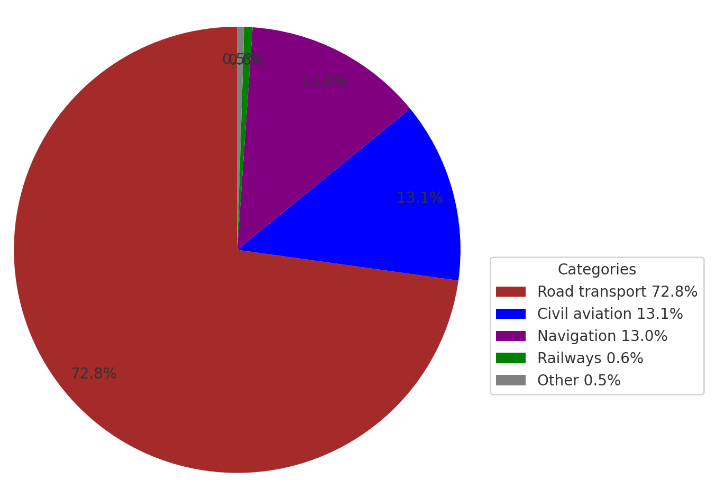
\includegraphics[scale=0.55]{Crest/Images/ghg_stats.png}
%     \caption{Greenhouse gas emissions from transport by mode 2014-20 \cite{alfaseeh2019multi}}
%     \label{fig:ghg_stats}
% \end{figure}
Recent data has shown that between the years 1890 and 2008, the temperature in Ireland. 
has grown by 0.7 degree Celsius. It has changed the growing season, affecting farming, and
has increased the number of animals suited to warmer temperatures. Data trends show an
increase in the frequency and impact of storms in the last few decades \cite{alfaseeh2019multi}. Similar situations are being seen all over the world (such as China, India, Mexico, Brazil just to name a few countries). Indeed, up to 2021, Bhutan is the only carbon-neutral country in the world where the daily operation of the country does not cause lasting damage to the environment \cite{europeancommission2024promoting}. As a way to fight these growing climate threats, the European Union (EU) and the European Commission have presented a package of measures designed to make Europe the first climate-neutral continent in the world by 2050. Some of the critical components of this policy include cutting emissions, preserving the natural environment and investing in cutting edge research and innovation \cite{shariff2022state} . This European Green Deal is the long-term strategy of the EU to protect humans, animals and plants by cutting pollution and securing a healthy planet for generations to come \cite{greendeal}.

The transportation sector has been identified as a key area to undergo significant
transformation as a result of the aforementioned Green Deal. In the last decade there has
been growing awareness about the hazardous effects of logistic activities, such as
transportation, which has a considerable impact on the ecological environment, and
therefore requests for more environmentally friendly practices. The EU has targeted a 40\%
reduction in Green House Gas (GHG) emissions by 2030 with respect to the levels of 1990
\cite{europeancommission2024promoting}. According to the European Environment Agency, this is a challenge for the transportation sector, which is responsible for 20\% of total GHG emissions. Furthermore, according to the 2019 report of the world energy outlook series, the future estimation of energy systems indicates that a severe loss in available amounts of fossil energy will happen by 2040 \cite{greendeal}. Therefore, electrification and autonomy of the transportation systems are viewed as a critical avenue to achieving the ambitions as set-out in the EU Green Deal.

The operation of transportation networks through (increasingly Autonomous) Electric
Vehicles (AEVs) fleets requires also a profound change in the energy sector, where the use
of Renewable Energy Sources (RES) must become the norm \cite{alfaseeh2019multi} \cite{baudru2024comparative} and decentralisation enables stability and flexibility of the grid (smart grid). This not only requires specific policies, but a general shift in mindset in terms of how to effectively manage this decentralised generation to effectively service the demands of end users and customers. The generation and availability of RES is volatile by nature and, instead of adapting it to current society demands, an emphasis must be placed on being more cognisant of the efficient use of every unit of energy required. In addition to large-scale wind and solar farms (which are typically managed at a national level), Smart Energy Communities (SECs) are decentralised clusters of energy users—such as households, businesses, or institutions—that are locally interconnected and capable of both generating and consuming RE. Typically supported by digital infrastructure and storage systems, SECs coordinate energy generation (e.g., via solar or wind), storage (e.g., through batteries), and demand within a geographically bounded area. By enabling distributed energy generation, peer-to-peer trading, and cooperative decision-making, SECs contribute to a more resilient, carbon-neutral grid. They represent a foundational model for the emergence of the term ‘Energy Citizen’, empowering individuals and communities to participate actively in the management of the electric power system, and thereby enhancing both its efficiency and sustainability.

In response to these imperatives, several strategies have been proposed, including the
adoption of RES \cite{gradisar2000enhancing}, advancements in vehicle technology [51], and the implementation of Intelligent Transportation Systems (ITS) \cite{wallar2019optimizing}. Within ITS, Ride-sharing has presented new opportunities for the SEC sector to be productive with energy usage \cite{agatz2012optimization}. Dynamic ride-sharing systems aim to match riders and drivers with similar itineraries and time schedules on short-notice \cite{soa_rideshare}. These systems can reduce the number of cars used for personal travel (improving the utilisation of available seat capacity) as well as the total distance for such travels, thus reducing the environmental impact.

Motivated by the aforementioned sustained mass transition to AEVs and by the distributed
energy generation and storage of local SECs, this PhD thesis presents the design, implementation
and evaluation of a carbon-neutral, community-based, scalable ride-sharing system. The
PhD thesis considers a future where a ride-sharing service must rely on a 100\% AEV fleet
operating solely on RES. Emphasis is placed on individual citizens (rather than on haulage
transportation) that collectively aim to minimise their impact on the environment through
the use of ride-sharing commutes powered by green energy sources. The ride-sharing
service entails an AEV fleet operating in a city that encapsulates multiple distributed SECs,
each of them producing RES over a time horizon, owning and operating a number of AEVs and charge stations. Each SEC sets out its available AEVs for ride-sharing based on the RES
energy generation that can be used to charge them.

The challenges to operate such a ride-sharing service include managing how the overall fleet of AEVs is distributed across the various SECs of a city. While each SEC initially deploys its own set of AEVs, the dynamic nature of ride-sharing operations and inter-SEC collaboration often requires a city-wide perspective, where the effective partitioning and reallocation of AEVs between SECs must be carefully coordinated, as well as the allocation of trip petitions (TPs) to AEVs, their routing and charging scheduling over a simulated time horizon. These challenges become even
more pronounced by the need to operate at scale (with large EV fleets across metropolitan
areas), in real-time (with the service processing the TPs as they arise), and under dynamic
resources (with the number of active AEVs depending on RES availability over time across
multiple locations). Finally, the distributed SECs are indeed inter-related, and therefore
enabling decentralised co-operation to optimise their resources.

All in all, the EU Green Deal targets 2050 to be energy-neutral, envisioning a sustained
transition from diesel-based transportation to AEVs, and from a traditional energy market to
a fully RES-based one. To enable this change, the transportation sector must demonstrate
leadership by accelerating the use of AEVs and SECs. This PhD thesis contributes to this vision for green transportation by providing a computational efficient, scalable, and environmentally sustainable ride-sharing service.


% Transportation is a major contributor to environmental degradation, accounting for 28\% of greenhouse gas (GHG) emissions and 20\% of total energy consumption in the United States alone \ref{fig:ghg_stats} \cite{alfaseeh2019multi}. Globally, the sector relies heavily on oil-based fuels, which are not only non-renewable but also highly polluting, exacerbating the climate crisis. The pressing need to reduce these emissions has prompted international frameworks such as the \textit{United Nations Sustainable Development Goals (SDGs)} \cite{shariff2022state} and the \textit{European Green Deal} \cite{europeancommission2024promoting}, which emphasise carbon neutrality as an essential—not optional—objective. The European Green Deal, for instance, aims to make Europe the first climate-neutral continent by 2050, prioritising the decarbonisation of energy-intensive sectors like transportation \cite{greendeal}.

% In response to these imperatives, several strategies have been proposed, including the adoption of RES \cite{gradisar2000enhancing}, advancements in vehicle technology \cite{hajari2021distributed}, and the implementation of \textit{Intelligent Transportation Systems (ITS)}\cite{wallar2019optimizing}. ITS has proven to be especially effective, optimising various transportation operations such as dynamic routing, traffic flow control, and energy-efficient vehicle scheduling\cite{fiedler2018impact}. By enhancing operational efficiency and reducing congestion, ITS significantly curbs fuel consumption and emissions \cite{alfaseeh2019multi} \cite{baudru2024comparative}.

% Recent years have seen a paradigm shift in the transportation sector, marked by the widespread adoption of \textit{electric vehicles (EVs)} and the rise of \textit{ride-sharing services}. While ride-sharing services reduce the number of vehicles on the road, lowering pollution and traffic congestion, integrating EVs into these systems provides further environmental benefits by replacing fossil fuel-based engines with zero-emission alternatives \cite{gradisar2000enhancing}. However, achieving large-scale adoption of EV-based ride-sharing services requires overcoming challenges such as:
% \begin{enumerate}
%     \item \textbf{Passenger-to-vehicle allocation:} Matching passengers to available vehicles in real time while minimising operational costs and maximising passengers served \cite{alonso2017ondemand} \cite{optimiserideshare} \cite{hasan2018community}.
%     \item \textbf{Vehicle routing:} determining the most energy-efficient routes that also account for passenger travel demands \cite{meng2021dynamic} \cite{ghandeharioun2023rideshare}.
%     \item \textbf{EV charging scheduling:} Ensuring efficient charging operations that minimise downtime \cite{song2023electric} \cite{satoya2014community} \cite{Reference104}.
% \end{enumerate}

% These challenges become even more pronounced as the scale of operations increases. Efficient algorithms must not only address the travel demands but also ensure scalability to support the deployment of large EV fleets across metropolitan areas.

% \subsection{Role of Smart Energy Communities (SECs)}

% SECs integrate RES, such as solar and wind, with smart grid technologies, enabling the localised production, distribution, and consumption of clean energy\cite{hildermeier2019smart}. Beyond their potential to reduce reliance on fossil fuels, SECs could be used as a solution to enable EV-based ride-sharing services. Specifically, they enable:
% \begin{itemize}
%     \item \textbf{Dynamic energy allocation:} Matching charging schedules to periods of high renewable energy availability\cite{hemavathi2022study}\cite{vanSummeren2019community}.
%     \item \textbf{Depot functionality:} Serving as depots for ride-sharing EVs.
%     \item \textbf{Collaborative operations:} Negotiating with other SECs to balance resources and maximise the number of trips served\cite{shariff2022state}.
% \end{itemize}

\section{Research Objectives and Contributions}
\label{sec:contributions}
The PhD thesis has the following 3 research objectives:

\subsection{Research Objective 1}
\textbf{A Carbon-Neutral, Community-Based, Reactive and Scalable Ride-Sharing Service.}
This research objective entails the design, implementation and evaluation of a ride-sharing service aligning with the ambition of the aforementioned EU Green Deal goals.

Specifically, the research objective leads to the following research contributions:
\begin{itemize}
    \item \textbf{Contribution 1:} The formulation of a ride-sharing simulation service that explicitly incorporates the conditions outlined above, namely the decentralised structure of SECs, dynamic TPs, RES integration, and the flexible allocation of AEVs, all operating with the goal of maximising TP fulfilment, presented as a variant of the classical Dynamic Vehicle Routing Problem with Time Windows \cite{vrp_survey}. The dynamic resources are provided
    by a number of SECs spread across a city, each of them owning a number of AEVs
    and using its own RES generation function to dynamically charge (and release) them
    over time. The dynamic requests are provided via TPs released over time,
    each of them with its own location and pick-up/drop-off times. The formulation of
    the ride-sharing service integrates energy generation, allocation and reactive re-
    routing constraints, with the objective function of maximising the overall number of
    TPs being served.

    \item \textbf{Contribution 2:} The design and implementation of a ride-sharing service, based on an algorithm following a reactive-based simulation approach on top of a greedy-based decision-making process. The algorithm favours scalability over optimality, therefore evaluating its applicability to real-world instances based on the transportation of large cities.

    \item \textbf{Contribution 3:} The development of a parameterised instance generator to align existing benchmarks (i.e. Google HashCode) and public datasets (i.e. NYC taxis) to the proposed problem formulation of Contribution 1. This is paired with the generation
    of a problem-specific benchmark for testing the performance of the solution approach of Contribution 2 under various configurations.     
\end{itemize}

\subsection{Research Objective 2}
\textbf{Decentralised Vehicle Allocation for Community-Based Ride-Sharing Services.}
This research objective extends Research Objective 1 by integrating the design,
implementation and evaluation of the vehicle fleet allocation to the ride-sharing service.

Specifically, the research objective leads to the following research contributions:
\begin{itemize}
    \item \textbf{Contribution 4:} The formulation of the vehicle allocation problem both as a centralised optimisation problem (using a MIP formulation) and as a decentralised one, using an iterative negotiation process among connected-SECs. On the latter, each SEC acts as an independent agent, and carries out a number of negotiations with any other SEC it is connected to over a simulated time horizon. In such negotiations, connected
    communities decide the potential exchange of AEVs among them, based solely on their local information. The criticality of the vehicle allocation problem lies on its co-
    operation with its underlying ride-sharing problem to ensure adequate AEV to TP
    matching and routing. Once a SEC allocated a fixed number of AEVs from the AEV
    fleet, it manages the TPs of its own neighbours by operating the ride-
    sharing solution approach of Contribution 2.

    \item \textbf{Contribution 5:} The implementation of the vehicle allocation problem, using a novel Multi-Objective and Multi-Agent Reinforcement Learning (RL) algorithm, involving Deep Q-Learning with Graph Convolutional Networks. The algorithm equips SECs with the ability to learn from previous-negotiations, enabling them to improve their decision-making as the simulated time horizon goes by.

    \item \textbf{Contribution 6:} The modification of the instance generator and problem benchmark of Contribution 3, for it to align to the problem formulation of Contribution 4, as well as its further measuring of the solution approach of Contribution 5 under different community connectivity-levels and transport request distributions.    
\end{itemize}

\subsection{Research Objective 3}
\textbf{Reward-based Charging Schedule for a Community-based Ride-sharing Service.}
This research objective extends Research Objective 1 by integrating the design,
implementation and evaluation of reward-based charging scheduling to the ride-sharing
service.

Specifically, the research objective leads to the following research contributions:
\begin{itemize}
    \item \textbf{Contribution 7:} The formulation of the reward-based charging schedule, where each SEC owns a number of Charging Stations (CSs), and its RES generated being split into (i) the energy used to release its own AEVs and (ii) the energy used to recharge already operative AEVs. The charging schedule exploits the inter-relation of SECs, enabling (1) host TPs to be served by an AEV of a different SEC, and (2) such AEVs to recharge their batteries in a host CSs in return.

    \item \textbf{Contribution 8:} The implementation of the reward-based charging schedule via a decision-making process accounting for different factors, including the proximity and waiting times of available CSs, the potential for service interruptions due to charging, and the dynamic re-allocation of AEVs based on real-time assessments of energy
    consumption and vehicle availability. Additionally, the algorithm incorporates the
    flexibility to modify charging schedules dynamically by considering the collective
    prospects of multiple AEVs.

    \item \textbf{Contribution 9:} The modification of the instance generator and problem benchmark of Contribution 3, for it to align to the problem formulation of Contribution 7, as well as its further measuring of the solution approach of Contribution 8 under various configurations.    
\end{itemize}

% \subsection{Contributions}
% This thesis makes the following key contributions:

% \begin{enumerate}
%     \item \textbf{A carbon-neutral, community-based, reactive, and scalable ride-sharing service tailored to SECs.} 
%     This service consists of a network of independent but interrelated SECs, each equipped with its own EVs and Trips Petitions(TPs). These SECs operate autonomously but are capable of collaborating with one another to maximise the number of trips served. It is built on an algorithmic framework for real-time vehicle allocation and routing, enabling dynamic responses to evolving transportation demands.
    
%     The scalability of the system is a key feature, supported by a parameterised instance generator that aligns with existing benchmarks such as Google HashCode and public datasets like the NYC taxi data. This generator enables the evaluation of the system across diverse operational configurations, such as variations in trip flexibility, fleet size, and community connectivity. The solution was shown to process up to 10,000 trip petitions in less than two minutes, demonstrating its capability to handle large-scale urban ride-sharing scenarios.
    
%     Real-world evaluations using the NYC taxi dataset revealed that the system reduced the number of vehicles required by 84\% compared to traditional private transport, significantly decreasing traffic and pollution. The additional travel distance incurred due to ride-sharing was reasonably small, at only 21\%. This result indicates that the proposed method achieves a good balance between minimising vehicle usage and ensuring reasonable travel times, making it well-suited for large-scale urban mobility systems.
    
%     \item \textbf{A decentralised vehicle allocation framework for community-based ride-sharing services.} 
%     In this framework, multiple independent SECs within a metropolitan area manage their transportation needs by competing for vehicle resources to serve TPs. The vehicle allocation problem is modelled using centralised and decentralised approaches to examine how varying levels of community connectivity—defined as the degree of communication and resource sharing between SECs—affect resource distribution and operational performance.
    
%     To solve this complex allocation challenge, a Multi-Objective and Multi-Agent Reinforcement Learning (RL) method was developed. This approach combines Deep Q-Learning with Graph Convolutional Networks (GCNs), enabling SECs to negotiate vehicle allocations based on historical performance and current operational needs. The decentralised structure allows SECs to make independent decisions while collaboratively optimising overall system performance. This approach directly builds on the foundational allocation and routing algorithm described in Contribution 1.
    
%     The framework was evaluated using public datasets, including NYC taxi data and Google HashCode, and demonstrated scalability for large instances with up to 10,000 trips processed in a few seconds. The results show that the framework efficiently distributes vehicles across SECs, leading to higher operational efficiency, as reflected in the increased number of trip petitions served in real-time.

%     \item \textbf{An intelligent charging scheduler for a proactive, community-based, carbon-neutral ride-sharing service.} 
%     Building on the allocation and routing algorithm from Contribution 1, this scheduler optimises the charging processes for EVs within the SECs while ensuring carbon neutrality through the exclusive use of renewable energy. The scheduler addresses critical operational challenges, including minimising EV downtime and ensuring sufficient availability of vehicles for ride-sharing operations.
    
%     The scheduler incorporates a proactive approach to align charging activities with renewable energy production and travel demand. This approach allows SECs to manage their EV fleets efficiently, reducing the impact of charging on TPs fulfilled and operational reliability. The results demonstrate that the scheduler significantly enhances fleet efficiency, as reflected by a higher number of trip petitions served while maintaining carbon-neutral operations.
    
%     Evaluations using public datasets, such as NYC taxi data and Google HashCode, confirmed the solution’s scalability and adaptability to real-world conditions. The scheduler balances frequent charging needs with travel demands. This contribution extends the framework’s applicability to large-scale urban systems by enabling integration of EV charging into the overall ride-sharing service.
    
% \end{enumerate}

\section{Publications}
\label{publications}
The PhD thesis has the following 3 publications:
\begin{enumerate}
    \item \textbf{Publication 1 - Research Objective 1: 
        A Carbon-Neutral, Community-Based, Reactive and Scalable Ride-Sharing Service.} \cite{smartgreens}.
         \begin{itemize}
             \item Authors: Nagarajan, A.; McGibney, A.; Fenton, P. and Castiñeiras, I.
             \item Venue: In Proceedings of the 12th International Conference on Smart
                   Cities and Green ICT Systems.
             \item Year: 2023.
             \item Link: \href{https://www.scitepress.org/PublicationsDetail.aspx?ID=tZN50XMYOaQ=&amp;t=1}{SCITEPRESS publication link}
             \item Acceptance Rate: 30\% for full-paper publications.
             \item Github: \ \url{https://github.com/Nasheor/reactive\_rideshare}   
         \end{itemize}

    \item \textbf{Publication 2 - Research Objective 2:
    Decentralised Vehicle Allocation for Community-Based Ride-Sharing Services} \cite{nagarajan2024decentralised}.
         \begin{itemize}
             \item Authors: Nagarajan, A.; McGibney, A.; Fenton, P. and Castiñeiras, I.
             \item Venue: Communications in Computer and Information Science (Volume 1989).
             \item Year: 2024.
             \item Link: \href{https://link.springer.com/chapter/10.1007/978-3-031-70966-1_2}{Springer publication link}
             \item Acceptance Rate: 33\% for full-paper publications.
             \item Note: The publication requested a 30\% of novelty with respect to Publication 1. Indeed, a 70\% of novelty is provided in the paper.
             \item Github:\ \url{https://github.com/Nasheor/Fleet_allocation}   
         \end{itemize}

    \item \textbf{Publication 3 - Research Objective 3:
    Reward-based Charging Schedule for a Community-based Ride-sharing Service.} \cite{rewardcharging}.
         \begin{itemize}
             \item Authors: Nagarajan, A.; McGibney, A.; Fenton, P. and Castiñeiras, I.
             \item Venue: In Proceedings of the 3rd International Conference on IEEE Smart Mobility.
             \item Year: 2024.
             \item Link: \href{https://ieeexplore.ieee.org/document/10733393}{IEEE publication link}
             \item Acceptance Rate: 51\% for full-paper publications.
             \item Note: The publication requested a 30\% of novelty with respect to Publication 1. Indeed, a 70\% of novelty is provided in the paper.
             \item Github:\ \url{https://github.com/Nasheor/EcoRideSchedule}   
         \end{itemize}
\end{enumerate} 

\section{Structure}
\label{structure}
The remainder of this PhD thesis is organised as follows:
\begin{itemize}
    \item Chapter \ref{chapter2} presents an analysis of the current body of work that serves as the foundation for the PhD thesis.

    \item Chapter \ref{chapter3} presents the research objective 1, with the design, implementation and evaluation of a ride-sharing service aligning with the ambition of the aforementioned EU Green Deal goals.

    \item Chapter \ref{chapter4} presents the research objective 2, with the design, implementation and evaluation of the vehicle fleet allocation integrated to the ride-sharing service.

    \item Chapter \ref{chapter5} presents the research objective 3, with the design, implementation and evaluation of the reward-based charging scheduling integrated to the ride-sharing service.

    \item Chapter \ref{chapter6} presents a summary of the findings and a discussion of potential future work.
\end{itemize}

\chapter{Background}
\label{chapter2}

I love football \cite{sarmento2014match}

This chapter presents an analysis of the current body of work that serves as the foundation for the PhD thesis on a carbon-neutral dynamic ride-sharing service. It positions the Ride-Sharing problem, its variants and associated challenges, including the optimisation issues connected with ride-sharing, the function of AEVs, the integration of SECs, and the crucial necessity of charging infrastructure. The chapter provides the context for the design, implementation and evaluation of the novel ride-sharing models proposed in subsequent chapters.

\section{The Vehicle Routing Problem (VRP)}
\label{sec:vrp}
This section provides the background necessary to understand the dynamic ride-sharing framework developed in this PhD thesis. Section~\ref{sec:vrp} begins by introducing the classical Vehicle Routing Problem (VRP), outlining its fundamental definitions and common variants. Section~\ref{Section22} then shifts focus to the ride-sharing paradigm, detailing how the VRP can be adapted to transport passengers instead of goods and discussing time-window constraints, routing decisions, and service requirements. Finally, Section~\ref{sec:dynamic} explores the challenges of real-time or dynamic ride-sharing, highlighting the necessity of adaptive routing algorithms that respond to real-time demand uncertainty. Together, these sections establish the theoretical foundation upon which the subsequent chapters of this dissertation will build.

The VRP is a combinatorial optimisation problem that aims to determine the optimal set of routes for a fleet of vehicles to serve a set of customers \cite{pan2023review}. The VRP is extensively studied in operations research and logistics due to its relevance in transportation, delivery, and service operations \cite{maroof2023vehicle}. It was first introduced by Dantzig and Ramser \cite{dantzig1959truck}, as a generalisation of the Traveling Salesman Problem (TSP) presented by Flood \cite{flood1956traveling}. 

The VRP is generally defined on a graph $G = (V, E, C)$, where:
\begin{itemize}
    \item $V = \{v_0, \dots, v_n\}$ is the set of vertices;
    \item $E = \{(v_i, v_j) \mid (v_i, v_j) \in V^2, i \neq j\}$ is the set of edges;
    \item $C = (c_{ij})_{(v_i, v_j) \in E}$ is a cost matrix defined over $E$, representing distances, travel times, or travel costs between the edges.
\end{itemize}

Traditionally, vertex $v_0$ is called the \textit{depot}, while the remaining vertices in $V$ represent customers (or requests) that need to be serviced. 

A solution of the VRP consists of a set of routes for $K$ identical vehicles based at the depot, such that each of the vertices is visited exactly once, while minimising the overall routing distance or travel time or cost. Solving VRP is known to be NP-hard, meaning the computational effort required to find an optimal solution grows exponentially with the problem size. For \( V \) vehicles and \( N \) customers, the number of potential solutions can be expressed as:

\[
\text{Potential solutions} = N! \times \left( \frac{V^N}{V!} \right)
\]

Where:
\begin{itemize}
    \item \( N! \) is the number of ways to arrange \( N \) customers.
    \item \( V^N \) represents the different ways to assign \( N \) customers to \( V \) vehicles.
    \item \( V! \) accounts for the indistinguishability of homogenous vehicles.
\end{itemize}

Figure \ref{fig:vrp_illustration} (resp. Figure \ref{fig:vrptw}) show a subset of possible VRP routes for a problem instance with 2 vehicles and 3 customers (resp. with 3 vehicles and 15 customers). As it can be seen below, the solution space grows exponentially as the number of vehicles and passengers grow linearly: 

\[
\text{Potential solutions} = 3! \times \left( \frac{2^3}{2!} \right) = 6 \times \frac{8}{2} = 24
\]

Figure~\ref{fig:vrptw} extends the scenario to three vehicles and fifteen customers. As the number of vehicles and customers increases linearly, the solution space increases exponentially. The formula remains the same, but plugging in \(V = 3\) and \(N = 15\) yields:
\[
\text{Potential solutions} 
= 15! \times \frac{3^{15}}{3!}
\approx 1{,}307{,}674{,}368{,}000 
\times \frac{14{,}348{,}907}{6}
\approx 3.13 \times 10^{18}.
\]
Thus, even moderate VRP instances can become computationally formidable, highlighting the need for efficient heuristic or approximation algorithms.


\begin{figure}[htbp]
    \centering
    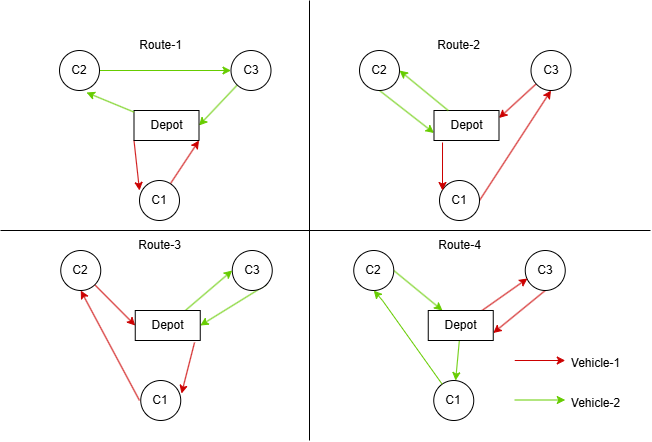
\includegraphics[scale=0.6]{Crest/Images/vrp_illustration.png}
    \caption{A sample of VRP routes with 2 vehicles and 3 customers.}
    \label{fig:vrp_illustration}
\end{figure}

Beyond this standard formulation, VRP has numerous variants \cite{vrp_survey}, including:
\begin{enumerate}
    \item Capacitated VRP (CVRP) in which each customer has a demand for a good and that vehicles have a limited capacity
    \item The VRP with pick-up and Delivery (PDP) in which the goods must be picked up and delivered in a certain amount at each vertex.
    \item  Heterogeneous Fleet VRP (HVRP), in which the vehicles have different capacities.
\end{enumerate}


\section{Ride-Sharing Problem}\label{Section22}
This PhD thesis presents models for a carbon-neutral dynamic ride-sharing service, so it is critical to grasp the concept of ride-sharing first, before exploring dynamic ride-sharing and its challenges. Traditionally, ride-sharing, also called carpooling, is the sharing of journeys so that more than one person travels in a car. It aims to bring travellers with similar itineraries and travel schedules together, which is mostly a commitment among travellers. Ride-sharing provides societal and environmental benefits such as sharing fuel costs, tolls, or other potential travel costs with other travellers, which can lower cost per traveller. It also leads to a reduction in GHG emissions and traffic congestion due to the reduced number of vehicles on the road.

\begin{figure}[htbp]
    \centering
    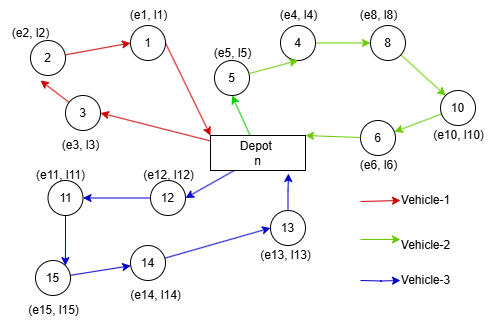
\includegraphics[scale=0.6]{Crest/Images/ride-share_illustration.png}
    \caption{Illustration of a VRP with 3 vehicles and 15 passengers.}
    \label{fig:vrptw}
\end{figure}

The ride-sharing problem combines the VRP with Time Windows (VRPTW) with the Dial-a-Ride Problem (DARP) \cite{paparella2024congestion} where the routing component of the VRP involves the movement of passengers between locations. This preliminary, basic version of the ride-sharing problem is a natural step from the broader VRP to the dynamic ride-sharing context. In this basic formulation, each customer must be visited (even if serving them late violates their designated time window), and all customers are ultimately brought back to the depot. Vehicles may arrive at a location before the designated time window begins; however, service cannot commence until the time window is officially open. In practice, arrivals after the stated time window are often disallowed (hard constraints), but a model may choose to accommodate such late arrivals by imposing penalty costs (soft constraints). In the fully strict or “hard” model, any route that serves a customer outside its time window is infeasible, and that customer would effectively remain unserved. In contrast, a “soft” model permits service outside the window but penalises lateness, ensuring every customer is still visited while acknowledging real-world flexibility in scheduling \cite{soa_rideshare}.

The formulation of the ride-sharing problem is dependent on the objectives and constraints under consideration \cite{asghari2021green}, and is generally defined by: 

\begin{itemize}
    \item A set of identical vehicles denoted by \( K \),
    \item A directed graph network \( G(N, A) \), where:
    \begin{itemize}
        \item \( N \): Set of nodes (customers and the depot),
        \item \( A = \{(i, j) : i \neq j, i, j \in N\} \): Set of vertices or directed routes between nodes.
    \end{itemize}
    \item Node \( 0 \) represents the central depot, while \( N^* = N \setminus \{0\} \) represent customers.
    \item The distance and transit time between two nodes is denoted as \( d_{ij} \) and \( t_{ij} \), respectively. The transit time depends on both static factors (as the distance) and dynamic factors (as the traffic at the given time the distance is traversed). In this PhD thesis, for simplicity of the proposed models, ride-sharing is restricted to static factors only; specifically, the transit time is assumed to be equal to the distance (\( t_{ij} = d_{ij} \)) (i.e., simulating a constant speed for traversing it). This assumption is made to decrease computational complexity and aid in the creation of traceable optimisation models. Incorporating dynamic elements like real-time traffic congestion would need integrating predictive models or real-time data streams, which would greatly increase processing overhead. Furthermore, such dynamic aspects bring unpredictability, making it difficult to obtain reproducible optimisation results. 
\end{itemize}

Each customer \( i \in N^* \) is characterised by:
\begin{itemize}
    \item \( q_i \): Travel Demand of the customer where the demand is pick up point and time and drop of point and time of customer \(i\),
    \item \( s_i \): Service time required at the customer,
    \item \( (e_i, l_i) \): Time window, where \( e_i \) is the opening time, and \( l_i \) is the closing time,
    \item \( a_i \): Arrival time of the vehicle at the customer,
    \item \( w_{ik} \): Waiting time of vehicle \( k \) at customer \( i \).
\end{itemize}

The decision variable \( x_{ijk} \) is defined as:
\[
x_{ijk} =
\begin{cases} 
1 & \text{if vehicle } k \text{ travels from node } i \text{ to node } j, \\
0 & \text{otherwise.}
\end{cases}
\]

Let \( y_i \) is a binary variable such that:
\[
y_i =
\begin{cases} 
1 & \text{if customer } i \text{ is served}, \\
0 & \text{otherwise.}
\end{cases}
\]

In this context, three potential goals for the ride-sharing problem are:

\begin{itemize}
    \item \textbf{Goal 1}: Minimise the total number of vehicles used.
    \item \textbf{Goal 2}: Minimise the total distance travelled.
    \item \textbf{Goal 3}: Minimise the number of customers not being served.
\end{itemize}

An objective function for the ride-sharing problem can be designed to focus on a specific goal or to simultaneously attempt to optimise multiple goals by applying a weight \( W_i \) to each separate goal:

\[
\min \left( W_1 \sum_{k \in K} \sum_{j \in N^*} x_{0j}^k + W_2 \sum_{k \in K} \sum_{(i, j) \in A} d_{ij} x_{ijk} + W_3 \sum_{i \in N^*} (1 - y_i) \right)
\]

In the formula above, \( W_1, W_2, \) and \( W_3 \) are weight factors that determine the priority assigned to each goal in the objective function. It is important to note that the third term maximises the number of TPs served by rewriting it in minimisation form, as minimising \( (1 - y_i) \) effectively maximises \( y_i \), which represents the number of customers served.

\textbf{The set of constraints to be satisfied by any valid solution of the ride-sharing problem is presented below:}
\begin{align}
    \sum_{i \in N} q_i \sum_{j \in N} x_{ij}^k &\leq q_{\text{max}}^k, \quad \forall k \in K \tag{3.1} \\
    \sum_{k \in K} \sum_{j \in N} x_{ij}^k =1, \forall i \in N \tag{3.2}\\
    \sum_{j \in N^*} x_{0j}^k =1, \forall k \in K \tag{3.3}\\
    \sum_{j \in N} x_{ij}^k - \sum_{j \in N} x_{lj}^k &= 0, \quad \forall l \in N, \forall k \in K \tag{3.4} \\
    \sum_{j \in N^*} x_{j0}^k &= 1, \quad \forall k \in K \tag{3.5} \\
    a_0 = w_{0}^k = s_0 &= 0 \tag{3.6} \\
   \sum_{j \in N} x_{ij}^k( a_i + w_{i}^k + s_i + t_{ij}) &\leq l_j, \quad \forall i \in N, \forall k \in K \tag{3.7} \\
    e_i \leq a_i + w_{ik} &\leq l_i, \quad \forall i \in N, \forall k \in K \tag{3.8} \\
    % x_{ij}^k &\in \{0, 1\}, \quad \forall (i, j) \in A, \forall k \in K \tag{3.9} \\
    y_i &\leq \sum_{k \in K} \sum_{j \in N} x_{ij}^k, \quad \forall i \in N^* \tag{3.9}
\end{align}

The constraint (3.1) states that the capacity of the vehicle (\(q_{\text{max}}^k)\) cannot be exceeded and constraint (3.2) that each customer must be served exactly once and by one vehicle. The set of constraints (3.3), (3.4) and (3.5) make sure that each vehicle starts from the depot {0}, visits and serves a certain number of customers, and finally returns to the depot {0}. Constraints (3.6), (3.7) and (3.8) indicate that for a trip from node i to node j, no vehicle may arrive at customer j after the end of the time window, (\(l_i)\). Constraints (3.9) ensures that a customer \( i \) is marked as served (\( y_i = 1 \)) only if there exists a vehicle \( k \) that travels to node \( i \). Simultaneously, the time of arrival to a customer, depends on the time of arrival, the waiting time and the service time, to the previous served customer. 

This MIP model provides a formulation of the general ride-sharing problem, serving as a foundation for more complex variations such as dynamic ride-sharing. An example of an instance for this ride-sharing problem, with 3 vehicles and 15 customers, is illustrated in Figure \ref{fig:vrptw}. The approach taken in Chapter  \ref{chapter3} differs as it incorporates real-time demand uncertainty and adaptability, which are not explicitly captured in this static MIP formulation. The following section delves into these challenges and the proposed solutions for dynamic ride-sharing. 


% \section{Ride-Sharing Services}
% \label{sec:ridesharing}

% Ride-sharing services extend the VRP by introducing paired pickup and drop-off locations for passengers, dynamic requests, and vehicle capacity constraints. This section highlights the unique aspects of ride-sharing compared to traditional VRP.

% \subsection{Concept of Ride-Sharing Services}
% Ride-sharing systems aim to transport multiple passengers efficiently by reducing the number of vehicles on the road, minimizing pollution, and lowering traffic congestion. These systems require vehicles to route dynamically between pickup and drop-off points, ensuring optimal passenger satisfaction while adhering to operational constraints.

% \subsection{Example: Ride-Sharing Problem}
% Consider an instance with 2 vehicles and 3 passengers, where each passenger has a distinct pickup and drop-off location:
% \begin{figure}[htbp]
%     \centering
%     \includegraphics[scale=0.6]{images/ridesharing_example.png}
%     \caption{Illustration of ride-sharing with 2 vehicles and 3 passengers.}
%     \label{fig:ridesharing_example}
% \end{figure}

% While there are multiple ways to route the vehicles, some trip petitions (TPs) may remain unsatisfied due to constraints like vehicle capacity or time windows. For example:
% \begin{itemize}
%     \item Vehicle 1 picks up Passenger A and drops them off but cannot pick up Passenger B due to time constraints.
%     \item Vehicle 2 can pick up Passengers B and C but cannot complete all trips without violating time windows.
% \end{itemize}
% This example highlights the importance of prioritizing TPs and optimizing routes to maximize trips served—a key objective of this PhD.


\section{Dynamic Ride-sharing Problem}
\label{sec:dynamic}
Nowadays, transportation, like many other aspects of daily life is being transformed by the information technology (IT) \cite{golob2001impacts}. The widespread use of mobile devices, as well as the development of the Global Positioning System (GPS), enable all transport operators to adapt transport supply to travel demand in real-time. These possibilities have resulted in the development and evolution of ride-sharing known as dynamic ride-sharing \cite{srinivasan2006impact, altshuler2017ridesharing}.

A dynamic ride-sharing service can be defined as a reactive VRPTW, in which TPs are released over time, while the vehicles may already be en route or stationed at different places \cite{kucharski2017realtime, liao2024towards}. This is distinct from a proactive or static VRPTW, in which all TPs are known in advance. 

To better grasp the dynamic feature of the service, Figure \ref{fig:dynamic_rs_illus} depicts the route execution of a single vehicle satisfying TPs. The vehicle plans an initial route to visit the currently known TPs (A, B, C, D, and E) before it departs the depot (time t0). At time t1, two additional petitions (X and Y) are released, leading to re-route of the vehicle in order to accommodate them. Finally, at time tf, the performed route is (A,B,C,D,Y,E,X).
\begin{figure}[htbp]
    \centering
    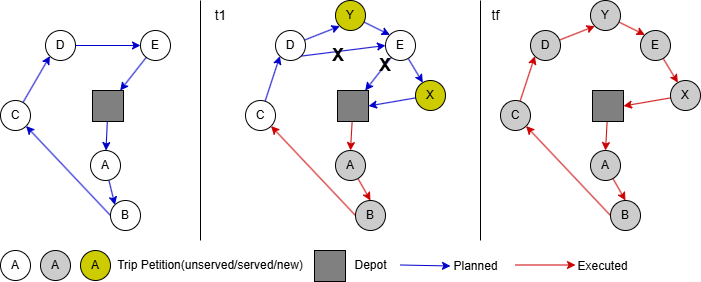
\includegraphics[scale=0.6]{Crest/Images/dynamic_ride_sharing_example.png}
    \caption{Example of dynamic ride-sharing}
    \label{fig:dynamic_rs_illus}
\end{figure}
This example demonstrates how dynamic TPs may lead to re-routing existing vehicles on an ongoing basis, necessitating real-time communication between vehicles and the dispatching centre. Figure \ref{fig:dynamic_routing} depicts a real-time communication example in which the \textit{dispatcher} is the agent that delivers instructions to the vehicle. When the vehicle is ready (first dotted arrow), the dispatcher makes a decision and directs it to complete petition A (first double headed arrow). When the vehicle begins (second dotted arrow) and stops (third dotted arrow) service at petition A, it alerts the dispatcher, who updates the available information and sends the vehicle its next request (second double-headed arrow).
\begin{figure}[htbp]
    \centering
    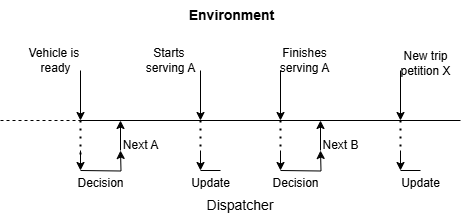
\includegraphics[scale=0.6]{Crest/Images/timeline_events.png}
    \caption{Timeline of events for the dynamic routing of a single vehicle}
    \label{fig:dynamic_routing}
\end{figure}

This PhD thesis considers the following key features in order to accommodate dynamic ride-sharing:

\textbf{Time Dimension:} 
The dispatcher must have precise knowledge of the location of all vehicles at any time, in order to respond effectively to service new upcoming TPs or other dynamic information.

% \textbf{Near-Term Events are More Important:} 
% Dynamic routing requires prioritisation of near-term events, as it would be risky to allocate vehicle resources prematurely to long-term requirements. Dispatchers in dynamic scenarios must focus on addressing immediate demands.

\textbf{Information Update Mechanisms are Essential:} 
In dynamic routing environments, system inputs such as new TPs or vehicle availability evolve continuously over time. To maintain solution feasibility, the routing process must incorporate update mechanisms—these refer to procedures or algorithms that periodically or event-drivenly revise vehicle routes, schedules, and resource allocations based on the most recent system state. For example, when a new TP is submitted or an AEV becomes available after completing a task, the routing solution is recalculated to integrate this information. Such mechanisms are unnecessary in static settings, where all system inputs are fixed and known in advance.

\textbf{Re-sequencing and Re-assigning Decisions May Be Warranted:} 
New inputs in dynamic routing can turn previously made decisions as sub-optimal in light of the new context. As a result, dispatchers may need to re-route or re-assign vehicles to adapt to new circumstances and maintain efficiency.

\textbf{Faster Computation Times Are Necessary:} 
In static routing, dispatchers might afford longer computation times to obtain high-quality or even optimal solutions. However, in dynamic scenarios, dispatchers most likely need to generate solutions quickly (perhaps within minutes or seconds) in order to address the immediate problem. This time constraint often necessitates the use of local improvement heuristics, such as insertion and \(k\)-interchange, for re-routing and re-assignments.
Local improvement heuristics are a class of optimisation techniques designed to refine existing solutions by making small adjustments iteratively \cite{cordeau2007dial, gendreau1994tabu}.  
\begin{itemize}
    \item \textbf{Insertion Heuristic}: This method involves inserting a new request (or modifying an existing one) into an existing route in a way that minimises additional cost. It evaluates various potential insertion points and selects the one that results in the least disruption to the current schedule \cite{jaw1986heuristic}.
    \item \textbf{\(k\)-Interchange Heuristic}: This heuristic swaps up to \(k\) requests between different routes to improve overall efficiency. By exchanging a subset of trips between different vehicles, the method aims to balance loads, reduce travel time, or optimise service times \cite{potvin1993kinterchange, berbeglia2010dynamic27}.
\end{itemize}
These heuristics enable dispatchers to generate feasible solutions in real-time, making them particularly useful in dynamic routing scenarios where computational speed is critical.

\textbf{Objective Functions in Dynamic Settings May Differ from Those in Static Routing Problems:} 
In conventional static vehicle routing or ride-sharing models, objective functions often focus on minimising total travel distance, total service time, or the number of vehicles used, with all trip demands known in advance. However, in dynamic ride-sharing environments where TPs are continuously generated, vehicles are reallocated in real-time, and system states evolve unpredictably, such static objectives may lose relevance. Optimisation strategies in such contexts must operate on partial information, incorporating real-time data and, where possible, probabilistic estimations of future events to ensure effective service performance \cite{spall2003introduction}.

\textbf{Time Constraints May Be More Flexible:} 
In dynamic routing problems, time constraints such as latest pickup times are often more flexible than in static problems. Denying service to an imminent demand due to a minor breach of time constraints is generally less desirable than accommodating the request by relaxing these constraints \cite{ichoua2003vehicle}.

\textbf{Centralised vs Decentralised Approaches:} In a centralised system, a central unit collects and processes all \cite{alonso2017demand}, adding to the complexity of the dynamic ride-sharing problem. In a decentralised system, the vehicle itself or an aggregator could process some of the information. This depends on the ride-sharing fleet provider and is explored further in the following section.

% \begin{enumerate}
%     \item \textbf{Time Dimension is essential:} In a static routing problem, the time dimension may or may not matter. In a dynamic counterpart, time is always important. In response to service requests or other information, the dispatcher must know the location of all cars.

%     \item\textbf{Near-term events are more important:} BeIn a static routing problem, all events receive equal weight due to the homogeneity of information quality and the absence of input updates. In a dynamic situation, it would be imprudent to quickly devote vehicle resources to long-term requirements. When dealing with a dynamic routing problem, the dispatcher should prioritise near-term events.

%     \item\textbf{Information update mechanisms are essential:} Almost all inputs to a dynamic routing problem can alter during the day of operation. It is consequently necessary to incorporate information update techniques into the solution procedure. Naturally, information update techniques are irrelevant in a static setting.

%     \item\textbf{Re-sequencing and reassigning decisions may be warranted:} In dynamic routing, fresh input may cause the dispatcher's decisions to become suboptimal. This causes the dispatcher to reroute or even reassign vehicles in order to address the new scenario.

%     \item\textbf{Faster computation times are necessary:} In static settings the dispatcher may a ord the luxury of waiting for a few hours in order to get a high quality solution, in some cases even an optimal one. In dynamic settings this is not possible, because the dispatcher wishes to know the solution to the current problem as soon as possible (preferably within minutes or seconds). The running-time constraint implies that rerouting and reassignments are often done by using local improvement heuristics like insertion and k-interchange.

%     \item \textbf{Indefinite deferment mechanisms are essential:} Indefinite deferment refers to the possibility that the service of a certain demand may be postponed indefinitely due to the demand's unfavourable geographical qualities in comparison to the other demands. This problem could be solved by employing time window constraints or a nonlinear objective function that penalises excessive waiting.

%     \item \textbf{Objective function may be different:} Traditional static objectives, such as minimising total distance travelled or overall schedule duration, may be meaningless in a dynamic situation where the process is open-ended. If no knowledge about future inputs is available, it may be appropriate to optimise just over known inputs. Some services employ nonlinear objective functions to avoid unwanted events such as the aforementioned infinite deferment.

%     \item\textbf{Time constraints may be different: } Time limitations, such as the latest pickup times, are softer in dynamic routing problems than in static ones. This is owing to the fact that denying service to an imminent demand if the time constraint is not satisfied is typically less appealing than breaching it.
% \end{enumerate}

% In summary, dynamism can be defined as:
% \begin{itemize}
%     \item A problem is dynamic if its parameters change over time. This includes models with dynamic data that change constantly as well as problems with time-dependent data that are known in advance.

%     \item A model is dynamic if it explicitly incorporates the interaction of activities over time. Here one should distinguish between deterministic dynamic models and stochastic models.

%     \item If an application solves the underlying model repeatedly as new information comes in, it is considered dynamic.Subsequently, solving models within dynamic applications requires huge computational resources.
% \end{itemize}

The primary components of the dynamic ride-sharing service are the passenger, vehicle, and matching algorithm. The passenger seeks a ride that will pick her/him up at the starting place and drop her/him off at the desired destination within a time frame. The transportation provider has a fleet of vehicles (taxi, van, autonomous vehicle, etc.) ready to satisfy the needs of a passenger. The matching and routing algorithm gets requests and fleet information and attempts to find the best matches on short notice. As co-operation/collaboration between different fleet providers is critical for this PhD thesis and the models it proposes, the different key aspects defining such potential co-operation/collaboration are described in Figure \ref{fig:rideshare_category}. Fleet providers can operate either competitively or cooperatively. In a competitive planning approach, fleet providers are competitors, and they hesitate to share information about their cost structures and TPs  \cite{agatz2012optimization}. Relying on a neutral dispatcher to re-assign jobs within the system establishes the compensation and profit sharing framework. These scenarios are referred to as centralised competitive planning approaches. On it, a neutral, centralised dispatcher attempts to address the whole set of TPs, notifying each fleet provider of the ones assigned to it \cite{agatz2012optimization}.

\section{Decentralised Dynamic Ride-sharing }
\label{sec:decentralised}

In the case of cooperative interaction, providers exchange fleet information, making it easier for the passenger to get a ride and increasing the benefits of ride-sharing \cite{shen2018integrating}. For a decentralised approach, the fleet providers have to reveal only a small proportion of the information they would have to disclose in a centralised approach \cite{klapp2020decentralized}. For instance, in a centralised system, fleet providers must share their complete availability, pricing structures, and operational constraints with a central authority, which can lead to concerns over data privacy, competition, and strategic disadvantages. In contrast, a decentralised approach allows fleet providers to retain autonomy by only disclosing essential details such as available capacity or general service regions, reducing information overhead while maintaining independence. This PhD thesis focuses in both centralised and decentralised approaches for cooperative ride-sharing. In both cases, the effectiveness of the system relies on the matching and routing algorithm allowing to maximise the trips served.

A dispatcher receives the TP info from each passenger. It also gets access to the fleet being able to monitor the position, route and passenger allocation of each vehicle at any given time. The system processes the passenger TPs as they arise, potentially re-routing an existing vehicles to pick up and drop off the new passenger as requested \cite{masoud2017decentralized}. Despite the limited practical use of centralised collaborative approaches, due to trust issues, solving the centralised problem remains critical for this PhD thesis, even if only as a benchmark for its comparison with counterpart decentralised approaches. 

Figure \ref{fig:collaborative} illustrates a scenario with and without collaboration (respectively top and bottom of the figure) for a routing problem involving three carriers. The figure is based on equal workloads, meaning each vehicle tries to serve an equal number of TPs. 

\begin{figure}[htbp]
    \centering
    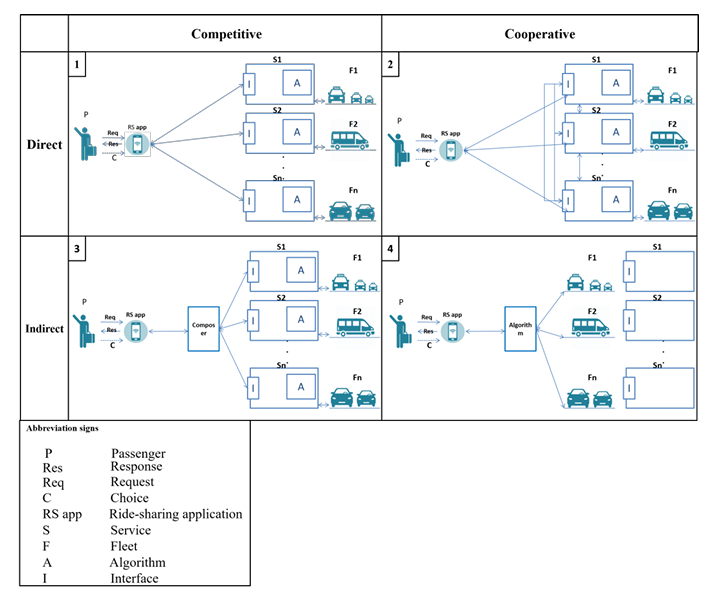
\includegraphics[scale=0.6]{Crest/Images/dynamic_rideshare_category.png}
    \caption{Different categories of dynamic ride-sharing \cite{soa_rideshare}}
    \label{fig:rideshare_category}
\end{figure}

In the collaborative scenario (bottom part of the figure), carriers are able to exchange TPs, leading to a more efficient overall allocation of resources. This results in shorter total travel distances, reduced vehicle idle time, and more balanced route distributions across the carriers. The exchange of requests allows each vehicle to focus on a more geographically compact set of requests, which reduces unnecessary detours and increases overall service efficiency. 

In contrast, in the non-collaborative scenario (top part of the figure), each carrier is limited to serving only its originally assigned requests, which leads to longer and less efficient routes. Some carriers may end up with routes that have excessive travel distances, while others might experience underutilisation. 

It is evident that every carrier would significantly benefit from these exchanges as they reduce operational costs, improve service times, and create a more balanced workload distribution among the fleets. The models show in chapters \ref{chapter4} and \ref{chapter5} of this PhD will be based on such these collaborative setting.

\begin{figure}[htbp]
    \centering
    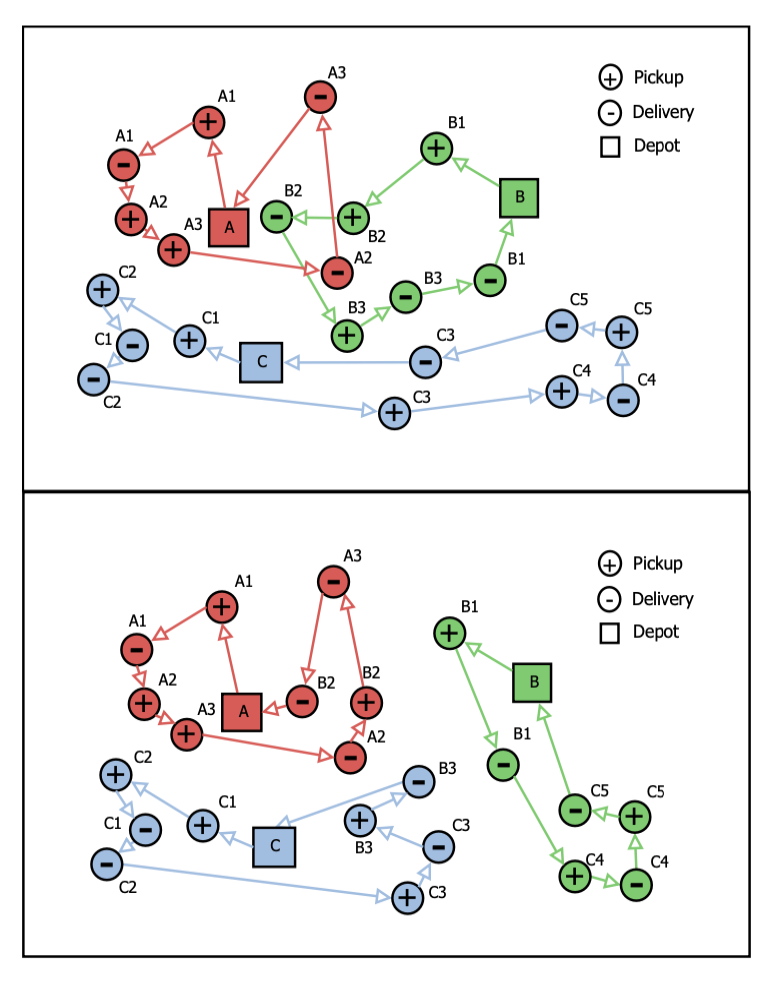
\includegraphics[scale=0.6]{Crest/Images/collaborative_routing.png}
    \caption{Example of non-collaborative planning(top) and collaborative(bottom) planning}
    \label{fig:collaborative}
\end{figure}

\section{Autonomous Electric Vehicles (AEV)}
\label{sec:aevs}
Another significant innovation that has the potential of impact ride-sharing services in the coming decades is the introduction of Autonomous Electric Vehicles (AEVs). 
The following definition by the author \cite{fagnant2014future} represents the term “Autonomous Vehicle” (AV) as used in this PhD thesis:
\textit{Autonomous vehicles are vehicles that can drive without human intervention or monitoring in an unpredictable, uncertain, and open traffic environment designed, built, and populated by and for humans. It represents the highest level of autonomy and thus the ideal future end-state of these vehicles.} 

One of the challenges associated with ride-sharing is the limitations faced by a vehicle due to the availability of its owner to drive it. Incorporating AEVs into the system would prove instrumental in removing these limitations (allowing each vehicle for 24/7 service) while also reducing emissions, enhancing street safety, saving time and space, and reducing congestion. The PhD thesis focuses on using AEVs for ride-sharing for the above-mentioned reasons.

\section{Smart Energy Communities (SECs)}
\label{sec:secs}

The ride-sharing models proposed in this PhD thesis are based on the use of SECs. These can be defined as: (1) AEV depots, (2) cooperative dispatchers, and (3) localised energy hubs. The SECs represent the solely source for charging the AEV fleet of the ride-sharing service. Specifically, they make the service carbon-neutral, by using solely the RES generated by each SEC (e.g., solar and wind power) to charge the vehicles \cite{paranjape2020urban}. By restricting itself to operate under 100\% RES, the SECs-based ride-sharing service often face resource constraints. For example, on a given day, one of the SECs of the ride-sharing service owning a total of 10 AEVs, may only generate enough energy to charge 5 of them during peak ride-sharing service hours (therefore not being able to use the other 5 EVs at all, which remain idle at the SEC depot). It is in the context of this resource scarcity that the ride-sharing service will benefit from the intelligent scheduling and resource allocation models proposed in this PhD thesis.

A key feature of SECs is their ability to engage in cooperative strategies with neighbouring SECs, enabling shared resource utilisation \cite{peterson2020integrating}. However, to ensure effective cooperation, the challenges such collaboration introduce must be addressed, including:
\begin{itemize}
    \item \textbf{Efficient Fleet Allocation:} Determining which EVs to dispatch and where, without disrupting local operations.
    \item \textbf{Equitable Reward Mechanisms:} Designing incentives that fairly compensate SECs for contributing resources while fostering long-term collaboration.
    \item \textbf{Real-Time Decision Making:} Adapting to dynamic demand and energy availability in real-time while minimising computational delays.
    \item \textbf{Sustainability Trade-offs:} Balancing operational efficiency with carbon-neutral objectives, especially when collaboration may increase travel distances for EVs.
\end{itemize}

As an example of the benefits of such collaborations, suppose SEC A has a fleet of AEVs primarily serving TPs within its region, but it receives an unusually high demand for rides due to a local event. Meanwhile, SEC B, located nearby, has surplus fleet capacity because its demand is relatively low at the same time. The two SECs can then negotiate a fleet allocation arrangement:
\begin{itemize}
    \item \textbf{Negotiation Terms:} SEC A can request a SEC B to dispatch a number of its AEVs to serve some of the TPs SEC A is facing. In return, SEC A offers to compensate SEC B with either charging credits at its AEV charging facilities and/or with the promise of future fleet assistance on a potential future time peak demand period for SEC B.
    \item \textbf{Outcome:} A number of AEVs from SEC B temporarily operate serving some of the TPs SEC A is facing reducing unmet trip demand in SEC A while ensuring such AEVs from SEC B remain operationally utilised rather than idle. This negotiation dynamically balances resource utilisation across SECs, improving the overall service efficiency of the ride-sharing service.
\end{itemize}

This example underscores how negotiation and incentive systems between SECs can address demand fluctuations and resource constraints. The ride-sharing network enhances its overall efficiency by carrying out inter-SEC negotiations leading to dynamically re-allocation of AEVs. These mechanisms contribute to the efficiency of the ride-sharing service, specially in light of the aforementioned carbon neutrality restrictions. Further discussions on the design and implementation of these collaborative strategies are provided in chapters \ref{chapter4} and \ref{chapter5}. To the best of our knowledge, this is the first study that leverages SEC in this context to build a carbon-neutral dynamic ride-sharing service. 

\section{Charging Infrastructure}
\label{sec:charging}

Integrating AEVs into ride-sharing introduces several challenges, such as restricted battery capacity and downtime during charging operations. These issues are especially significant in the context of the aforementioned carbon-neutral, AEV and SECs-based ride-sharing service described in this PhD thesis, where efficient charging solutions are critical to minimising downtime, ensuring AEV availability, and ultimately maximising the number of trips served. 

To address these challenges, this PhD thesis incorporates strategies for managing AEV charging infrastructure where AEVs are charged at its home SEC, using its locally generated RES available at the time of charging.
Alternatively, an AEV can also charge at a neighbouring SEC, through resource sharing agreements between the host and home SECs as the ones aforementioned described.

Determining the optimal placement for a network of charging stations is a complex problem which is outside the scope of the PhD thesis. In its simplest form, the problem can be modelled as a \textit{facility location problem} \cite{ortiz2018multi}, where the goal is to identify the best locations for AEV depots that also function as charging stations. Alternatively, when a charging station location is interdependent with the routing of the AEVs it hosts, the problem becomes a \textit{location routing problem} \cite{ortiz2018multi}. Planning charging stops within a dynamic ride-sharing service introduces additional complexity due to several interrelated factors. Firstly, the dynamism of ride requests leads to rapidly changing demand patterns, requiring real-time adjustments in vehicle routing and charging schedules. Secondly, time window constraints limit the time during which AEVs can service trips or reach charging stations, necessitating precise coordination to avoid delays or missed requests. Lastly, the need to balance energy availability and trip demands within the network further complicates scheduling, as vehicles must strategically allocate charging opportunities without compromising service efficiency.

The optimisation challenge faced in this PhD thesis is to, given (1) a static network of charging stations (each of them belonging to one of the SECs of the ride-sharing service), (2) a number of AEVs owned by the SECs and (3) a number of TPs, each of them with a weight indicating its importance, decide the schedule of the charging of the AEVs fleet, in such a way it maximises the overall weight of the TPs being served.

To illustrate the challenge, consider the following scenario, where SEC A:

\textbf{Scenario}, SEC A operates a fleet of 10 AEVs, supported by solar panels generating 50 kWh of renewable energy daily. Each AEV requires 60 kWh for a full charge, enabling 100 km of travel. Due to high demand, SEC A needs to prioritise which AEVs are to be charged in order to maximise trip fulfillment. This challenge differs when tackled in the context of AEVs solely charged by their home SECs vs. the context of different SECs negotiating and, therefore, cooperating in the AEVs charging. Each scenario is discussed separately below:

\textbf{Charging Process at Home SEC:} SEC A schedules its charging operations by prioritising those AEVs with a planning route containing the most significant TPs, but resulting in risk of running out of battery if more TPs are added to their route. For instance, EV 1, with 20\% battery, is scheduled for immediate charging to ensure availability for an upcoming ride request. On the other hand, EV 2, with 60\% battery, is placed in a lower priority queue since it is much more likely to be able to accommodate at least one more trip before requiring a battery charge.

\textbf{Charging at Neighboring SECs}: During peak demand, SEC A negotiates with SEC B to charge some of its AEVs. For instance, if an AEV is low on battery and located closer to SEC B than SEC A, it charges at SEC B instead. In return, SEC A compensates SEC B with energy credits or other incentives, ensuring efficient energy distribution and reducing strain on individual SECs.

As a result, such collaborative charging mechanisms help to:
\begin{itemize}
    \item Maximise AEV utilisation by reducing the time spent travelling to a charging station. In the example above, SEC A can serve additional TPs by focusing its local resources on more urgent charging needs.
    \item Enhance the flexibility of the ride-sharing network, allowing SECs to handle peak demands efficiently.
    \item Contribute to the carbon neutrality of the ride-sharing service by optimising the use of RES across SECs.
\end{itemize}

This PhD thesis designs, implements and evaluates models to address the optimisation challenges outlined above, ensuring efficient scheduling of charging operations while maintaining SEC collaboration. Chapter \ref{chapter5} details these solutions, including real-time scheduling strategies and dynamic incentive mechanisms to foster inter-SEC cooperation.

\section{Literature Review}
\label{sec:literature_review}
This section examines the existing literature on dynamic ride-sharing, vehicle fleet allocation, and charge scheduling. The primary goal is to review existing work, so as to better position the specific contributions and challenges addressed by the ride-sharing models proposed in this PhD Thesis.

\section{Dynamic Ride-sharing}
Dynamic ride-sharing involves real-time matching of TPs with available vehicles while optimising fleet utilisation. Unlike static ride-sharing, where routes are planned in advance, dynamic ride-sharing solutions must continuously adapt to new requests, cancellations, and fluctuating demand. Widely studied in operations research and transportation literature [101], the complexity of the problem arises from its multiple constraints and objective functions, which has lead to a number of solution methods to tackle it \cite{meng2021dynamic}.

\subsection{Constraints and Objective Functions}
\label{objectives_constraints}
The constraints and objective function determines the variant of the dynamic ride-sharing problem being considered. Table \ref{table:problem_inputs} surveys the existing literature to classify the constraints and objective functions being considered.

\begin{table}[htbp]
\centering
\renewcommand{\arraystretch}{1.2} 
\setlength{\tabcolsep}{4pt} 
\small 
\begin{adjustbox}{max width=\textwidth}
\begin{tabular}{|p{3.5cm}|p{11cm}|}
\hline
\textbf{Category}            & \textbf{Key Attributes} \\ \hline

\multirow{1}{3.5cm}{\textbf{Transportation Demand}} 
& Time-dependent demand, real-time trip hailing, authentication system, trip motivation, origin, destination, seat demand, maximum waiting time, maximum travel time, maximum detour, maximum fare, time window, desired pick-up and drop-off times, delay tolerance, sharing limit, distance from origin to pick-up, departure time, arrival time. \\ \hline

\multirow{1}{3.5cm}{\textbf{Transportation Service}}
& Vendors, fixed fleet, timetables, fixed stops, waiting locations, homogeneous/heterogeneous vehicle fleet, professional vs. non-professional supply, vehicle capacity, pricing schemes. \\ \hline

\multirow{1}{3.5cm}{\textbf{Algorithmic Considerations}} 
& Objective function, dispatching, searching, scheduling, monitoring, shortest path computation, empty vehicle behaviour, accept/reject TPs, traffic considerations. \\ \hline

\end{tabular}
\end{adjustbox}
\caption{Problem attributes considered in dynamic ride-sharing}
\label{table:problem_inputs}
\end{table}

\textbf{Objective Functions}: In terms of the desired goal, most approaches aim to find the near-optimal solution to the matching problem in ride-sharing services by considering specific objective functions, such as minimising the total travel distance or time \cite{ota2017stars135, qian2017optimal143, dorey2014ridesharing53} and maximising the match between vehicles and passengers \cite{stiglic2016making162, ma2013tshare118, goel2017optimal68, herbawi2012ridematching80, berbeglia2012hybrid28, stiglic2015benefits161, santos2015taxi152} and minimising the number of required vehicles \cite{kirchler2013granular96, lehuede2014multicriteria107}, or vehicle emissions \cite{atahran2014multicriteria22}. 

Travel duration and distance are crucial factors for travellers \cite{naoum2015stochastic133}. Real-time approaches, like \cite{delling2009engineering}, efficiently compute the shortest path in real time. Non-real-time techniques, such as the proposed method in T-Share \cite{ma2013tshare}, can estimate the distance of the shortest path by partitioning the street network into grid cells and determining the shortest path for each anchor node (the nearest node in the road network to the geographical centre). 

Another significant goal for passengers is to minimise the amount of time they have to wait for their journey. Typically the primary aim of passengers is to save money on their trip. According to \cite{stiglic2016making162}, if no match is identified within a certain time frame, passengers are more likely to abandon the system and refuse to use shared mobility services. Minimising total passenger trip or waiting time may improve performance for passengers, but not for the system as a whole. Reducing passenger wait time can make shared services comparable to typical taxi services. Various techniques in the literature strive to decrease the waiting for passengers as an objective function, such as \cite{hyland2018sharing87, kirchler2013granular96, masoud2017using126}. Much of the research on dynamic ride-sharing services focusses on a single provider. These studies typically incorporate restrictions for the problem to retain the passengers aim at an appropriate level \cite{molenbruch2017typology128, calvo2004distributed38}. Theses studies do not take into account multiple objectives unlike the one presented in this PhD thesis, where maximising trips served by using only the available RES is set as a hard constraint.  

In \cite{dorey2014ridesharing53}, total travel distance, taxi stand departures (number of exits from all taxi stands), and revenue per travel distance (revenue per km earned by all vehicles) were used to measure the performance of a vehicle owner in terms of operation mode and costs for all trips. The percentage of served requests, waiting time, journey time, and trip fee are used to determine the preferences of the passengers'. In \cite{kirchler2013granular96}, the authors included six objectives: Routing costs, excess ride time, passenger waiting time, route durations, early arrival times at pickup and delivery nodes, and the number of unfulfilled requests are all minimised.

% \subsubsection{Problem Constraints Categories}
% \label{problem_constraints}
\textbf{Constraints: }In the ride-sharing problem, a set of constraints and features must be taken into account for both transportation demand and transportation service. The constraints of the dynamic ride-sharing problem can be classified into four main categories:

\textbf{Assignment Constraints} ensure that each passenger is assigned to exactly one vehicle and that each trip follows the correct sequence from pick-up to drop-off \cite{stiglic2018enhancing163, goel2017optimal68}. Assignment constraints are the first restrictions of a ride-sharing problem and as a result, assignment limitations are hard constraints that must be satisfied when solving a ride-sharing problem. This has been modelled using a variety of ways in literature. In \cite{stiglic2018enhancing163}, the authors define an intermediary site called a meeting point for passenger pickup or drop off. They show that this meeting place can result in shorter detours. In \cite{goel2017optimal68}, the authors propose a ride-sharing approach where pick-up/drop-off locations are chosen from a fixed set. They describe a strategy for selecting ideally fixed Pick Up Points (PuPs) with the goal of maximising car occupancy rates while maintaining user privacy and safety. In \cite{naoum2015stochastic133}, the drop-off place is a common destination such as a university or company. Other studies focus on supplying passengers door-to-door in order to provide better comfort for sharing participants. In \cite{ota2017stars135, li2016share110, tachet2017scaling165}, passengers can specify pick-up and drop-off locations. In \cite{dorey2014ridesharing53, farin2016framework56, kleiner2011mechanism98}, the pick-up point is the current position of the passenger, and the only location specified is a trip destination.

\textbf{Synchronisation Constraints} maintain consistency in passenger transfers and ensure that multi-leg trips align with scheduling requirements \cite{fink2019column58, drexl2012synchronization54}. Synchronisation constraints are particularly relevant in dynamic ride-sharing systems where passengers may need to transfer between vehicles or where fleets are managed across different providers. In such scenarios, ensuring the coordination of pick-up and drop-off times between dependent trips is essential to avoid excessive waiting times and service disruptions \cite{masoud2017using126, lazzaretti2021real}. 
Beyond passenger transfers, synchronisation constraints also apply to energy constraints in electric vehicle-based ride-sharing services. Vehicles may need to synchronise their trips with available charging opportunities to ensure uninterrupted service, a challenge explored in depth in Chapter \ref{chapter5}.

\textbf{Time Window Constraints} require that passengers are picked up and dropped off within acceptable time limits. In some models, soft constraints allow minor violations with penalty costs \cite{agatz2011dynamic7, naoum2015stochastic133}, but must of the literature on ride-sharing considers the time windows as hard constraints. TSuch time windows are defined using various ways: In \cite{agatz2011dynamic7}, the passenger sets the earliest departure time and time flexibility, which is the difference between the earliest departure time and the latest arrival time. In \cite{naoum2015stochastic133, wang2018stable173, herbawi2012ridematching80, agatz2011dynamic7}, passengers specify the earliest and latest pick-up and arrival times. As a result, the passenger shall be picked up at the origin point no sooner than the specified pick-up time and left off at the destination before the latest arrival time. In \cite{linares2016simulation87}, travellers face implicit rather than explicit time limitations, and the objective function solely takes into account passenger waiting times.

\textbf{Capacity Constraints} restrict the number of passengers assigned to a vehicle based on its seating capacity. Some research aim to utilise the full capacity of the vehicle \cite{goel2017optimal68, dorey2014ridesharing53}. In addition to limiting the maximum number of passengers, studies on van-pooling systems set a minimum number of passengers to create a van-pool for a shared trip \cite{kaan2013vanpool93}. 

In this PhD thesis, capacity constraints are particularly relevant due to the integration of AEVs within SECs. Unlike conventional ride-sharing services that can dispatch additional vehicles when demand spikes, SEC-based ride-sharing services operate under RES constraints, which limit the number of AEVs available at any given time. As a result, it is critical to maximise vehicle occupancy while ensuring that capacity of each AEV is fully utilised to minimise the number of unserved TPs \cite{stiglic2018enhancing163, liu2020optimizing}.

Moreover, in SEC-based ride-sharing, capacity constraints must also consider energy availability. If the battery level of an AEV is low and charging resources are limited, the number of passengers that can be served on a single trip must be carefully managed to ensure that the vehicle can complete its route without requiring an unscheduled recharge \cite{hu2020electric}. This introduces a dual-layered capacity constraint, where both passenger occupancy and battery capacity influence the availability of the vehicles for ride-sharing.

Additionally, ride-sharing services operating with fleet collaboration mechanisms must incorporate fleet-wide capacity management. If an SEC cannot fulfil a ride request due to local vehicle shortages, it may dynamically allocate ride requests to neighbouring SECs. However, this requires strict coordination of available vehicle capacities across multiple SECs while maintaining service efficiency \cite{yang2021dynamic}.

This PhD thesis addresses these capacity constraints by developing an optimisation model that dynamically assigns vehicles based on real-time demand and energy availability. The model prioritises high-occupancy ride matches while ensuring that AEVs remain operational under energy constraints. The methodology and detailed formulation of this model are presented in Chapter \ref{chapter5}.

Table 2.2 provides a structured overview of the primary constraints considered in the literature for dynamic ride-sharing services. It is important to highlight that all these constraints are incorporated within the optimisation models proposed in this PhD Thesis.

While some prior studies incorporate energy constraints, they primarily address vehicle battery capacity or charging limitations in isolation, often assuming access to a static or grid-based energy supply. Unlike such approaches, this PhD thesis explicitly models the impact of renewable energy availability within SECs on ride-sharing feasibility. The energy constraints in this work are directly linked to the fluctuating, decentralised generation profiles of SECs, affecting vehicle dispatch, scheduling, and fleet coordination in real-time. This integrated approach ensures that both transportation and energy resources are jointly optimised, with the objective of maximising the number of trip petitions served under renewable energy constraints.


\begin{table}[ht]
\centering
\label{tab:constraints_table}
\renewcommand{\arraystretch}{1.5}
\resizebox{\textwidth}{!}{%
    \begin{tabular}{|l|c|c|c|}
        \hline
        \textbf{Constraint Type} & \textbf{Relevant Studies} & \textbf{Energy Constraint} & \textbf{Included in This PhD}  \\ \hline
        Assignment   & \cite{stiglic2018enhancing163, goel2017optimal68, naoum2015stochastic133, ota2017stars135, li2016share110, tachet2017scaling165, dorey2014ridesharing53, farin2016framework56, kleiner2011mechanism98} & No & Yes  \\ \hline
        Synchronisation & \cite{fink2019column58, drexl2012synchronization54, tachet2017scaling165, farin2016framework56, goel2017optimal68, masoud2017using126, lazzaretti2021real} & No  & Yes  \\ \hline
        Time Window   &  \cite{agatz2011dynamic7, naoum2015stochastic133, wang2018stable173, linares2016simulation87, herbawi2012ridematching80, agatz2011dynamic7} & No  & Yes \\ \hline
        Capacity  & \cite{goel2017optimal68, dorey2014ridesharing53, tachet2017scaling165, stiglic2018enhancing163, liu2020optimizing, hu2020electric, yang2021dynamic} & Battery Capacity / Charging Limits only  & Renewable Energy-Aware Fleet Coordination \\ \hline
    \end{tabular}%
}
\caption{Summary of problem constraints in dynamic ride-sharing. While some studies address energy constraints such as battery capacity or charging requirements, this PhD uniquely incorporates renewable energy availability from decentralised sources (SECs) into vehicle coordination and ride-sharing feasibility.}
\end{table}



\subsection{Solution Methods}
\label{solution_methods}
Solving the dynamic ride-sharing problem requires a balance between computational efficiency and solution quality. The complexity of the problem stems from its NP-hard nature, meaning that exact solutions become computationally intractable for large-scale instances.To address this, three primary solution approaches are explored in the literature: Exact methods, Heuristics, and Metaheuristics.
\begin{itemize}
    \item Exact Methods: These methods, provide optimal solutions but are computationally expensive. They are mainly used for small problem instances \cite{cordeau2007dial46, ropke2009branch148}. Exact approaches include:
    \begin{enumerate}
        \item \textbf{Mixed Integer Programming (MIP):} Formulates ride-sharing as an integer optimisation problem, typically solved using commercial solvers like CPLEX or Gurobi \cite{cordeau2007dial46, ropke2009branch148}.
        \item \textbf{Branch-and-Bound}: Systematically explores the solution space by pruning suboptimal solutions \cite{cordeau2007dial46}.
        \item \textbf{Branch-and-Cut}: An extension of Branch-and-Bound that includes cutting plane techniques to improve computational efficiency \cite{ropke2009branch148}.
        \item \textbf{Column Generation}: Used in large-scale formulations to iteratively generate variables that improve solution quality \cite{ghilas2018branch65}.
    \end{enumerate}
    
    \item Heuristic Methods: These methods offer computationally efficient alternatives by finding near-optimal solutions within reasonable time frames. These methods are particularly effective for large-scale ride-sharing instances.In general, heuristic approaches rely on one or more of the following criteria to dynamically make decisions without further reconsidering them:
    \begin{itemize}
        \item \textbf{Greedy Selection:} Prioritising assignments based on minimising cost functions such as shortest travel distance, minimum detour, or maximum service rate \cite{lu2021optimal}.
        \item \textbf{Insertion Heuristics:} Constructing solutions incrementally by inserting requests into existing routes based on predefined feasibility rules \cite{hyland2018sharing87}.
        \item \textbf{Ride-Matching Heuristics:} Ranking potential matches for passengers and vehicles based on similarity of origin-destination pairs, departure time, and detour tolerance \cite{stiglic2016making162, ma2013tshare118}.
        \item \textbf{Load Balancing:} Distributing requests across vehicles to avoid overloading specific regions of the network while ensuring equitable fleet utilisation \cite{goel2017optimal68}.
        \item \textbf{Time Window Constraints:} Making assignments that ensure pick-ups and drop-offs occur within predefined acceptable limits \cite{qian2017optimal143, dorey2014ridesharing53}.
        \item \textbf{Penalty-Based Adjustments:} Allowing minor violations of constraints (such as time windows or detour limits) with penalty costs incorporated into the objective function \cite{hyland2018sharing87}.
    \end{itemize}
    
    \item Metaheuristic Methods: These methods extend heuristics by incorporating\textbf{ stochastic or evolutionary techniques} to explore the solution space. Examples of these techniques include:
    \begin{enumerate}
        \item \textbf{Genetic Algorithms (GA)}: Uses evolutionary selection, mutation, and crossover operators to iteratively refine solutions \cite{herbawi2012genetic81}.
        \item \textbf{Local Search (LS)}: Progresses from an initial feasible solution by iteratively moving to a neighbour with a better objective value \cite{Crama1995}.  
        \item \textbf{Simulated Annealing (SA)}: Gradually reduces search randomness to settle on high-quality solutions \cite{ameli2019heuristic16}.
        \item \textbf{Large Neighbourhood Search (LNS)}: Iteratively removes and reinserts parts of the solution to escape local optima \cite{braekers2016multi35}.
        % \item \textbf{Tabu Search}: Employs memory structures to prevent cycling back to recently explored solutions, helping avoid premature convergence \cite{jung2016dynamic92}.
    \end{enumerate}
\end{itemize}

% \begin{table}[ht]
% \centering
% \caption{Comparison of Dynamic Ride-sharing Solution Approaches}
% \label{tab:solution_methods}
% \renewcommand{\arraystretch}{1.5}
% \resizebox{\textwidth}{!}{%
%     \begin{tabular}{|l|c|c|c|}
%         \hline
%         \textbf{Method Type} & \textbf{Approach} & \textbf{Solution Method} & \textbf{Dataset Scale}  \\ \hline
%         Exact Methods & MIP, Branch-and-Bound, Column generation & ILP & Small \\ \hline
%         Heuristic Methods &  Greedy, Insertion & Custom Heuristic Models & Medium to Large \\ \hline
%         Metaheuristic Methods & GA, SA, LNS, LS & Evolutionary/Stochastic & Large \\ \hline
%     \end{tabular}%
% }
% \end{table}

The dynamic ride-sharing literature identifies several unresolved challenges, including optimal waiting strategies, dynamic re-optimisation mechanisms, and adaptive adjustments to the objective function in response to real-time conditions. These challenges are particularly relevant to shared mobility services, where multiple passengers share a single vehicle.

Given the NP-hard nature of the problem, exact solution methods are primarily applied to small instances. A study by \cite{cordeau2007dial46} presented a MIP formulation of PDPTW and a branch-and-cut solution method. Later, \cite{ropke2009branch148} introduced an improved branch-and-cut pricing solution. These precise approaches are typically used to handle static problems with deterministic data \cite{cordeau2007dial46, baldacci2004exact24, ghilas2018branch65}. However, the computational burden increases exponentially with the number of vehicles and passengers. For example, \cite{mahmoudi2016optimal122} demonstrated that solving an instance with 50 passengers and 15 vehicles required hours of computing time. To address these scalability issues, \cite{gao2017efficient, shen2016dynamic} proposed speedup strategies that prune the search space by dynamically filtering vehicle-trip assignments. In \cite{liu2015branch114}, constraint-reduction techniques were applied to restrict passenger time windows, thereby reducing the number of feasible vehicle-trip combinations and significantly accelerating computation. Similarly, \cite{huang2013large} proposed a branch-and-bound algorithm for real-time ride-sharing problems, employing a tree algorithm to dynamically adjust scheduling.

Larger-sized instances became almost intractable for solution approaches solely relying on exact methods; the application of a heuristic or metaheuristic is thus required for balancing solution quality and computational efficiency. In \cite{herbawi2012genetic81}, the authors employed a genetic algorithm to generate sub-optimal ride-matching solutions, with an insertion heuristic modifying assignments based on newly received requests. In \cite{jung2016dynamic92}, the authors introduced a hybrid-simulated annealing (HSA) approach for dynamically assigning passenger requests to shared taxis, while \cite{huang2013large} proposed an Adaptive Large Neighbourhood Search (ALNS) strategy that integrated Hybrid Bees Algorithm with Simulated Annealing (BA-SA) and Deterministic Annealing (BA-DA) for Heterogeneous Dial-a-Ride problems (HDARP). In \cite{lu2021optimal}, the authors applied LNS and Tabu Search to iteratively refine solutions. In \cite{agatz2011dynamic7}, the authors explored a rolling horizon technique to improve the efficiency of dynamic ride-sharing systems by continuously updating assignments as new ride requests arrive. In [103], the authors further reviewed models and algorithms for optimising shared mobility services, highlighting the critical trade-off between computation time and solution quality. 

As it can be seen from the approaches presented in the previous paragraph, the complexity of the ride-sharing problem does not lead to a one-size-fit-all cases, therefore relying on the hybrid approaches \cite{zargayouna2012fleet178}. For example, solution approaches might apply a exact method, to find a feasible (yet not optimal) initial solution, followed by a metaheuristic, taken this initial solution as a start point and iteratively improving it or adjusting it for dynamic changes in demand \cite{zargayouna2012fleet178}. Similarly, HybridMetaheuristic Approaches often combine techniques such as LNS with GA or SA with Tabu Search, demonstrating promising results in improving ride-matching efficiency. 

However, once again, given the NP-hard nature of the problem, even the reduced computation of metaheuristics (w.r.t. exact methods) rely on stochastic search processes that explore large solution spaces through mechanisms such as random perturbations, probabilistic acceptance criteria, or population-based evolution. While these approaches are highly effective for complex combinatorial optimisation, they often require extensive parameter tuning (e.g., population size, cooling schedules, mutation rates) to achieve satisfactory performance. Furthermore, due to their iterative and exploratory nature, metaheuristics tend to exhibit significant computational overhead, making them unsuitable for strict real-time decision-making scenarios where near-instantaneous responses are required \cite{talbi2009metaheuristics, gendreau2010handbook}. In this context, pure heuristic approaches methods can be applied without loss of generality, these approaches mainly rank the available, viable matches for passengers and vehicles based on an objective function, and then dynamically select the best assignment without reconsidering their ongoing decisions \cite{stiglic2016making162, ma2013tshare118, goel2017optimal68, ota2017stars135, qian2017optimal143, dorey2014ridesharing53, hyland2018sharing87}.

Given the real-time fleet optimisation and energy-aware considerations addressed in the dynamic ride-sharing models of this PhD thesis, heuristic and reinforcement learning approaches are employed to handle large-scale instances effectively, while exact methods are used as benchmarks to evaluate solution quality. Although metaheuristic approaches have shown promise in addressing complex transport optimisation problems \cite{gendreau2010handbook, talbi2009metaheuristics}, they were not adopted in this work. This decision is primarily driven by the computational demands and parameter tuning requirements typically associated with metaheuristics, which make them less suitable for the real-time and large-scale nature of the problem addressed here.

The details of the employed solution approaches are elaborated in chapters \ref{chapter3},  \ref{chapter4} and \ref{chapter5}. Table 2.3 positions the solution approaches proposed in this PhD concerning existing approaches in the literature.
\begin{table}[hb]
\centering
\caption{Comparison of Dynamic Ride-sharing Solution Approaches}
\label{tab:solution_methods}
\renewcommand{\arraystretch}{1.5}
\resizebox{\textwidth}{!}{%
    \begin{tabular}{|l|c|c|c|}
        \hline
        \textbf{Method Type} & \textbf{Approach} & \textbf{Solution Method} & \textbf{Dataset Scale}  \\ \hline
        Exact Methods & MIP, Branch-and-Bound, Column generation & ILP & Small \\ \hline
        Heuristic Methods &  Greedy, Insertion & Custom Heuristic Models & Medium to Large \\ \hline
        Metaheuristic Methods & GA, SA, LNS, LS & Evolutionary/Stochastic & Large \\ \hline
    \end{tabular}%
}
\end{table}

% -------------------------------------------------------------

% In dynamic ride-sharing problems, researchers often use hybrid approaches that combine heuristics, metaheuristics, and exact methods to balance solution optimality with computational efficiency. These hybrid approaches leverage the strengths of different solution techniques: exact methods are used for initial matching, ensuring optimality in small-scale scenarios, while heuristics or metaheuristics refine solutions in real time to improve scalability \cite{zargayouna2012fleet178}.

% For instance, Hybrid Exact-Heuristic Approaches integrate exact methods for initial problem formulation and assignment, followed by heuristic refinements to adjust for dynamic changes in demand \cite{zargayouna2012fleet178}. These methods improve computational performance without fully sacrificing solution quality. Similarly, Hybrid Metaheuristic Approaches often combine techniques such as LNS with GA or SA with Tabu Search, demonstrating promising results in improving ride-matching efficiency. However, run times remain a significant challenge for these approaches, making them less feasible for real-time ride-sharing applications \cite{mourad2019survey130}.

% The ride-sharing assignment problem is commonly formulated as a VRPTW \cite{mahmoudi2016optimal122}. In this formulation, vehicles must transport passengers between specific origin and destination points while adhering to predefined time windows for pick-up and drop-off. The complexity arises from dynamically matching ride requests with available vehicles in real time, considering capacity limitations and time constraints.

% A comprehensive review of another variant dynamic pickup and delivery problems (DPDP) by \cite{berbeglia2010dynamic27, pillac2013review138} identified several unresolved challenges, including optimal waiting strategies, dynamic re-optimisation mechanisms, and adaptive adjustments to the objective function in response to real-time conditions. These challenges are particularly relevant to shared mobility services, where multiple passengers share a single vehicle.

% Many existing approaches aim to find a near-optimal solution to the matching problem in ride-sharing while incorporating various constraints. Most methods rank the available, viable matches for passengers and vehicles based on an objective function and then select the best assignment \cite{stiglic2016making162, ma2013tshare118, goel2017optimal68, ota2017stars135, qian2017optimal143, dorey2014ridesharing53, hyland2018sharing87}. However, the computational complexity of this problem is well established; it belongs to the class of NP-hard problems, meaning that as problem size increases, the computational effort required to find an optimal solution grows exponentially. Even simplified cases, such as a single-driver, single-rider setting with a single pickup and drop-off, remain NP-hard \cite{gu2018algorithmic71, zargayouna2012fleet178}. This computational complexity necessitates heuristic or approximate methods for large-scale, real-time ride-sharing applications, as exact methods quickly become impractical.

% Given these computational challenges, many studies have developed heuristic and exact methods to solve VRPTW variations while balancing solution quality and computational efficiency. This PhD thesis focuses on leveraging heuristic approaches to handle large-scale ride-sharing problems while using exact methods as benchmarks for evaluating solution quality.

% To elaborate on the complexity of the problem, exact solution methods are primarily applied to small instances. A study by \cite{cordeau2007dial46} presented a MIP formulation of PDPTW and a branch-and-cut solution method. Later, \cite{ropke2009branch148} introduced an improved branch-and-cut pricing solution. These precise approaches are typically used to handle static problems with deterministic data \cite{cordeau2007dial46, baldacci2004exact24, ghilas2018branch65}. However, the computational burden increases exponentially with the number of vehicles and passengers. For example, \cite{mahmoudi2016optimal122} demonstrated that solving an instance with 50 passengers and 15 vehicles required approximately two hours of computation time. To address these scalability issues, researchers such as \cite{gao2017efficient, shen2016dynamic} proposed speed-up strategies that prune the search space by dynamically filtering vehicle-trip assignments.

% To handle larger problem instances efficiently, heuristic methods have been widely adopted. \cite{braekers2016multi35} proposed a Branch-and-Cut algorithm for the DARP variant that outperformed the state-of-the-art solver, CPLEX. For larger-scale problems, heuristic methods such as LNS have been employed to iteratively refine solutions \cite{lu2021optimal}. Additionally, \cite{lu2021optimal} introduced a Tabu Search heuristic for ride-sharing pickup and delivery problems, demonstrating that heuristic solutions can approach optimality while maintaining manageable computation times.

% Beyond heuristics, researchers have also explored constraint-reduction techniques to improve real-time ride-sharing performance. For example, \cite{liu2015branch114} developed a method to restrict passenger time windows, thereby reducing the number of feasible vehicle-trip combinations and significantly accelerating computation. Similarly, \cite{huang2013large} proposed a branch-and-bound algorithm for real-time ride-sharing problems, employing a tree algorithm to dynamically adjust scheduling.

% Some studies have used metaheuristic methods to solve the assignment problem \cite{ameli2019heuristic16, ameli2020simulation18}. \cite{herbawi2012genetic81} employed a genetic algorithm to generate sub-optimal ride-matching solutions, with an insertion heuristic modifying assignments based on newly received requests. \cite{jung2016dynamic92} introduced a hybrid-simulated annealing (HSA) approach for dynamically assigning passenger requests to shared taxis, while \cite{huang2013large} proposed an Adaptive Large Neighbourhood Search (ALNS) strategy that integrated Hybrid Bees Algorithm with Simulated Annealing (BA-SA) and Deterministic Annealing (BA-DA) for Heterogeneous Dial-a-Ride problems (HDARP). \cite{agatz2011dynamic7} explored a rolling horizon technique to improve the efficiency of dynamic ride-sharing systems by continuously updating assignments as new ride requests arrive. \cite{mourad2019survey130} further reviewed models and algorithms for optimising shared mobility services, highlighting the critical trade-off between computation time and solution quality.

% While metaheuristic methods such as GA, SA, and Tabu Search have been widely explored in ride-sharing optimisation \cite{herbawi2012genetic81, ameli2019heuristic16, jung2016dynamic92}, this PhD thesis does not employ these techniques. Metaheuristics rely on stochastic search processes, requiring extensive parameter tuning and significant computational resources, which makes them unsuitable for real-time decision-making scenarios. Given the focus of this research on real-time fleet optimisation and energy-aware operations, this study prioritises heuristic and exact methods instead. The details of the employed solution approaches are elaborated in chapters \ref{chapter3},  \ref{chapter4} and \ref{chapter5}. Table \ref{tab:solution_table} positions the solution approaches proposed in this PhD concerning existing approaches in the literature.

% \begin{table}[ht]
% \centering
% \caption{Positioning of the PhD thesis solution approach compared to existing methods in the literature}
% \label{tab:solution_table}
% \renewcommand{\arraystretch}{1.25}
% \resizebox{\textwidth}{!}{%
% \begin{tabular}{|p{0.19\textwidth}|p{0.25\textwidth}|p{0.30\textwidth}|p{0.20\textwidth}|}
% \hline
% \textbf{Method Type} & \textbf{Approach} & \textbf{Solution Method} & \textbf{Typical Dataset Scale} \\ \hline

% \textbf{Exact Methods} 
% & MIP, Branch-and-Cut, Branch-and-Bound, Column Generation
% & ILP-based formulations (e.g.\ using CPLEX, Gurobi)
% & Small (up to tens of requests) \\ \hline

% \textbf{Heuristic Methods} 
% & LNS, Greedy, Insertion, Rule-based Dispatching
% & Custom heuristic models balancing solution quality with runtime
% & Medium to large (hundreds of requests) \\ \hline

% \textbf{Metaheuristic Methods} 
% & GA, SA, Tabu Search
% & Evolutionary or stochastic processes requiring parameter tuning
% & Large (thousands of requests) \\ \hline

% \textbf{PhD Thesis Approach}
% & \textbf{Heuristic + Exact Methods}
% & MIP + Heuristic algorithms (large-scale real-time)
% & Small, medium and large \\ \hline

% \end{tabular}
% }
% \end{table}

\section{Community-Based Fleet Allocation in Dynamic Ride-sharing}
\label{sec:community_based_allocation}

One of the main contributions of a dynamic ride-sharing service is its ability to reduce the number of vehicles in the road. This is particularly interesting in the context of the SECs-based ride-sharing service presented in this PhD Thesis, where each local community can be independently in charge of managing its own resources (vehicles) and demands (transport request of its neighbours). Altogether, this presents a promising decentralised alternative to the traditional central management from a city authority, with the communities acting as interdependent agents competing (and thus negotiating among themselves) the allocation of vehicle resources. Whereas this can be seen as an instantiation of the general Vehicle Fleet Allocation problem, conventional ride-sharing systems might fail to capture the complex dynamics of ride-sharing networks due to centralised optimisation methodologies \cite{Reference1,Reference2,Reference4,Reference6}. This section positions the problem presented in this PhD thesis by positioning it w.r.t. the existing literature.


In \cite{hasan2018community}, the authors argued that a successful ride-sharing service depends on six core principles: spatial and temporal proximity of riders, low coordination costs, guaranteed return trips, low trust concerns, and clearly defined commuter roles. Spatial and temporal proximity lower per-trip costs by grouping customers with similar itineraries, while the remaining principles address the psychological factors that make the service more reliable and appealing. Their system assumes that each vehicle is owned by a passenger (as in a taxi-like context) and is thus restricted to the trips the owners can make. Optimisation criteria revolves around the idea of maximising stakeholder incentives for them to take the trips. This study first developed a community-based trip sharing approach to exploit common urban commuting patterns, reducing parking and congestion on campuses or corporate sites. They introduced the concept of \emph{trip shareability}, referring to the degree to which trips can be aggregated to cut down the total number of vehicles. Later, \cite{hasan2020commute} formalised the Commute Trip Sharing Problem (CTSP) to reduce vehicle usage and travel distance for commuting. Modelled as a VRP variant (including time windows, vehicle capacity, trip duration, and both inbound/outbound trips), the CTSP cut daily vehicle usage by more than half when tested on real-data for a medium-sized (i.e., ~100,000) city. The authors highlighted the shortcoming of the under-utilisation of the vehicles, as each car is used primarily for a single inbound and single outbound trip per day.

In \cite{hasan2020benefits}, the addressed this limitation by introducing AVs into the CTSP, forming the Commute Trip Sharing Problem for Autonomous Vehicles (CTSPAV). By eliminating the human driver requirement, AVs increase vehicle availability and better utilise ride-sharing routes throughout the day. CTSPAV is akin to a Dial-a-Ride Problem (DARP) \cite{ho2018survey}, where vehicles must be routed to central hubs (e.g.\ university campuses or offices) under time window constraints. The authors employed a column-generation technique that outperformed traditional DARP algorithms by significantly boosting vehicle utilisation and shortening travel distances—reducing car usage by a 90\% and the distance travelled by a third for the very same city case study.

These results highlight the ability of AV to enhance the efficiency of community-based transport systems, supporting the broader objectives of sustainable urban mobility and SECs. Integrating AVs optimises vehicle usage, lowers road traffic, and reduces carbon emissions \cite{hasan2020benefits}. Building on this foundation, \cite{wang2021incentive,bakibillah2021incentive} introduce incentive-based routing for CAVs to propagate real-time, local traffic data via vehicle-to-vehicle (V2V) and vehicle-to-infrastructure (V2I) communication. This decentralised approach helps vehicles react to immediate traffic conditions without relying on a central dispatcher.

While centralised approaches can deliver high-quality solutions to smaller instances, the scale and unpredictability of real-time ride-sharing often benefits from Reinforcement Learning (RL)—a learning paradigm increasingly applied to dynamic fleet management. RL methods learn optimal (or near-optimal) policies through trial and error, interacting with their environment (i.e.\ ride demands, traffic fluctuations, and fleet constraints) without requiring an explicit, static model of the system \cite{bakibillah2021incentive, amaraouali2021review}. This is critical when passenger demand and traffic conditions shift rapidly, and conventional optimisers become computationally infeasible or too slow to adapts.

Several recent works use RL-based strategies for rebalancing vehicle fleets in ride-sharing. For instance, \cite{Reference1} introduces SAMoD (Shared Autonomous Mobility-on-Demand), a decentralised, multi-agent RL approach combining car-sharing and dynamic ride-sharing. Each vehicle is controlled by an RL agent that predicts near-future demand from historical and real-time data, autonomously relocating to high-demand zones. This decentralises the dispatch process, increasing ride-matching flexibility and reducing idle time. By allowing partially occupied vehicles to pick up additional requests while en route, SAMoD boosts vehicle utilisation and minimises over-crowding in high-demand areas.

Traditional AMoD (Autonomous Mobility-on-Demand) systems rely on Control Theory, Model Predictive Control (MPC), or network flow optimisation, which sometimes fail to capture the complexity and fluidity of real-time demand patterns. By contrast, RL methods naturally adapt to an evolving state space, as shown in \cite{singhal2024realtime}, which uses RL to dynamically rebalance large fleets. In \cite{Reference3}, a cascade-based RL framework addresses the rebalancing problem by learning from real-world events in an AMoDeus simulation, exceeding performance benchmarks from established operational models.

Nonetheless, implementing RL for large-scale ride-sharing is challenging: demand patterns are non-stationary, state spaces are extremely high-dimensional, and vehicles form a large population of interacting agents. To tackle this, \cite{Reference2} proposes a multi-agent Deep RL-based (DRL) architecture. Each vehicle is treated as an independent agent trained to coordinate with thousands of others, guided by algorithms such as contextual multi-agent actor-critic (cA2C) or contextual deep Q-learning (cDQN). A custom simulator, calibrated with Didi Chuxing data \cite{didi2024global}, revealed that multi-agent DRL can scale effectively, reducing vehicle repositions and improving fleet productivity.

The wide-ranging applications of RL for fleet rebalancing and optimisation—particularly in autonomous, decentralised contexts—justify its selection as a viable method for managing large-scale, real-time ride-sharing services. RL introduces a distinct paradigm that accommodates the unpredictable, fast-changing nature of urban traffic demand. 

In Chapter~\ref{chapter4}, this PhD thesis leverages RL-based techniques to address fleet allocation challenges between SECs. As with the AV-based, incentive-driven works described above, an RL framework allows vehicles (or local dispatchers) to make timely decisions that consider both immediate ride requests and broader resource constraints (e.g.\ battery capacity, RES availability). By doing so, the proposed approach aims to enhance the efficiency and sustainability of the ride-sharing service, aligning well with the principles of community-based transport systems and the goal of carbon-neutral mobility.

% \begin{table}[h]
% \centering
% \caption{Summary of Fleet Allocation Approaches in the Literature}
% \label{tab:fleet_allocation_table}
% \renewcommand{\arraystretch}{2}
% \resizebox{\textwidth}{!}{%
%     \begin{tabular}{|l|c|c|c|c|}
%         \hline
%         \textbf{Studies} & \textbf{Approach} & \textbf{Solution Method} & \textbf{Contribution}  \\ \hline
%         \textbf{PhD Thesis}   
%         & Centralised and Decentralised 
%         & Multi-Agent RL 
%         & SEC Negotiation for Maximising Trip Petitions \\ \hline

%         \cite{hasan2018community} 
%         & Decentralised 
%         & VRP Optimisation 
%         & Reduced Parking Strain \\ \hline

%         \cite{hasan2020benefits} 
%         & Centralised  
%         & Column Generation 
%         & Improved Car Utilisation  \\ \hline

%         \cite{wang2021incentive} 
%         & Decentralised  
%         & RL 
%         & Real-time Collaboration \\ \hline

%         \cite{Reference1}
%         & Decentralised  
%         & RL 
%         & Improved Fleet Balance \\ \hline

%         \cite{singhal2024realtime}
%         & Decentralised  
%         & Multi-Agent RL 
%         & Enhanced Performance \\ \hline
%     \end{tabular}%
% }
% \end{table}


% \section{Charging Scheduling}
% This section investigates advances in charge scheduling strategies, focusing on major contributions in the fields of optimisation models, heuristic algorithms, and advanced machine learning approaches. Most of these studies explore how these methodologies address critical objectives, such as minimising operational costs, reducing peak grid loads, and improving fleet utilisation.  Table \ref{tab:charging_table} positions the charging infrastructure presented in this PhD thesis with respect to the ones examined. 
  
% \begin{table}[ht]
% \centering
% \caption{A summary of charging scheduling approaches in this literature}
% \label{tab:charge_table}
% \renewcommand{\arraystretch}{2}
% \resizebox{\textwidth}{!}{%
%     \begin{tabular}{|l|c|c|c|c|}
%         \hline
%         \textbf{Studies} & \textbf{Approach} & \textbf{Solution Method} & \textbf{Contribution}  \\ \hline
%         PhD thesis   & E-VRPTW & MIP & Reward based charging and routing\\ \hline
%         \cite{schneider2014electric} &  E-VRPTW & Hybrid metaheuristic & E-VRPTW baseline \\ \hline
%         \cite{luo2018optimal} & CS planning  & MIP and ILM & Focus on charging infrastructure   \\ \hline
%         \cite{wang2021pricing}& SAEV charge in off peak  & RL &  Charging price and speed \\ \hline
%         \cite{su2024optimise}& BSS  & MIQP & Charging and Routing \\ \hline
%         \cite{liang2021mobility}& Price Models  & Greedy & Minimise charging cost \\ \hline
%         \cite{wu2022timeofuse,tan2022fleet}& Decentralised  & Multi agent RL & Improved performance \\ \hline
%     \end{tabular}%
% }
% \end{table}
% The study \cite{schneider2014electric} propose an extension to VRPTW called E-VRPTW (Electric Vehicle Routing Problem with Time Windows and Recharging Stations). This model includes a dynamic recharging scheme in which recharging times depend on the vehicle's battery charge when it arrives at a station and takes into account actual limitations faced by logistics providers using BEVs, such as vehicle capacity and client time windows. E-VRPTW attempts to reduce the number of cars used and overall distance travelled while accounting for the significant time necessary for charging. Because of the intricacy of E-VRPTW, accurate solution approaches are insufficient for large-scale cases. As a result, the authors create a hybrid metaheuristic that combines Variable Neighbourhood Search (VNS) with Tabu Search (TS) for better performance. Their numerical tests show that this strategy is efficient on test examples, confirming its applicability to both small and big problem sets and establishing an important baseline for future study in green logistics optimisation.

% The research \cite{luo2018optimal} examines prior studies on EVCS planning from several angles, including modelling EV charging demand, planning scenarios, and solution algorithms. Some research modelled EV charging demands as constant or voltage-dependent, while others took into account traffic flow, origin-destination analysis, and the influence of vehicle-to-grid (V2G) integration. The paper also talks about using different types of solution algorithms, such as heuristics like Genetic Algorithms (GA), Particle Swarm Optimisation (PSO), and Chemical Reaction Optimisation (CRO), as well as mathematical methods like linear integer optimisation and nonlinear constrained programming.

% Despite these benefits, electric SAVs (SAEVs) systems encounter operating issues because to low battery capacity and lengthy charge times. High service demand locations, especially during peak hours, put significant strain on charging infrastructure, potentially leading to service outages and longer traveller wait times \cite{wang2021pricing} . This, in turn, could diminish vehicle utilisation and demand. To maximise the efficiency of SAEV services, charging stations must be strategically placed, charging speeds optimised, and charging operations carefully scheduled \cite{turan2019smart}. Infrastructure needs for SAEVs differ greatly from those for normal EVs, particularly in terms of rapid charging stations and space allotment. Research in this area is split between transportation-focused studies, which address vehicle relocation challenges, and power system-focused studies, which explore optimal charging strategies. Transportation studies propose both operator-based and user-based relocation methods, while power system studies focus on charging scheduling, electricity pricing, and the interaction of EV parking lots with the electricity market.\cite{xie2020optimal}

% This study \cite{xie2020optimal} presents a novel approach to EV sharing by offering a bilevel optimisation model that helps profit-driven EV sharing organisations optimise service price and charging schedule. The model considers customer price elasticity, EV mobility, and demand bidding in distribution power markets. Unlike earlier research, it incorporates spatial energy transmission between parking lots rather of handling each vehicle separately. Furthermore, it considers the impact of EV charging on power prices, expanding beyond the fixed time-of-use pricing models employed in previous research.

% Battery Swapping Stations (BSS) are a method to address the long charging times of Electric Vehicles (EVs), enabling rapid battery exchanges and facilitating demand response (DR) by adjusting power usage depending on dynamic energy pricing \cite{su2024optimise}. This method improves grid stability, lowers costs, and balances energy loads. Scalable BSS are becoming increasingly crucial as EV use grows, with features like as flexible size modifications, standardised battery interfaces, and the capacity to manage varying numbers of active charging bays. However, controlling energy within scaled BSS involves a number of issues, including adjusting to dynamic charging bay utilisation, high-dimensional optimisation problems, and operational uncertainty caused by factors such as fluctuating electricity costs and battery demand.

% Traditional energy management solutions, such as linear programming, robust optimisation, and stochastic optimisation, are limited in their capacity to solve these difficulties, particularly in terms of uncertainty and scaleability \cite{su2024optimise}. While robust optimisation can handle worst-case scenarios, it may be too cautious, and dynamic programming techniques such as Markov models \cite{markovmodel2024wikipedia} struggle with dimensionality and real-time adaptability. Furthermore, newer techniques, such as fuzzy logic \cite{fuzzylogic2024wikipedia}, are unsuited to the intricate and dynamic nature of BSS operations.

% Recent research has explored the potential of Deep Reinforcement Learning (DRL) \cite{deepRL2024wikipedia} for BSS energy management, due to its ability to autonomously adapt to uncertainty and dynamic conditions \cite{su2024optimise}. DRL can explore optimal strategies by interacting with real-time data, making it a strong candidate for addressing the uncertainty in BSS operations. However, DRL still faces challenges in large-scale BSS management due to the exponential growth of optimisation space, limiting its effectiveness in scaling up operations \cite{ding2021integrated}.

% The study \cite{su2024optimise} suggests a two-layer optimisation framework to overcome these difficulties. This approach combines DRL and Mixed Integer Quadratic Programming (MIQP) to improve DR for scalable BSS under unpredictable conditions. DRL is utilised in the higher controller to manage total power allocation while adjusting for uncertainty and environmental changes. Meanwhile, MIQP is used in the lower controller to distribute power among individual charging bays, simplifying high-dimensional optimisation and assuring efficient, timely battery changes. This method is scalable, automatically adapting to changes in BSS size and dynamic idle charging bays.

% This study \cite{vosooghi2020shared} offers fresh insights into the design and operational efficacy of SAEV services. It proposes solutions for optimising charging station placement and evaluating the use of BSS in SAEV networks. Furthermore, the study investigates the effect of changing the vehicle-to-charging outlet ratio on service performance, which has gotten little attention in the literature. A real-world case study from the Rouen Normandie metropolitan area in France is utilised to evaluate the effects of charging facilities and SAEV battery capacities on service efficacy.

% The study \cite{vosooghi2020shared} uses an activity-based multi-agent simulation with changing traffic assignments and demand patterns for multiple types of travel to show how charging infrastructure and vehicle specifications can change how well a service works. The findings provide useful insights for optimising SAEV systems, particularly in high-demand metropolitan contexts, and highlight the need for additional research into infrastructure plans to satisfy the growing demand for shared autonomous electric vehicles.

% The study \cite{lu2021optimal} addresses the complex challenge of fleet deployment in one-way EV-sharing systems, particularly in tourist-oriented regions. Fleet deployment involves the optimal allocation of EVs to rental stations, accounting for factors such as energy consumption, battery capacity, charging requirements, and spatially unbalanced demand. Due to these operational limitations and the uncertain and fluctuating demand, EV-sharing systems face particular difficulties not encountered by traditional vehicle-sharing systems. Existing studies on bike-sharing systems have demonstrated effective deployment strategies that consider demand uncertainties, but few have addressed this issue for EV-sharing systems. To efficiently solve large-scale instances of the problem, the authors develop a network decomposition-based mathheuristic. This approach is demonstrated using real-world data from the Sun-Moon Lake National Park in Taiwan, showing the potential of the model to reduce costs and improve service levels in EV-sharing systems.

% The study \cite{liang2021mobility} aims to maximise welfare for a shared, on-demand EV fleet operator by optimising three major scheduling tasks: order dispatching (matching vehicles with customer requests), vehicle rebalancing (moving idle vehicles to higher-demand areas), and charging scheduling (determining when and where EVs should charge). These duties are interrelated, necessitating complex decision-making to strike a balance between immediate profitability and long-term operational efficiency. Traditional optimisation approaches struggle to keep up with the complexity of big urban fleets, but RL presents a viable alternative. 

% RL has previously been used successfully to simulate complicated decision-making in ride-sharing systems by learning from prior data and balancing immediate and long-term revenue \cite{gammelli2021graph}. However, most previous RL approaches  have concentrated on discrete scheduling tasks, such as order dispatching or vehicle rebalancing, without taking into account the interdependence of all three activities or the dynamic nature of EV charging.

% To close this gap, the authors \cite{liang2021mobility} suggest a new joint optimisation framework that represents the scheduling problem as a partially observable Markov decision process (POMDP). This approach enables the simultaneous optimisation of dispatching, rebalancing, and billing decisions, considerably reducing the decision space. By splitting the city into hexagonal grids and defining rebalancing and charging as dispatchable jobs, the model reduces the joint scheduling problem to a binary linear programming (BLP) problem that can be solved via deep reinforcement learning.

% This work \cite{lai2020optimal} provides a new EV car-sharing service model from an EV owner's perspective. It combines optimal routing and price-responsive charging systems across a continuous, multi-temporal horizon. The suggested model is intended for commuters and covers the particular operational requirements of multi-tasking and multi-temporal scheduling, as opposed to earlier models, which frequently focus on single-task objectives. The model's key features include client pickup and drop-off requirements, ideal EV routing, and price-responsive charging techniques, all of which are optimised to improve efficiency and save costs.

% The proposed methodology has been tested by numerical tests, indicating up to 18.5\% cost reductions by using this optimised approach. The study \cite{lai2020optimal} reformulates the optimisation problem into a MILP model to increase solution accuracy, beating heuristic methods. This study addresses a gap in the literature by presenting a comprehensive optimisation model for EV car-sharing services that incorporates multi-temporal and multi-task operations such as simultaneous pick-up and drop-off actions and price-responsive charging. The model establishes the framework for real-world economic models that can incentivise EV ownership while also improving transportation efficiency in smart cities.

% Two key objectives in dynamic EV charging management are:
% \begin{enumerate}
%     \item Minimising the total charging cost, particularly under Time-of-Use(TOU) pricing structures\cite{fesciogluunver2023electric}.
%     \item Reducing peak load to alleviate strain on the grid\cite{fesciogluunver2023electric}. 
% \end{enumerate}

% The challenge lies in dynamically scheduling EV charging, especially since in real-time scenarios, arrival times and charging needs are not known in advance. 

% Efficient algorithms are critical for addressing dynamic EV charging issues. While many clever algorithms have been developed, few research have investigated model features or their efficiency in dynamic environments. The greedy algorithm is known for its computational efficiency, making locally optimum decisions at each stage \cite{wu2022timeofuse}.

% The study \cite{wu2022timeofuse} proposes models and solution algorithms that balance the objectives of minimising charging costs and lowering peak loads while taking into account the dynamic and unpredictable nature of EV arrivals and charging requests.

% The effectiveness of shared EV-based MoD systems is strongly reliant on efficient fleet management and charging scheduling \cite{tan2022fleet}. Three primary difficulties must be addressed:
% \begin{enumerate}
%     \item Efficiently matching travel requests with available EVs.
%     \item Routing EVs to the most appropriate locations, either to serve existing orders or to prepare for future demand.
%     \item Scheduling optimal charging times and locations for EVs.
% \end{enumerate}


\subsection{Charging Scheduling}
\label{sec:charging_scheduling}

The extensive integration of EVs in ride-sharing services introduces new complexities, specifically in the effective arrangement of charging sessions to guarantee uninterrupted services \cite{Reference7}. This section positions existing literature w.r.t. the charge scheduling approach taken in this PhD thesis, specifically emphasising those aspects that directly shape the design choices taken in Chapter \ref{chapter5}. Much of the charging literature addresses questions like station siting \cite{luo2018optimal}, battery swapping \cite{su2024optimise}, or advanced multi-agent RL  \cite{tan2022fleet}, which are only peripherally relevant to the case study of this PhD thesis. Still, these studies are discussed here to highlight the broader context of AEV fleet management and to acknowledge alternative methods beyond direct charging scheduling.

In \cite{schneider2014electric}, the authors introduce the Electric Vehicle Routing Problem with Time Windows (E-VRPTW), extending VRPTW to incorporate EV battery constraints and recharging schedules. Their goal is to minimise fleet size and total distance by factoring in battery charge times. Due to the complexity of the problem, they propose a hybrid metaheuristic combining Variable Neighbourhood Search (VNS) and Tabu Search (TS), providing a baseline for green logistics optimisation and underscoring the importance of explicitly modelling EV charging in route planning. By highlighting both capacity and time-window constraints, E-VRPTW solidifies the notion that charging scheduling and routing must be co-optimised in EV fleets.

In \cite{luo2018optimal}, the authors primarily deal with planning the locations and capacities of CS rather than scheduling the charging operations once those stations exist. This is an important but distinct research angle. Their approach shows that modelling charging demand can guide the selection of optimal charging station locations. This PhD thesis take such CS location as an input (i.e., the charging infrastructure is given, and the problem is to decide the charging schedule of the AEV on it). 

Research on Shared Autonomous Electric Vehicles (SAEV) highlights how limited battery capacities and potentially lengthy charging times become operational bottlenecks during high-demand periods \cite{wang2021pricing}. It explores real-time adjustments of charging prices and speeds, highlighting the importance of adaptive scheduling in coping with uncertain ride requests and demand peaks—an aspect closely mirrored in the dynamic environment proposed in this PhD thesis.

A range of solution approaches have been used to solve the charging schedule problem. In  \cite{wu2022timeofuse,tan2022fleet}, the authors apply multi-agent RL to charging scheduling, emphasising decentralised coordination and time-of-use pricing to adapt to dynamic conditions (e.g., uncertain arrival times, variable demand). In \cite{liang2021mobility}, the authors tackle order dispatching, vehicle rebalancing, and charging scheduling in a single framework, considering partial observability and dynamic states. The authors employ a partially observable Markov decision process (POMDP) and deep RL for the holistic integration of scheduling tasks.

The driving goal of this PhD thesis is to schedule the AEV fleet provided by the SECs, assuming the charging infrastructure (i.e., the location of the CS) is pre-established. The proposed solution addresses a multifaceted problem that encompasses several constraints related to energy consumption, vehicle allocation, route optimisation, and the availability of charging stations, underscoring
the importance of coordinating charging, routing, and scheduling to improve vehicle utilisation and reduce costs. Similar studies include \cite{lu2021optimal, lai2020optimal} where the authors present an approach for EV-sharing systems focusing on the interplay between energy consumption, battery constraints, and spatiotemporally unbalanced demand. 





% This section reviews key advances in charge scheduling and highlights how they align (or differ) from the approach taken in this PhD. Although some papers address topics that fall outside the scope of our work—such as battery swapping or siting charging stations—their insights still inform the broader landscape of EV operations and energy management. Table~\ref{tab:charge_table} positions the charging infrastructure studied in this PhD relative to existing work, emphasising those aspects that directly shape the design choices in Chapter~\ref{chapter5}.

% \cite{schneider2014electric} introduce the Electric Vehicle Routing Problem with Time Windows (E-VRPTW), extending VRPTW to incorporate EV battery constraints and recharging schedules. Their goal is to minimise fleet size and total distance by factoring in charge times. Because of E-VRPTW’s complexity, they propose a hybrid metaheuristic combining Variable Neighbourhood Search (VNS) and Tabu Search (TS). Though our PhD thesis does not implement a hybrid metaheuristic, \cite{schneider2014electric} provides a baseline for green logistics optimisation and underscores the importance of explicitly modelling EV charging in route planning. By highlighting both capacity and time-window constraints, E-VRPTW solidifies the notion that scheduling and routing must be co-optimised in EV fleets.

% \cite{luo2018optimal} primarily deals with planning the locations and capacities of CS rather than scheduling the charging operations once those stations exist. This is an important but distinct research angle. While their approach informs how charging demand and station infrastructure can be modelled, this PhD thesis assumes the charging network is fixed and focuses on scheduling decisions—i.e., deciding when, and where existing EVs charge rather than selecting CS locations which are fixed at SECs. This distinction aligns with the typical assumption in operational studies: the charging infrastructure is given, and the problem is to optimise its usage in real time.

% Research on Shared Autonomous Electric Vehicles (SAEV) highlights how limited battery capacities and potentially lengthy charging times become operational bottlenecks during high-demand periods \cite{wang2021pricing}. Although \cite{wang2021pricing} explores real-time adjustments of charging prices and speeds, it extends beyond the scope of this PhD by using charging units as favor points between SEC which is futher explained in \ref{chapter5}. This study's real-time perspective, however, underscores the importance of adaptive scheduling in coping with uncertain ride requests and demand peaks—an aspect closely mirrored in the dynamic environment proposed in this PhD thesis.

% Battery Swapping Stations (BSS) have been proposed to reduce EV charging times \cite{su2024optimise}, but again, BSS-based solutions lie beyond the scope of our Chapter~\ref{chapter5} approach, which relies on conventional charging facilities. Nonetheless, operational complexities and dynamic constraints faced by BSS also reinforce the need for flexible, potentially AI-driven scheduling. The proposed model retains the focus on direct EV charging, acknowledging that quick-swapping systems may alter the constraints and solution approach.

% Papers such as \cite{wu2022timeofuse,tan2022fleet} apply multi-agent RL to charging scheduling, emphasising decentralised coordination and time-of-use pricing. Although the proposed PhD thesis does not adopt multi-agent RL for charging decisions in Chapter~\ref{chapter5}, these studies illustrate how learning-based methods can adapt to dynamic conditions (e.g., uncertain arrival times, variable demand). This Phd thesis incorporate a simpler heuristic scheduling approach that fits the constraints of our carbon-neutral SEC-based problem setting. Nevertheless, the adaptive capacity of RL solutions helps validate our real-time scheduling focus.

% In contrast, \cite{liang2021mobility} tackles order dispatching, vehicle rebalancing, and charging scheduling in a single framework, considering partial observability and dynamic states. Although they employ a partially observable Markov decision process (POMDP) and deep RL, their holistic integration of scheduling tasks parallels the multi-objective perspective in our PhD—particularly how to simultaneously consider fleet routing and charging. This work more closely informs the multi-task synergy proposed in this PhD thesis, illustrating the importance of coordinating travel and charging decisions in real time for maximum fleet efficiency.

% Similarly, \cite{lu2021optimal} presents an approach for EV-sharing systems focusing on the interplay between energy consumption, battery constraints, and spatiotemporally unbalanced demand. Their network decomposition-based method, tested on real-world data, demonstrates that an integrated charging and routing solution can significantly reduce operating costs. Their findings guide the  approach in Chapter~\ref{chapter5}, where route decisions, battery levels, and scheduling constraints are considered in the model formulation.

% \cite{lai2020optimal} integrates optimal routing and price-responsive charging within a continuous, multi-temporal horizon, aiming to reduce operational costs. While this PhD thesis do not implement full price responsiveness in Chapter~\ref{chapter5}, the multi-task, multi-temporal approach closely resonates with our integrated scheduling model. Their demonstration of cost savings and route optimisation supports the claim that joint decision-making yields superior results over sequential or single-objective methods.

% Much of the charging literature addresses questions like station siting \cite{luo2018optimal}, battery swapping \cite{su2024optimise}, or advanced multi-agent RL \cite{tan2022fleet}, which are only peripherally relevant to our solution in Chapter~\ref{chapter5}. These studies are discussed here to highlight the broader context of EV fleet management and to acknowledge alternative methods beyond direct charging scheduling. However, the driving force of this thesis remains the operational scheduling of EV fleets within SECs, assuming charging infrastructure is pre-established.

% The studies more directly relevant to our solution—\cite{liang2021mobility, lu2021optimal, lai2020optimal}—underscore the importance of \emph{coordinating charging, routing, and scheduling} to improve vehicle utilisation and reduce costs. Inspired by their integrated perspective, Chapter~\ref{chapter5} models a \emph{carbon-neutral dynamic ride-sharing} system where both dispatching and charging are combined in a single framework. In so doing, this PhD thesis aim to demonstrate that jointly optimising these decisions yields improved results, aligning with the findings of these closely related works.

% \begin{table}[ht]
% \centering
% \caption{Comparison of Charging Scheduling Approaches in the Literature vs. This PhD}
% \label{tab:charge_table}
% \renewcommand{\arraystretch}{2.1}
% \resizebox{\textwidth}{!}{%
%     \begin{tabular}{|l|c|c|c|c|}
%         \hline
%         \textbf{Studies} & \textbf{Approach} & \textbf{Solution Method} & \textbf{Key Focus} & \textbf{Relation to This PhD} \\ \hline
        
%         \textbf{PhD Thesis}   
%         & E-VRPTW
%         & MIP 
%         & Reward-based Charging and Routing 
%         & Carbon-neutral SEC context \\
%         \hline
        
%         \cite{schneider2014electric}
%         & E-VRPTW
%         & Hybrid Metaheuristic
%         & Baseline model for EV routing 
%         & Demonstrates synergy of routing + charging \\
%         \hline

%         \cite{luo2018optimal}
%         & Charging Station Planning
%         & MIP, ILM
%         & Location-based infrastructure design
%         & Siting problem, used as broader context \\
%         \hline
        
%         \cite{wang2021pricing}
%         & SAEV Off-peak Charging
%         & RL
%         & Dynamic pricing and charging speeds
%         & Illustrates real-time adaptation \\
%         \hline

%         \cite{su2024optimise}
%         & Battery Swapping
%         & MIQP + DRL
%         & Swapping-based solution
%         & Not used; different infrastructure model \\
%         \hline

%         \cite{liang2021mobility}
%         & Price-based Mobility
%         & Greedy
%         & Minimises charging cost
%         & Relevant multi-task synergy \\
%         \hline

%         \cite{wu2022timeofuse,tan2022fleet}
%         & Decentralised 
%         & Multi-agent RL 
%         & Time-of-use + fleet planning
%         & Offers advanced RL methods beyond our scope \\
%         \hline
%     \end{tabular}%
% }
% \end{table}




\section{Conclusions}
This chapter has summarised the existing literature on dynamic ride-sharing, vehicle fleet allocation, and charge scheduling. The reviewed studies have positioned the existing work w.r.t. the specific contributions to be presented in chapters \ref{chapter3}, \ref{chapter4} and \ref{chapter5}, As main conclusion, this PhD thesis designs, implements and evaluates models for a scalable, carbon-neutral, SECs-based dynamic ride-sharing service. Such models decide the fleet allocation, vehicle matching, routing and charging schedules of the service.

% The next chapers describe such system, which stands out as it uniquely integrates all these components. Specifically, it provides a comprehensive solution involving decentralised vehicle allocation, intelligent charging schedules, in a community-based, carbon neutral ride-sharing service operating at scale, with thousands of trip petitions and hundreds of vehicles. The approach also considers energy constraints, vehicle routing, and proactive charging station scheduling.



% \subsection{Centralised Approach}
% \begin{figure}[htbp]
%     \centering
%     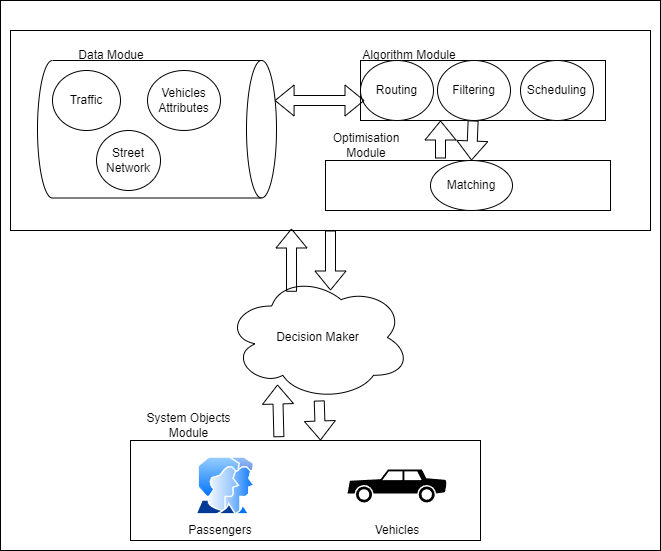
\includegraphics[width=1\textwidth]{Crest/Images/centralised_approach.png}
%     \caption{Centralised Approach to Dynamic Ride-sharing services}
%     \label{fig:centralised_approach}
% \end{figure}

% Since the centralised approach is the prevalent paradigm for handling dynamic ride-sharing problems in the literature discussed, this section discusses its essential components, which are Systems Objects, Data, Algorithms, and Optimisation. 
% The centralised approach places a single-agent decision maker at the heart of the system and includes the following modules: Systems Objects, Data, Algorithm, and Optimisation. Figure \ref{fig:centralised_approach} shows a high-level overview of the centralised approach and how its parts interact in a dynamic ridesharing system. In this strategy, each vehicle connects to a common cloud via the Internet or an intranet to take advantage of the cloud's high-performance computation and vast storage capacity. The cloud holds all necessary resources without duplication, including the street network database and optimisation programme code, among other features, and is in charge of all computations. As shown in Figure 2, when a rider submits a ridesharing request to the system, the system (decision maker) responds after updating the schedules and routes for the appropriate vehicles. The user receives a response that includes the vehicle ID and an expected pick-up time, or a rejection response if the system was unable to match a car to the request.

% \textbf{System Objects Module:}
% A ride-sharing service contains two types of objects: users and vehicles. Users use a mobile or web application to submit real-time requests to the system, which include pick-up and drop-off locations, the number of passengers, a time window for pick-up location, which specifies when the user should be picked up at the origin, and a time window for drop-off location, which specifies when the user should be dropped off at the destination. The latter two sections specify each request's limitations, which must be met in order to solve the ridesharing problem. Moreover, dynamic ridesharing problem must take into account the number of vehicles servicing over a street network (finding a vehicle for each request) by dispatching vehicles with the purpose of minimising or maximising an objective function and satisfying a set of constraints. The fleet of vehicles may vary in capacity and accessibility for certain purposes, such as wheelchair users requesting rides. The cars frequently upload their time-stamped locations to the system, allowing the decision maker to know where each vehicle is at any given time while searching for matches between vehicles and riders.

% \textbf{Data Module:} The database in the Data module contains all the required data for making ridesharing decisions, including a street network (represented as a graph or a grid) for finding routes, traffic data for handling stochasticity about travel times in the street network, and other static and dynamic data about each vehicle such as ID (static), capacity (static), current location and time (dynamic), updated schedule and route for new requests (dynamic), and number of empty seats. The Algorithm module uses the data in this database to conduct a variety of tasks, including identifying best pathways across the network, selecting candidate cars, and changing vehicle schedules when new requests are filed.

% Travel time is critical for routing, and in the absence of traffic data, less reliable routes may be discovered. Incorporating real-time traffic information leads to more optimal routes, but it is computationally expensive \cite{soa_rideshare}, hence most efforts in the literature utilise a pre-computed shortest path technique to solve the time issue. 


% \textbf{Algorithm Module:} This module consists of three submodules: routing, filtering, and scheduling. The routing submodule is in charge of calculating the best travel time between pairs of places on the street network. 


% The purpose of the filtering submodule is to efficiently choose a group of candidate vehicles capable of serving new requests while adhering to the limits of each candidate vehicle's capacity and pick-up and drop-off time windows. Obviously, going through every vehicle locally to match a travel petition when there are a lot of them is computationally unnecessary. To solve this inefficiency issue, spatial data structures such as R-tree \cite{guttman1984rtrees}, KD-tree \cite{bentley1990kdtrees}, R+-tree \cite{sellis1987rplustree}, R*-tree \cite{kriegel1990rtree}, and Quad-tree \cite{bentley1974quadtrees} have been considered. However, these data structures may not be ideal for a large-scale dynamic ride-sharing problem due to the high cost of handling vehicle dynamics and updating indices \cite{xia2003qrtree} \cite{lee2003supporting}.


% \begin{figure}[htbp]
%     \centering
%     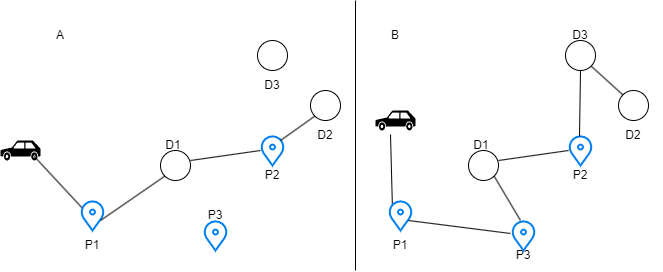
\includegraphics[width=1\textwidth]{Crest/Images/rescheduling.png}
%     \caption{An illustration of rescheduling in a dynamic ride-sharing service. (A) current route of a vehicle for serving two passengers and a new request with pick-up location P3 and drop-off location D3. (B) new route of the vehicle after rescheduling.}
%     \label{fig:rescheduling}
% \end{figure}

% The filtering submodule narrows the search space and selects a set of candidate vehicles. The scheduling submodule is then used to reschedule each vehicle's route and ensure it meets the constraints of the new request and existing rides, such as time windows for pick-up and drop-off locations. In dynamic ridesharing, a ride must begin at the pick-up site and end at the drop-off place. The routing submodule computes the shortest path between each pair of pick-up and drop-off locations. Figure \ref{fig:rescheduling} shows the scheduling submodule in dynamic ridesharing. In panel (A), a vehicle is scheduled to pick up passenger C1 at P1, drop C1 at D1, pick up passenger C2 at P2, and dump C2 at D2. When a new request with the origin P3 and destination D3 arrives, rescheduling is required. Panel (B) depicts the results of rescheduling, a new route, and the order in which passengers are served.

% The rescheduling problem can be addressed in one of two ways: (i) Insert the new request at any point in the current schedule without changing the order of the existing places; this is known as the insertion heuristic approach. To add a new request to the current route with n stops (pick-up and drop-off sites), there are (n+1) (n+2)/2 scheduling options. This method is frequently utilised in the literature \cite{huang2013large} \cite{coslovich2006twophase} \cite{jaw1986heuristic} because to its low computational cost. (ii) create a completely new schedule and solve an open-loop TSP (Travelling Salesman Problem) with a computationally expensive time frame (O(n!)).


% \begin{figure}[htbp]
%     \centering
%     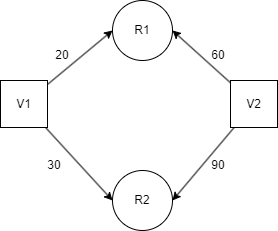
\includegraphics[height=6cm]{Crest/Images/queuing.png} % Adjust the height as needed
%     \caption{An example of queueing approach in ride-sharing problem. The numbers on links are travel times for vehicles-requests \cite{ayala2018spatio}.}
%     \label{fig:queuing}
% \end{figure}


% \textbf{Optimisation Module:}The optimisation module finds an optimal solution to the problem by selecting the candidate vehicle that best meets the request from all of the candidates evaluated by the scheduling submodule for contribution to the objective function. The optimisation module is at the heart of a ride-sharing solution, executing a matching function that assigns vehicles to requests with the goal of optimising an objective function. When determining ride-sharing matches, the models take into account one or a weighted mixture of the following cost functions. \cite{agatz2012optimization}: reducing overall distances or travel times by all cars on the street network; minimising vehicle detours; minimising passenger costs; and maximising the number of successful ride-share requests. These objective functions take into account a range of limitations, including vehicle capacity, user-specified departure or drop-off times, and trip costs. 

% The assignment task is determined by how the optimisation issue handles incoming requests. Essentially, there are two study approaches to addressing the assignment problem: queueing (first-come, first-served) and batch assignment. The queueing strategy, commonly used for solving assignment problems, prioritises all trip requests in chronological order. It should be noted that this is a greedy method that may not produce a global optimal solution because it does not take into account all of the conceivable combinations of shared trip petitions. Using the queuing method shown in Figure \ref{fig:queuing}, request 1 comes before request 2 and vehicles can not handle both at the same time. The optimisation module gives vehicle 1 to request 1, which costs 20, and vehicle 2 to request 2, which costs 90, for a total cost of 110. According to \cite{ayala2018spatio}, this type of vehicle-request assignment matches Nash equilibrium \cite{nash1950equilibrium}. In the scenario in \ref{fig:queuing}, assigning request 1 to vehicle 1 is the best option for vehicle 1 because its travel time to request 2 is longer. Vehicle 2 cannot get request 1 to reduce its trip time because vehicle 1 is closer to request 1. In this case, the vehicles act selfishly for their personal gain rather than attempting to optimise overall performance. While the queuing strategy is effective at tackling the underlying combinatorial optimisation problem, it sacrifices optimality. 

% \begin{figure}[htbp]
%     \centering
%     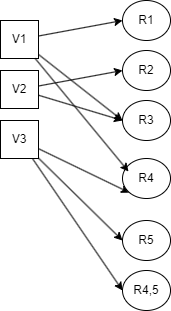
\includegraphics[height=6cm]{Crest/Images/batch_assignment.png}
%     \caption{ An example of batch assignment }
%     \label{fig:batch_assignment}
% \end{figure}

% Figure \ref{fig:queuing} shows that the Nash equilibrium assignment is not optimal. By matching vehicle 2 to request 1 and vehicle 1 to request 2, a better solution with a total cost of 90 is possible. This ideal plan is only possible if incoming requests are aggregated and then allotted to all vehicles within a defined interval. The goal of the batch assignment strategy shown in Figure \ref{fig:batch_assignment} is to compute the optimal assignment of requests to vehicles that minimises or maximises the objective function. Note that each vehicle may be able to handle a group of requests simultaneously; therefore, more nodes will be added to the bipartite graph depicted in Figure \ref{fig:batch_assignment}. Obtaining a close-to-optimal solution in a large-scale dynamic ridesharing situation is the primary rationale for using the batch assignment technique over the queuing strategy, despite the fact that the batch assignment approach is an NP-hard problem. This suggests that heuristics and/or approximate approaches can provide a solution to this large-scale combinatorial optimisation problem in a fair amount of time \cite{liebling1987large}. 

% \subsection{Dynamic Ride-sharing}
% \begin{table}[ht]
% \centering
% \caption{Analogy between dynamic ridesharing problem and different VRP variants.}
% \label{tab:vrp_variants}
% \renewcommand{\arraystretch}{1.5}
% \resizebox{\textwidth}{!}{%
%     \begin{tabular}{|l|c|c|c|c|}
%     \hline
%     \textbf{Problem} & \textbf{Dynamism} & \textbf{Vehicle's capacity} & \textbf{Paired pick-up and drop-off} & \textbf{Time window} \\ \hline
%     \textbf{Dynamic Ridesharing} & \checkmark & \checkmark & \checkmark & \checkmark \\ \hline
%     \textbf{DVRPTW} & \checkmark & \checkmark & & \checkmark \\ \hline
%     \textbf{MTSPTW} & & \checkmark & & \checkmark \\ \hline
%     \textbf{DPDP} & \checkmark & & \checkmark & \\ \hline
%     \textbf{DDARP} & \checkmark & & \checkmark & \checkmark \\ \hline
%     \end{tabular}%
% }
% \end{table}

% \begin{figure}[htbp]
%     \centering
%     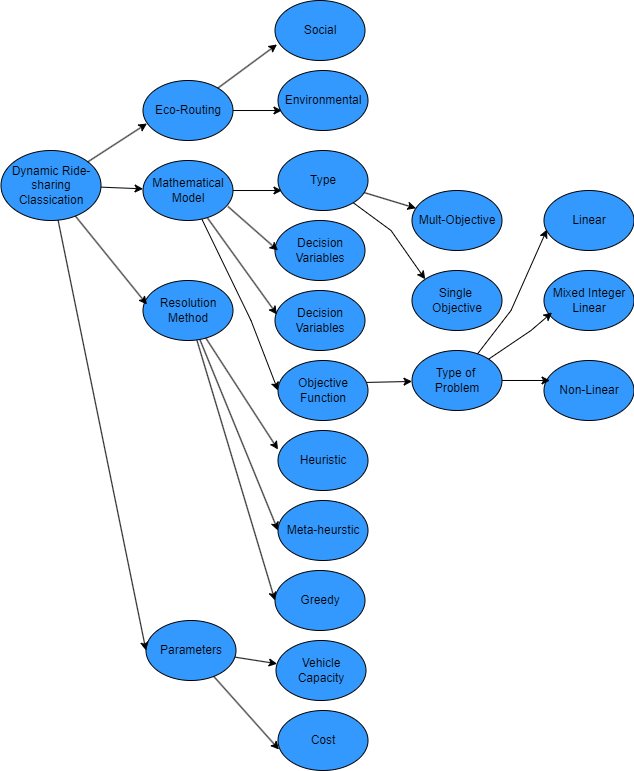
\includegraphics[width=1\textwidth]{Crest/Images/vrp_classification.png}
%     \caption{A systematic review of Dynamic Ride-sharing presented in this literature}
%     \label{fig:vrp_classification}
% \end{figure}

% To further understand the dynamic ride-sharing problem, it is helpful to review prior literature on solutions. The literature on this topic is extensive\cite{Pillac2013DVRPSurvey}, necessitating a focused understanding of the key themes to be addressed when reviewing it. Figure \ref{fig:vrp_classification} presents a systematic overview of these topics, providing a framework for discussion that aligns with the scope of this research. 

% There are several types of solution approaches to the dynamic VRP, including dynamic vehicle routing problem with time window (DVRPTW), dynamic pick-up and delivery problem (DPDP), dynamic dial-a-ride problem (DDARP), and multiple travelling salesman problem with time window (MTSPTW). Table \ref{tab:vrp_variants} compares various kinds of VRP to the dynamic ridesharing problem. It is possible to use the solution to the classic DDARP problem to solve the dynamic ridesharing problem because the two problems are mathematically similar and have similar constraints. These constraints are: a) vehicles with limited capacity; b) passenger requests with a pair of pick-up and drop-off locations; and c) passenger requests with time windows for pick-up and drop-off locations \cite{meng2021dynamic}. The DVRPTW routes begin and stop at a depot, where the concept of pick-up and delivery points is introduced \cite{abdulaal2017solving}. The MTSPTW seeks to find a set of optimal vehicle routes within a certain time frame. In this sort of problem, the concept of dynamism does not exist, the vehicle capacity limitation is released, and, similarly to DVRPTW, the paired pick-up and drop-off site constraint is released \cite{soa_rideshare}. The DPDP approach is appropriate for issues in which requests are made for the delivery of objects such as parcels or letters, time windows are not tight, and capacity limitations do not exist \cite{zhao2021research}. The main idea behind the DDARP is that vehicles start and end their routes at different depots (or the same depot), users' requests are broadcast during the operation, and users must be moved between pairs of pick-up and drop-off locations. The goal is to find the best routes for vehicles that minimise distance while meeting constraints like time windows for each request \cite{thiago19lastmile}. The DDARP allows vehicles to arrive at pick-up sites before the start of the time window but no later than the end of the time window. By example, this holds true for the pick-up and drop-off time windows limitation in the dynamic ridesharing problem. In this context, the dynamic VRP with time windows (DVRPTW) is particularly relevant \cite{meng2021dynamic}. Ride-sharing services must account for dynamic trip requests that arrive in real time, with passengers specifying their pick-up and drop-off times. The system must then allocate vehicles in a way that maximises service efficiency while minimising waiting times and detours\cite{dynamic2024model}. Several factors contribute to the growth of ride-sharing services, including the demand for lower travel costs, concerns about environmental sustainability, and the advancement of connected and autonomous car technologies. Modern ride-sharing services like Uber, Lyft, and BlaBlaCar have proved the power of technology in tackling transportation inefficiencies, but there are still problems in scaling these systems for widespread usage, particularly in urban areas\cite{bakibillah2021incentive}. Adding EVs into the mix introduces further complexity, as the problem must also consider charging schedules and energy consumption \cite{abdulaal2017solving}. Because of the tight relationship between the DVRPTW problem and the DDARP, the remainder of this section focuses on literature that suggest novel techniques for solving variants of the dynamic ride-sharing problem. 

% In \cite{dastpak2021off}, the authors develop a stochastic form of the VRP called the Vehicle Routing Problem with Stochastic Customers and Demands (VRPSCD). In this paradigm, both passenger locations and destinations are unknown at the planning stage. The stochastic information is exposed in two stages: first, customer locations and expected requests are known at the start of the day, and second, actual customer demands are monitored during visits. This challenge is similar to real-world circumstances such as parcel delivery and rubbish collection, in which consumer expectations and locations are unknown until just before service. The VRPSCD's goal is to maximise overall demand supplied within a given time frame, allowing vehicles to return to the depot for preventive replenishment before their capacity is reached. To address this issue, the authors \cite{dastpak2021off} offer a decentralised solution that employs a Markov Decision Process (MDP), allowing vehicles to make autonomous judgements based on real-time data.

% The operational issues of dynamic ride-sharing originate from the engagement of various parties with competing objectives, such as private corporations looking to maximise revenue, governments looking to reduce congestion and pollution, and passengers looking for quick and inexpensive transportation. A greater understanding of the intricate relationships between various parties may result in more successful ride-sharing systems \cite{xie2020optimal} \cite{soa_rideshare}.

% The study \cite{baudru2024comparative} focusses on Peer-to-Peer (P2P) ride-sharing, which leverages private vehicles to pool many passengers with similar itineraries and offers a flexible and low-cost mobility alternative.

% Ride-sharing services can be centralised (big, open groups) or decentralised (small, closed groups), with vehicles owned by one or more ride-sharing participants\cite{houerbi2023blockchain}. Despite ride-sharing's effectiveness in lowering the number of vehicles on the road and associated costs, substantial obstacles persist, particularly in optimising for the preferences of both passengers and drivers \cite{houerbi2023blockchain}. Conflicting aims, such as reducing driving detours and passenger wait times, make it impossible to fulfil all preferences at once \cite{joseph2021blockwheels}.

% This study \cite{baudru2024comparative} compares several strategies for organising ride-sharing groups, including execution time, percentage of satisfied requests, driver detours, and passenger waiting times. The authors present a model to predict user demand based on car usage data from Belgium, allowing them to evaluate multiple user grouping strategies, including OD Similarity, OD Clustering, and Trip Similarity.

% The study emphasises \cite{baudru2024comparative} the economic and environmental benefits of lowering road traffic, stating that inefficient urban mobility costs billions of dollars each year in both the EU and the United States, and that road transport contributes significantly to carbon emissions and urban air pollution. 

% This study \cite{ghandeharioun2023rideshare} examines the operational assignment problem in on-demand ride-sharing services. It aims to model stakeholder objectives and propose policies that provide efficient and mutually beneficial solutions. A real-time simulation framework is created to model dynamic supply-demand matching while accounting for user-specified tolerance times. The optimisation problem is solved with both heuristics and commercial solvers, allowing for quick, efficient decision-making and providing insights into how to improve ride-sharing system operations.



% Dynamic ride-sharing services confront real-time optimisation issues, including the requirement for efficient ride-matching algorithms. In \cite{optimiserideshare}, the authors focus on dynamic ride-sharing from the perspective of sharing cost mechanisms, including uncertainty in trip petitions. Their algorithm assesses various re-optimisation rates, such as when a new trip petition arrives or at predetermined intervals. The method becomes more difficult due to the uncertainty of trip requests, which can be filed anywhere from a few minutes to a few hours before departure. The overall distance travelled or total travel time for each individual ride serve as the optimisation criteria in this scenario. This approach views drivers as private individuals, which means that vehicle availability is linked with their own travel requirements.

% The ride-sharing problem is commonly represented as a Pickup and Delivery Problem with Time Windows (PDPTW), which is known to be NP-hard \cite{nphardness2024wikipedia} \cite{herbawi2012modeling}. The complexity of handling this problem grows with the amount of requests, hence, it is critical to design effective and scalable techniques to handle the high frequency of ride-sharing requests. \cite{zhong2024wait}.

% To overcome the scalability issues in centralised ride-sharing, this work \cite{alisoltani2022spacetime} presents a clustering-based strategy to increase the efficiency and scalability of matching algorithms. The approach provides a "shareability function" (SF) that assesses the likelihood of two trips being shared, taking into account both parallel and sequential sharing possibilities. The SF calculates the additional travel time required to share trips vs serving each trip individually, allowing the clustering algorithm to combine trips with high shareability potential.

% Another study \cite{wallar2019optimizing} proposes a method to estimate the optimal number of vehicles needed to fulfil all travel demand in a city while preserving acceptable waiting times and delays. This offline technique informs fleet operators on the fleet size and vehicle distribution required to fulfil historical demand. The study demonstrates that optimising fleet size and distribution can greatly increase the efficiency of MoD systems, allowing for more effective and strategic fleet management.

% Another key problem is to maintain high service availability. \cite{hafiz2020flexible} focuses on providing real-time scheduling for ride-sharing journeys. They suggest a strategy for reassessing ride-matching over time, clustering passengers and drivers in the same neighbourhood to maximise viable trip options. Their approach ensures a ride back for consumers who have previously received an outbound trip, alleviating concerns regarding trip reliability and return journeys. This ensures a certain level of service quality, as passengers may be confident that once allocated to a journey, they will be able to finish their return trip without further complications.

% Ride-sharing has also been explored as part of multi-modal transportation systems, particularly in last-mile transportation. In \cite{thiago19lastmile} and \cite{zeng2020exploring}, the authors examine dynamic ride-sharing integrated with public transport for the last-mile of a commute. Their work considers the routing of passengers who have reached a central station using public transportation and are now dispersing to their final destinations. The goal is to minimise the number of vehicles on the road by efficiently allocating passengers to available vehicles, thereby reducing congestion and improving travel efficiency.



% Moreover, with the global shift towards sustainable energy, integrating EVs into ride-sharing services has become increasingly important. However, privacy and trust concerns often impede the broader adoption of ride-sharing services. The authors of \cite{Reference4} address these concerns by proposing a co-utilisation framework based on game theory. In their approach, all involved parties must benefit from participating in the ride-sharing service, ensuring mutual trust among passengers and drivers. This framework seeks to reduce travel costs for passengers while also decreasing the number of vehicles on the road and mitigating traffic congestion. Their approach highlights how privacy and trust mechanisms can be integrated into dynamic ride-sharing systems to improve user confidence.

% In summary, while dynamic ride-sharing offers significant benefits, such as reduced congestion, lower emissions, and cost savings, the challenges of real-time optimisation, service reliability, and trust remain crucial to its success. The integration of EVs offers additional opportunities for making ride-sharing more sustainable and widely adopted in urban environments\cite{mamalis2019ridesharing}.

% Eco-routing introduces a variant of DVRP known as Green Vehicle Routing Problem(GVRP). The literature on GVRP is currently developing, with contributions focusing on topics such as reverse logistics, recycling, and emissions management. \cite{lin2014survey} identified research gaps between VRP and Green Logistics, notably the use of time-dependent VRP to reduce emissions during transport. According to studies \cite{salimifard2012green} and \cite{asghari2021green}, integrating environmental costs into VRP is still in its early stages, despite its potential. This work \cite{lin2014survey} adds to the field by doing a comprehensive evaluation of GVRP literature and identifying future research objectives. It provides useful insights for academic studies and practical applications by categorising GVRP variants and exposing gaps in existing research. Governments, non-profit organisations, and corporations can utilise GVRP models to assess the social, environmental and cost implications of transportation plans and take steps towards more sustainable logistics operations. It tries to reduce greenhouse gas emissions and other pollutants produced by transportation systems. It is part of the larger idea of ITS, in which information and communication technology (ICT) plays an important role in optimising different transportation aspects including as speed, route guidance, and traffic signals in order to reduce environmental effect. Eco-routing adds environmental objectives, such as decreasing emissions, whereas traditional vehicle routing models largely focus on minimising journey time \cite{alfaseeh2020multi}.

% Eco-Routing models can be categorised into four aggregation levels\cite{alfaseeh2020multi}:
% \begin{enumerate}
%     \item \textbf{Microscopic (I)}: These models have excellent spatial and temporal resolution, allowing for precise estimations of traffic and emission indicators. However, the trade-offs include longer calculation times, more resource utilisation, and higher input data needs.
    
%     \item \textbf{Macroscopic (A)}: This thesis focusses on macroscopic models that have coarser spatial and temporal resolutions\cite{gridmap}. These models are less precise than microscopic models, but they are easier to use and effective when high-resolution data is unavailable. Macroscopic models are suitable for large-scale situations when simplicity and computing economy are important.

%     \item \textbf{Mesoscopic (E)}: These models strike a balance between microscopic and macroscopic models, with medium levels of spatial and temporal resolution. Despite their potential benefits, none of the reviewed studies applied mesoscopic models for traffic flow and emissions in the context of eco-routing.

%     \item \textbf{Mixed aggregation (M)}: This category includes multiple levels of aggregation for traffic and emission models in order to optimise both.
% \end{enumerate}
% The basic purpose of eco-routing is to steer vehicles along the most energy-efficient routes in order to optimise fuel use and eliminate harmful emissions like GHG \cite{naeem2024energy}. The dynamic End-to-End (E2E) routing system utilises a network of intelligent intersections and CAVs as a famous example of distributed routing. This system uses technologies such as Dedicated Short-Range Communication (DSRC) and 5G to allow for real-time communication between vehicles and infrastructure \cite{djavadian2020multi}. The intelligent junctions collect and communicate real-time traffic data, allowing them to direct CAVs to their destinations while taking into account current network conditions.



% Studies \cite{djavadian2020multi} and \cite{alfaseeh2019multi} have demonstrated that E2E CAV routing systems can reduce travel time and enhance network throughput, especially under high market penetration rates (MPR) and heavy congestion. However, while travel time optimisation alone has shown some potential to reduce emissions, the full benefits of eco-routing may only be realised by explicitly incorporating emission reduction objectives into the routing algorithms. 

% In \cite{ham2021routeoptimise}, the authors present a unique approach to the E-VRP with Time Windows (E-VRPTW) by including Time-of-Use (TOU) electricity pricing, where retail electricity prices fluctuate hourly based on wholesale market circumstances. By intelligently changing vehicle charging to off-peak periods, significant cost reductions can be accomplished. For example, shifting charging from 8 pm to 4 am leads in a 68\% reduction in electricity expenditures. The goal is to reduce not only energy prices, but also the number of EVs utilised and overall journey distance. By incorporating TOU pricing into the E-VRPTW model, this study makes a substantial contribution to cost-efficient routing of electric AV fleets, opening up new possibilities for optimising both transportation and energy management in the developing autonomous taxi business. 

% Heuristics and metaheuristics like genetic algorithms, simulated annealing, and particle swarm optimisation are often used to solve VRP and its variants\cite{kedia2017review}. Exact methods like mixed-integer programming (MIP) are also sometimes used\cite{zuo2017using}. More recent work has explored machine learning-based methods to enhance route optimisation\cite{ren2023solving} \cite{alduoli2018hybridizing}.

% The authors \cite{dastpak2021off} create a Q-learning method, DecQN, to solve the VRPSCD. This reinforcement learning system allows vehicles to learn optimal policies through simulation, and modern techniques such as Replay Memory and Double Q Networks have increased the algorithm's efficiency. DecQN beats benchmark policies for VRPSCD and is competitive with cutting-edge approaches for VRP with Stochastic Demands (VRPSD), despite not being especially designed for that challenge.



% The aforementioned approaches can be used to find solutions to small and medium size 
% instances of the ride-sharing problem in a reasonable amount of time; however, there are some areas for further examination. First, the applicability of the proposed techniques to deal with large-scale 
% optimisation problem with a high degree of dynamism, explained earlier, need to be investigated. 
% Second, in all cases, a queuing approach has been used in serving the new requests; see Section 
% 2.1.4 for a discussion of the pros and cons of this approach. Third, the quality of solutions in these 
% approaches is not known, i.e., how far the objective value of a solution is from the optimal value


% \section{Smart Energy Community based Ride-sharing for Autonomous Electric Vehicles}
% SECs are decentralised energy networks in which local entities (households, companies, and public infrastructure) generate, store, and use renewable energy. These communities rely on distributed energy resources (DERs) such as solar panels, wind turbines, hydro power and battery storage devices to achieve energy independence and sustainability \cite{kahlen2018electric}. SECs are critical to achieving a low-carbon energy future because they optimise local energy production and consumption, reduce reliance on nonrenewable energy sources, and improve grid resilience \cite{vanSummeren2019community}.

% The integration of autonomous electric vehicles (AEVs) into Smart Energy Communities (SECs) has the potential to optimise mobility and energy management \cite{song2023electric} \cite{satoya2014community}. AEVs, as part of shared mobility in Mobility-on-Demand (MoD) networks, can not only meet transportation demands but also contribute to the energy grid using vehicle-to-grid (V2G) technology\cite{dapuzzo2022smart}.The study \cite{kahlen2018electric} found that the mixed rental-trading strategy improves energy markets, fleet owners, and the environment. Integrating EVs into the energy market can lower energy prices by 3.4\%, reduce renewable energy curtailment by 97\%, and enhance earnings for fleet owners by 4.3\%. Sharing transportation services have problems like fleet rebalancing, which happens when EVs gather in areas with high demand at certain times. Adding AEVs that can connect to V2G networks is a way to fix these problems. AEVs have the ability to store excess renewable energy generated by SECs during times of low transportation demand. This allows them to return the energy to the grid when it is required, achieving a balance between the supply and demand of energy. Having this dual capability allows for the optimisation of vehicle availability while also contributing to grid stability through energy redistribution, which ultimately results in a transportation system that is more environmentally friendly and efficient \cite{Reference104}.

% Collaboration between SECs and EV fleets benefits ride-sharing services in particular. By synchronising EV charging with the availability of renewable energy in the community, SECs can ensure that electric vehicles are charged during peak renewable generation periods, such as throughout the day when solar energy is available \cite{piazza2021smartev}. This strategy decreases reliance on fossil fuels for charging and lowers the carbon impact of transport services\cite{fesciogluunver2023electric}. Furthermore, proactive management of EV charging schedules helps to avoid overloading the local grid and ensures that charging occurs when energy prices are lower, increasing the cost-effectiveness of ride-sharing services\cite{wang2016charging} .

% As EV use grows, their batteries can function as distributed energy storage units in SECs. This allows fleet owners to participate in power markets by leveraging spare battery capacity to absorb excess electricity during low consumption periods and discharge it at high demand \cite{spoorthi2022review} \cite{chen2020real}. The paper \cite{vanSummeren2019community} proposes a combined rental-trading model for fleet owners in which EVs are employed for both automobile rentals and energy trading. By treating the fleet as a source of energy, the technique helps optimise when to charge or discharge EVs in response to variable electricity prices.

% The research \cite{kahlen2018electric} collects real-time data on battery levels and EV positions using GSM and GPS. The technique is validated with real-world data from car-sharing fleets in several cities, such as San Diego, Amsterdam, Stuttgart, and Copenhagen. The strategy interacts with Northern Europe's Nord Pool Spot power market, replicating market dynamics as EV fleet owners bid to charge or discharge electricity.


% A significant gap in existing literature is the lack of attention for the variety of charging facilities in EVCSs. In fact, EVCSs often have a variety of charging facilities to satisfy a wide range of customer needs, including slow, regular, and fast charging \cite{afshar2020literature}. This complexity necessitates an effective strategy for optimising the planning of EVCSs with mixed charging facilities.

% The study \cite{luo2018optimal} offers a new optimisation model to minimise the total annualised societal cost of the EV charging system. This cost covers the initial investment, grid reinforcement, operations and maintenance, and network losses. The model uses a Monte Carlo simulation \cite{montecarlo2024wikipedia} to estimate the distribution of charging demands among various types of facilities. To solve the difficult optimisation model, a two-step equivalence and an exact Second-Order Cone Programming (SOCP) relaxation are employed to convert the problem into a Mixed Integer SOCP (MISOCP), which can be effectively solved with commercial solvers.

% Uncoordinated EV charging in an SEC setting may cause grid instability. The study \cite{mao2019energymanage} investigates the potential of smart scheduling strategies to overcome these challenges, avoiding costly infrastructure changes and optimising EV charging to benefit both the power grid and EV users. 

% The study \cite{mao2019energymanage} presents a unique Intelligent Scatter Search (ISS) algorithm architecture to address these difficulties. The ISS framework uses scatter search and sequential quadratic programming (SQP) to manage both unidirectional and bidirectional vehicle-to-grid (V2G) charging scenarios, allowing for variable and steady power rates. This technique is intended to be a complete and universal solution that accommodates a variety of EV charging modes and rates while also meeting current and future smart grid needs.

% Integrating EVs into SECs is crucial for promoting the concept of the "energy citizen." This notion involves people actively engaged in energy generation, use, and management in their own communities \cite{barone2020sec}. Individuals/Communities who own and operate EVs that interact with SECs can help their communities achieve overall energy autonomy while saving money and reducing carbon emissions\cite{boasso2021sec}. This is consistent with broader policy objectives, such as those specified in the European Green Deal, which encourages carbon-neutral cities and sustainable transport networks\cite{greendeal}.

% SECs' decentralised and collaborative concept, along with EV integration, provides a resilient and adaptive infrastructure that is well-suited to the changing demands of modern urban mobility. As cities grow and the transportation sector transitions to electric and self-driving vehicles, SECs' role in promoting sustainable, carbon-neutral transportation systems will become increasingly more important. This collaboration between energy and transport systems marks a big step towards creating smart, sustainable cities capable of meeting the problems of climate change and urbanisation.


\chapter{Carbon-Neutral Community-Based Ride-sharing Framework}
\label{chapter3}

The European Green Deal has set the vision for a climate neutral continent by 2050 \cite{greendeal}.  For transportation systems to meet the aforementioned goal, a sustained transition to mass AEV and a fully RES-based energy market to power them is critical \cite{evplanning}. There is an onus on all citizens to play a role in this green transition; for example,  SECs are emerging to enable distributed energy generation and storage at a local level, representing a step further to the realisation of the term `Energy Citizen' \cite{energydatamanagement}.

Ride-sharing has presented new opportunities for the SEC sector to be productive with energy usage \cite{optimiserideshare}. Dynamic ride-sharing systems aim to match riders and drivers with similar itineraries and time schedules on short notice \cite{soa_rideshare}.
These systems can reduce the number of cars used for personal travel (improving the utilisation of available seat capacity) as well as the total distance for such travels, thus reducing the environmental impact.

The research presented in this chapter includes the design, implementation, and evaluation of a ride-sharing model operating in a smart city containing a number of SECs.

This aligns with the ambition of the EU Green Deal goals, and such a ride-sharing model envisions an alternative carbon-neutral,  community-based,  reactive transportation approach for managing city commutes using autonomous electric vehicles (AEVs).   
It targets  individual citizens (rather than on haulage/commercial transportation) that collectively aim to minimise their impact on the environment through the use of ride-sharing commutes while relying on a fleet of AEVs operating solely on RES. 

Specifically, the chapter includes the following contributions: 
\begin{enumerate}
    \item The formulation of a ride-sharing simulation model with the aforementioned conditions, presented as a variant of the classical Dynamic Vehicle Routing Problem with Time Windows \cite{vrp_survey}.  
    A number of SECs dispersed throughout the city provide the dynamic resources; each of them owns a number of autonomous AEVs and uses its own RES generation function to dynamically charge (and release) them over time. The ride-sharing service serves the dynamic requests provided via TPs, which are released over time. Each TP has its own location and pick-up/drop-off times. The formulation of the ride-sharing model integrates energy generation, allocation, and reactive re-routing constraints, with the objective function of maximising the overall number of TPs being served.  
    \item The design and implementation of the aforementioned ride-sharing model, with an algorithm following a reactive-based simulation approach on top of a greedy-based decision-making process. The algorithm favours scalability over optimality, with the aim for it to be applicable in real-world transportation of large cities. 
    \item The evaluation of the solution approach using a parameterised instance generator. It allows for the fine-grained customisation of (1) a Vehicle Routing Problem-based benchmark and (2) a public transportation-based dataset. Both (1) and (2) are adapted to  the specific requirements and format of the ride-sharing problem, testing the performance and scalability of the algorithm over a number of configurations. 
\end{enumerate}
In summary, this chapter introduces a complete framework for modelling, solving, and analysing a dynamic ride-sharing system powered by decentralised RES. It lays the groundwork for further enhancements in large-scale transportation networks, aiming for both environmental sustainability and operational efficiency.

\section{Mathematical Formulation}
\label{sec:proposed_system}

This section formalises the problem for a carbon-neutral, community-based reactive ride-sharing service as a variant of the classical Dynamic VRPTW. It integrates energy generation, allocation and reactive re-routing constraints as both the TPs and the number of available vehicles evolve during a simulated time horizon.  The ride-sharing service aims to maximise the number of TPs being served.  It is also intended to be highly scalable to facilitate transportation in large cities. 

The ride-sharing service contains the following features:
\begin{itemize}
\item The grid dimensions of the city $c_r$,  $c_c$ and the time horizon for the simulation $th$.  W.l.o.g.,  Manhattan distances among the locations of the city are assumed. 
\[
( c_r, c_c,  tih ) 
\]
\item A set S of SECs, each of them with an id $s_{id}$, a location in the city $s_x$,  $s_y$, a lexicographic-ordered list of the vehicles belonging to it $s_E$, the amount of vehicles ready at the start of the simulation (i.e., at time unit 0) $s_R$ and an energy function $fs_{id}:  \mathbb{N} x \mathbb{N}$ with the energy produced per time unit of the simulation, which will be used to release(in order) each new vehicle from $s_E$ as soon as enough energy to fill its battery capacity is generated. 
\[
( s_{id}, s_x, s_y, s_E,  s_R, fs_{id} ) \forall s\in S 
\]
\item A set E of AEVs, each of them with its own id $e_{id}$, the id of the SEC it belongs to $s_{id}$,  its release time during the simulation $e_{rt}$ (either 0 or when enough energy is generated) and its battery and passenger capacities ($e_{bc}$ and $e_{pc}$).  A mapping from E to S is assumed, such that each $e_{id}$ belongs to one $s_{id}$.
\[
( s_{id},  e_{id},  e_{rt},  e_{bc}, e_{pc} ) \forall e\in Es 
\]
\item A set T of TPs, each of them with its id $t_{id}$, its release time during the simulation $t_{rt}$ and its pick-up (resp. drop-off) locations $ t_{px}$, $ t_{py}$ (resp.  $ t_{dx}$, $ t_{dy}$) and time-windows $ t_{ep}$, $ t_{lp}$ (resp. $ t_{ed}$, $ t_{ld}$).  
\[
( t_{id},  t_{rt},  t_{px}, t_{py},  t_{ep}, t_{lp},  t_{dx}, t_{dy},  t_{ed}, t_{ld} ) \forall t\in T
\]
\end{itemize}

\subsection{Decision Variables}
\begin{itemize}
    \item $Alloc(t_{id}) \in E \cup \{-1\}$: Vehicle assigned to TP $t$, $-1$ if unassigned.
    \item $Sched(e_{id})$: Chronological sequence of movements for each AEV $e$.
\end{itemize}

\subsection{Objective Function}
\begin{equation}
\max \sum_{t \in T} \delta_t
\end{equation}

Where:
\[
\delta_t =
\begin{cases}
1, & \text{if } t_{id} \text{ is served within time windows} \\
0, & \text{otherwise}
\end{cases}
\]

\subsection{Constraints}
Following are the constraints: 
\begin{enumerate}
    \item \textbf{Vehicle Availability:} AEVs are released based on energy generation:    
    \[
    \sum_{t' = 0}^{e_{rt}} fs_{id}(t') \geq e_{bc}, \quad \forall e \in E
    \]
    \item \textbf{Battery Dynamics:} For each movement $m_i \in Sched(e_{id})$:
    \[
    EE_i = ES_i - d(AX_i, AY_i, BX_i, BY_i)
    \]
    Where $d(\cdot)$ is the Manhattan distance.
    \item \textbf{Passenger Constraints:} Pick-ups and drop-offs update $PS_i$ accordingly.
    \[
    0 \leq PE_i \leq e_{pc}
    \]
    \item \textbf{Time Window Satisfaction:} For TP $t$ to be served:
    \[
    t_{ep} \leq TA_{pickup} \leq t_{lp}
    \]
    \[
    t_{ed} \leq TA_{dropoff} \leq t_{ld}
    \]
    \item \textbf{Allowed Movement Types:} \[
    Tl_i =
    \begin{cases}
    +t_{id}, & \text{pick-up for TP} \\
    -t_{id}, & \text{drop-off for TP} \\
    \text{idle}, & \text{vehicle idle period} \\
    \text{ret}, & \text{return to home SEC}
    \end{cases}
    \]
\end{enumerate}

\subsection{Output}
The ride-sharing service is intended to provide an output containing the following features:
\begin{itemize}
    \item A set Alloc, representing an allocation mapping from T to E. 
    \[
    \forall t\in T
    \text{ }Alloc[t_{id}] = 
    \begin{cases}
        e_{id},  \text{if }  t_{id} \text{ is allocated to } e_{id}\\
        -1,  \text{otherwise}
    \end{cases}
    \]
    \item A set Sched, representing a scheduling mapping from E to its sequence of movements (in chronological order) over the entire time horizon. 
    \[
    \forall e\in E
    \text{ }Sched[e_{id}] = ( m_0,  m_1,  \ldots,  m_{n-1} ) 
    \]
    Each movement $m_i$ of a vehicle is represented as
    \begin{align*}
    m_i \equiv \{ ( TA_i, TB,_i AX_i, AY_i, BX_i, BY_i, PS_i, \\
        PE_i, ES_i, EE_i, TL_i, LW_i, TD_i ) \} \\  
    \end{align*}	
    with: 
\begin{itemize}
    \item $TA_i$ (resp. $TB_i$) represent the start time (resp.  end time) of $m_i$. 
    \item $AX_i$ and $AY_i$ (resp.   $BX_i$ and $BY_i$) represent the coordinates of the vehicle at the start (resp. end) of $m_i$.
    \item $PS_i$ (resp. $PE_i$) represents the number of passengers in the vehicle at the start time (resp. end time) of $m_i$. 
    \item $ES_i$ (resp. $EE_i$) represents the battery left in the vehicle at the start time (resp. end time) of $m_i$. 
    \item $Tl_i$ represents a label to identify the purpose of the trip. 
    \begin{itemize}
    \item A movement for picking-up (resp. dropping off) the passenger of $t_{id}$ is marked as $+t_{id}$ (resp.  $-t_{id}$).
    \item An idle movement (resting at a given location) is marked as $idle$. 
    \item A last movement, returning to its home SEC is marked as $ret$.  
    \end{itemize}
    \item $LW_i$ represents the leeway of the movement, i.e., the maximum delay that could be applied to the movement while still accomplishing the action is intended to. 
    \item $TD_i$ represents the movement duration. 
\end{itemize}
\end{itemize}
The proposed carbon-neutral, community-based ride-sharing problem extends the classical DVRPTW, which is well-established as NP-Hard. The additional integration of decentralised SECs, RES generation constraints, battery dynamics, and reactive vehicle scheduling further increases the problem's computational complexity.

Consequently, the category of the problem is NP-Hard. While the current formulation is an optimisation problem aimed at maximising the number of served TPs, a corresponding decision version—determining whether at least $k$ TPs can be served within all constraints—would be NP-Complete, assuming polynomial-time verifiability of candidate solutions \cite{hasan2020commute}.



% \textbf{5. Movement Continuity:}

% \[
% (BX_i, BY_i) = (AX_{i+1}, AY_{i+1})
% \]
% \[
% TB_i = TA_{i+1}
% \]

% \textbf{6. Charging Dynamics at SECs:}

% Battery is replenished at SECs based on available energy $fs_{id}(t)$.


% \subsection{Problem Summary}

% The problem jointly optimises vehicle scheduling, energy allocation, and trip assignments to maximise served TPs, respecting:
% \begin{itemize}
%     \item Energy generation and consumption constraints.
%     \item Passenger capacity and ride-sharing conditions.
%     \item Pick-up and drop-off time windows.
%     \item Geographic vehicle distribution among SECs.
% \end{itemize}

% The resulting system enables scalable, carbon-neutral, community-based ride-sharing under decentralised and dynamic urban conditions.


\subsection{Instance Example}
\label{instance_example}

To highlight the approach taken, an example of a problem instance is presented here. It represents a city of dimensions 3 x 4 (w.l.o.g, 3km x 4km) and a simulated time horizon of 10 units (w.l.o.g., 10 minutes).  
\[
( c_r = 3, c_c = 4,  th = 10 ) 
\]
The city contains just 1 SEC,  with id $SEC_1$ and placed at location (1,2),  with a list of 2 vehicles $S_E \equiv [ AEV_1, AEV_2]$, one vehicle ready to go at the start of the simulation,  and a constant energy generation function of 2kWh per time unit $fSEC_1 = 2$.
\[
 S \equiv \{ ( SEC_1, 1, 2, [AEV_1, AEV_2], 1,  fSEC_1) \}
\]
A constant speed is assumed, making each vehicle to traverse 1 block of the city every time unit, while consuming 1 unit of its battery capacity (w.l.o.g., 60km/h constant speed and 60kWh constant consumption).  
Both AEVs have a battery capacity of 10kWh and room for 5 passengers.  Whereas $AEV_1$ is released at the start of the simulation (time unit 0),  $AEV_2$ is released when its battery capacity is generated by $SEC_1$ (i.e., given the constant energy generation of 2kWh per time unit,  the vehicle is generated at time unit 5).  If $SEC_1$ had had more vehicles in $S_E$, they would have been released (in order) at time units 10, 15, and so on.
\[
E \equiv \{ ( SEC_1,  AEV_1,  0,  10,  5 ),  ( SEC_1,  AEV_2,  5,  10,  5 ) \}
\]
The city receives 3 TPs,  with ids $TP_1$,  $TP_2$ and $TP_3$. 
$TP_1$ is announced at time unit 0,  to pick-up the passenger at location (2,3) between time units 0 and 4, and to drop-off at location (0,0) between time units 5 and 7. 
$TP_2$ is announced at time unit 2,  to pick-up the passenger at location (2,2) between time units 3 and 4, and to drop-off  at location (1,1) between time units 5 and 6. 
$TP_3$ is announced at time unit 6,  to pick-up the passenger at location (2,3) between time units 6 and 7, and to drop-off  at location (1,3) between time units 7 and 9. 
\begin{align*}
T \equiv \{ (TP_1,  ( 0, 2, 3, 0, 0, 0, 4, 5, 7 )), \\
			      (TP_2, ( 2, 2, 1, 1, 1, 3, 4, 5, 6 )), \\
			      (TP_3, ( 6, 2, 3, 1, 3, 6, 7, 7, 9 )) \}		      
\end{align*}
A feasible solution to this instance allocates $TP_1$ and $TP_2$ to $AEV_1$, while $TP_3$ is not allocated.
\[
Alloc \equiv \{ (TP_1, AEV_1),  (TP_2, AEV_1),  (TP_3, -1) \}
\]

In the allocation above,  the vehicles have the following schedules: 
\begin{align*}
Sched \equiv \{ (AEV_1,  [ ( 0, 2, 1, 2, 2, 3, 0, 1, 10, 8, +TP_1, 2, 2 ), \\
									  ( 2, 4, 2, 3, 2, 1, 1, 2, 8, 6, +TP_2, 0, 2 ), \\
									  ( 4, 5, 2, 1, 1, 1, 2, 1, 6, 5, -TP_2, 1, 1 ), \\
									  ( 5, 7, 1, 1, 0, 0, 1, 0, 5, 3, -TP_1, 0, 2 ), \\									 
									  ( 7, 10, 0, 0, 1, 2, 0, 0, 3, 0, ret, 0, 3 )]),\\										 
							(AEV_2,  [ ( 5, 10, 1, 2, 1, 2, 0, 0, 10, 10, idle, 5, 0 )	] \} \\  
\end{align*}							       
	
Figure \ref{fig:sched_instance_example} displays the route of $AEV_1$ and $AEV_2$ in $Sched$. W.l.o.g.,  the coverage of the Manhattan distance between two points is assumed to be traversed always by covering first the distance of the x-axis followed up by the distance in the y-axis.  The release of an AEV is highlighted in blue, an idle movement in grey and an active movement  by its starting point (green) and destination one (red). 
\begin{figure}[b]
  \vspace{-0.2cm}
  \centering
   {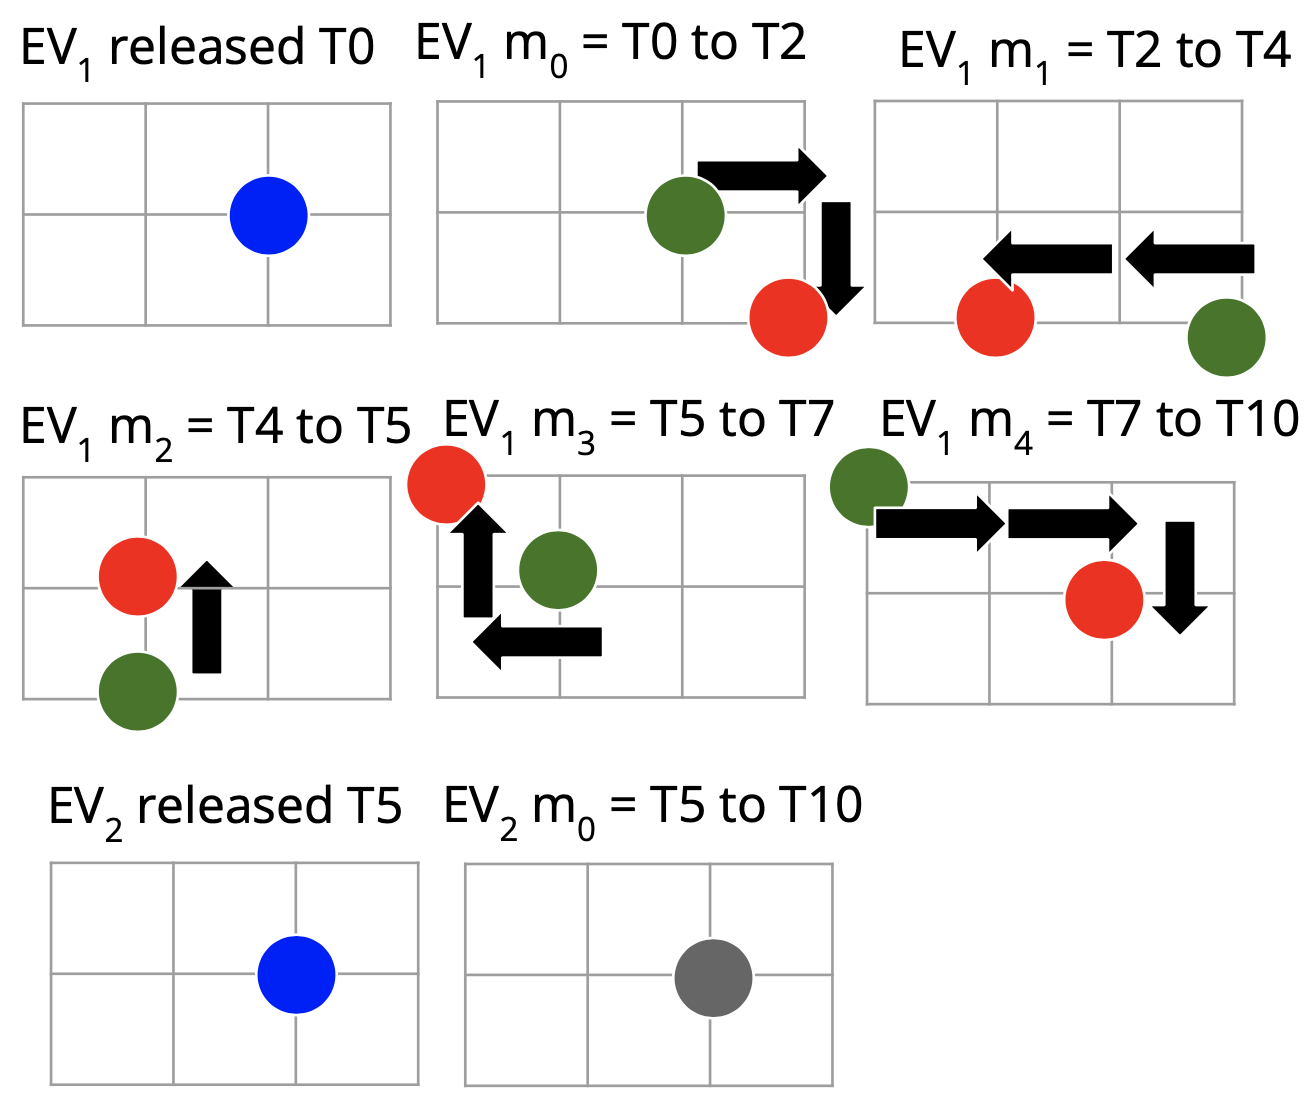
\epsfig{file = Crest/Images/sched.png, width = 0.5\textwidth}}
  \caption{$Sched$ Outputted as Solution}
  \label{fig:sched_instance_example}
    \vspace{-0.1cm}
\end{figure}	
	
The route of $AEV_1$ is composed of 5 movements:									 										 			
\begin{enumerate}
\item From time unit 0 to time unit 2, it leaves the $SEC_1$ to serve the pick-up of $TP_1$.  On doing so,  it goes from (1,2) to (2,3), increases its number of passengers from 0 to 1, and reduces its battery capacity from 10 to 8.  As the pick-up of $TP_1$ must be within time units 0 and 4 and $AEV_1$ arrives at time unit 2,  a leeway of 2 time units is associated to the movement, as it could have been re-scheduled by delaying it up to 2 time units in case the vehicle had needed any re-routing. 
\item From time unit 2 to time unit 4, the vehicle serves the pick-up of $TP_2$.  On doing so,  it goes from (2,3) to (2,1), increases its number of passengers from 1 to 2, and reduces its battery capacity from 8 to 6.  As the pick-up of $TP_2$ must be within time units 3 and 4 and $AEV_1$ arrives at time unit 4,  a leeway of 0 time units is associated to the movement, as it cannot be further delayed by any re-routing.
\item From time unit 4 to time unit 5, the vehicle serves the drop-off of $TP_2$.  On doing so,  it goes from (2,1) to (1,1), decreases its number of passengers from 2 to 1, and reduces its battery capacity from 6 to 5.  As the drop-off of $TP_2$ must be within time units 5 and 6 and $AEV_1$ arrives at time unit 5,  a leeway of 1 time unit is associated to the movement.
\item From time unit 5 to time unit 7, the vehicle serves the drop-off of $TP_1$.  On doing so,  it goes from (1,1) to (0,0), decreases its number of passengers from 1 to 0, and reduces its battery capacity from 5 to 3.  As the drop-off of $TP_1$ must be within time units 5 and 7 and $AEV_1$ arrives at time unit 7,  a leeway of 0 time units is associated to the movement.
\item From time unit 7 to time unit 10, the vehicle returns to $SEC_1$ before the end of the simulation.  On doing so,  it goes from (0,0) to (1,2), stays at 0 passengers, and reduces its battery capacity from 3 to 0.  As the end of the time horizon is at time unit 10, and the vehicle arrives to $SEC_1$ at time unit 10,  a leeway of 0 time units is associated to the movement.
\end{enumerate}

The route of $AEV_2$ is composed of just 1 movement, as the vehicle remains idle since it is released at time unit 5 until the end of the time horizon. 


\section{Solution Approach}
\label{sec:solution_approach:chap2}

This section presents an initial algorithm to solve the problem formalised in Section \ref{sec:proposed_system}.  Subsections \ref{detailed_explanation} and \ref{complexity_analysis} present the algorithm and analyse its complexity, respectively.

\subsection{Algorithm Overview}
\label{detailed_explanation}

Given a valid instance of a city with its SECs, vehicles, energy generation and TPs, the algorithm aims to maximise the number of TPs being served, outputting both the allocation of each trip to a vehicle and the routing of each vehicle over the entire simulated time horizon. To do so, the algorithm implements a reactive simulation approach on top of a greedy decision-making process for trip allocations.  Algorithm 1 presents the pseudocode of the solution approach, which is explained in detail next. 
\begin{algorithm}\captionsetup{labelfont={sc,bf}}
\caption{- Ride-Sharing}
\begin{small}
\begin{algorithmic}
\Function{$allocate$}{$e$, $t$, $Alloc[t]$, $Sched[e]$} 
\State $is\_allocated\gets false$
\State $m \equiv [ m_0, \ldots, m_{k-1} ] \gets copy(Sched[e])$
\For{$i \in 0, \ldots, k-1$}
	\If{$pick\_up(m, t, i)$}
		\State $m\gets [ m_0, \ldots,  m_i', m_{i+1}', \ldots,  m_{r-1}' ]$
		\For{$j \in i+1, \ldots, r-1'$}
			\If{$drop\_off(m, t, j)$}	
				\State $m\gets [ m_0,  \ldots, m_j'',  m_{j+1}'', \ldots,  m_{w-1}'' ]$	
				\If{$ret\_sec(m, w-1)$}
					\State $m\gets [ m_0,  \ldots, m_{w-1}'', m_w'' ]$
					\State $(Alloc[t], Sched[e]) \gets (e, m)$
					\State $is\_allocated \gets true$	
				\EndIf
				\State $Break$				
			\EndIf	
		\EndFor
		\State $Break$
	\EndIf
\EndFor
\Return $is\_allocated$
\EndFunction
\\\hrulefill
\end{algorithmic}
\begin{algorithmic}
\Function{$reactive\_simulation$}{$S$, $E$, $T$, $th$} 
\State $(Alloc, Sched)\gets init(S, E, T, th)$
\For{$t \in sorted(T)$}
	\For{$e \in E$}
		\If{$allocate(e, t, Alloc[t], Sched[e])$}
			\State $Break$
		\EndIf
	\EndFor	
\EndFor
\Return $(Alloc, Sched)$
\EndFunction
\end{algorithmic}
\end{small}
\end{algorithm}



\subsubsection{Reactive-Based Simulation}
\label{reactive_based_simulation}

First, the algorithm initialises $Alloc$, considering each trip as initially not allocated.  It also initialises $Sched$, considering the route of each vehicle as, initially, resting at its home SEC from its release time $e_{rt}$ to the end of the time horizon of the simulation $th$.  
Therefore,  even at the beginning of the simulation (time unit 0), all vehicles have an associated schedule (even if such schedule does not start until a release time unit $e_{rt}$ in the future). 
\[
\forall t\in T\text{ }Alloc[t_{id}] = (e_{id}, -1) 
\]
\begin{align*}
\forall e\in E \text{ } \exists s_{id} \in S \text{ with } s_x, s_y, s_E, e\in s_E \text{ s.t.  } Sched[e_{id}] =\\ 
[( e_{rt}, th, s_x, s_y, s_x, s_y, 0, 0, e_{bc}, e_{bc}, idle, th-e_{rt}, 0 )]
\end{align*}	
For example, given the instance of Section \ref{instance_example}, the initial value of $Alloc$ and $Sched$ is as follows: 
\[
Alloc \equiv \{ (TP_1, -1),  (TP_2, -1),  (TP_3, -1) \}
\]
\begin{align*}
Sched \equiv \{(AEV_1,  [ ( 0, 10, 1, 2, 1, 2, 0, 0, 10, 10, idle, 10, 0 )]\\										 
(AEV_2,  [ ( 5, 10, 1, 2, 1, 2, 0, 0, 10, 10, idle, 5, 0 )] \}\\ 
\end{align*}	

The algorithm then simulates a reactive-based ride-sharing service by simply sorting all TPs by their increasing release time (referred to as $sorted(T)$),  thus attempting to serve each TP as soon as it is released.  For each $t \in sorted(T)$, the algorithm iterates for each $e \in E$, attempting to allocate the trip to the vehicle by dynamically re-routing its schedule (i.e., by fitting both the pick-up and drop-off of $t$ as new movements into the existing schedule of the vehicle $Sched[e]$.  As soon as the algorithm successfully allocates $t$ to a vehicle $e$,  the search stops (i.e., the trip is not attempted to be allocated to any other vehicle). On the other hand, if no vehicle can allocate $t$, then the attempt to serve the TP is considered as not successful, and no further attempt for allocating it is made for the rest of the simulation. 

For example, given the instance of Section \ref{instance_example}, the trips $TP_1$, $TP_2$ and $TP_3$ are released in time units 0,  2 and 6, respectively.  Therefore: 
\begin{enumerate}
\item The algorithm simulates that $TP_1$  is attempted to be allocated first, at time unit 0.  On that moment, the schedule of $AEV_1$ and $AEV_2$ is the initial one described above.  If $AEV_1$ can be successfully re-routed to fit $TP_1$, then it is allocated to it. Otherwise $AEV_2$ is attempted.  If $TP_1$ can not be serviced by either $AEV_1$ or $AEV_2$, then $TP_1$ is not allocated.  In any case, these allocation attempts lead to a new updated state $Sched'$ and $Alloc'$.
\item The algorithm continues by attempting to allocate $TP_2$ over $AEV_1$ first and $AEV_2$ otherwise with their current updated schedules $Sched'$ at time unit 2,  further leading to a new updated state $Sched''$ and $Alloc''$.
\item Finally, the algorithm continues by attempting to allocate $TP_3$ over $AEV_1$ first and $AEV_2$ otherwise with their current updated schedules $Sched''$ at time unit 6, leading to the final state (the one reported as output) $Sched'''$ and $Alloc'''$.
\end{enumerate} 

\subsubsection{TP Allocation}
\label{fitting_into_sched}

The allocation of $t$ to $e$ (specifically, to its schedule $Sched[e]$) is defined to be successful if: 
\begin{enumerate}
\item The updated $Sched[e]'$ incorporates one new movement ensuring the pick-up (resp. drop-off) of $t$ within its defined time window $t_{ep}$ and $t_{lp}$ (resp.  $t_{ed}$ and $t_{ld}$). The functions $pick\_up$ (resp. $drop\_off$) ensure this (cf.  Algorithm 1). 
\item The updated $Sched[e]'$ contains a very last active movement, labelled as $ret$, ensuring the vehicle returning to its home SEC before the end of the time horizon $th$.  The functions $ret\_sec$ ensures this (cf.  Algorithm 1). 
\item The addition of these new pick-up, drop-off and ret movements to $Sched[e]'$ (to serve $t$) might delay the actual pick-up and drop-off times of any other previous trips $t_z$ the vehicle $e$ had previously committed to. For $t$ to be successfully allocated to $e$, such as these additional delays on serving $t_z$ must not break the pick-up and drop-off time windows of $t_z$.  In other words, once a vehicle $e$ commits to a trip $t_z$,  no further trip allocation $t$ can delay $e$ enough to make it not serving $t_z$ in time. The functions $pick\_up$ (resp. $drop\_off$) ensure this (cf.  Algorithm 1).  
\item The updated $Sched[e]'$ contains no movement where the number of passengers exceeds its capacity $e_{pc}$ or where the battery capacity $e_{bc}$ goes below 0. 
\end{enumerate} 

To fit $t$ into $Sched[e] = [ m_0, \ldots, m_{k-1} ]$ 
the algorithm iterates through its movements (which are in chronological order).  When considering a movement 
$m_a \equiv (TA_a, TB_a,  ... )$, the algorithm only considers its starting time unit $TA$ (i.e., the decision of whether to re-route or not $e$ to serve $t$ is considered just at $TA$, not at any other given time in the 
interval $(TA,\ldots,TB]$.  

First, the algorithm searches for a movement $m_i$ fitting the pick-up of $t$.  As soon as such movement $m_i$ is found, no further movement $m_j$ with $j > i$ of $e$ is considered for picking-up $t$, and the algorithm moves on into searching for a movement $m_j$ fitting the drop-off of $t$.  Again, as soon as such movement $m_j$ is found, no further movement $m_k$ with $k > j$ of $e$ is considered for dropping-off $t$.  

Needless to say,  both policies (1) considering just the starting time $TA$ of each movement and the policy (2) considering just one valid pair ($m_{i}$, $m_{j}$) of picking-up and dropping-off movements make the search incomplete. That is, the search is not considering other ($m_{i'}$, $m_{j'}$) valid combinations and any other valid re-routing times for such combinations other than $TA_{i'}$ and $TA_{j'}$. Any such alternatives might lead not only to the allocation of $t$, but to an overall higher number of trips allocated, which is the goal aimed at by the algorithm. However, these policies (1) and (2) are designed to favour scalability over optimality for the algorithm (more detail in Section \ref{complexity_analysis}). 
Moreover, although not leading to optimality, the above non-complete search still leads to a very competitive trip allocation rate when applied to real-world very large instances, as it is discussed in more detail in Section \ref{analysis_performance}.  

Given the instance of Section \ref{instance_example}, the following analyses the attempt to fit $TP_2$ into $AEV_1$ at time unit 2.  
\[
TP_2 \equiv ( 2, 2, 1, 1, 1, 3, 4, 5, 6 )
\]
As described previously,  at this stage in the simulation,  $TP_1$ had been successfully allocated to $AEV_1$, making its $Sched[AEV_1]$:
\begin{align*}
Sched[AEV_1] = [\\ 
m_0 \equiv ( 0, 2, 1, 2, 2, 3, 0, 1, 10, 8, +TP_1, 2, 2 ),\\
m_1 \equiv ( 2, 7, 2, 3, 0, 0, 1, 0, 8, 3, -TP_1, 0, 5 ),\\
m_2 \equiv ( 7, 10, 0, 0, 1, 2, 0, 0, 3, 0, ret, 0, 3 )] 									 
\end{align*}	 

The window of opportunity for allocating the pick-up of $TP_2$ is from $TP2_{rt} = 2$ to $TP2_{lp} = 4$. 

The algorithm first attempts to fit the pick-up on $m_0$, but fails, as the time of the movement $TA_0$ is 0, even before $TP_2$ is announced, and therefore outside of its window of opportunity.  

The algorithm then attempts $m_1$, and it succeeds. $m_1$ spans from time unit $TA_1 = 2$ to $TB_1 = 7$, going from (2,3) to (0,0) for dropping-off $TP_1$.  The total distance covered is 5. It must be at (0,0) at time unit 7 at the latest ($TP1_{ld} = 7$), so it cannot be further delayed.  Re-routing $m_1$ to serve pick-up of $TP_2$ involves (1) going from (2,3) to (2,1); (2) arrive there between time units 3 and 4; (3) going from (2,1) to (0,0); (4) still arrive there on time (i.e., time unit 7 + 0 leeway = 7). The total distance of re-route to pick-up $TP_2$ while still dropping-off $TP_1$ from there is 2 + 3 = 5; if leaving straight-away at time unit 2, it will reach (2,1) to pick-up $TP_2$ at time unit 4, still within the window of opportunity, and leading to a leeway of 0, as this new movement cannot be any further delayed. 

The new state of $Sched'[AEV_1]$ is: 
\begin{align*}
Sched'[AEV_1] = [\\
m_0' \equiv ( 0, 2, 1, 2, 2, 3, 0, 1, 10, 8, +TP_1, 2, 2 ),\\
m_1' \equiv ( 2, 4, 2, 3, 2, 1, 1, 2, 8, 6, +TP_2, 0, 2 ),\\
m_2' \equiv ( 4, 7, 2, 1, 0, 0, 2, 1, 6, 3, -TP_1, 0, 3 )\\ 
m_3' \equiv ( 7, 10, 0, 0, 1, 2, 0, 0, 3, 0, ret, 0, 3 )]										 
\end{align*}	

The window of opportunity for allocating drop-off of $TP_2$ is from the next time unit to its pick-up (5) to $TP2_{ld} = 6$. 

The algorithm first attempts $m_2'$ (as it does not start attempting the drop-off allocation any earlier than the pick-up movement), and it succeeds.  $m_2'$ spans from time unit $TA_2' = 5$ to $TB_2' = 7$, going from (2,1) to (0,0) for dropping-off $TP_1$.  The total distance covered is 3. It must be at (0,0) at time unit 7 at the latest ($TP1_{ld} = 7$), so it cannot be further delayed.  Re-routing $m_2'$ to serve drop-off of $TP_2$ involves (1) going from (2,1) to (1,1); (2) arrive there between time units 5 and 6; (3) going from (1,1) to (0,0); (4) still arrive there on time (i.e., time unit 7 + 0 leeway = 7). The total distance of re-route to drop-off $TP_2$ while still dropping-off $TP_1$ from there is 1 + 2 = 3; if leaving straight-away at time unit 4, it will reach (1,1) to drop-off $TP_2$ at time unit 5, still within the window of opportunity and leading to a leeway of 1 as the time window for dropping $TP_2$ ends at time unit 6 

The new state of $Sched"[AEV_1]$ is: 
\begin{align*}
Sched"[AEV_1] = [\\
m_0" \equiv ( 0, 2, 1, 2, 2, 3, 0, 1, 10, 8, +TP_1, 2, 2 ),\\
m_1" \equiv ( 2, 4, 2, 3, 2, 1, 1, 2, 8, 6, +TP_2, 0, 2 ),\\
m_2" \equiv ( 4, 5, 2, 1, 1, 1, 2, 1, 6, 5, -TP_2, 1, 1 )\\ 
m_3" \equiv ( 5, 7, 1, 1, 0, 0, 1, 0, 5, 3, -TP_1, 0, 2 )\\ 
m_4" \equiv ( 7, 10, 0, 0, 1, 2, 0, 0, 3, 0, ret, 3, 0 )]										 
\end{align*}	

Figure \ref{fig:sched_AEV_1_TP_2} displays the re-routing of $AEV_1$ to fit $TP_2$. 
Whereas its top-left (resp. bottom-left) display the movements before the re-routing for the pick-up (resp. drop-off), the top-right (resp. bottom-right) display the movements after the re-routing.
\begin{figure}[t]
  \vspace{-0.2cm}
  \centering
   {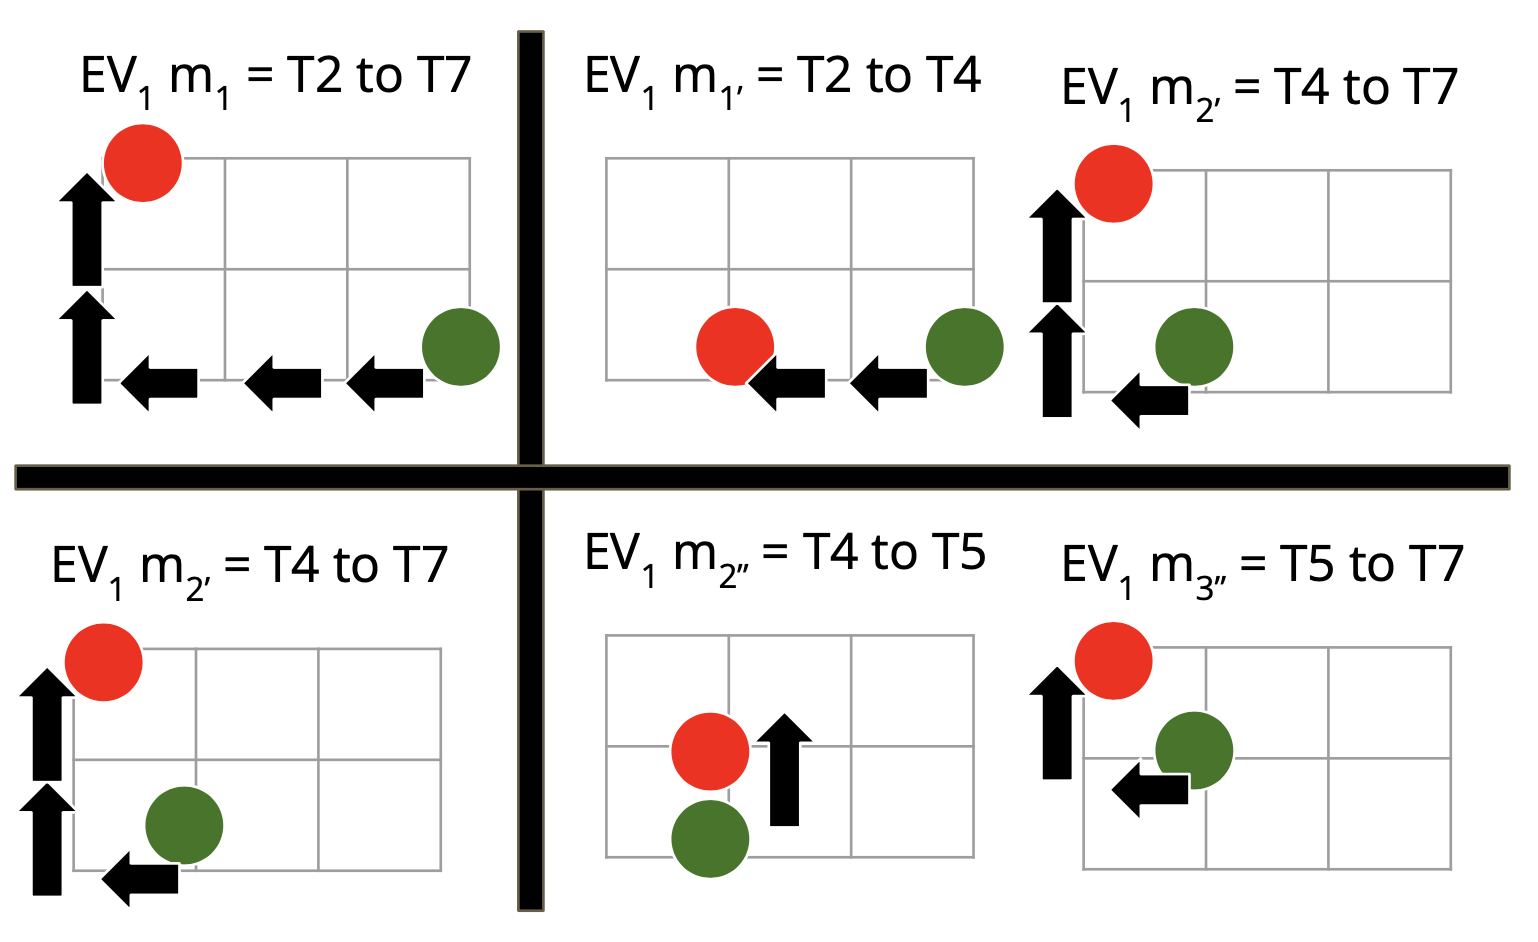
\epsfig{file = Crest/Images/sched_reroute.png, width = 0.9\textwidth}}
  \caption{$Sched[AEV_1]$ when Fitting $TP_2$}
  \label{fig:sched_AEV_1_TP_2}
  \vspace{-0.1cm}
\end{figure}

Finally, if a re-routing movement $m_i$ or $m_j$ serving $t$ implies a delay of $d$ units, this delay must be supported by any further movement in the schedule.  Idle movements use their own leeway to reduce $d$ (until eventually reduce it to 0),  and any other further movement serving $t_z$ must have a leeway of, at least, the remaining delay when reaching it.

\subsection{Complexity Analysis}
\label{complexity_analysis}

An evaluation of the algorithm reveals its complexity to be, at worst, $\mathcal{O}(n^2)$, where $n$ is the number of trips, $m$ the number of vehicles and $n > m$.

%complexity finds it, at worst, to me
%The complexity of the algorithm shows, being $n$ the number of trips, $m$ the number of vehicles, and $n > m$, the worst-time complexity of the algorithm is $\mathcal{O}(n^2)$.

A movement-centric reasoning is used. Given $m$ vehicles, at the start of the simulation each of them has a schedule with a single (very large) idle movement (c.f., \ref{reactive_based_simulation}). From then onwards, each trip is attempted to be allocated, by iterating through the vehicles and, for each vehicle, by iterating through its movements. This means that, in the worst case, first trip will need to explore $m \times 1 = m$ movements. If successful, two new movements will be added to the schedule of the vehicle allocating it (one for pick-up and one for drop-off). Thus, after allocating 1 trip, the overall amount of movements of all vehicles will be $m + 2$ (the $m$ movements being there before and the 2 new ones). The same rationale applies over the next trips attempted to be allocated; for the second trip, a worst-case scenario of $m + 2$ movements will be attempted before allocating it, leading to a new overall amount of $m + 4$ movements, and so on. Given $n$ trips, this leads to an overall amount of 
\[
\sum_{n=0}^{n-1} m + 2n
\]
which can be decomposed as 
\[
\sum_{n=0}^{n-1} m +  \sum_{n=0}^{n-1} 2n = (n m) + \frac{(n^2) - 3n - 2}{2}
\]
 Given that $n > m$, the above expression is dominated by the term $\frac{n^2}{2}$, which leads to a worst-case scenario of $\mathcal{O}(n^2)$.  


\section{Evaluation}
\label{sec:evaluation}

%This section evaluates the carbon-neutral, community-based, reactive ride-sharing service being proposed. 

Section \ref{parameterisable_instance_generator} presents a parameterised instance generator.
%, which is used to customise instances of the Google HashCode'18 challenge (a well-known Vehicle Routing Problem with Time Windows-based benchmark) to the specific requirements and format of the ride-sharing problem defined in Section \ref{sec:proposed_system}.  
The parametric generation enables fine-grained customisation of the instances,  which is then used in sections \ref{analysis_performance} and \ref{analysis_scalability} for respectively analysing the performance and scalability of the solution approach defined in Section \ref{sec:solution_approach:chap2}. 

Then, Section \ref{sec:instances} applies the parametric instance generator to a wider context, in this case customising the well-known, real-world-based dataset of NYC Taxis, for it to fit as valid ride-sharing problem-based instances. This includes a mapping process from the areas and timeline of the original dataset to the grid dimensions and simulation time horizon required by the ride-sharing problem defined in Section \ref{sec:proposed_system}.  The newly generated benchmark is then used in Section \ref{sec:analysis_distance},  analysing the performance of the ride-sharing service from the perspective of the amount of distance covered, as well as from the number of vehicles used compared to (1) more classical taxi-based services or even (2) individual private vehicle transportation-based systems. 

\subsection{Parameterisable Instance Generator}
\label{parameterisable_instance_generator}

Google HashCode \cite{hashcode} is perhaps the most popular team-based programming competition in the world, with more than 100,000 programmers participating on each edition. On the qualification round of 2018, a self-driven-based transportation system (a variant of the classical Vehicle Routing Problem with Time Windows) was proposed as a challenge.  Its very-large complex instances make it an ideal candidate for testing the performance and scalability of the solution approach described in Section \ref{sec:solution_approach}. However, although the challenge was also based on a grid-based city and a simulated time horizon, the following features of the ride-sharing problem described in Section \ref{sec:proposed_system} were not included in the challenge:
\begin{itemize}
\item The model does not include a set $S$ of SECs, nor an ownership mapping from $E$ to $S$. Instead, a single depo at location (0,0) is placed. 
\item The model does not include dynamic availability of requests $T$ and resources $E$ over time. Instead, all vehicles and TPs are available ($e_{rt}$ and $t_{rt}$) at time unit 0.  
\item The vehicles have unlimited battery capacity $e_{bc}$ and room for just one passenger $e_{pc}$. 
\item The pick-up and drop-off windows of the trips contain $t_{ep}$ and $t_{ld}$, but not $t_{lp}$ nor $t_{ed}$. 
\end{itemize}

Therefore, all the above must be incorporated when customising the instances of Google HashCode to the ride-sharing problem.  To enable a fine-grained customisation allowing the solution approach to be tested under different configurations,  an instance generator is implemented, including: 

\textbf{Num SECs.} A configurable integer number of SECs $|S|$ is created across the city, distributed uniformly among its areas.  The vehicles $E$ are also distributed uniformly across $S$, with each $SEC_{id}$ having a same amount of vehicles 
$|s_E|$. 

\begin{figure}[t]
  \vspace{-0.2cm}
  \centering
   {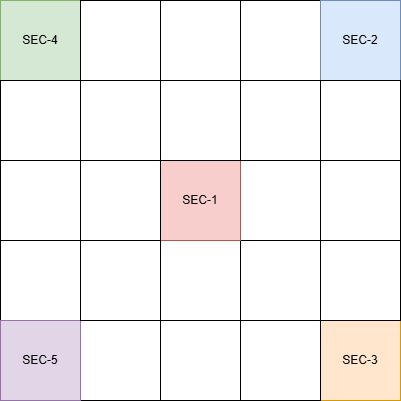
\epsfig{file = Crest/Images/sec_placement.png, width = 0.5\textwidth}}
  \caption{SECs distributed across the grid}
  \label{fig:sched_AEV_1_TP_2}
  \vspace{-0.1cm}
\end{figure}

\textbf{Energy Generation Factor.} Let $sum\_dist$ be the sum of the distance from pick-up to drop-off locations for all trips in $T$.  A float value is passed to specify the $total\_energy$ generated, collectively, by all SECs as a factor of $sum\_dist$. Thus, if factor is 2.0, then $total\_energy = sum\_dist * 2$.  A full use of $total\_energy$ is assumed, as well as its uniform distribution among all SECs and vehicles. Therefore,  the factor ultimately impacts the battery capacity of all AEVs, setting $e_{bc} = \frac{total\_energy}{|E|}$. 

\textbf{Dispatch Mode.} Two vehicle dispatch modes are considered to capture different operational scenarios for SECs in the ride-sharing service. A unique energy generation function $fs$ is assumed to apply to all SECs, determining the availability of AEVs based on energy production.

If $false$ is passed (denoted as $START$ mode), all AEVs of each SEC are released at time unit 0, and $fs = 0$, meaning no further energy is generated after the initial dispatch. This mode simulates scenarios where all SECs begin operations simultaneously with pre-charged AEVs, but no additional RES is produced during the simulation horizon.

Alternatively, if $true$ is passed (denoted as $SPREAD$ mode), a constant energy production rate is set as $fs = \frac{e_{bc} \times |s_E|}{th}$, where $e_{bc}$ is the battery capacity, $|s_E|$ is the number of AEVs per SEC, and $th$ is the time horizon length. In this mode, the first vehicle per SEC is released after time unit 0, while the remaining $|s_E|-1$ AEVs are released gradually, with one new AEV becoming available every $\frac{th}{|s_E|}$ time units.

These two modes are incorporated to evaluate system performance under contrasting conditions: 
\begin{itemize}
    \item The $START$ mode reflects a burst-dispatch scenario, representing systems with fixed schedules or one-time fleet releases.
    \item The $SPREAD$ mode reflects continuous, energy-aware operations, where vehicle availability depends on RES generation distributed across the time horizon.
\end{itemize}
This dual-mode approach enables assessment of the trade-offs between immediate vehicle availability and RES integration in the ride-sharing system.


\textbf{Trip Flexibility Factor.} As discussed, each TP includes $t_{ep}$ and $t_{ld}$, but not $t_{rt}$, $t_{lp}$ nor $t_{ed}$.  In the case of $t_{ed}$, it is simply computed as $t_{ep} + dist$, where dist is the Manhattan distance from pick-up to drop-off location.  A float value between 0 and 1 $flex$ is passed, representing the flexibility percentage for computing $t_{rt} = t_{ep} - (t_{ep}* flex)$ and $t_{lp} = t_{ep} + ((t_{ed} - t_{ep})* flex)$.  If flexibility factor tends to 1.0 (i.e., 100\% flexible), then $t_{rt}$ tends to 0 (early announcement) and $t_{lp}$ tends to $t_{ed}$ (late pick-up far from early pick-up).  In other words, plenty of time to re-route AEVs to accommodate the trip.  On the other hand, if the flexibility factor tends towards 0.0 (i.e., 0\% flexible), then both $t_{rt}$ and $t_{lp}$ tend to $t_{ep}$ (with very little time to react from the announcement of the trip and a very short time window for its pick-up.) 

\subsection{Analysis - Performance}
\label{analysis_performance}

The instance $d\_metropolis.in$ from Google HashCode is selected for its suitability to customise the dynamic ride-sharing problem. This is a large-scale instance, representing a synthetic city of $10,000 \times 10,000$ distance units, a simulation time horizon of 50,000 time units, 400 vehicles, and 10,000 trip petitions (TPs). 

An instance generator is used to fine-tune $d\_metropolis.in$, creating a benchmark set of 72 problem instances, resulting from all possible combinations of the following four parameters:

\begin{itemize}
    \item \textbf{Number of SECs (Num SECs):} $1$, $4$, $16$. A higher number of SECs implies greater geographic and organisational distribution of resources.
    \item \textbf{Energy Generation Factor (EF):} $0.5$, $1.0$, $2.0$. This factor scales the RES production in each SEC, with higher values indicating greater energy availability for vehicle operations.
    \item \textbf{Dispatch Mode (DM):} \texttt{ST} ($START$ mode) or \texttt{SP} ($SPREAD$ mode). In $START$, all AEVs of an SEC are released at time unit $0$, with no further energy production. In $SPREAD$, AEVs are released gradually over time, paced by continuous RES generation.
    \item \textbf{Trip Flexibility Factor (F):} $0.02$, $0.10$, $0.25$, $0.50$. This factor controls the length of time windows for TPs, with higher values indicating more flexible (larger) time windows, and lower values representing rigid time constraints with minimal time to react to new requests.
\end{itemize}

The resulting 72 instances are evaluated using the solution approach detailed in Section~\ref{sec:solution_approach}, with performance measured by the percentage of TPs successfully allocated to AEVs.

A broad range of results emerges from the experimental campaign, with some configurations achieving up to $8,969$ TPs allocated (an $89.69\%$ success rate), while others result in $0\%$ fulfilment.

Notably, the following trends are observed:
\begin{itemize}
    \item Increasing the number of SECs generally improves system performance by enhancing geographic resource distribution and reducing vehicle travel times.
    \item However, this positive effect diminishes or reverses in scenarios with low energy generation factors (EF $= 0.5$). In such cases, having more SECs fragments the limited energy supply across multiple communities, resulting in insufficient energy for vehicle dispatch, and consequently lower TP fulfilment rates.
    \item Greater trip flexibility (higher F values) consistently improves performance, as larger time windows provide more opportunities for vehicle assignment and routing.
\end{itemize}

These interactions highlight the critical balance between infrastructure design (SECs), energy availability, and temporal flexibility in achieving efficient, energy-aware ride-sharing operations.
 
The best configuration is the one with \verb@<@ maximum flexibility, max energy, earlier release of AEV \verb@>@ and, given that the number of SECs might have an impact, the more SECs the better.
\begin{enumerate}
\item[1.] (F - 50\%; SECs - 16; ST; EF - 2.0) $\equiv$  89.69\%
\item[2.] (F - 50\%; SECs - 4; ST; EF - 2.0) $\equiv$ 89.55\%
\item[3.] (F - 50\%; SECs - 1; ST; EF - 2.0) $\equiv$ 82.53\%
\end{enumerate}

The next 3 top results have the same configuration as before, but now with energy factor 1.0.
Therefore, it seems that the best configuration is the one with \verb@<@ maximum flexibility, earlier release of AEV\verb@>@, and given that, the energy factor does have an impact, with the more energy the better. After that, once again, the number of SECs seems irrelevant.
\begin{enumerate}
\item[4.] (F - 50\%; SECs - 1; ST; EF - 1.0) $\equiv$ 77.69\%
\item[5.] (F - 50\%; SECs - 4; ST; EF - 1.0) $\equiv$ 76.95\%
\item[6.] (F - 50\%; SECs - 16; ST; EF - 1.0) $\equiv$ 76.40\%
\end{enumerate}

The next 6 results confirm that, among the duo \verb@<@ maximum flexibility, earlier release of AEV\verb@>@, the earlier release of AEVs seems to be the top factor, as all the 11 top results have START release. But, it can also be observed the crucial importance of flexibility, as by reducing it from 50\% to 25\% the algorithm passes from the previous range of TPs satisfied of [76.40, 89.69] to a reduced performance result of [49.45, 61.84].
\begin{enumerate}
\item[7.] (F - 25\%; SECs - 1; ST; EF - 1.0) $\equiv$ 61.84\%
\item[8.] (F - 25\%; SECs - 1; ST; EF - 2.0) $\equiv$ 61.67\%
\item[9.] (F - 25\%; SECs - 16; ST; EF - 2.0) $\equiv$ 56.26\%
\item[10.] (F - 25\%; SECs - 4; ST; EF - 2.0) $\equiv$ 55.20\%
\item[11.] (F - 25\%; SECs - 16; ST; EF - 1.0) $\equiv$ 51.19\%
\item[12.] (F - 25\%; SECs - 4; ST; EF - 1.0) $\equiv$ 49.45\%
\end{enumerate}

The next 8 results confirm that, among the duo \verb@<@ maximum flexibility, earlier release of AEV\verb@>@, the earlier release of AEVs seems to be the top factor, followed by the flexibility.
If top flexibility is maintained at 50\%, but release the AEVs over the time horizon, the decrease in total TPs satisfied continues, from the previous range [49.45, 61.84] to a new one of [41.73, 49.09].
If flexibility decreases again back to 25\%, then the range decreases even a bit more, to 35.57\% of the petitions satisfied.
\begin{enumerate}
\item[13.] (F - 50\%; SECs - 16; SP; EF - 2.0) $\equiv$ 49.09\%
\item[14.] (F - 50\%; SECs - 1; SP; EF - 2.0) $\equiv$ 48.82\%
\item[15.] (F - 50\%;SECs - 4; SP; EF - 2.0) $\equiv$ 47.76\%
\item[16.] (F - 50\%; SECs - 4; SP; EF - 1.0) $\equiv$ 45.02\%
\item[17.] (F - 50\%; SECs - 16; SP; EF - 1.0) $\equiv$ 42.06\%
\item[18.] (F - 50\%; SECs - 1; SP; EF - 1.0) $\equiv$ 41.73\%
\item[19.] (F - 25\%; SECs - 1; SP; EF - 2.0) $\equiv$ 35.86\%
\item[20.] (F - 25\%; SECs - 1; SP; EF - 1.0) $\equiv$ 35.57\%
\end{enumerate}

The next 16 results show that, all the above analysis state when there is enough energy being produced.
In the case of scarcity of energy, then this turns out to be the most important factor, as the range of TPs satisfied decreases dramatically, to [15.38, 30.31].
That is, if there is a scarcity of energy, the best configuration satisfies the 30.31\% of the TPs.
However, when looking only at SPREAD, there is a configuration leading to 49.09\% of TPs satisfied.
Likewise, when looking only at flexibility 25\%, there is a configuration leading to 61.84\% of TPs satisfied.
\begin{enumerate}
\item[21.] (F - 50\%; SECs - 1; ST; EF - 0.5) $\equiv$ 30.31\%
\item[22.] (F - 25\%; SECs - 1; ST; EF - 0.5) $\equiv$ 29.94\%
\item[35.] (F - 50\%; SECs - 16; SP; EF - 0.5) $\equiv$ 17.07\%
\item[36.] (F - 25\%; SECs - 16; SP; EF - 0.5) $\equiv$ 15.38\% 
\end{enumerate}
The next 24 results show that, all the above analysis state when there is enough flexibility.
If flexibility becomes very low, with the TPs having very little margin (2\% or even 10\%), then the vast majority of the TPs cannot be satisfied, even with an earlier release of AEV and plenty of energy.
\begin{enumerate}
\item[37.] (F - 10\%; SECs - 4; ST; EF - 0.5) $\equiv$ 12.77\%
\item[38.] (F - 10\%; SECs - 16; ST; EF - 0.5) $\equiv$ 12.61\%
\item[39.] (F - 10\%; SECs - 16; SP; EF - 0.5) $\equiv$ 9.95\%
\item[58.] (F - 10\%; SECs - 4; SP; EF - 1.0) $\equiv$ 4.30\% 
\item[59.] (F - 10\%; SECs - 16; SP; EF - 2.0) $\equiv$ 3.93\%
\item[60.] (F - 2\%; SECs - 16; SP; EF - 1.0) $\equiv$ 3.93\%
\end{enumerate}

Interestingly, the lack of flexibility can even lead to 0 TPs satisfied. This is the case when there is just 1 SEC, placed in the centre of the city. Irrespective of the early or spread release of the AEVs, a very tight flexibility in the TPs can make it impossible for an AEV to leave from the centre of the city, and reach both the pick-up and drop-off in time. This situation does not happen at all when there are 4 or even 16 SECs, as this the AEV is closer to extreme pick-up or drop-off points, making it possible to reach to the destination even with a very tight flexibility.
\begin{enumerate}
\item[61.] (F - 10\%; SECs - 1; ST; EF - 2.0) $\equiv$ 0.06\%
\item[72.] (F - 2\%; SECs - 1; SP; EF - 0.5) $\equiv$ 0.00\%
\end{enumerate}

\begin{table}[h!]
\centering
\resizebox{\textwidth}{!}{%
\begin{tabular}{|c|c|c|c|c|c|}
\hline
\textbf{Flexibility (F)} & \textbf{SECs} & \textbf{Dispatch Mode} & \textbf{Energy Factor (EF)} & \textbf{Trips Served (\%)} & \textbf{Observation} \\ \hline
    50\% & 16 & START & 2.0 & 89.69 & Best Overall Performance \\ 
    50\% & 4 & START & 2.0 & 89.55 & High performance with fewer SECs \\ 
    50\% & 1 & START & 2.0 & 82.53 & Impact of centralised SECs \\ 
    50\% & 1 & START & 1.0 & 77.69 & Energy availability effect evident \\ 
    25\% & 1 & START & 1.0 & 61.84 & Flexibility threshold becomes visible \\ 
    50\% & 16 & SPREAD & 2.0 & 49.09 & Delayed vehicle release reduces performance \\ 
    25\% & 1 & SPREAD & 1.0 & 35.57 & Low flexibility combined with delayed release \\ 
    50\% & 1 & START & 0.5 & 30.31 & Severe energy scarcity impact \\ 
    25\% & 1 & START & 0.5 & 29.94 & Energy scarcity + low flexibility \\ 
    10\% & 4 & START & 0.5 & 12.77 & Extreme low flexibility - significant drop \\ 
    10\% & 1 & START & 2.0 & 0.06 & Near-zero TPs satisfied with very low flexibility \\ 
    2\% & 1 & SPREAD & 0.5 & 0.00 & System collapses under tight constraints \\ \hline
\end{tabular}%
}
\caption{Summary of Top Configurations and Key Observations}
\label{tab:config_summary}
\end{table}

The simulation results are summarised in Table-\ref{tab:config_summary}. All in all,  the analysis above leads to the following conclusions: 
\begin{itemize}
\item The most important factor is to have enough flexibility in the TPs (of at least 25\%). Flexibility refers to the length of the time windows associated with each TP. Larger time windows allow for increased scheduling possibilities and more efficient vehicle utilisation. The simulation results reveal a clear threshold effect at $F = 25\%$:
    \begin{itemize}
        \item When $F \geq 25\%$, the ride-sharing service maintains acceptable TP allocation rates (above $49\%$ even under moderate energy constraints).
        \item Reducing $F$ below $25\%$ dramatically decreases performance, with some configurations dropping below $15\%$ TP allocation, even with sufficient energy and optimal vehicle dispatch.
        \item This reflects real-world operational constraints—tight time windows severely limit the system's ability to match AEVs to TPs, especially when geographic distances are large or SECs are sparsely distributed.
    \end{itemize}
The $25\%$ flexibility level thus represents a practical threshold below which the system's efficiency collapses, highlighting the crucial role of designing ride-sharing services that promote or incentivises user flexibility.
\item This is followed by having enough energy (of at least 1.0 times the one required to accomplish all the TPs).
\item With enough flexibility and energy, the most relevant factor is to have earlier release of the AEVs.
\item On top of that, the more flexibility the better (50\% better than 25\%).
\item If all SECs are uniform in terms of their number of AEVs and energy production, then the number of SECs does not have an impact in the results, except for the extreme cases with very few flexibility and a unique SEC placed in the centre of the city.
\end{itemize}
\begin{table}[b]
\begin{center}
\begin{tabular}{|c|c|c|}
\hline
\textbf{Benchmark} & \textbf{Total Time} & \textbf{Avg. Time} \\
\hline
d\_40\_1000 & 40.82 & 0.54\\
d\_100\_2500 & 221.29 & 2.91\\
d\_200\_5000 & 933.2 & 12.28\\
d\_400\_10000 & 9038.0 & 118.92\\
\hline
\end{tabular}
\end{center}
\caption{Scalability of the Algorithm}
\label{scalability_analysis_alg}
\end{table}
\subsection{Analysis - Scalability}
\label{analysis_scalability}

The same 72 instances of the benchmark of Section \ref{analysis_performance} (referred to as $d\_10000\_400$ due to its 10,000 TPs and 400 vehicles) are considered again to evaluate the scalability of the algorithm. 
Also, smaller versions by factor $f$ of such benchmark are achieved by simply removing $\frac{1}{f}$ trips and vehicles from the instances of the original $d\_10000\_400$.  Table \ref{scalability_analysis_alg} shows the total running time (resp. average running time per instance) in seconds as the size of the instances scale from 1,000 trips and 40 vehicles to 10,000 trips and 400 vehicles.  Benchmarks have been run in a Mac OS Ventura, Intel i7 Quad Core 2.3Ghz processor
and 16GB RAM memory.  The algorithm has been implemented in Python and run with Python 3.10.5. 

The results confirm the scalability of the solution approach of Section \ref{sec:solution_approach}, as it is able to solve very large instances (as the ones of $d\_10000\_400$) in less than 2 minutes.  Together with the previous analysis in Section \ref{analysis_performance}, it is concluded that the algorithm provides both good performance and scalability.  


% ------------------------------------
% NYC Taxis
% ------------------------------------
%\input{content/05_1_experimental_setup}

\subsection{NYC Taxi Instances}
\label{sec:instances}

The dataset covers the entire fleet of taxi operators in NYC and comprises a total of 1,048,575 trips \cite{nyc_data}. The records include fields to capture pick-up and drop-off dates/times, pick-up and drop-off locations and trip distances. The data used were collected and provided by the NYC Taxi and Limousine commission by technology providers authorised under the Taxi cab and Livery management enhancements program. The NYC taxi data models a wide array of attributes such as \textit{tip\_amount}, \textit{payment\_type}, and \textit{fare\_amount}. However, for the experiments conducted, the attributes considered are mentioned in Table \ref{tab:nyc_ex}.
\begin{table}[b]
\centering
\begin{tabular}{|c|c|}
  \hline
   \textbf{Attribute} & \textbf{Eg.Value} \\
  \hline
   \textit{!pep\_pickup\_datetime} & 01/01/2018 12:18:50 AM \\
  \hline
    \textit{!pep\_dropoff\_datetime} & 01/01/2018 12:24:39 AM \\
  \hline
   \textit{PULocationID} & 236 \\
  \hline
    \textit{DOLocationID} & 236 \\
  \hline
    \textit{trip\_distance} & 0.7 \\
  \hline
\end{tabular}
\caption{NYC Attributes}\label{tab:nyc_ex} 
\end{table}

The ride-sharing model allows various vital parameters to be dynamically adjusted, as presented in Section \ref{parameterisable_instance_generator}. 
On top of the configuration described then, the customisation of the NYC taxis uses a fixed battery capacity per vehicle, and then allows to parameterise the total amount of vehicles as a factor of such battery capacity and the total energy being produced. 

\subsubsection{Grid-generation}
A grid-based mapping approach is used. This approach significantly decreases the time required to analyse data compared to a spatial resolution of near-continuous coverage data \cite{gridmap}. Grid-based mapping provides a consistent and standardised approach to spatial data collection. A grid map is a set of cells where the users can customise their geometries, and visual representations \cite{nyc_geo_study}. An example of a grid map of taxi zones in NYC is shown in Figure \ref{fig:attributes_grid}.
To divide the spatial polygon of the NYC map with 262 taxi zones \cite{nyctaxi} into a grid, Quantum Geospatial Information System (QGIS) used.
The OGC coordinate reference system (OGC: EPSG7326-WGS84), proposed in the world geodetic system 1984 ensemble (EPSG:7326), is used to form the grids. The average trip distance from the NYC taxi data set is 4.32km, with the shortest trip being 0.32 km. Therefore, the horizontal and vertical spacing is set at 0.016 km, and a `\textit{420X556}' grid map is generated. A  GeoJSON file is generated for the grid layout of the NYC map. The instance generator computes the pick-up and drop-off locations of passengers based on the `\textit{PULocationID}', the `\textit{DOLocationID}' and \textit{trip\_distance} of the passengers from Table \ref{tab:nyc_ex}.
\begin{figure}[t]
  \vspace{-0.2cm}
  \centering
   {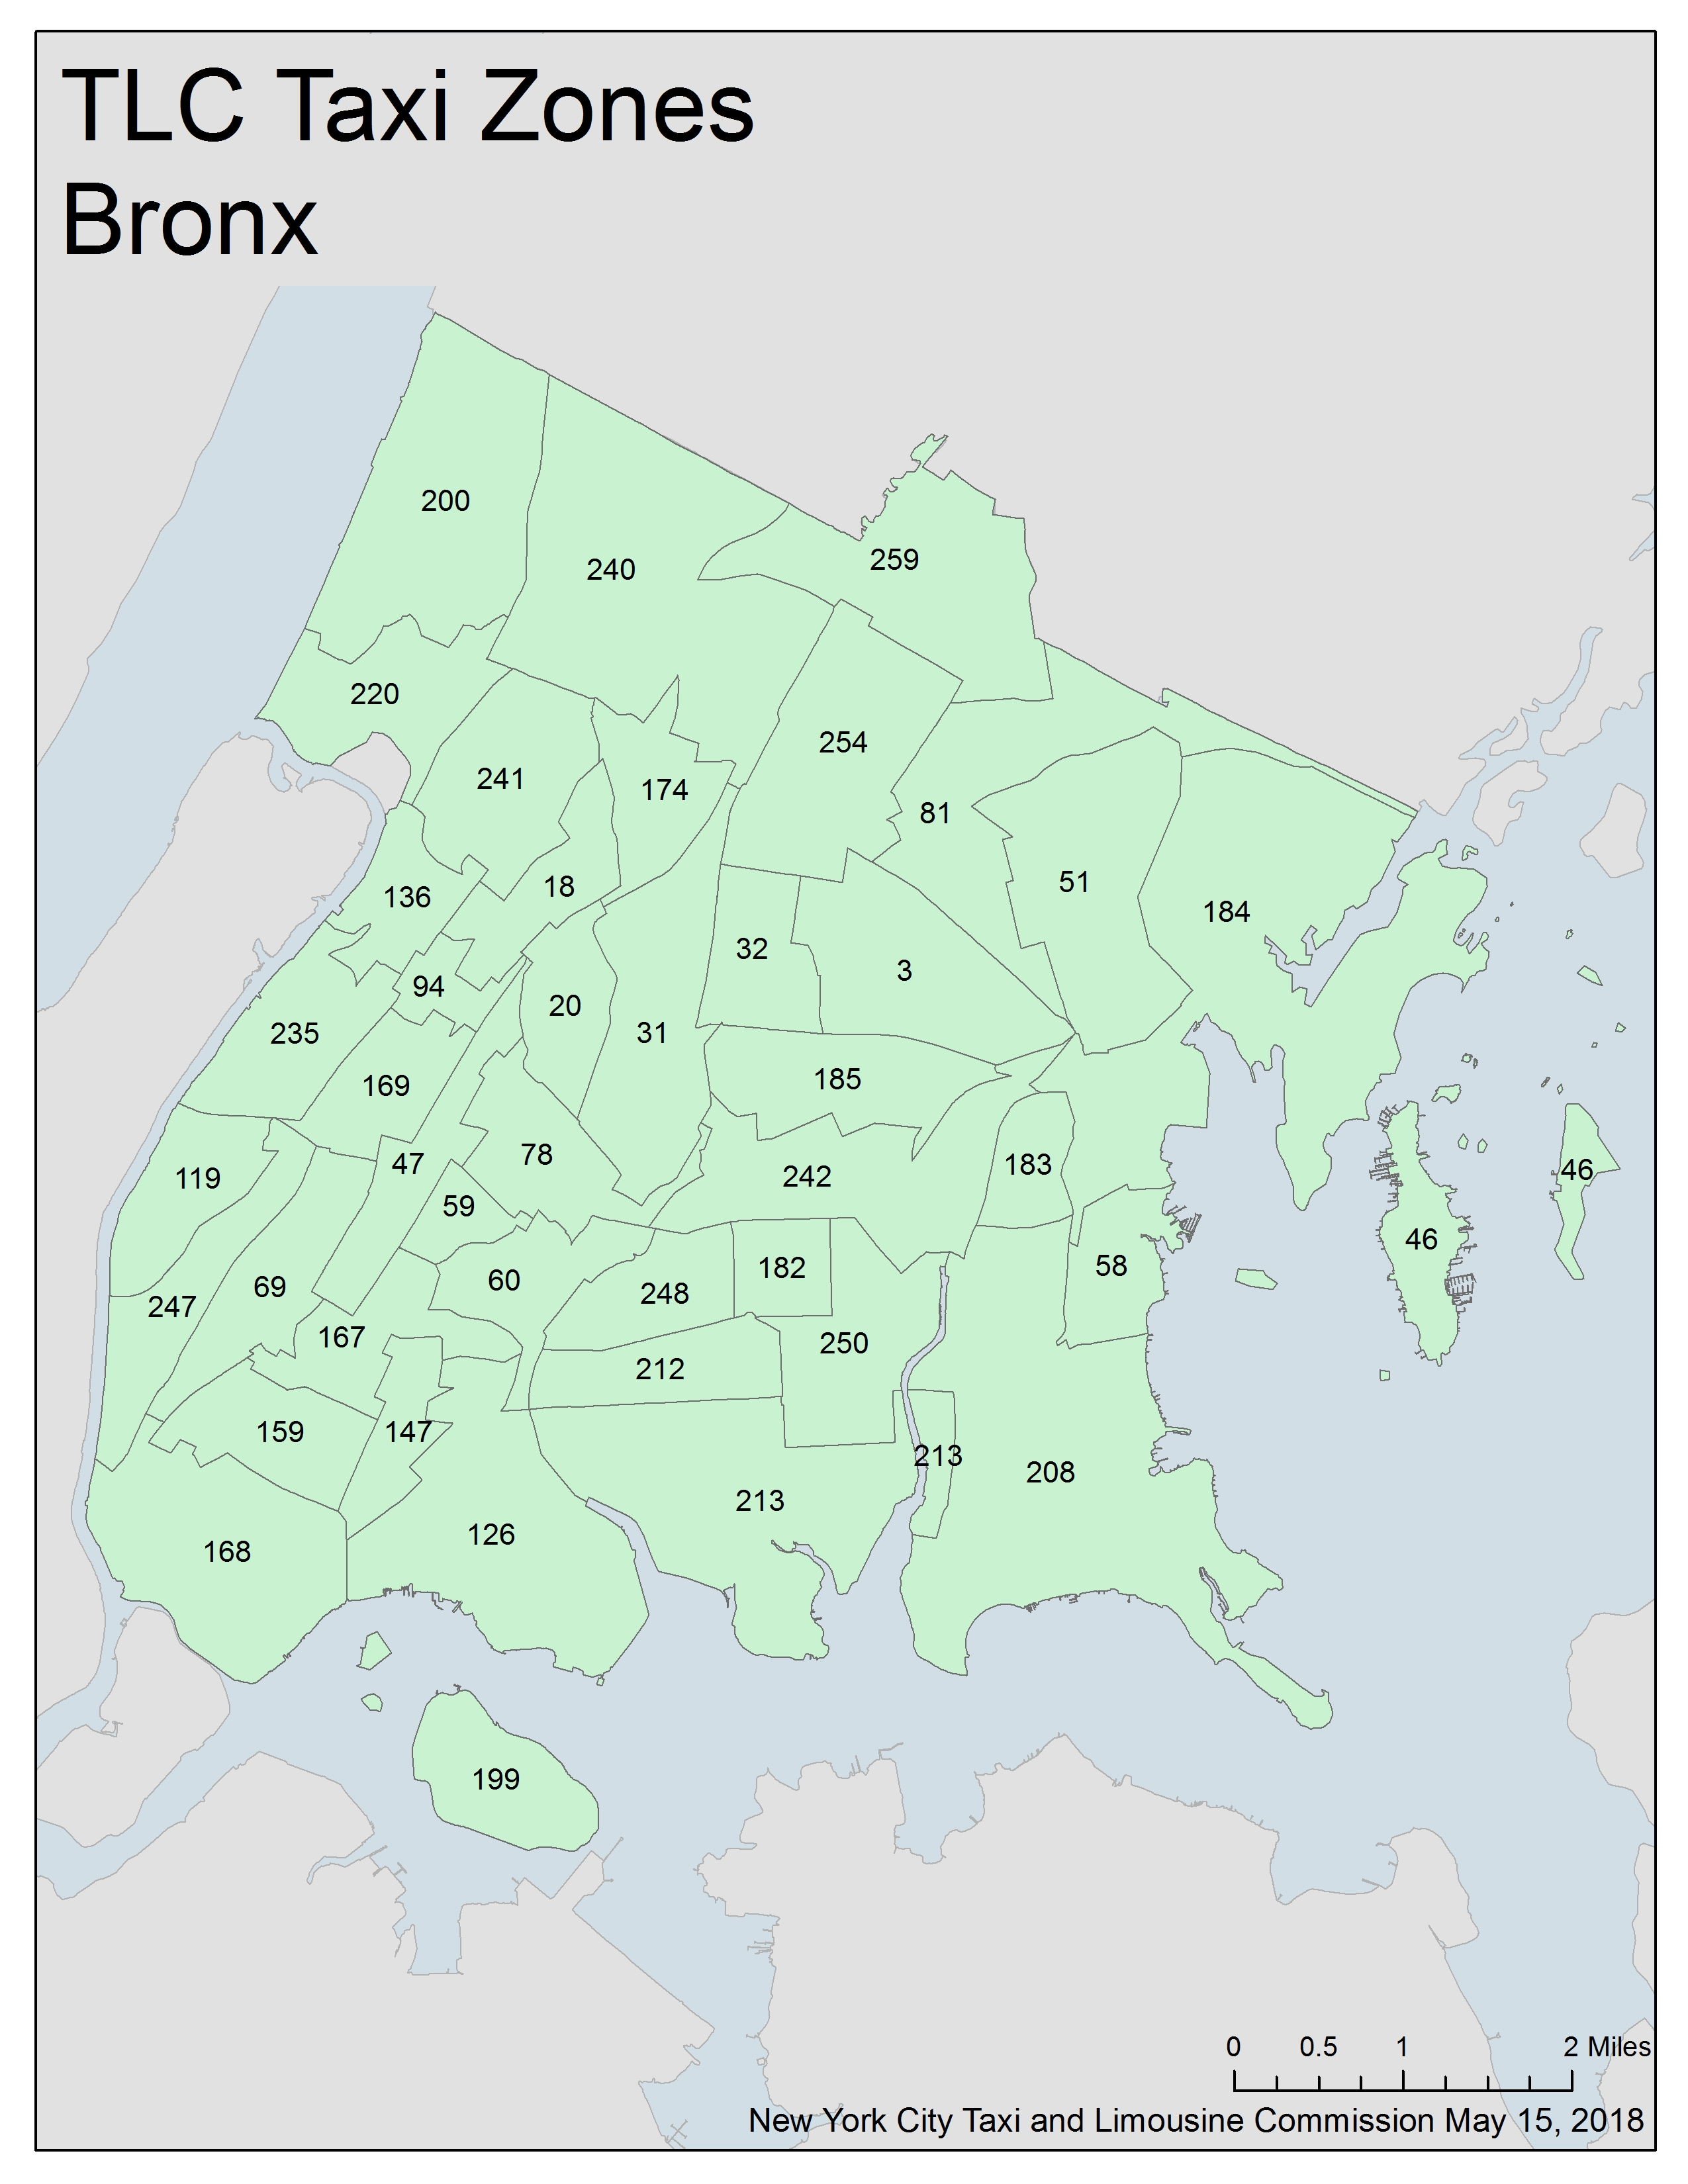
\epsfig{file = Crest/Images/taxi_zone_map_bronx.jpg, width = 5.5cm, height = 4.5cm}}
   \caption{Taxi zones in Bronx, New York \cite{nyc_data}}
    \label{fig:attributes_grid}
  \vspace{-0.1cm}
\end{figure}

% ------------------------------------
% Analysis - Number of Vehicles and Distance
% ------------------------------------

\subsection{Analysis - Ride-sharing vehicles and Distance Traversed}
\label{sec:analysis_distance}

Interestingly, when evaluating the ride-sharing service on a large-scale real-world dataset—specifically the NYC taxi data—the optimal parameter configuration was found to be identical to the one identified in Section \ref{analysis_performance}. This configuration:
\[
(F - 50\%; SECs - 16; ST; EF - 2.0) 
\]
consistently yielded the best performance in terms of [insert your metric: e.g., minimised total cost, highest ride-matching rate, or another objective]. This result reinforces the robustness of the earlier analysis and suggests that the previously derived configuration is not only effective in controlled scenarios but also scalable and reliable in real-world applications.

This time, the experiments are focused on analysing the performance of the ride-sharing service when compared to both a more classical taxi-based service and an individual, private vehicle transportation-based model. Both the amount of distance covered and the number of vehicles used are analysed.
\begin{itemize}
\item \textbf{Taxi Mode}: In this mode, AEVs aim to pick-up and drop-off passengers sequentially, as opposed to the ride-sharing  mode, where several passengers might, temporarily, share a vehicle during their trips. 
\item \textbf{Individual Mode}: This mode represents a private mode of transportation. Each passenger uses a privately owned AEV to commute from the pick-up to the drop-off point.  
\end{itemize}

The extra distance the AEV must travel from the drop-off point to the pick-up point of subsequent requests is what determines the overhead of both taxi and ride-sharing modes in comparison to individual mode. Whereas in ride-sharing mode the possibility of having multiple passengers sharing the vehicle  might reduce this extra distance, in the case of the taxi mode the extra distance becomes non-avoidable. 

% \begin{table}[h]
% \centering
% \begin{tabular}{|c|c|c|}
%  \hline
%   \textbf{Mode} & \textbf{Vehicles} & \textbf{Distance(km)} \\
%  \hline
%    Ride-share & 704 & 112575 \\
%  \hline
%    Taxi & 718 & 153862.4  \\
%  \hline
%   Individual & 4514 & 92654 \\
%  \hline
% \end{tabular}
% \caption{Ride-share vs Taxi vs  Individual}\label{tab:comparision} 
% \label{last_table}
% \end{table}

Table \ref{last_table} shows the results 
when running a large instance with thousands of TPs. The ride-sharing service is configured to use 704 vehicles, and it manages to serve 4,514 TPs. When compared to individual mode, 
the use of the ride-sharing service would have allowed to put 4,514 - 382  = 4132 vehicles out of the road, a reduction of an 84.4\%. 
\begin{table}[b]
\centering
\begin{tabular}{|c|c|c|}
 \hline
  \textbf{Mode} & \textbf{Vehicles} & \textbf{Distance(km)} \\
 \hline
   Ride-share & 704 & 112575 \\
 \hline
   Taxi & 718 & 153862.4  \\
 \hline
  Individual & 4514 & 92654 \\
 \hline
\end{tabular}
\caption{Ride-share vs Taxi vs  Individual}\label{tab:comparision} 
\label{last_table}
\end{table}

% The algorithm is then re-run for taxi mode. This time it is set to contain:
% only the 4,514 petitions that were served above; 
% an unlimited amount of vehicles  (to ensure that all 4,514 trip petitions are indeed satisfied);
% and a single passenger capacity on each vehicle (to ensure that no two trip petitions might share a vehicle while being served). 
% The focus is now on the actual number of vehicles used by the algorithm, which turns out to be slightly higher than before (718, an increase of 46.79\% w.r.t. ride-sharing mode). 

% In terms of the overall distance traversed, the ride-sharing mode has an overhead of 112575 - 92654 = 19,921 extra kilometers, representing an increase of 21.5\% in the distance on the individual mode. In the case of taxi-mode, this increase is even higher 113862.4 - 112575 = 1287.4km, confirming the benefits of the ride-sharing mode vs. the taxi simulation also. 

The algorithm is then re-run for taxi mode. In this simulation, it is configured as follows:
\begin{itemize}
    \item Only the $4,514$ TPs previously served in ride-sharing mode are considered.
    \item An unlimited number of vehicles is permitted, ensuring that every TP can be satisfied individually.
    \item Each vehicle has a single-passenger capacity, preventing multiple TPs from sharing a vehicle.
\end{itemize}

The focus of this experiment is on evaluating the number of vehicles required and the overall distance traversed. The results show that $718$ vehicles are needed to satisfy all $4,514$ TPs in taxi mode, compared to $704$ vehicles required in ride-sharing mode. This represents an increase of $1.99\%$, a relatively modest difference.

At first glance, the small increase in the number of vehicles raises some concerns about the effectiveness of ride-sharing. In theory, ride-sharing should drastically reduce the number of vehicles required by allowing multiple passengers to share rides simultaneously. The fact that taxi mode only needed $1.99\%$ more vehicles suggests either that the average occupancy rate in ride-sharing mode is close to one passenger per vehicle at a given time or that the TPs had substantial time flexibility, making it easier for vehicles to serve sequential trips without overlapping rides. In either case, this result indicates that the advantages of ride-sharing, purely in terms of vehicle count reduction, are limited under the given conditions. Therefore, from a vehicle usage perspective alone, this outcome is less favourable to the ride-sharing mode than initially expected.

However, a more positive picture emerges when analysing the overall distance traversed by the fleet. In individual mode, the total distance traversed is $92,654$ km. In ride-sharing mode, this increases to $112,575$ km, representing a $21.5\%$ overhead compared to individual transportation. Meanwhile, in taxi mode, the distance rises further to $153,862.4$ km. This means that taxi mode results in an additional $41,287.4$ km travelled compared to ride-sharing mode.

Thus, even though the number of vehicles required is similar between taxi and ride-sharing modes, ride-sharing achieves a better optimisation of distance travelled. The fact that taxi mode requires more distance to serve the same number of TPs highlights the efficiency of ride-sharing in route combination and dynamic scheduling. 

In conclusion, while the experiment demonstrates that ride-sharing does not greatly reduce the number of cars compared to taxi mode, it does significantly lower the overall distance travelled, which is helpful in terms of energy usage and traffic congestion.  This demonstrates one of the main advantages of the proposed ride-sharing paradigm.


\subsection{Analysis- AEV Dispatching Strategies}
\label{sec:ev_dispatching_strategies}

To further evaluate the proposed ride-sharing model's performance, experiments are carried out with the best configuration reported in Section 3.3.2 for the instanced from Google HashCode.
\[
     (F - 50\%; SECs - 16; ST; EF - 2.0) \equiv  89.69\%
\]

Specifically, the performance of two dispatch methods are compared:

\begin{itemize}
    \item \textbf{START:} All AEVs are released at the beginning of the simulation.
    \item \textbf{SPREAD:} Vehicles are gradually deployed over the simulation time horizon.
\end{itemize}

The goal of this experiment is to evaluate how vehicle release times affect performance indicators such as trip satisfaction, energy consumption, and idle time in AEV.

The simulation is run for both dispatch modes under varying energy generation rates. The following key metrics are recorded for each mode:
\begin{itemize}
    \item \textbf{Time to Serve First TP:} Time required to service the first trip after the simulation begins.
    \item \textbf{Average Trip Satisfaction Rate:} Percentage of TPs successfully allocated to vehicles over the course of the simulation.
    \item \textbf{Energy Consumption Patterns:} Total energy consumed by the AEV fleet during the simulation.
    \item \textbf{Idle Time:} Duration during which AEVs were idle (i.e., not serving any TPs).
\end{itemize}

\subsubsection{Results and Analysis}

% \paragraph{Time to Serve First Trip Petition:}
Figures~\ref{fig:first_trip_time} and Table~\ref{tab:first_trip_time} illustrate how the average time taken to serve the first TP by newly activated AEVs evolves throughout the simulation.

At each simulation step, new vehicles become available (in SPREAD mode), or all vehicles are already available (in START mode). The value recorded at each step represents the average reaction time, defined as the time difference between a trip being announced and the first successful allocation of a vehicle to serve it. Thus, this is not the time to serve the very first global petition but the average service time observed among vehicles becoming active during that window.

In the START mode, the time to serve TPs is consistently lower throughout the simulation since all vehicles are deployed from the beginning, maximising responsiveness. In the SPREAD mode, the time to serve trips gradually decreases as more vehicles are progressively deployed, although it remains higher than in the START mode.

\begin{figure}[h!]
    \centering
    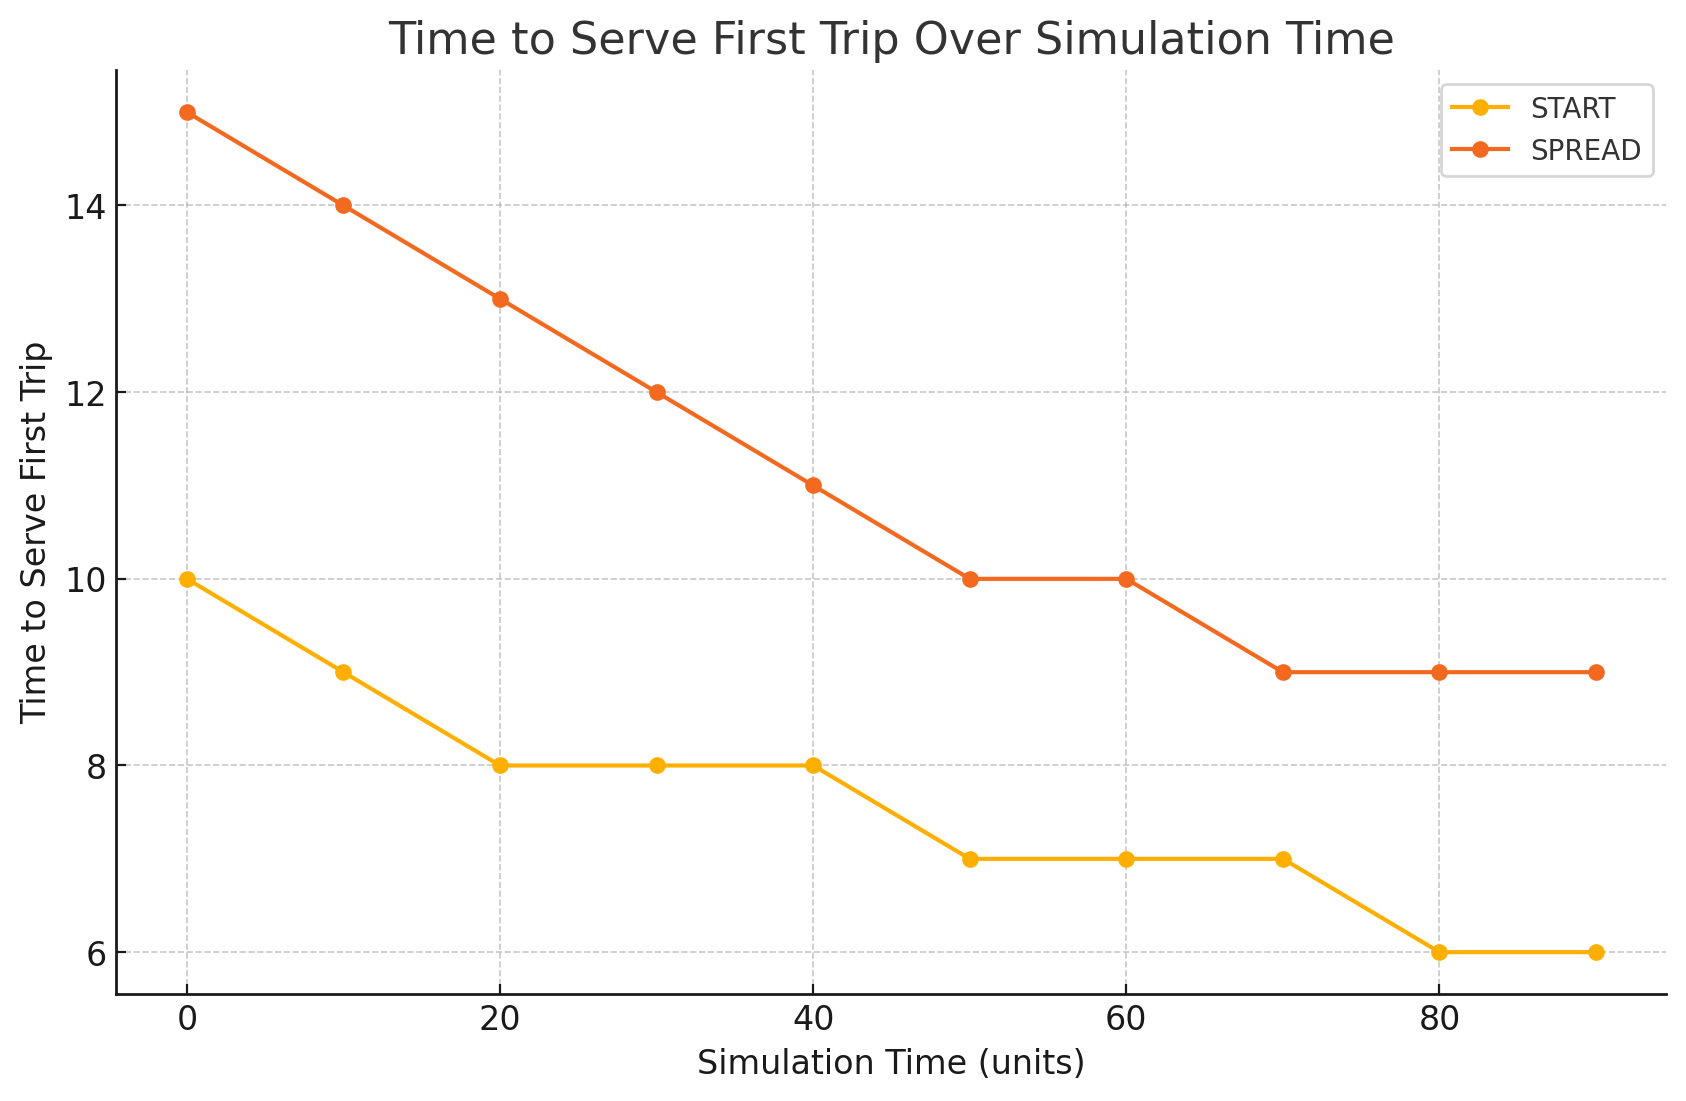
\includegraphics[width=0.8\textwidth]{Crest/Images/first_trip_time.png}
    \caption{Average Time to Serve the First TP for Newly Activated Vehicles over Simulation Time}
    \label{fig:first_trip_time}
\end{figure}

\begin{table}[h!]
\centering
\begin{tabular}{|c|c|c|}
\hline
\textbf{Simulation Step(\%)} & \textbf{START Mode} & \textbf{SPREAD Mode} \\ \hline
0  & 10 & 15 \\ 
10 & 9  & 14 \\ 
20 & 8  & 13 \\ 
30 & 8  & 12 \\ 
40 & 8  & 11 \\ 
50 & 7  & 10 \\ 
60 & 7  & 10 \\ 
70 & 7  & 9  \\ 
80 & 6  & 9  \\ 
90 & 6  & 9  \\ \hline
\end{tabular}
\caption{Average Reaction Time to First TP by Newly Activated Vehicles under START and SPREAD Dispatch Modes}
\label{tab:first_trip_time}
\end{table}

% \paragraph{Trip Satisfaction Rate:}
Figure \ref{fig:satisfaction_rate} and Table \ref{tab:satisfaction_rate} demonstrate that the rate of TPs being served for the START mode is greater early in the simulation due to the quick availability of AEVs. However, both approaches converge with time, with the SPREAD mode reaching a similar satisfaction rate at the end of the experiment.

\begin{figure}[h!]
    \centering
    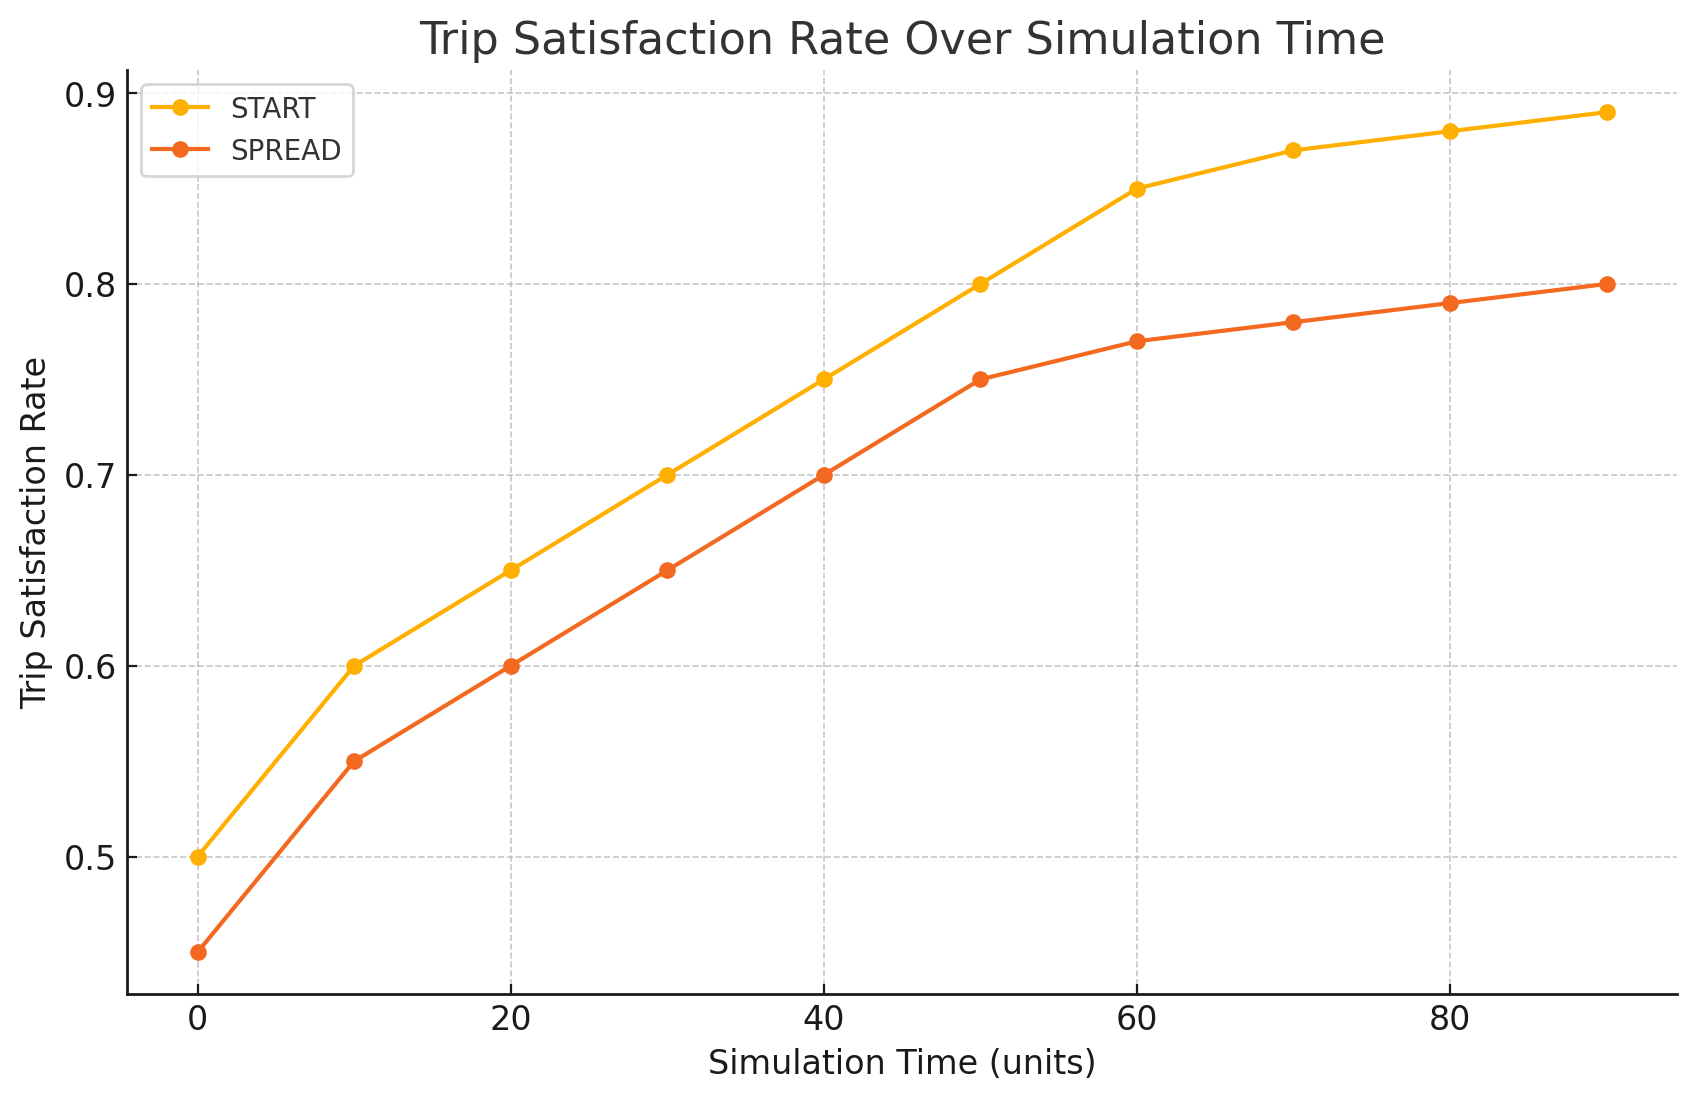
\includegraphics[width=0.8\textwidth]{Crest/Images/satisfaction_rate.png}
    \caption{Trip Satisfaction Rate Over Simulation Time}
    \label{fig:satisfaction_rate}
\end{figure}

\begin{table}[h!]
\centering
\begin{tabular}{|c|c|c|}
\hline
\textbf{Simulation Step(\%)} & \textbf{START Mode (\%)} & \textbf{SPREAD Mode (\%)} \\ \hline
0  & 50 & 45 \\ 
10 & 60 & 55 \\ 
20 & 65 & 60 \\ 
30 & 70 & 65 \\ 
40 & 75 & 70 \\ 
50 & 80 & 75 \\ 
60 & 85 & 77 \\ 
70 & 87 & 78 \\ 
80 & 88 & 79 \\ 
90 & 89 & 80 \\ \hline
\end{tabular}
\caption{Trip Satisfaction Rate Over Time for START vs. SPREAD Modes}
\label{tab:satisfaction_rate}
\end{table}

% \paragraph{Energy Consumption:}
Figure \ref{fig:energy_consumption} and Table \ref{tab:energy_consumption} demonstrate that the START mode consumes more energy initially, as all cars are operational from the start. In contrast, the SPREAD mode exhibits a more steady increase in energy usage, reflecting the staggered deployment of AEVs.

\begin{figure}[h!]
    \centering
    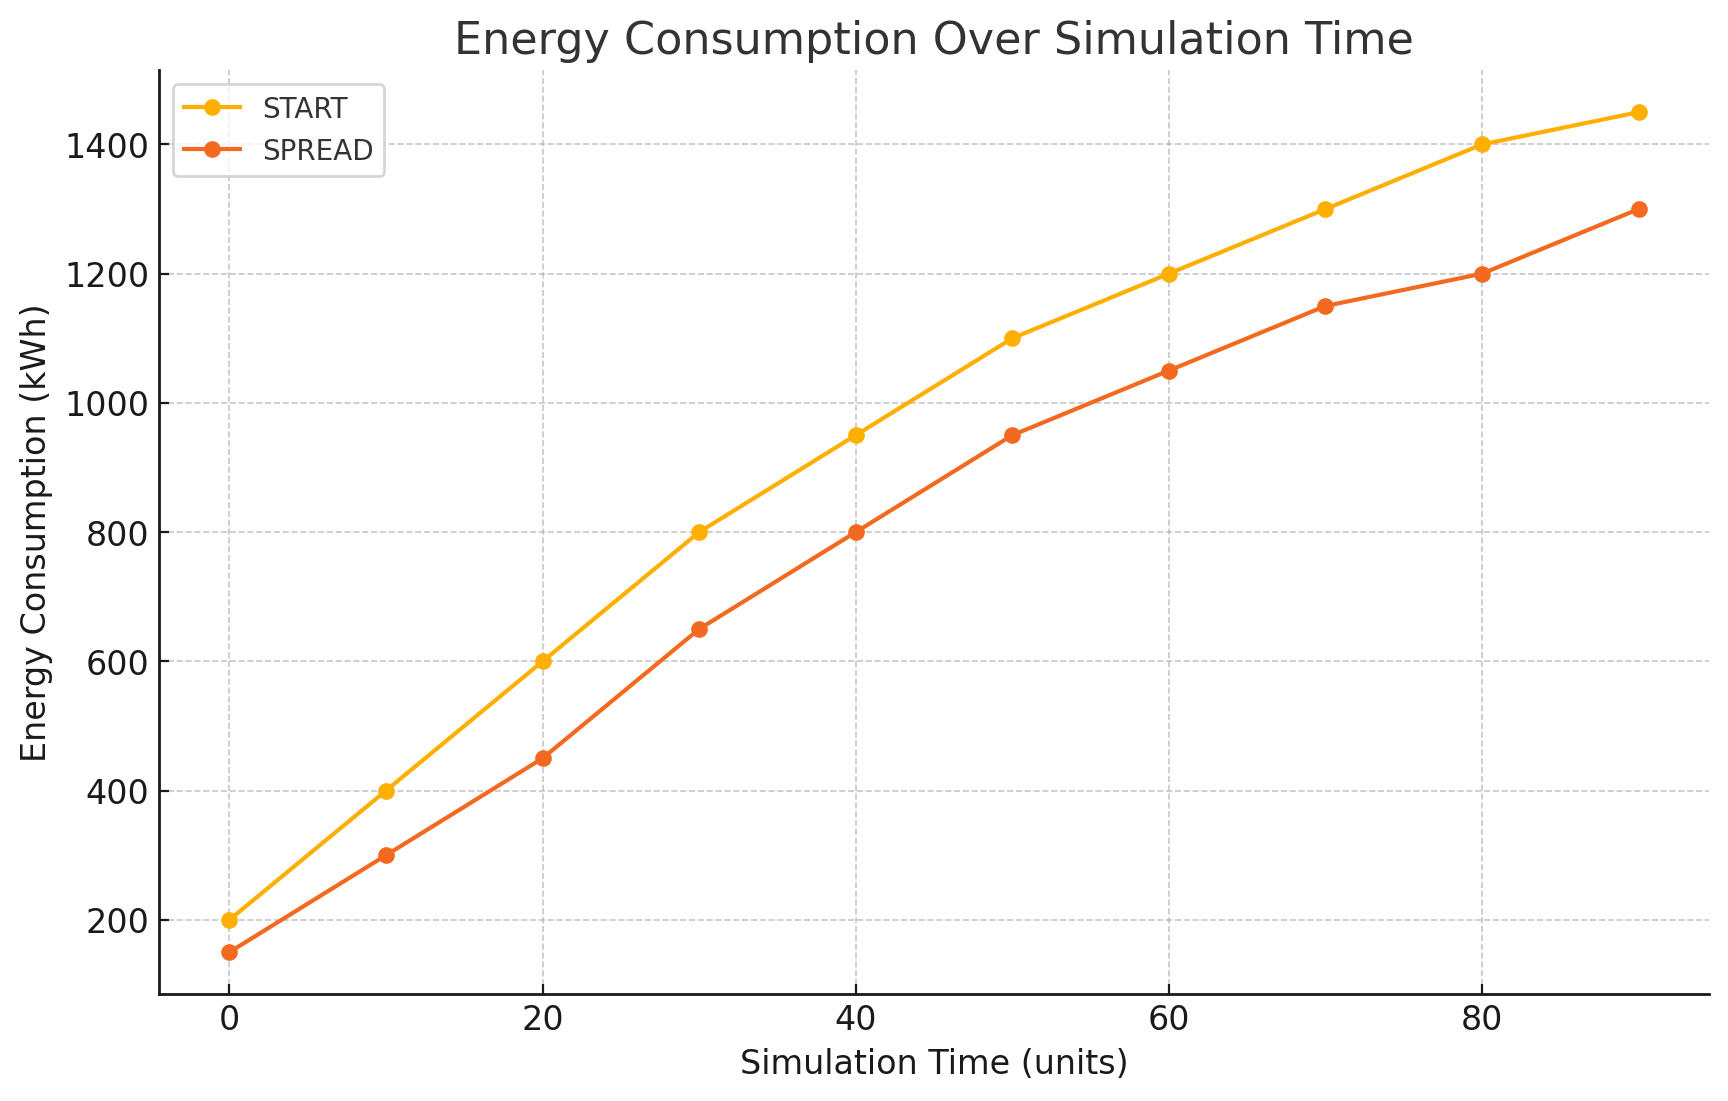
\includegraphics[width=0.8\textwidth]{Crest/Images/energy_consumption.png}
    \caption{Energy Consumption Over Simulation Time}
    \label{fig:energy_consumption}
\end{figure}

\begin{table}[h!]
\centering
\begin{tabular}{|c|c|c|}
\hline
\textbf{Simulation Step(\%)} & \textbf{START Mode} & \textbf{SPREAD Mode} \\ \hline
0  & 200  & 150  \\ 
10 & 400  & 300  \\ 
20 & 600  & 450  \\ 
30 & 800  & 650  \\ 
40 & 950  & 800  \\ 
50 & 1100 & 950  \\ 
60 & 1200 & 1050 \\ 
70 & 1300 & 1150 \\ 
80 & 1400 & 1200 \\ 
90 & 1450 & 1300 \\ \hline
\end{tabular}
\caption{Energy Consumption Over Simulation Time for START vs. SPREAD Modes}
\label{tab:energy_consumption}
\end{table}

% \paragraph{Idle Time:}
Before discussing the results, it is important to explain why the idle time shown in Figure~\ref{fig:idle_time_img} and Table~\ref{tab:idle_time_tab} gets smaller as the simulation goes on.  
In this simulation, every AEV is given an initial resting (idle) movement while it waits for a trip. As new TPs arrive and are assigned to vehicles, these idle periods are replaced by active tasks like picking up and dropping off passengers. Because of this, the total idle time across all vehicles reduces over time, instead of adding up.  
This behaviour comes directly from the way the reactive ride-sharing algorithm works: vehicles adjust their schedules as soon as a suitable trip becomes available, which helps to reduce the amount of time they are left idle.

As seen in Figure~\ref{fig:idle_time_img} and Table~\ref{tab:idle_time_tab}, the START mode cuts down idle time faster because all vehicles are available right from the beginning. In the SPREAD mode, idle time starts higher because vehicles are introduced gradually, but even here, idle time steadily falls as more vehicles are put into service.

\begin{figure}[h!]
    \centering
    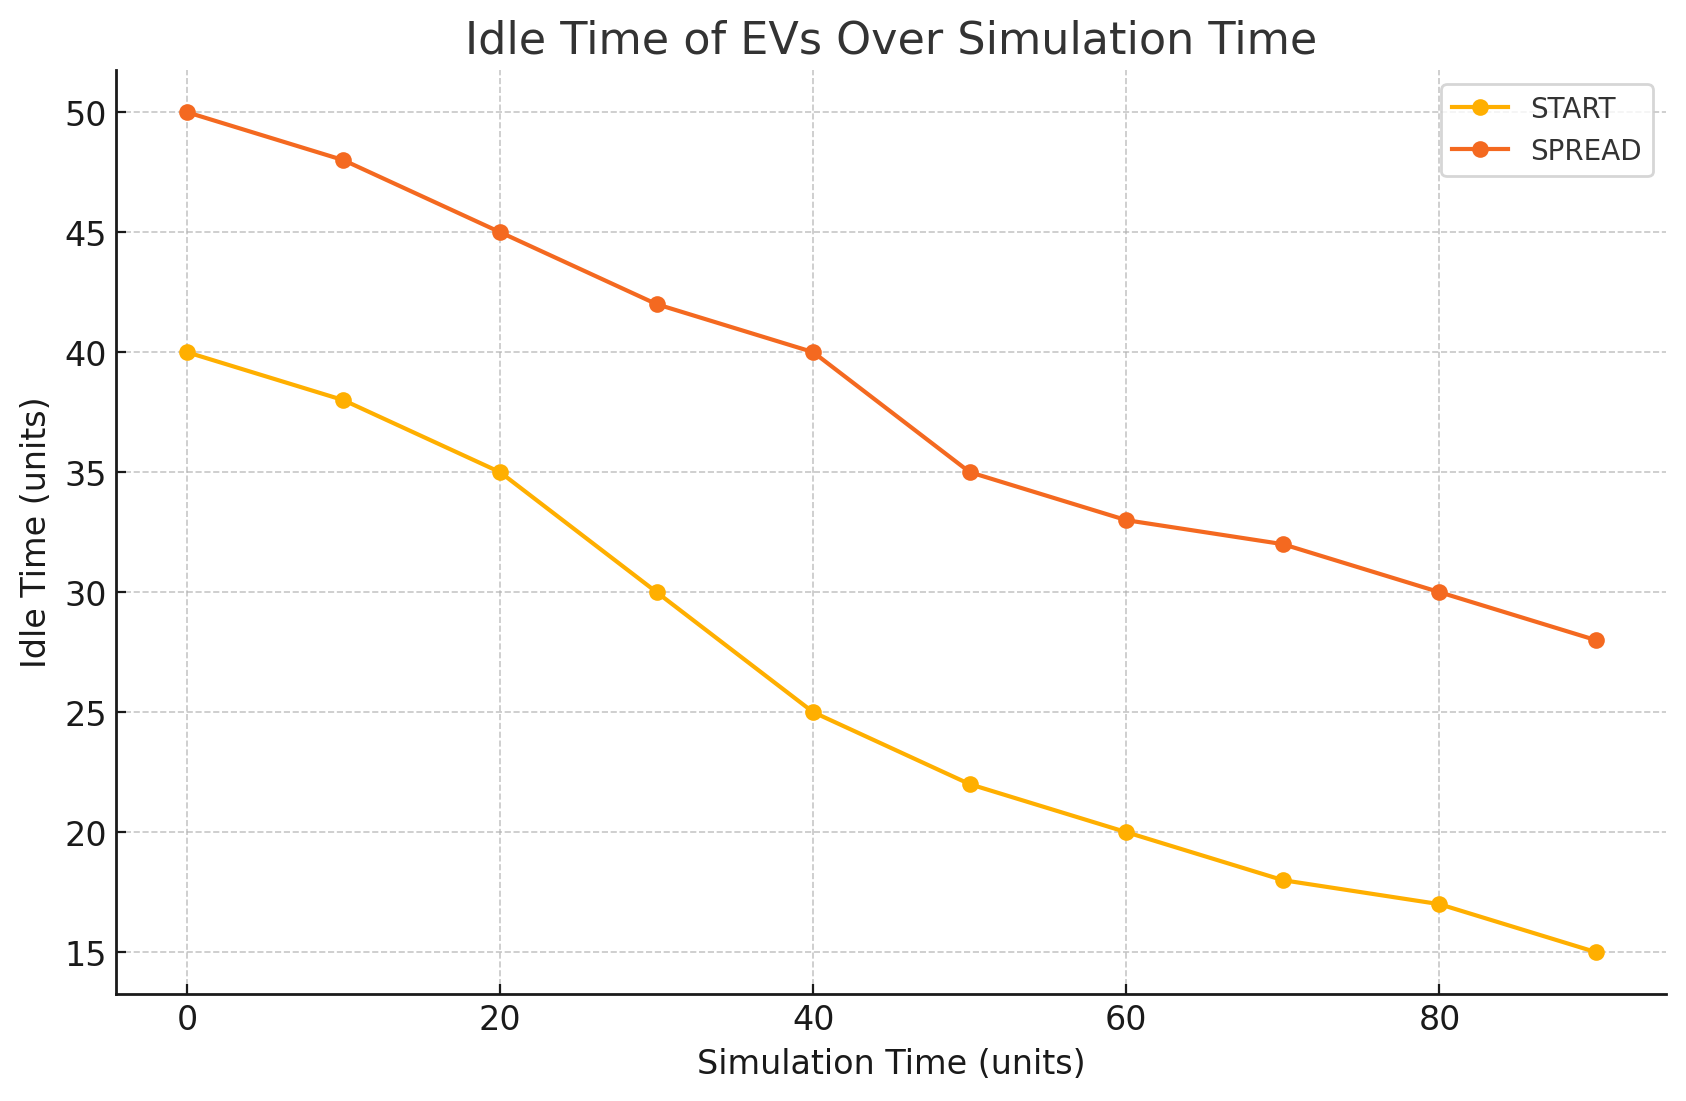
\includegraphics[width=0.8\textwidth]{Crest/Images/idle_time.png}
    \caption{Idle Time of AEVs Over Simulation Time (\%)}
    \label{fig:idle_time_img}
\end{figure}

\begin{table}[h!]
\centering
\begin{tabular}{|c|c|c|}
\hline
\textbf{Simulation Step (\%)} & \textbf{START Mode} & \textbf{SPREAD Mode} \\ \hline
0  & 40  & 50  \\
10 & 38  & 48  \\ 
20 & 35  & 45  \\ 
30 & 30  & 42  \\ 
40 & 25  & 40  \\ 
50 & 22  & 35  \\ 
60 & 20  & 33  \\ 
70 & 18  & 32  \\ 
80 & 17  & 30  \\ 
90 & 15  & 28  \\ \hline
\end{tabular}
\caption{Idle Time of AEVs Over Simulation Time for START vs. SPREAD Modes}
\label{tab:idle_time_tab}
\end{table}


% \subsubsection{Discussion}
The results show that the dispatch mechanism used has a substantial impact on the overall performance of the service. The START option is preferable in scenarios with strong demand early in the simulation. However, the SPREAD mode is more realistic in terms of RES generation, and more applicable in scenarios where resource conservation is crucial.

\subsection{Analysis - SEC Configurations on System Performance}
\label{sec:sec_configurations}

This experiment analyses the performance of the ride-sharing service across several SEC settings. A study of the number and distribution of SECs in various city layouts is done, with an emphasis on TPs served and energy consumption. The ideal configuration is discussed by experimenting with centralised, decentralised, and uneven SEC distributions.

\subsubsection{Experimental Parameters}
Three main SEC configurations are tested:
\begin{itemize}
    \item \textbf{Scenario 1 - Centralised SEC (1 SEC):} One SEC is placed at the centre of the city grid and owns all AEVs. This setup represents a centralised energy system, where all AEVs must return to a single point to recharge.

    \item \textbf{Scenario 2 - Uniformly Decentralised SECs (4 and 16 SECs):} In this scenario, two different configurations are tested. First, four SECs are evenly distributed across the city grid; then, sixteen SECs are also evenly distributed. Both configurations aim to reduce the travel distances of the AEVs and maintain a balanced energy supply across the area. The goal is to understand how increasing the number of uniformly distributed SECs affects system performance.

    \item \textbf{Scenario 3 - Non-uniform SEC Distribution:} This setup has four SECs grouped in one corner of the city grid, as shown in Figure~\ref{fig:non_uniform_sec}. 
\end{itemize}
\begin{figure}[h!]
    \centering
    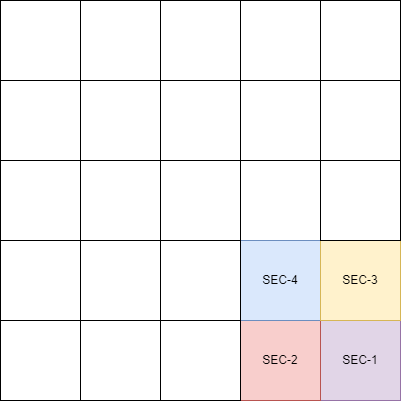
\includegraphics[width=0.5\textwidth, height=0.3\textheight]{Crest/Images/chapter_3_1_non_uniform_sec.png}
    \caption{Non-uniform SEC Distribution}
    \label{fig:non_uniform_sec}
\end{figure}

For each configuration, we test three different energy generation rates at SECs:
\begin{itemize}
    \item \textbf{Low Energy Generation:} Limited energy production, representing energy-scarce environments, 0.5 Energy factor (cf. Section 3.3.1).
    \item \textbf{Medium Energy Generation:} Balanced energy availability across SEC, 1.0 Energy Factor.
    \item \textbf{High Energy Generation:} Abundant energy production, allowing for rapid AEV launch and continuous operation, 2.0 Energy Factor.
\end{itemize}

Tables \ref{tab:trip_satisfaction_sec_refined} and \ref{tab:energy_efficiency_sec_refined} summarise the results of the experiments, comparing different SEC setups and energy generation rates.

Table \ref{tab:trip_satisfaction_sec_refined} and Figures \ref{fig:trip_satisfaction_rate},  \ref{fig:idle_time} show that the completely decentralised SEC configuration (16 SECs, uniformly distributed) has the highest trip satisfaction rate due to the localised position of the SECs, which decreases AEV transit time. The non-uniform distribution of SECs performs the worst, particularly at low energy generation rates, due to unequal vehicle availability.

Table \ref{tab:energy_efficiency_sec_refined} and Figure \ref{fig:energy_utilization} highlight that the centralised architecture (1 SEC) has higher energy efficiency during high energy generation rates (being able to release a good amount of AEVs over time, all of them initially located within reachable distance for any upcoming TP). However, this comes at the cost of having average longer routes for the AEVs. Decentralised arrangements are more suited to TPs due to reduced travel distances.

Table \ref{tab:energy_efficiency_sec_refined} and Figure \ref{fig:average_travel_distance} show that AEVs in the centralised SEC system travel significantly further than those in decentralised arrangements. Non-uniform SEC design result in varying trip distances.

\begin{table}[h!]
\centering
\resizebox{\textwidth}{!}{%
\begin{tabular}{|c|c|c|c|}
\hline
\textbf{SEC Configuration} & \textbf{Trip Satisfaction (\%)} & \textbf{Energy Level} & \textbf{Idle Time} \\ \hline
1 SEC (Centralised)         & 62.3  & Low    & 35 \\
1 SEC (Centralised)         & 70.0  & Medium & 30 \\
1 SEC (Centralised)         & 75.6  & High   & 28 \\
4 SECs (Uniform)            & 68.2  & Low    & 25 \\
4 SECs (Uniform)            & 80.1  & Medium & 22 \\
4 SECs (Uniform)            & 84.5  & High   & 18 \\
16 SECs (Decentralised)     & 78.0  & Low    & 15 \\
16 SECs (Decentralised)     & 85.7  & Medium & 18 \\
16 SECs (Decentralised)     & 89.69 & High   & 12 \\
4 SECs (Non-uniform)        & 50.5  & Low    & 40 \\
4 SECs (Non-uniform)        & 60.0  & Medium & 35 \\
4 SECs (Non-uniform)        & 65.0  & High   & 30 \\ \hline
\end{tabular}%
}
\caption{Trip Satisfaction Rate and Idle Time Across SEC Configurations and Energy Generation Levels}
\label{tab:trip_satisfaction_sec_refined}
\end{table}


\begin{table}[h!]
\centering
\resizebox{\textwidth}{!}{%
\begin{tabular}{|c|c|c|c|}
\hline
\textbf{SEC Configuration} & \textbf{Energy Utilised} & \textbf{Energy Level} & \textbf{Average Travel Distance} \\ \hline
1 SEC (Centralised)         & 8.5   & Low    & 95 \\
1 SEC (Centralised)         & 8.0   & Medium & 85 \\
1 SEC (Centralised)         & 7.9   & High   & 80 \\
4 SECs (Uniform)            & 7.8   & Low    & 70 \\
4 SECs (Uniform)            & 7.2   & Medium & 60 \\
4 SECs (Uniform)            & 6.9   & High   & 55 \\
16 SECs (Decentralised)     & 6.8   & Low    & 50 \\
16 SECs (Decentralised)     & 7.0   & Medium & 45 \\
16 SECs (Decentralised)     & 6.5   & High   & 40 \\
4 SECs (Non-uniform)        & 9.1   & Low    & 110 \\
4 SECs (Non-uniform)        & 8.5   & Medium & 95 \\
4 SECs (Non-uniform)        & 8.0   & High   & 90 \\ \hline
\end{tabular}%
}
\caption{Energy Utilisation and Average Travel Distance Across SEC Configurations and Energy Levels}
\label{tab:energy_efficiency_sec_refined}
\end{table}


% \begin{table}[h!]
% \centering
% \begin{tabular}{|c|c|c|}
% \hline
% \textbf{SEC} & \textbf{Average Travel Distance } & \textbf{Energy } \\ \hline
% 1 SEC (Centralised)         & 95   & Low    \\ 
% 1 SEC (Centralised)         & 80   & High   \\ 
% 4 SECs (Uniform)            & 60   & Medium \\ 
% 4 SECs (Non-uniform)        & 110  & Low    \\ 
% 16 SECs (Decentralised)     & 40   & High   \\ 
% 16 SECs (Decentralised)     & 45   & Medium \\ \hline
% \end{tabular}
% \caption{Average Travel Distance Across SEC Configurations and Energy Generation Rates}
% \label{tab:travel_distance_sec_refined}
% \end{table}

\begin{figure}[h!]
    \centering
    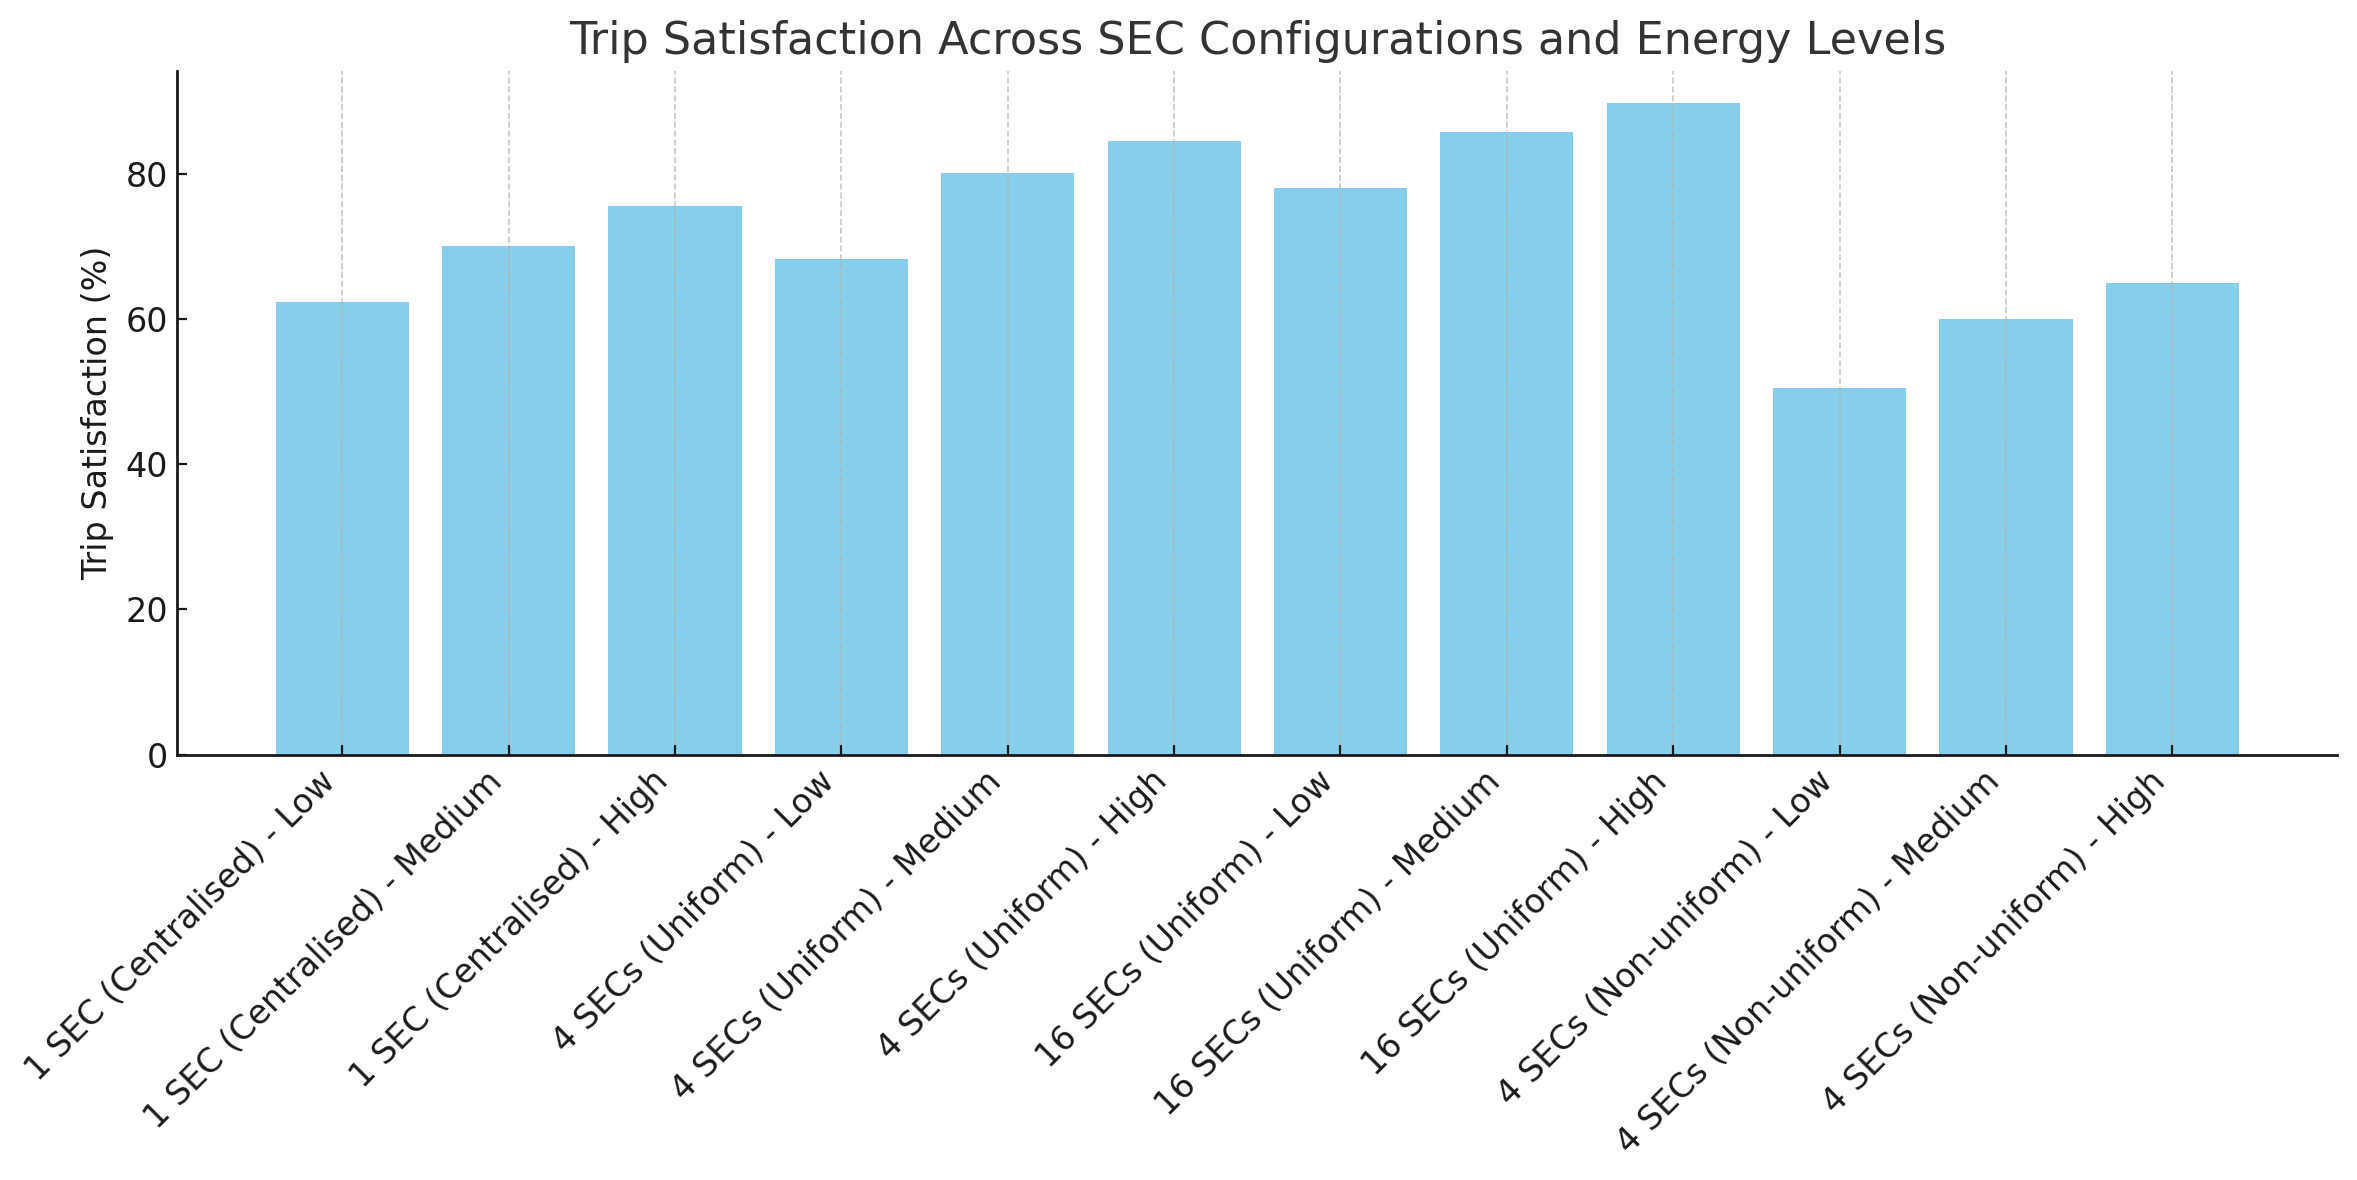
\includegraphics[width=0.8\textwidth]{Crest/Images/trip_satisfaction_rate.png}
    \caption{Trip Satisfaction Rate Over Simulation Time for Different SEC Configurations}
    \label{fig:trip_satisfaction_rate}
\end{figure}

\begin{figure}[h!]
    \centering
    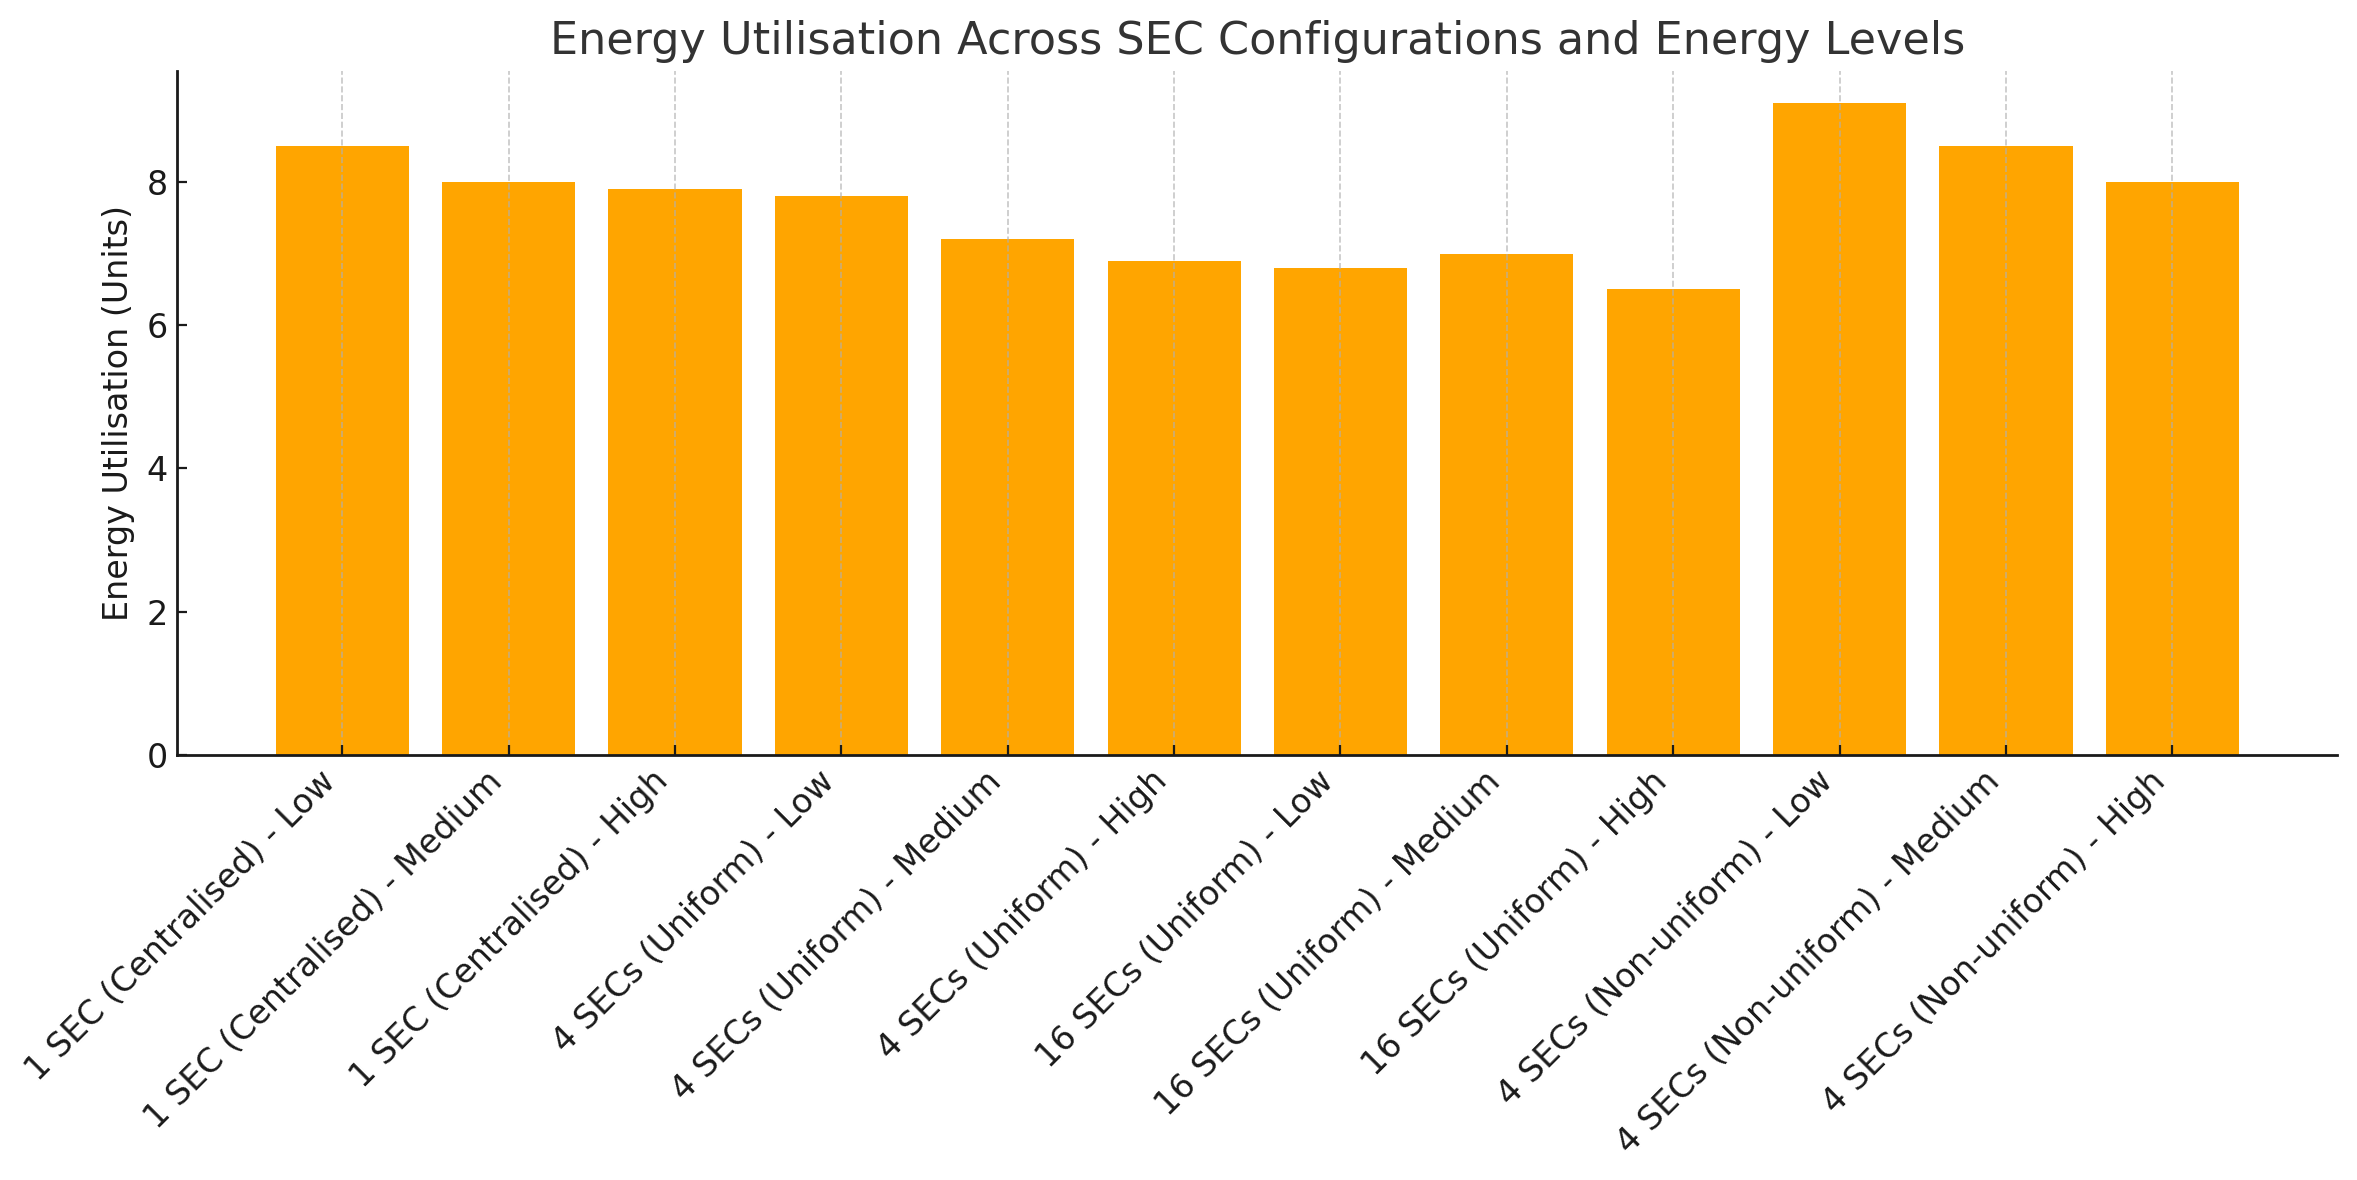
\includegraphics[width=0.8\textwidth]{Crest/Images/energy_utilisation.png}
    \caption{Energy Utilization Over Simulation Time for Different SEC Configurations}
    \label{fig:energy_utilization}
\end{figure}

\begin{figure}[h!]
    \centering
    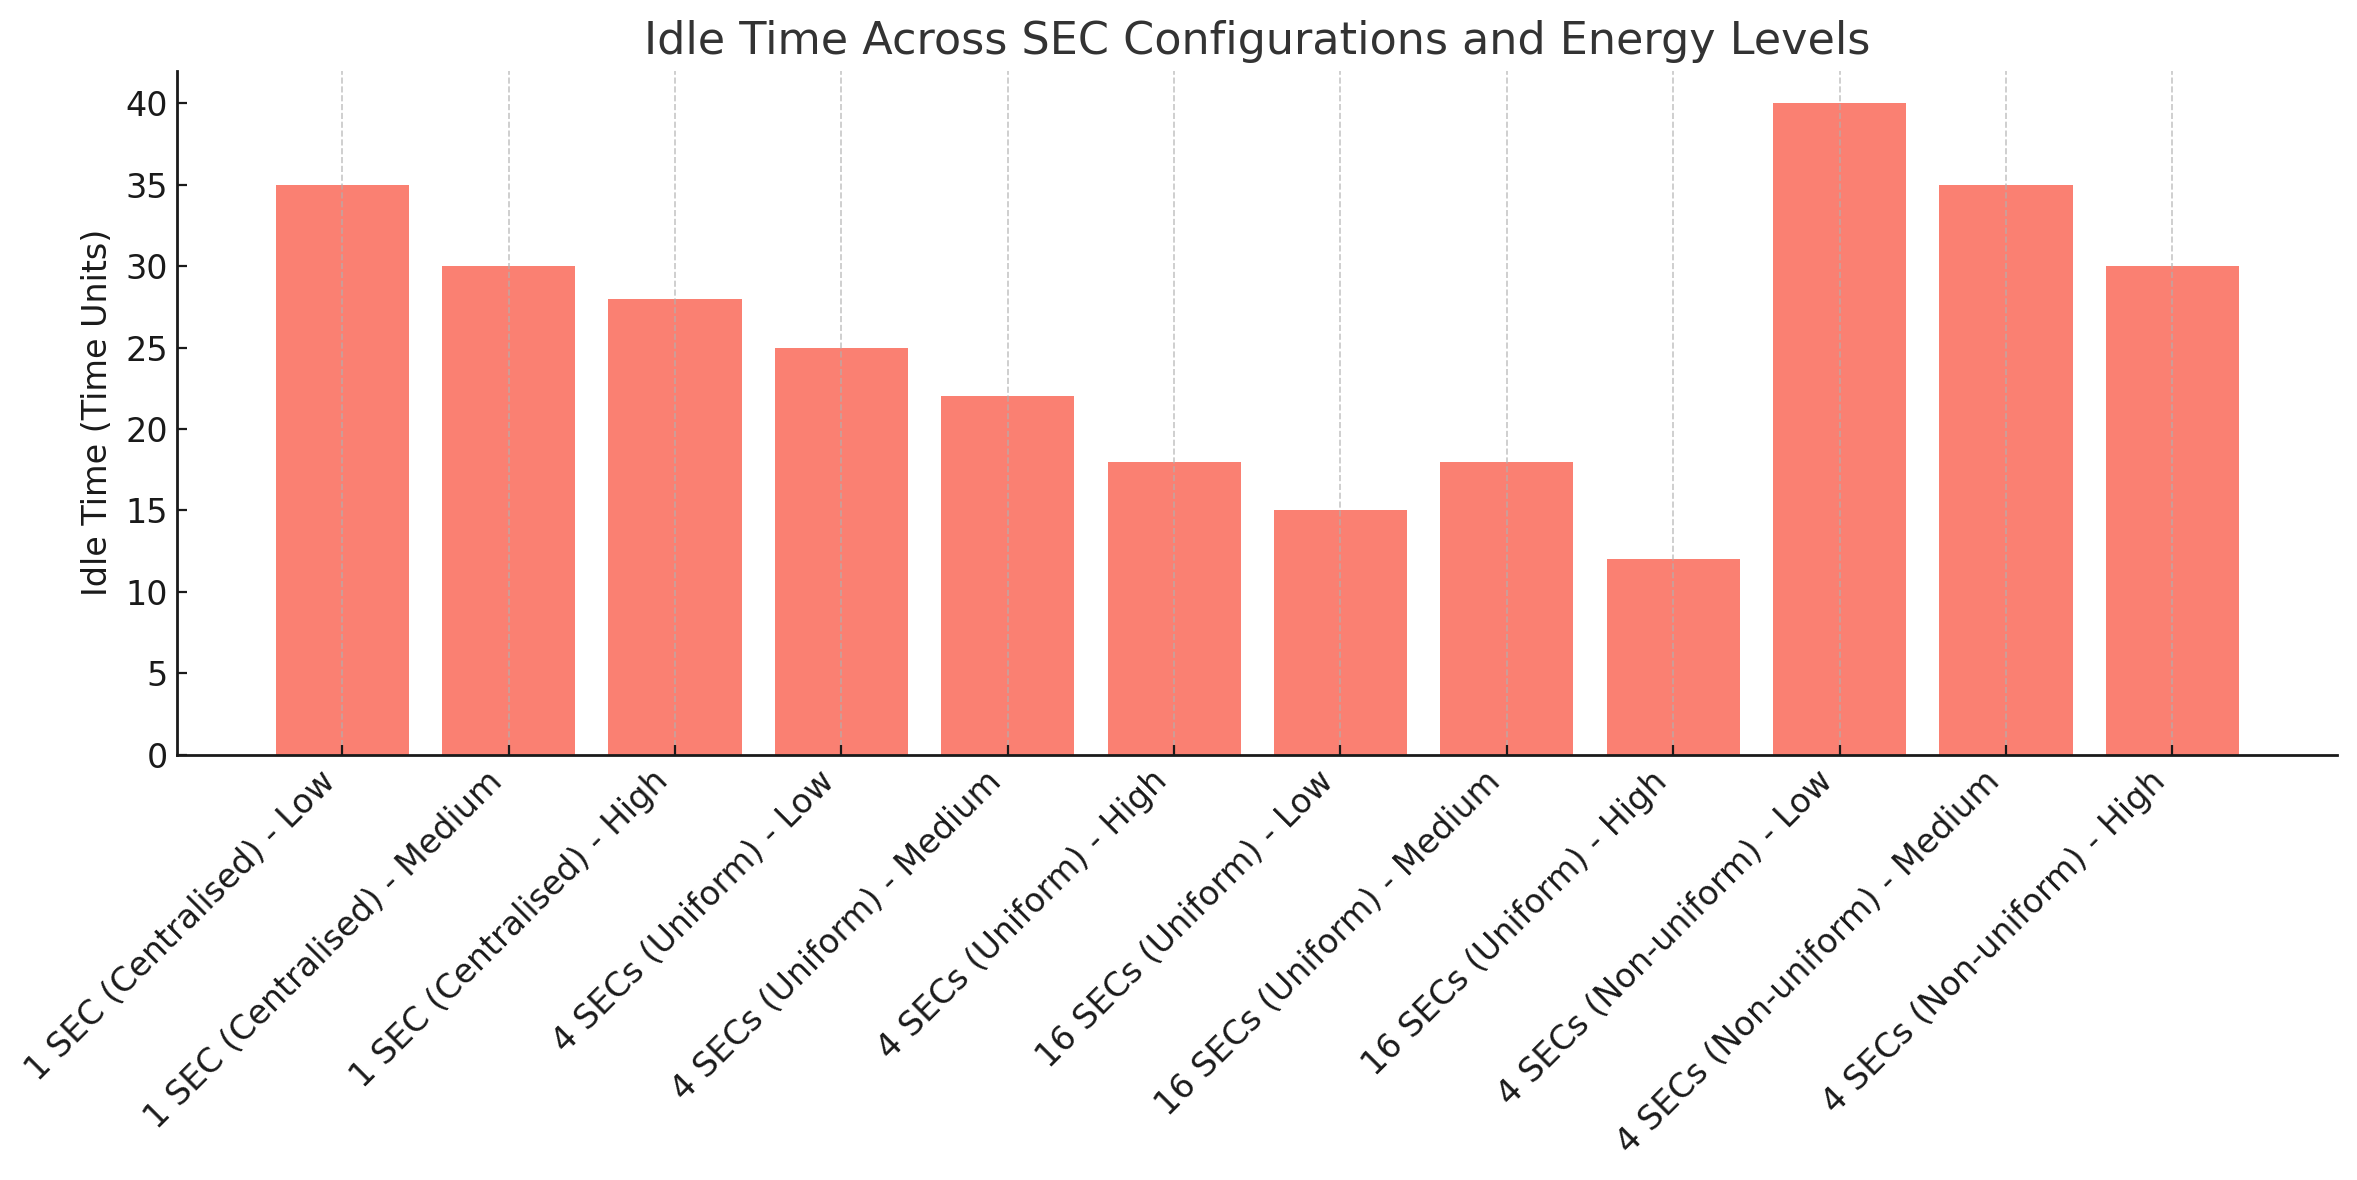
\includegraphics[width=0.8\textwidth]{Crest/Images/idle_time_sec_config.png}
    \caption{Idle Time Over Simulation Time for Different SEC Configurations}
    \label{fig:idle_time}
\end{figure}

\begin{figure}[h!]
    \centering
    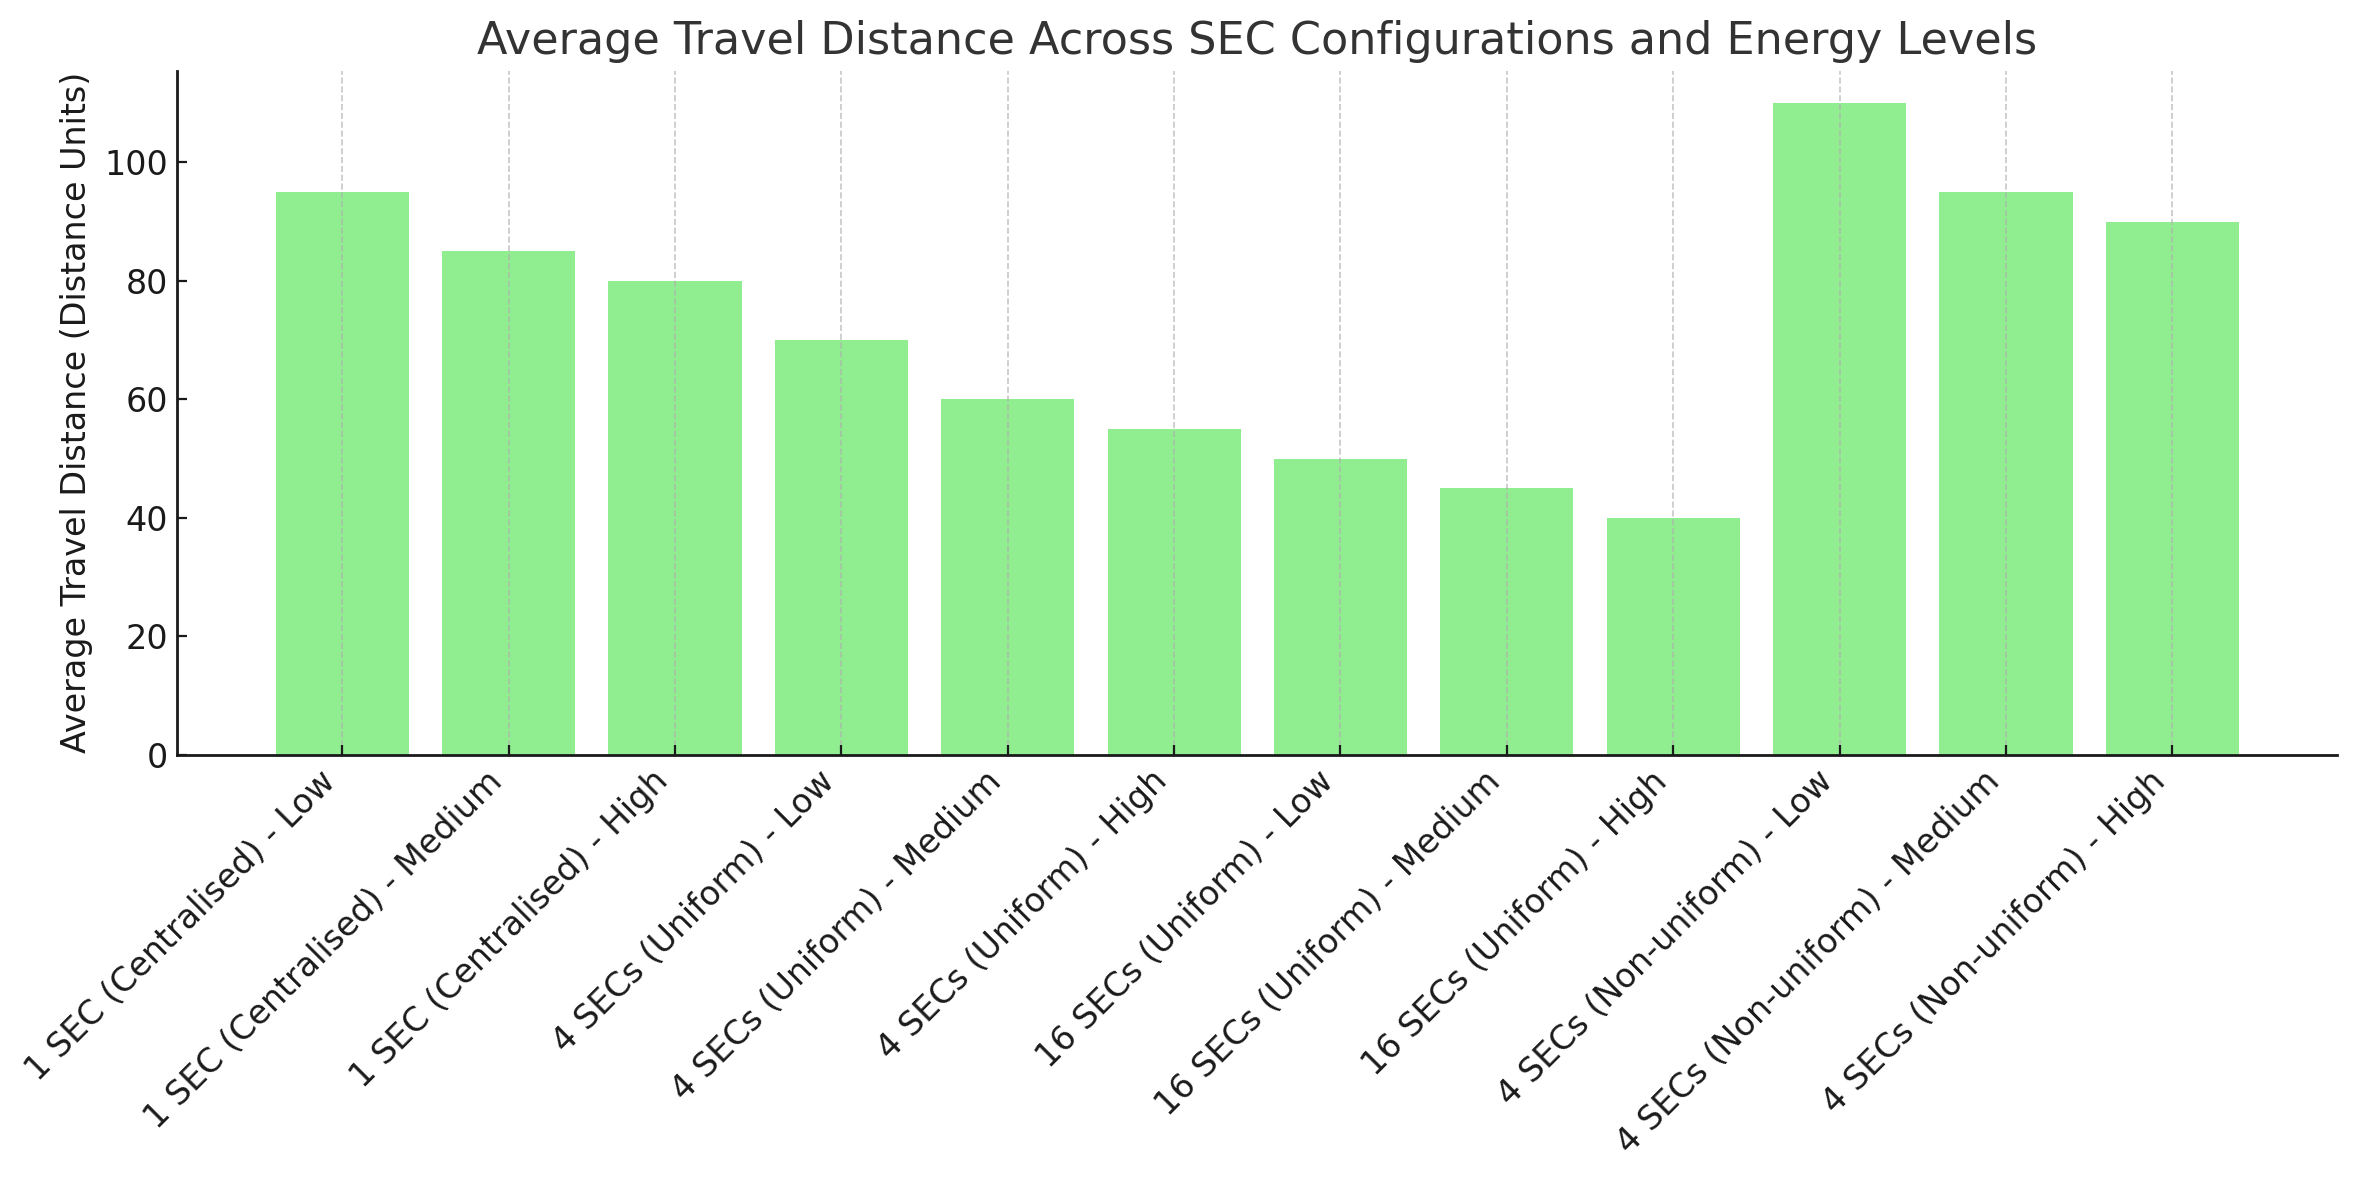
\includegraphics[width=0.8\textwidth]{Crest/Images/average_travel_distance.png}
    \caption{Average Travel Distance Over Simulation Time for Different SEC Configurations}
    \label{fig:average_travel_distance}
\end{figure}

The results show that decentralised SEC configurations, particularly those with uniform distribution, provide the highest overall performance in terms of TP served, energy consumption, and travel distances. In contrast, centralised SEC configurations, have longer travel times, making them less suitable for large city grids. Non-uniform SEC distributions produce the poorest performance due to uneven energy availability and inefficient vehicle placement.

The trade-off between centralised and decentralised systems is mostly determined by city size and energy generation capacity. For smaller cities with limited geographic spread, a centralised SEC arrangement may be adequate. However, in larger cities, decentralised designs, particularly those with uniform distribution, yield substantially superior results.


\section{Conclusions}
\label{sec:conclusion}
This chapter has presented the design, implementation, and evaluation of a carbon-neutral, community-based, reactive ride-sharing service for a smart city with 100\% AEVs operating solely over RES.  

The ride-sharing service has been formulated as a variant of the classical Dynamic Vehicle Routing Problem with Time Windows, with both dynamic resources and requests. The objective function has been set to maximise the overall number of TPs being served. The problem has been solved via a reactive-based simulation approach on top of a greedy-based decision-making process.  

An instance generator has been developed to create configurable scenarios to evaluate the proposed approach. It was used to extend existing benchmarks (Google HashCode) and public datasets (NYC taxis) to the problem formulation and testing the proposed algorithm under different settings. 

The ride-sharing service has proven to scale well,  with a quadratic algorithm complexity over its number of trips, allowing to solve an instance of about 1,000 trips in less than a second, and an instance of about 10,000 trips in less than two minutes.  Although favouring scalability over optimality, the service has proven to be able to solve up to ~90\% of the instances for some configurations of $d\_metropolis.in$, a complex instance from the Google HashCode.  
When applied to the real-world data-set of the NYC taxis and compared to an individual private transportation, the ride-sharing approach has been proven to offer a good trade-off between the amount of vehicles reduced (84\%) and its overhead in terms of distance traversed (21\%). The complete code can be accessed via GitHub \cite{smartgreenscode}. 
\chapter{Decentralised Vehicle Allocation for SEC-Based Ride-Sharing Services}
\label{chapter4}
Rapid urbanisation presents environmental and logistical difficulties \cite{Reference151}. This is particularly the case for rapidly growing cities, which are prone to dynamic urban environments and fluctuating travel demands \cite{Reference3020}. In such a context, the proliferation of SECs within the city presents a decentralised alternative to the traditional central management from the city authority, as each SEC can be independently in charge of managing its own AEV fleet and demands (TP requests from its neighbours).
Conventional ride-sharing systems typically fail to capture the complex dynamics of ride-sharing networks due to centralised optimisation methodologies \cite{Reference1,Reference2,Reference4,Reference6}. For the ride-sharing model presented in Chapter 3 to truly become applicable to large-scale cities, it must apply a decentralised approach enabling it to capture the complex dynamics among the different SECs placed in the city, their energy production and the ability of their AEV fleets to serve TPs. 

This chapter addresses such a problem by extending the ride-sharing model of Chapter 3, which focused solely on the formulation, solution approach and evaluation of the reactive ride-sharing service. A new model is designed, implemented and evaluated; its main goal is to capture the interrelation among the different SECs in the city as they compete for the allocation of the AEV fleet. The process is modelled as a decentralised negotiation process, deciding the number of AEVs allocated to each SEC. The new model works in tandem with the ride-sharing model of Chapter \ref{chapter3}; given its output (i.e., the partition of the AEV fleet among the SECs), each SEC then uses the ride-sharing model of Chapter 3 to serve the TPs of its own neighbouring SECs.

Specifically, the chapter includes the following contributions:

\begin{enumerate}
    \item The formulation of the vehicle allocation problem both as a centralised optimisation problem (using a
    Mixed-Integer Programming formulation) and as a decentralised one, using an iterative negotiation process
    among connected-SECs. On the latter, each SEC acts as an independent agent, and
    carries out a number of negotiations with any other SEC it is connected to over a simulated time horizon.
    In such negotiations, connected SECs decide the potential exchange of AEVs among them, based solely on their
    local information. The criticality of the vehicle allocation problem lies on its cooperation with its underlying ride-sharing problem to ensure adequate vehicle-to-passenger matching.
    Once assigned a fixed number of vehicles, the problem of each SEC operating its own ride-sharing service is solved using the ride-sharing model presented in Chapter \ref{chapter3}.
    
    \item The implementation of the vehicle allocation problem, using a novel Multi-Objective and Multi-Agent
    Reinforcement Learning (RL) algorithm, involving Deep Q-Learning with Graph Convolutional Networks. The algorithm
    equips SECs with the ability to learn from previous-negotiations,
    enabling them to improve their decision-making as the simulated time horizon goes by \cite{Reference103}.
    
    \item The evaluation of the solution approach for the problem tandem, measuring the performance of the solution approach under different SEC connectivity-levels
    and transport request distributions, when applied to the Google HashCode and NYC aligned datasets as described in Chapter 3. .
\end{enumerate}

The structure of the chapter is as follows:
\begin{itemize}
  \item \textbf{Section~\ref{sec:ccis_problem}} explains the vehicle‑allocation problem.
  \item \textbf{Section~\ref{ccis_reinforcement_learning_solution_approach}} describes how we solve it.
  \item \textbf{Section~\ref{sec:evaluation}} shows how we tested the solution.
  \item \textbf{Section~\ref{sec:conclusion}} sums up the results and outlines future work.
\end{itemize}

\section{Vehicle to SECs Allocation Problem}
\label{sec:ccis_problem}
This section presents the problem for the vehicle allocation in a SEC-based reactive ride-sharing service.
In it, a city contains a number of SECs, each of them responsible for operating the transport requests of its neighbours (linked SECs) via ride-sharing.
Given a fixed number of vehicles for the entire city, the problem is to decide the allocation of vehicles among the SECs,
and is formalised as a decentralised, iterative negotiation process among connected-SECs.

First, Subsection \ref{ccis_problem_overview} presents its problem overview.
Then, Subsection \ref{ccis_and_smartgreens_relationship} discusses its dependency on the ride-sharing problem,
Next, subsections \ref{ccis_centralised_formulation} and \ref{ccis_decentralised_formulation} present both a
hypothetical centralised formulation and its actual decentralised formulation, resp.
Finally, Subsection \ref{ccis_instance_example} presents an instance example.



%(and its cooperation with the ride-sharing problem, cf. Section \ref{sec:smartgreens_problem}).
%Subsection \ref{ccis_instance_example} presents an instance example.
%The two solution approaches to the problem, the Reinforcement Learning-based and the Mixed Integer Programming-based,
%are then discussed in sections \ref{ccis_reinforcement_learning_solution_approach} and \ref{ccis_heuristic_solution_approach}, resp.

\subsection{Problem Overview}
\label{ccis_problem_overview}

%The vehicle allocation problem extends the Single SEC Ride-sharing Problem to a new context, where
%a number of SECs in the city compete for the resources. It contains the following features:
The vehicle allocation problem contains the following features:
\begin{itemize}
%\item The grid dimensions of the city $c_r$,  $c_c$.
\item A number $numE$ of autonomous, homogeneous, electric vehicles (AEVs), representing the size of the vehicle fleet.
      Importantly, these AEVs belong now to the city, and are yet to be allocated.
\item A number $numC$ of SECs, spread across the city, and competing for the resources (AEVs).
      The SECs can be represented as a set C, where each SEC has its own specific id $c_i$
      and location in the city ($c_{ix}$,  $c_{iy}$).
\end{itemize}

The vehicle allocation outputs a set $VC\_Alloc$, representing a partition of the AEVs to the SECs of C.
%Each EV is to be assigned,
Each SEC $c_i$ is said to be assigned a specific number of AEVs $v_i$.
As all AEVs are homogeneous and, therefore, can be treated as counts instead of individual  units.
it is not necessary to individually identify any of these AEVs.
\[
VC\_Alloc = [ v_1, \ldots, v_{numC} ]
%\ \ \ \ \ \  \sum_{n=0}^{numC} c_{iv} = numE
\]

\subsection{From Vehicle Allocation to Ride-sharing}
\label{ccis_and_smartgreens_relationship}

Once a $VC\_Alloc$ is determined,
the problem is reduced to each SEC $c_i$ solving its own Single SEC Ride-sharing Problem,
operating the transport requests of its neighbours (its own set T of TPs associated to $c_i$) over the time horizon for the ride-sharing simulation $th$,
and outputting its own $Ci\_RS\_Alloc$, $Ci\_RS\_Sched$ and $Ci\_numtrip petitionsSat$ (c.f., chapter \ref{chapter3}).

Both $Ci\_RS\_Alloc$ and $Ci\_RS\_Sched$ involve the identification of individual AEVs, for their
allocation to TPs and routing. Therefore, the EV fleet can still be represented as a set E
(c.f., chapter \ref{chapter3}),
each vehicle with its own id $e_{id}$, battery capacity $e_{bc}$ and passenger capacity $e_{pc}$.
W.l.o.g., given the set E and $VC\_Alloc$, the mapping of E to C can be done by simply allocating the
first $c_{1v}$ AEVs of E to $c_1$, the next $c_{2v}$ to $c_2$, and so on.

Finally, given the ride-sharing solution of each SEC, the quality of the vehicle allocation
partition $VC\_Alloc$ is measured as the overall number of TPs serviced among all SECs $OverallNumtrip petitionsSat$
\[
OverallNumtrip petitionsSat = \sum_{n=1}^{numC} Ci\_numtrip petitionsSat
\]

\subsubsection{On Precomputing all Single SEC Ride-sharing Problems.}
The Vehicle Allocation Problem is a combinatorial optimisation problem.
Just in terms of $VC\_Alloc$, the amount of possible partitions of $numE$ AEVs among $numC$ SECs is:
$numE! / (numC! * (numE-numC)!)$
Therefore, even with a few SECs and vehicles, the number of possible partitions is intractable for brute force approaches.

On top of that, the tension of the problem lies in the relationship between a concrete partition
$VC\_Alloc_i = [ v_{1i}, \ldots, v_{numCi} ]$
and the underlying solution to the Single SEC ride-sharing Problem for each SEC $c_j$ (with the amount of vehicles $v_{ji}$
allocated by the partition $VC\_Alloc_i$ leading to $Ci\_numtrip petitionsSat$), in order to obtain the partition quality $OverallNumtrip petitionsSat$
associated to such $VC\_Alloc_i$.

From the perspective of a SEC $c_i$, its Single SEC Ride-sharing Problem is almost static,
as each time the only info that varies is the number of AEVs assigned to it $v_j$.
Therefore, it is possible for a SEC $c_i$ to maintain a look-up table $RS\_C_i\_Sols$ with the specific
ride-sharing problems being solved, so that they do not need to be recomputed again.
Furthermore, it is even possible to precompute the entire look-up table
for the entire range of AEVs $[0, \ldots, numE]$. Indeed, as all AEVs are homogeneous and available at the start of the
ride-sharing simulation, it might not even be needed to compute the entire range.
It might suffice with solve the problems increasingly in the number of AEVs;
as soon as the solution $numtrip petitionsSat$ for a number of AEVs $k+1$ is the very same as for the previous problem with $k$
vehicles, it is clear that adding an extra vehicle to the SEC has not allowed it to satisfy any new TP.
Therefore, there is no value in continuing to add more vehicles, and the solutions to the remaining range
$[k+1, \ldots, numE]$ can be straight away assigned to the same value $numtrip petitionsSat$ found for $k$ vehicles.
Last but not least, for a given problem with $numC$ SECs, the pre-computing of the look-up tables of
the different SECs can be done in parallel, as they are independent.

\subsection{Centralised Formulation}
\label{ccis_centralised_formulation}

If the EV partition $VC\_Alloc$ were considered to be computed by a centralised agent, with access to
all the information of all SECs, then the problem would become a centralised optimisation problem,
and could be formulated using a Mixed Integer Program (MIP) approach as the one below.

\textbf{Auxiliary Variables.} Let $Sols$ be an integer array concatenating the ride-sharing $RS\_Sols$ of each
SEC (such that the first $numE + 1$ elements of $Sols$ correspond to the $RS\_C_1\_Sols$,
the next $numE + 1$ elements to $RS\_C_2\_Sols$, and so on). Let also $NV$ be an integer array
concatenating the integer range $[0, \ldots, numE]$ as many times as SECs $numC$ there are.

\textbf{Decision Variables}. Let $X$ be a binary variable array of the same length as $Sols$ and $NV$.
                             Thus, each binary variable $x_{(i * numC) + j}$ denotes whether SEC $c_i$ is
                             allocated a number $j$ of AEVs (1) or not (0).
                             The range of variables in $X$ belonging to $c_i$ is $[i * (numE + 1), \ldots ((i+1) * (numE + 1))-1])$
\begin{enumerate}
\item[(1)] $\begin{aligned}[t]
    x_i \in [0, 1] \ \ \ \forall i\in [0, \ldots, numC \times (numE + 1)]
\end{aligned}$
\end{enumerate}

\textbf{Constraints}. Each SEC $c_i$ is required to be allocated to a unique number of vehicles. Therefore,
                      for each $c_i$, the sum of its range of variables in $X$ must be equal to 1.
\begin{enumerate}
\item[(2)] $\begin{aligned}[t]
    \sum_{n=i * (numE + 1)}^{((i+1) * (numE + 1))-1} x_n = 1 \ \ \ \forall i\in [0, \ldots, numC]
\end{aligned}$
\end{enumerate}
The amount of vehicles allocated to all SECs must be equal to $numE$.
\begin{enumerate}
\item[(3)] $\begin{aligned}[t]
    \sum_{n=0}^{numC \times (numE + 1)} x_n = numE
\end{aligned}$
\end{enumerate}

\textbf{Objective Function}. Given the above description, the $OverallNumtrip petitionsSat$ measuring the quality of a solution of
the Vehicle Allocation Problem is formalised as the cartesian product of $X$ and $Sols$. The goal
                            is to maximise such product.
\begin{enumerate}
\item[(4)] $\begin{aligned}[t]
    maximise \sum_{n=0}^{numC \times (numE + 1)} x_n \times sols_n
\end{aligned}$
\end{enumerate}

The application of this MIP formulation would lead to an optimal $VC\_Alloc$
(i.e., the one that maximises $OverallNumtrip petitionsSat$ w.r.t. the $RS\_Sols$ provided as input.)

\subsection{Decentralised Formulation}
\label{ccis_decentralised_formulation}

As opposed to the hypothetical centralised scenario presented above, the Vehicle Allocation Problem is
of decentralised nature, as each SEC $c_i$ acts as an independent agent, competing for resources
(its own share of AEVs in $VC\_Alloc$) based on the
partial information it has access to.

Interestingly, a pair of SECs ($c_i$, $c_j$) can
be connected (i.e., considered \textit{neighbours}), thus getting access to their respective information
(share in $VC\_Alloc$ and respective $RS\_Sols$) and
potentially exchanging AEVs if they agree to it.
This connectivity enables an undirected graph representation,
where each SEC $c_i$ is a node, and each pair of connected SECs ($c_i$, $c_j$) is an edge.
%Each SEC $c_i$ is aware of its own $RS\_C_i\_Sols$ and the one of any other $c_j$ it is connected to.
More importantly, the potential exchange of AEVs leads to
%an iterative negotiation process among connected SECs,
%making $VC\_Alloc$ to dynamically evolve over time.
%To model this
%a decentralised,
an iterative negotiation process among connected-SECs with the following features:
\begin{itemize}
\item \textbf{Time Simulation}. Similarly to the ride-sharing problem (dynamically handling TPs arriving over a
simulated time horizon $thr$), the vehicle allocation negotiation process handles potential AEVs exchanges over
a simulated time horizon $thv$.
\item \textbf{Negotiation Step}. The minimal, atomic step in the negotiation process is an EV exchange among
connected SECs.%, potentially arranging an exchange of AEVs between them.
This negotiation is said to happen at a given time unit $t$ of the time horizon $thr$.
\item \textbf{Local Decision-Making}.
The connected SECs negotiating in a step make the decision on whether to exchange AEVs or not based on their local information
(they know their current share in $VC\_Alloc$ and their respective $RS\_Sols$),
but lacking the global picture (they have no information on the shares in $VC\_Alloc$ and $RS\_Sols$ of the remaining
SECs not involved in the negotiation).
\item \textbf{Parallel Negotiations}.
Independent connected SECs can negotiate in parallel, at the same time $t$.
\item \textbf{Negotiation Cycle}.
An interval of time units $[ta, tb]$ represents a negotiation cycle if each SEC $c_i$ is involved in one
(and just one) negotiation step with each other SEC $c_j$ it is connected to.
\item \textbf{Negotiation Schedule}.
The length (number of time units) required by a negotiation cycle is decided by a negotiation schedule,
coordinating the negotiation steps among the connected SECs so that there are no overlaps among them (i.e.,
no SEC $c_i$ carries out two or more negotiation steps at the very same time unit).
\item \textbf{Vehicle Partition Evolution}.
As a result of the negotiations among connected SECs, the number of AEVs allocated to a SEC $c_i$
evolves over time. Therefore, the more general structures $NegVC\_Alloc$ and \\$NegOverallNumtrip petitionsSat$ are needed,
storing the resulting $VC\_Alloc$ and $OverallNumtrip petitionsSat$ of each time unit.
\item \textbf{Negotiation Start}.
The negotiation process $NegVC\_Alloc$ must start with a concrete initial $VC\_Alloc$ for time unit 0 (e.g., by evenly
splitting the AEVs among the SECs, with each $c_i$ receiving $numE / numC$ vehicles).
\item \textbf{Negotiation End}.
The negotiation process concludes when it either reaches the time horizon $thv$, or when it completes an entire
negotiation cycle with no single EV exchange among connected SECs.
\end{itemize}

\subsection{Instance Example}
\label{ccis_instance_example}

An instance \ref{fig:sched_AEV_1_TP_2} of the vehicle allocation problem presents a city of dimensions $n \times n$,
with 4 SECs $C \equiv [ C_1, C_2, C_3, C_4 ]$ placed in the top-left, top-right, bottom-left and bottom-right
quadrants, resp. Each SEC is placed half-way between the corner of its quadrant and the city centre location.
The SECs form a connected graph, with each pair of SECs ($c_i$, $c_{i+1}$) being connected.
Figure \ref{fig:myTinyCityFigure}(a) shows the city and its connected SECs. In this example, only negotiation steps
among two SECs ($c_i$, $c_j$) are considered. A negotiation
schedule of 2 time units is used, with SECs negotiating in the first (resp. second) step highlighted in blue (resp. red).
\begin{figure}[htbp]
    \centering
    \subfloat[SECs $C$]{\label{fig:tinyCity}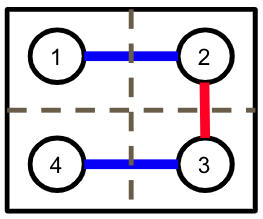
\includegraphics[width=0.25\textwidth]{Crest/Images/tinyGraph.png}}
    \qquad
    \subfloat[$RS\_Sols$]{\label{tab:solsTinyCity}
        \begin{tabular}[b]{c | c | c | c | c | c | c | c | c | c}
            \toprule
            VA & 0 & 1 & 2 & 3 & 4 & 5 & 6 & 7 & 8\\
            \midrule
            $C_1$ & 0 & 1 & 2 & 7 & 28 & 29 & 30 & 31 & 31\\
            $C_2$ & 0 & 22 & 26 & 27 & 28 & 29 & 30 & 30 & 30\\
            $C_3$ & 0 & 3 & 4 & 5 & 6 & 6 & 6 & 6 & 6\\
            $C_4$ & 0 & 1 & 27 & 29 & 30 & 31 & 32 & 32 & 32\\
            \bottomrule
        \end{tabular}
    }
    \qquad
    \subfloat[$NegVC\_Alloc$]{\label{tab:negVCTinyCity}
        \begin{tabular}[b]{c | c | c | c | c | c | c | c}
            \toprule
            Time & 0 & 1 & 2 & 3 & 4 & 5 & 6\\
            \midrule
            $C_1$ & 2 & 3 & 3 & 4 & 4 & 4 & 4\\
            $C_2$ & 2 & 1 & 2 & 1 & 2 & 2 & 2\\
            $C_3$ & 2 & 1 & 0 & 1 & 0 & 0 & 0\\
            $C_4$ & 2 & 3 & 3 & 2 & 2 & 2 & 2\\
            \hline
            $Exchange$ & - & 1-2 & 2-3 & 1-2 & 2-3 & - & -\\
                           &   & 3-4 &             & 3-4 &             &   &  \\
            \bottomrule
        \end{tabular}
    }
    \qquad
    \subfloat[$NegNumtrip petitionsSat$]{\label{tab:negNumtrip petitionsSatTinyCity}
        \begin{tabular}[b]{c | c | c | c | c | c | c | c}
            \toprule
            VA & 0 & 1 & 2 & 3 & 4 & 5 & 6\\
            \midrule
            $C_1$ & 2 & 7 & 7 & 28 & 28 & 28 & 28\\
            $C_2$ & 26 & 22 & 26 & 22 & 26 & 26 & 26\\
            $C_3$ & 4 & 3 & 0 & 3 & 0 & 0 & 0\\
            $C_4$ & 27 & 29 & 29 & 27 & 27 & 27 & 27\\
            \hline
            $OverallNumtrip petitionsSat$ & 59 & 61 & 62 & 80 & 81 & 81 & 81\\
            \bottomrule
        \end{tabular}
    }
    \caption{Vehicle Allocation Instance Example}
    \label{fig:myTinyCityFigure}
\end{figure}

The city has $numE \equiv 8$ AEVs to be allocated. A naive initial allocation evenly assigning 2 AEVs per SEC
is used (i.e., the initial $VC\_Alloc \equiv [2, 2, 2, 2]$). Figure \ref{fig:myTinyCityFigure}(c) shows how the number
of AEVs per SEC evolves over time as the
negotiation process progresses. For example, on time unit 1 a new column of the table is generated,
making $VC\_Alloc$ to evolve from $[2, 2, 2, 2]$ to $[3, 1, 1, 3]$.
The bottom row of the table highlights the negotiation steps leading to AEVs exchange on such time unit. (e.g., in time unit 1
both $(C_1, C_2)$ and $(C_3, C_4)$ agree to exchange AEVs among them). The amount of AEVs exchanged on each case can be
inferred by comparing consecutive rows of Figure \ref{fig:myTinyCityFigure}(c) (e.g., in time unit 0 $C_1$ and $C_2$
have 2 AEVs each, and in time unit 1 $C_1$ has 3 AEVs and $C_2$ has 1 EV, so they must have exchanged 1 EV).

A pair of SECs $c_i$ and $c_j$ decide on whether to exchange AEVs or not based on their local information;
they know both their current share in $VC\_Alloc$ (c.f. last column of Figure \ref{fig:myTinyCityFigure}(c))
and their respectives $RS\_Sols$ (c.f. Figure \ref{fig:myTinyCityFigure}(b)), which is a static table precomputed
in full before the negotiation process starts (c.f., Subsection \ref{ccis_and_smartgreens_relationship}).
However, the SECs $c_i$ and $c_j$ do not know the share
in $VC\_Alloc$ nor $RS\_Sols$ of any other SEC $c_z$ not involved in the negotiation.
For example, in time unit 1, when $C_1$ and $C_2$ start the negotiation with 2 AEVs each, they know they are currently
able to solve 2 and 26 TPs, resp. So, between them, 28 TPs. When they decide $C_1$ will borrow 1 AEVs from $C_2$,
they know this will lead to 7 and 22 TPs, resp. So, between them, 29 TPs, better than their current state. Similarly,
when $C_4$ borrows 1 AEVs from $C_3$, the two SECs pass from 31 TPs between them to 32 TPs.
Figure \ref{fig:myTinyCityFigure}(d)) shows how the number of TPs satisfied per SEC evolve over time, with its
last row measuring the $OverallNumtrip petitionsSat$, i.e., the quality of the current $VC\_Alloc$ (for example, in time unit 0
$OverallNumtrip petitionsSat$ is 59 TPs, but after the exchange of both ($C_1$, $C_2$) and ($C_3$, $C_4$) it reaches 61 TPs.

In the example the negotiation ends after 6 time units, as an entire negotiation cycle (steps 5 and 6) has happened
without a single EV exchange among connected SECs. During the negotiation process, $VC\_Alloc$ has evolved from
its initial $[2, 2, 2, 2]$ to $[4, 2, 0, 2]$ and the $OverallNumtrip petitionsSat$ from 59 TPs to 81 TPs.
The example confirms that a lightweight, pairwise strategy can converge rapidly to a
near‑optimal allocation, even with minimal initial information and only local decision‑making.

In this model, the SECs are assumed to behave as cooperative agents rather than strictly self-interested entities. Their negotiation decisions are guided by the collective goal of maximising the total number of TPs satisfied across the entire system. Although each SEC operates with local information—aware only of its own share in $VC\_Alloc$ and its precomputed $RS\_Sols$—the negotiation strategy is designed to promote exchanges that lead to global improvements.

For example, during a negotiation between $C_1$ and $C_2$ in time unit 1, both SECs assess whether reallocating an AEV results in a higher combined number of TPs satisfied. If this condition is met, the exchange proceeds, even if one SEC temporarily sacrifices resources. This cooperative approach reflects the underlying design of Smart Energy Communities, which aim to balance individual and collective benefits through resource sharing.

It is important to note that the model abstracts away from complex, self-interested behaviours or strategic deception, focusing instead on evaluating the performance of lightweight, decentralised, pairwise negotiations under cooperative assumptions. Future work could explore more adversarial or competitive negotiation dynamics.


\section{Reinforcement Learning-based Solution Approach}
\label{ccis_reinforcement_learning_solution_approach}

In this section, the chapter introduces a reinforcement learning-based solution as a decentralised approach to address the vehicle allocation problem \cite{Reference301} described in sections \ref{sec:ccis_problem}. 

\subsection{Deep Reinforcement Learning}
Deep Reinforcement Learning (DRL) trains agents to optimise cumulative rewards while making decisions \cite{Reference501}. Reinforcement learning and deep neural networks allow agents to learn complicated patterns and representations \cite{Reference501}.

\subsubsection{Q-Networks}
Q-networks are neural networks that approximate the Q-function, which estimates the expected cumulative reward an agent can obtain by taking a certain action from a given state and following a specific policy thereafter. The Q-network takes the current state as input and outputs Q-values for all possible actions, enabling the agent to make decisions that lead to higher rewards. The Q-value is calculated using the Bellman Equation \cite{Reference501}. 
\[
Q(s, a) = \sum_{s'} p(s' \mid s, a) \left[ r(s, a, s') + \gamma \max_{a'} Q(s', a') \right]
\]

Where:
\begin{align*}
Q(s, a) & : \text{Q-value for state-action pair }(s, a) \\
s & : \text{Current state} \\
a & : \text{Taken action in state } s \\
s' & : \text{Next state} \\
r(s, a, s') & : \text{Immediate reward obtained upon transitioning from state }  s\\ \text{ to state } s' \text{ with action } a \\
p(s' \mid s, a) & : \text{Transition probability to state } s' \text{ given action } a \text{ in state } s \\
\gamma & : \text{Discount factor that balances future rewards} \\
a' & : \text{Possible actions in state } s'
\end{align*}

% \subsubsection{Neural Networks}

% Neural networks are a class of machine learning models inspired by the structure and function of the human brain. They consist of interconnected nodes, called neurons, organised in layers. Each connection between neurons has associated weights that are learned during training. Neural networks can approximate complex functions and capture intricate relationships in data, making them suitable for tasks like function approximation, classification, and regression \cite{Reference502}.

\subsection{Problem Modeling}
In this formulation, each SEC acts as an independent agent that:

\begin{enumerate*}[label=(\roman*)]
    \item observes its local state (including available AEVs, pending TPs, and information from neighbouring SECs),
    \item selects an action (the fraction of AEVs to dispatch or retain),
    \item receives a reward balancing service quality and energy efficiency, and
    \item transitions to a new state, updating fleet distribution and trip queues.
\end{enumerate*}

The remainder of this subsection formally describes the Markov-game tuple \(M=(C, S, A, P, R, \gamma)\),where:

\begin{itemize}
    \item \(C\) is the set of agents, with each agent representing a SEC.
    \item \(S\) is the set of states, with each SEC maintaining its own state \(s_t^i\) at simulation step \(st\), incorporating the spatial distribution of available AEVs and TPs.
    \item \(A\) is the set of joint actions, allowing each agent to choose a fraction of available AEVs to dispatch to neighbouring SECs, represented as $a_t^i \in [0, 1]$. Each action $a_t^i \in A_i$ represents the fraction of available AEVs at SEC $c_i$ that will be dispatched to neighbouring SECs in the next simulation step $st+1$. For example, $a_t^i = 0.5$ means half of the available AEVs at SEC $c_i$ will be dispatched to neighboring SECs.
        \[ A_i = [0, 1] \]
    \item \(P\) represents the state transition probability which are deterministic. A $\epsilon$-greedy learning strategy, with a gradually decaying value of $\epsilon$ (exploration rate) is employed based on which an agent can choose to either take an action to explore the environment or an action that gains it the maximum reward based on its Q-network.
    \item \(R\) is the reward function that guides the decision making of the agents. It combines metrics such as petitions served and energy efficiency, as well as a shaping reward promoting efficient dispatching. It balances these factors through a weight parameter \(\alpha\)
        \begin{multline*}
            R_i(s_t, a_t^i) = \text{Petitions Served} - \\
            \alpha \cdot \text{Energy Usage of Dispatched AEVs}
            + R_{\text{shaping}}^i(s_t, a_t^i)
        \end{multline*}
        \begin{multline*}
                R_{\text{shaping}}^i(s_t, a_t^i) = -\alpha \cdot \text{Distance Covered by Dispatched AEVs} \\
                + \gamma \cdot \text{Petitions Served}
        \end{multline*}
    \item \(\gamma\) is the discount factor that determines the importance of future rewards.
\end{itemize}

\subsection{Instance Example}

For illustration purposes, a scenario involving three agents (SECs) denoted as \(A\), \(B\), and \(C\)is considered. The state of each agent at step \(st=0\) is represented by the number of available AEVs (\(EV_t^i\)) and the number of pending TPs (\(TP_t^i\)) in their respective service areas. The agents also select actions (\(a_t^i\)) by choosing a fraction of available AEVs to dispatch to neighbouring SECs. The reward function (\(R_i(s_t, a_t^i)\)) combines the number of petitions served, the energy usage of dispatched AEVs, and a shaping reward.

The following initial states and actions:

\begin{itemize}
    \item Agent \(A\): \(s_0^A = (8, 3)\) (8 available AEVs and 3 pending TPs)
    \item Agent \(B\): \(s_0^B = (5, 2)\) (5 available AEVs and 2 pending TPs)
    \item Agent \(C\): \(s_0^C = (7, 4)\) (7 available AEVs and 4 pending TPs)
\end{itemize}

The agents then choose actions for dispatching AEVs:

\begin{itemize}
    \item Agent \(A\): \(a_0^A = 0.6\) (60\% of available AEVs dispatched)
    \item Agent \(B\): \(a_0^B = 0.3\) (30\% of available AEVs dispatched)
    \item Agent \(C\): \(a_0^C = 0.4\) (40\% of available AEVs dispatched)
\end{itemize}

Assuming the following parameter values:
\begin{itemize}
    \item \(\alpha = 0.5\) (weight parameter for shaping reward)
    \item \(\gamma = 0.8\) (discount factor for shaping reward)
    \item Distance covered by each dispatched EV = 10 units
    \item Energy usage of each dispatched EV = 10 units
\end{itemize}

Based on these initial states, actions, and assumed parameter values, the shaping reward (\(R_{\text{shaping}}^i(s_t, a_t^i)\)) for each agent can be calculated:

\begin{itemize}
    \item Agent \(A\): 
    \[
    R_{\text{shaping}}^A(s_0^A, a_0^A) = -0.5 \cdot 10 + 0.8 \cdot 3 = -5 + 2.4 = -2.6
    \]
    \item Agent \(B\): 
    \[
    R_{\text{shaping}}^B(s_0^B, a_0^B) = -0.5 \cdot 10 + 0.8 \cdot 0 = -5 + 0 = -5
    \]
    \item Agent \(C\): 
    \[
    R_{\text{shaping}}^C(s_0^C, a_0^C) = -0.5 \cdot 10 + 0.8 \cdot 4 = -5 + 3.2 = -1.8
    \]
\end{itemize}

Finally, the total reward (\(R_i(s_t, a_t^i)\)) for each agent can be calculated by incorporating the shaping reward:

\begin{itemize}
    \item Agent \(A\): 
    \[
    R_A(s_0^A, a_0^A) = \text{Petitions Served} - 0.5 \cdot 10 - 2.6
    \]
    \item Agent \(B\): 
    \[
    R_B(s_0^B, a_0^B) = \text{Petitions Served} - 0.5 \cdot 3 - (-5) = \text{Petitions Served} - 0.5 \cdot 3 + 5
    \]
    \item Agent \(C\): 
    \[
    R_C(s_0^C, a_0^C) = \text{Petitions Served} - 0.5 \cdot 4 - (-1.8) = \text{Petitions Served} - 0.5 \cdot 4 + 1.8
    \]
\end{itemize}

The scenario example mentioned above represents a single step. In a reinforcement learning context, a complete sequence of actions, states, rewards, and transitions forms an episode. Each episode corresponds to a cycle of decision-making, action execution, state transitions, and rewards that occurs over a series of steps. The reinforcement learning algorithm learns from these episodes to develop an optimal policy that maximises cumulative rewards over time, adapting to the changing environment and interactions between agents.

\subsection{Decentralised DQN with Experience Sharing and GCN}
\label{sec:decentralised_dqn_gcn}

This subsection presents an enhanced decentralised DQN framework integrated with GCN \cite{Reference106}. The goal of this integration is to enable effective experience sharing and improve decision-making among SECs during the vehicle-allocation negotiation process.

% Learning Process Equations
Each SEC operates independently in its environment and interacts with the grid world. It selects an action based on an $\epsilon$-greedy policy using its own Q-network and exploration rate ($\epsilon$).

The SEC executes the action, receives a reward, and transitions to the next state. The experience tuple (state, action, reward, next\_state) is stored in the replay memory of the SEC.

The replay memory follows a First-In-First-Out (FIFO) mechanism, where old experiences are replaced with new experiences when the memory capacity is reached. The replay memory is used during the training process to sample random mini-batches of experiences. These mini-batches are then used to update the Q-network, allowing the agent to learn from a diverse set of experiences and improve its decision-making capabilities.

Mathematically, the replay memory can be defined as:
\[ D = \{(s, a, r, s')_1, (s, a, r, s')_2, \ldots, (s, a, r, s')_N\} \]

where $(s, a, r, s')_i$ represents the $i$-th experience stored in the memory. 

% Experience Sharing Equations and Diagram
Periodically, each SEC samples a random mini-batch of experiences from its replay memory $D$.

Now, to enhance the learning process and enable experience sharing between SECs, GCNs are introduced. A GCN performs iterative message passing between neighboring nodes (SECs) in the graph, enabling each SEC to incorporate information from its neighbors.

In the context of the grid world with SECs, each SEC corresponds to a node in the graph, and there are edges between spatially neighboring SECs. The features of each SEC (e.g., number of available AEVs, trips satisfied, energy consumed) form the node attributes.

The GCN aggregates information from neighboring SECs and updates the features and experience of the current community. This process enables the SEC to learn from the experiences of other SECs through the shared graph information.

Consider a simplified scenario with three SECs: communities A, B and C. These SECs are spatially connected in a grid-based system. Each SEC aims to optimise its energy allocation strategy to maximise the number of TPs served while minimising energy consumption.

Suppose we have the following features for each SEC:

\begin{itemize}
    \item SEC A: $\text{Num\_AEVs} = 50$, $\text{Num\_TPs} = 100$, $\text{Energy} = 700$
    \item SEC B: $\text{Num\_AEVs} = 30$, $\text{Num\_TPs} = 90$, $\text{Energy} = 600$
    \item SEC C: $\text{Num\_AEVs} = 40$, $\text{Num\_TPs} = 80$, $\text{Energy} = 400$
\end{itemize}

Initially, each SEC operates independently, using its own experience and Q-network to make decisions.

Imagine that SEC A wants to update its Q-values based on its experience and the experiences of its neighboring SECs (B and C). Through the GCN-based experience sharing mechanism, SEC A aggregates information from SECs B and C and updates its own features.

For example, suppose SEC A uses a simple message aggregation process where it takes an average of the features of its neighbors:

% \[
% \begin{aligned}
%     \text{New\_Num\_AEVs} &= \frac{\text{Num\_AEVs\_A} + \text{Num\_AEVs\_B} + \text{Num\_AEVs\_C}}{3} \\
%     % \text{New\_Num\_trip petitions} &= \frac{\text{Num\_trip petitions\_A} + \text{Num\_trip petitions\_B} + \text{Num\_trip petitions\_C}}{3} \\
%     % \text{New\_Energy} &= \frac{\text{Energy\_A} + \text{Energy\_B} + \text{Energy\_C}}{3}
% \end{aligned}
% \]
\[
\text{New\_Num\_AEVs} = \frac{1}{3} \sum_{i=A}^{C} \text{Num\_AEVs\_i}
\]


This averaging process integrates information from neighboring SECs. After the aggregation, the new features for SEC A become:
\begin{itemize}
    \item $\text{New\_Num\_AEVs} = 40$
    \item $\text{New\_Num\_TPs} = 90$
    \item $\text{New\_Energy} = 566.67$
\end{itemize}

Now, SEC A can use these updated features in its Q-network to make more informed decisions. By considering information from neighboring SECs, SEC A can learn from their experiences, understand the overall energy allocation dynamics in the network, and adjust its EV allocation strategy. 

\subsection{Algorithm Overview}
This subsection describes of the proposed Decentralised DQN-GCN algorithm through pseudocode. Specifically, Algorithm 2 illustrates how messages (or experiences) are shared among neighbouring SECs using a GCN. Each SEC (node \( v_i \) in graph \( \mathcal{G} \)) aggregates relevant information from its neighbours to enhance its own learning and decision-making process. The function \(\text{Neighbors}(v_i)\) identifies neighbouring SECs directly connected to \( v_i \), enabling each community to learn not only from its own experiences but also from the experiences of its peers.


% Algorithm \ref{algo:gcn} presents the pseudocode for message passing. It assumes that $\text{Neighbors}(v_i)$ is a function that returns the set of neighboring nodes of $v_i$ in the graph $\mathcal{G}$. 

The learning process involves a series of steps that enable each SEC to operate effectively within the ride-sharing environment, making informed decisions through the integration of GCNs for experience sharing and learning. A three-layer GCN was adopted to capture both immediate and second-order neighbourhood information without introducing excessive depth that could cause over-smoothing or vanishing gradients. The number of neurons per layer is set to match the number of SECs in the system, ensuring a direct, interpretable mapping between graph nodes and learned representations. The ReLU activation function and a learning rate of $\alpha = 0.001$ were chosen following preliminary tuning experiments, balancing training stability and learning speed.

These parameter choices reflect a trade-off between model complexity and the practical requirements of operating on dynamic, city-scale graphs representing SEC interactions.
\begin{algorithm}[hb]
\caption{Message Passing in GCN for Decentralised Deep Q-Learning with GCN Experience Sharing}
\small % Adjust font size
\SetAlgoLined
\SetKwInOut{Input}{Input}
\SetKwInOut{Output}{Output}

\Input{Graph $\mathcal{G}$ for each SEC, GCN architecture parameters, GCN hyperparameters}
\Output{Updated graph representation for each SEC}

\ForEach{SEC in SECs}{
    \textbf{Initialize} node embeddings $\mathbf{H}$ for each node in $\mathcal{G}$ with random values\;
}

\ForEach{layer in GCN layers}{
    \ForEach{SEC in SECs}{
        \textbf{Initialize} message aggregator $\mathbf{M}_v$ for each node $v$ in $\mathcal{G}$ with zeros\;
        
        \ForEach{node $u$ with an edge to $v$}{
            \textbf{Aggregate} messages from neighbors: $\mathbf{M}_v \pluseq \text{Aggregator}(\mathbf{H}_u)$\;
        }
        
        \textbf{Update} node embeddings using GCN layer: $\mathbf{H}_v \pluseq \text{GCNLayer}(\mathbf{H}_v, \mathbf{M}_v)$\;
    }
}
\textbf{Return} updated node embeddings $\mathbf{H}$ for each SEC\;
\end{algorithm} \label{algo:gcn}

\begin{itemize}
    \item \textbf{GCN Parameters:} Configuration settings that define the structure and behavior of the GCN. These parameters include the number of layers, the number of neurons in each layer as presented in Table \ref{tab:gcn_table}.

    \item \textbf{Node Embeddings:} Vectors that represent the features of each node (SEC) in the graph. These embeddings capture important information such as the number of available AEVs, trips served, and energy consumption for each SEC.
\end{itemize}
\begin{algorithm}[ht]
\caption{Decentralised Deep Q-Learning with GCN Experience Sharing for DeepTripsEnvironment}
\small % Adjust font size
\SetAlgoLined

\SetKwInOut{Output}{Output}

\Output{Optimal Q-networks for each SEC}

\textbf{Initialize} replay memory $D$ with maximum capacity $N$\;
\textbf{Initialize} Q-networks $Q$ for each SEC with random weights\;
\textbf{Initialize} target networks $Q_{\text{target}}$ for each SEC with the same weights as $Q$\;
\textbf{Initialize} total number of episodes $N$\;

Set learning rate $\alpha$, discount factor $\gamma$, exploration rate $\epsilon$, and GCN parameters\;

\textbf{Initialize} GCN for each SEC with random weights\;

\For{$episode \gets 1$ to $N$}{
    \textbf{Reset} environment to initial state\;
    
    \ForEach{SEC in SECs}{
        \textbf{Reset} SEC-specific parameters (vehicles, trips)\;
    }
    
    \While{not reached the terminal state}{
        \ForEach{SEC in SECs}{
            \textbf{Observe} current state $s$ for the SEC\;
            
            \textbf{Obtain} graph representation for the SEC using GCN\;
            
            \textbf{Choose} action $a$ using $\epsilon$-greedy policy based on $Q$ for the SEC\;
            \textbf{Execute} action $a$ for the SEC and \textbf{observe} reward $r$ and next state $s'$\;
            
            \textbf{Store} experience $(s, a, r, s')$ in replay memory $D$ for the SEC\;
        }
        
        \ForEach{SEC in SECs}{
            \textbf{Sample} random mini-batch of experiences from $D$ for the SEC\;
            
            \ForEach{experience in mini-batch for the SEC}{
                \textbf{Obtain} graph representation for the SEC using GCN\;
                
                \textbf{Update} target values using target network $Q_{\text{target}}$ for the SEC\;
                
                \textbf{Update} Q value for $(s, a)$ using reward function %(see Section \ref{sec:problem_instance})\;
            }
        }
        
        \textbf{Update} current state $s$ to next state $s'$ for each SEC\;
    }
    
    \ForEach{SEC in SECs}{
        \textbf{Update} target network $Q_{\text{target}}$ with weights from $Q$ for the SEC\;
    }
    
    \textbf{Decrease} $\epsilon$ (exploration rate) over time\;
}
\end{algorithm} \label{algo:decentralised_vehicle_allocation}

\begin{table}[h]
    \centering
    \caption{GCN Parameters, Layers, and Neurons}
    \begin{tabular}{@{}lll@{}}
    \toprule
    \textbf{Parameter} & \textbf{Description} & \textbf{Value} \\ \midrule
    \textbf{Number of Layers} & Depth of GCN architecture & 3 \\
    \textbf{Number of Neurons per Layer} & Dimensionality of representations & SECs  \\
    \textbf{Activation Function} & Non-linear activation & ReLU \\
    \textbf{Learning Rate \(\alpha\)} & Gradient descent step size & 0.001 \\ \bottomrule
    \end{tabular}
    \label{tab:gcn_table}
\end{table}

\section{Evaluation}
\label{sec:evaluation}

Subsection \ref{sec:experimental_setup} describes the alignment of existing benchmarks (i.e. Google HashCode) and public
datasets (i.e. NYC taxis) to the proposed problem formulation, specifically enabling the evaluation over different
SEC connectivity levels transport request distributions.
Then, Subsection \ref{analysis_performance_scalability} discusses the performance and scalability of the RL
solution approach.

\subsection{Experimental Setup}
\label{sec:experimental_setup}

A Google HashCode'18 \emph{GHC\_base\_instance} (namely \emph{metropolis.in}) and a New York City dataset  \emph{NYC\_base\_instance}
(with a fraction of 1 day taxi trips in NYC)
are selected. From now on they are referred to as \emph{GHC\_i} and \emph{NYC\_i}, resp.
Both base instances are then aligned to the proposed vehicle allocation and ride-sharing problem tandem, by including
$numC$ SECs spread across the city,
$numE$ vehicles with a given battery and passenger capacities ($e_{bc}$ and $e_{pc}$) and
the set of neighbour transport requests TPs of each SEC. The resulting instances are referred to as
\emph{GHC\_ai} and \emph{NYC\_ai}, resp.

Specifically, \emph{GHC\_ai} contains 16 SECs, 400 AEVs and overall 10,000 TPs;
\emph{NYC\_ai} contains 256 SECs, 1,536 AEVs and overall 50,000 TPs.

These aligned base instances were respectively used as the seed for
generating the \emph{GHC\_aligned\_benchmark} and the \emph{NYC\_aligned\_benchmark}
(fron now on \emph{GHC\_ab} and \emph{NYC\_ab}), each of them containing a
set of instances with a number of SEC-connections ranging $[(numC - 1), \ldots, (numC * (numC + 1))/2]$.
The smallest instance (i.e., the one containing $numC - 1$ connections) represents a scenario with a
connection between each pair of consecutive SECs $c_i$
and $c_{i+1}$. The largest instance (i.e., the one containing $(numC * (numC + 1))/2$ connections) represents a scenario
where each pair of SECs $c_i$ and $c_j$ are connected.
The instances of the benchmark are generated incrementally, from smallest to largest,
with each new $instance_{i+1}$ reusing all connections from $instance_{i}$, and adding a novel SEC connection
($c_i$, $c_j$) not included in $instance_{i}$.

Specifically, \emph{GHC\_ab} contains 106 instances, with the number of connections ranging from 15 to 120. For \emph{NYC\_ab}, due to the extensive range of potential connections (from 255 to 32,640), a representative subset of 38 instances was systematically selected. The selection involved evenly sampling connection counts across the entire range, ensuring instances represented the spectrum from minimally connected to highly connected scenarios. Specifically, instances with the following numbers of connections were chosen:  
\[255, 330, 500, 1000, 1500, 2000, 2500, 3000, 3500, 4000, 4500, 5000, 5500, 6000, 6500,\]
\[7000, 7500, 8000, 8500, 9000, 9500, 10000, 12000, 14000, 16000, 18000, 20000, 22000,\] 
\[24000, 26000, 28000, 30000, 31000, 31500, 31800, 32000, 32200, 32640.\]

Finally, to evaluate the impact of the transport request distribution on the performance of the solution approach,
variants of the \emph{GHC\_ab} and \emph{NYC\_ab} are generated by modifying the mapping of TPs to SECs.
Specifically, a constant distribution, with all SECs receiving the same number of TPs, is tried first, namely
\emph{GHC\_abc} and \emph{NYC\_abc}.
Then, a set of normal distributions, with sigma values ranging
in $[0.5, 1.5, \ldots, 4.5]$ (thus varying the number and extent of differences in the TPs of each SEC) are tried,
namely \emph{GHC\_abn\_0.5}, \emph{NYC\_abn\_0.5} and so on.

In all cases, when solving an instance, the vehicle allocation problem is solved using the Decentralised RL solution
approach based on Deep Q-Learning with GCN Experience Sharing (c.f., Section \ref{ccis_reinforcement_learning_solution_approach}).
100 episodes were used, with a gradually decaying value of the exploration rate $\epsilon$ to $0.1$ over the episodes.
As per the underlying ride-sharing problem of each SEC, $RS\_Sols$ is precomputed using the reactive-based
simulation on top of a greedy decision-making process (c.f., Chapter \ref{chapter3}).
Experiments are carried out on a computer with a AMD Ryzen 7 3800X 8-Core Processor (3.89 GHz), 64GB RAM,
1TB SSD, and NVIDIA GeForce RTX 2080 Super.

\subsection{Analysis - Performance and Scalability}
\label{analysis_performance_scalability}
As described in Section \ref{ccis_and_smartgreens_relationship}, the
quality of a solution is measured as the overall number of TPs serviced among all SECs $OverallNumtrip petitionsSat$
(from now on $qr$, for quality result).

On the one hand, the optimal solution of \emph{GHC\_ai} and \emph{NYC\_ai}
is computed
using the MIP-based centralised formulation presented in Section \ref{ccis_centralised_formulation}.
From now on, this value is referred to as $qr\_ub$, for upper-bound on the quality result.
Specifically, for \emph{GHC\_ai} $qr\_ub$ is 5,196 TPs; for \emph{NYC\_ai}
$qr\_ub$ is 35,724 TPs.

On the other hand, a lower bound $qr\_lb$ for \emph{GHC\_ai} and \emph{NYC\_ai} is computed by
evenly distributing the vehicles among the SECs.
Specifically, for \emph{GHC\_ai}
this means 25 AEVs per each of the 16 SECs, a vehicle allocation leading to $qr\_lb$ of 4,679 TPs;
for \emph{NYC\_ai}
this means 6 AEVs per each of the 256 SECs, a vehicle allocation leading to $qr\_lb$ of 34,091 TPs.

The range $[qr\_lb, \ldots, qr\_ub]$ represents the window of opportunity for each instance to improve its $qr$.
Specifically, each instance
of \emph{GHC\_abc}, \emph{GHC\_abn}, \emph{NYC\_abc}, \emph{NYC\_abn}
is set to start the negotiation process with the naive vehicle distribution (and thus having an initial $qr$
equal to $qr\_lb$).
Then, the final solution $qr$ found by the instance (after completing its negotiation process) is measured by
%positioning it on
its percentile in the range
$[qr\_lb, \ldots, qr\_ub]$ (i.e., the closer the percentile is to 100\%, the closer the solution found by the instance
$qr$ is to the optimal solution $qr\_ub$).

Figure \ref{fig:resultsFigure} presents the results of the experiments.
\begin{figure}[htbp]
    \centering
    \subfloat[Percentile of \emph{GHC\_abc}]{\label{fig:tinyCity}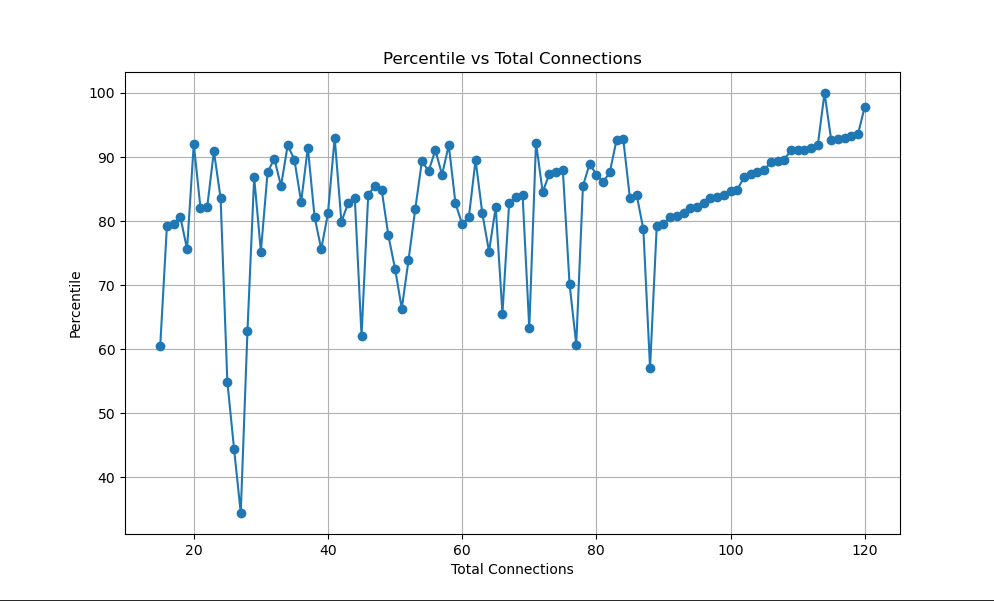
\includegraphics[width=0.75\textwidth]{Crest/Images/percentile_ghc.png}}
    \qquad
    \subfloat[Percentile of \emph{NYC\_abc}]{\label{fig:tinyCity}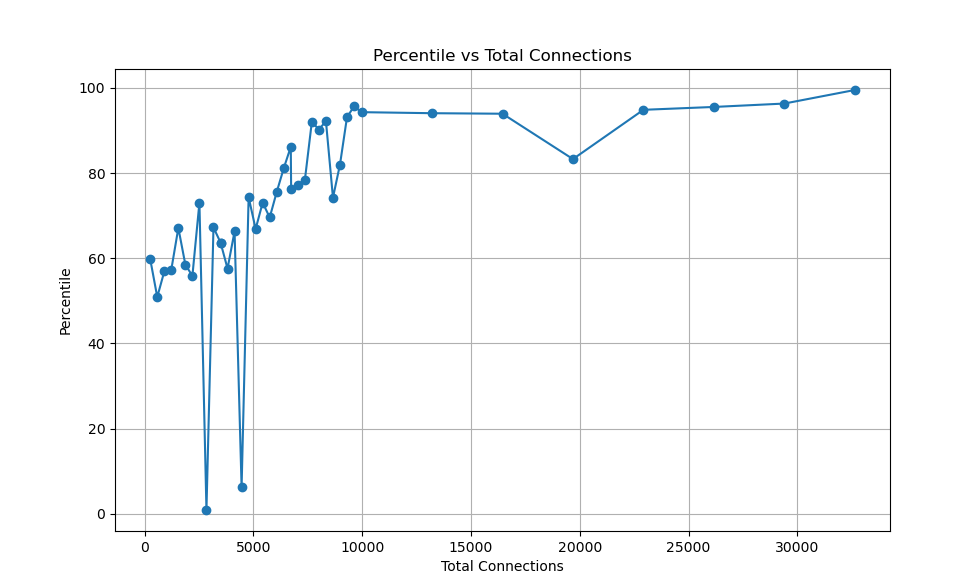
\includegraphics[width=0.75\textwidth]{Crest/Images/percentile_nyc.png}}
    \qquad
    \subfloat[Multi-objective Results for \emph{GHC\_abc}]{\label{fig:tinyCity}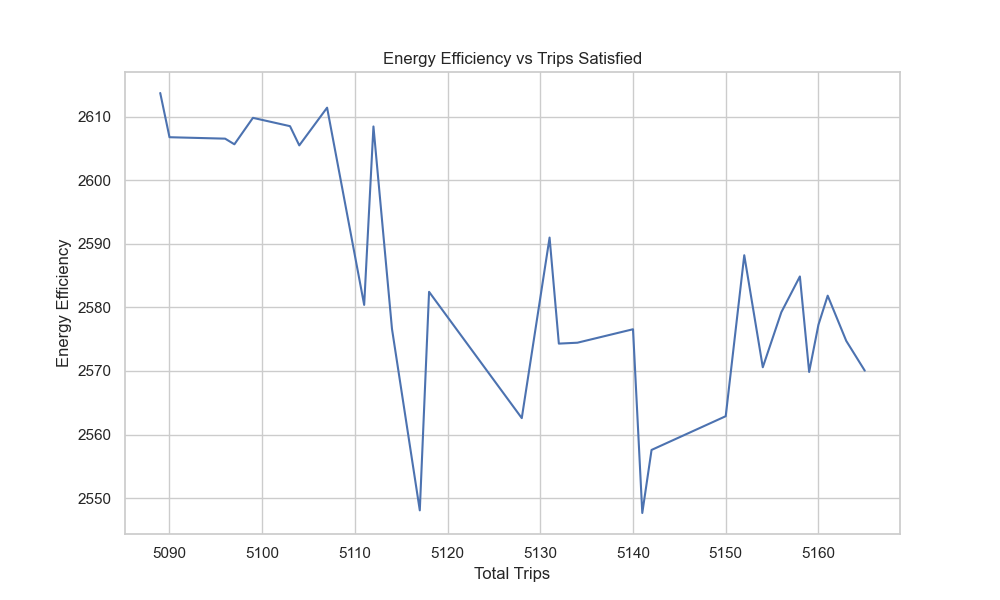
\includegraphics[width=0.75\textwidth]{Crest/Images/metropolis_energy_consumption_converge.png}}
    \caption{Performance Results}
    \label{fig:resultsFigure}
\end{figure}
Specifically, Figure \ref{fig:resultsFigure}(a) (resp. Figure \ref{fig:resultsFigure}(b)) presents the percentile of the
solution $qr$ when solving the instances of \emph{GHC\_abc} (resp. \emph{NYC\_abc}); results for the normal
distributions are omitted, as they are quite similar to the displayed ones.
The decentralised negotiation process carried out by the RL solution approach proves to find high quality solutions,
with $qr$ in a percentile of 60+ for all instances.
Moreover, it seems to be a trend that the higher the number of connections among SECs, the higher the $qr$
obtained, being able to find near optimal solutions when almost all connections are enabled.
A few outlier configurations are observed, with a temporary reduction in the increasing trend of $qr$.
This can be attributed to the $\epsilon$-greedy learning process. The SECs explore the environment to learn optimal policies that maximise the
expected rewards, which might lead to consecutive suboptimal actions that are hard to recover from afterwards.

As the total number of connections between SECs increases, two key trends emerge:

\begin{enumerate}
    \item \textbf{Improved Performance:} With more inter-SEC connections, the network becomes more flexible, providing additional pathways for vehicle exchanges. This structural redundancy allows the decentralised Q-Learning algorithm to better reallocate AEVs, resulting in solutions that converge closer to the centralised MILP-derived upper bound. In essence, increased connectivity reduces geographic or resource isolation, enabling SECs to balance their vehicle availability more effectively.

    \item \textbf{Reduced Variability:} The observed reduction in result variability as connections increase is attributed to the diminishing influence of initial allocation imbalances or specific network topologies. Sparse networks are more sensitive to initial conditions or local constraints, which can lead to higher solution variability. In contrast, well-connected networks offer more consistent reallocation opportunities across all SECs, stabilising performance outcomes.
\end{enumerate}

These findings align with general principles in network optimisation and multi-agent systems, where enhanced connectivity improves resource flow and system robustness, particularly under decentralised decision-making frameworks \cite{klapp2020decentralized}.

In terms of the multi-objective goal of the RL solution approach
(i.e., the number of TPs serviced vs the energy consumption of the AEVs)
Figure \ref{fig:resultsFigure}(c) indicates that the reward function contributes to a more stable energy consumption pattern as the number of connections among SECs increase.
This indicates that SECs with shorter average journey durations are favoured over those with longer travels, leading to enhanced energy efficiency.  Nonetheless, this prioritising necessitates meticulous evaluation.  Focussing on shorter travels can improve overall system efficiency by decreasing energy consumption per trip, but it may unintentionally harm groups whose mobility requirements naturally entail greater distances.  A balanced approach is essential: the system must pursue overall efficiency while maintaining service fairness among localities.  Future research should investigate strategies to dynamically modify this priority, taking into account both energy efficiency and equitable access to mobility services.
 %However, it is important to note that this value
%may further increase once more sophisticated vehicle-passenger routing algorithms are incorporated.

Finally, in terms of scalability, the RL solution approach
is able to solve each instance of each of the benchmarks in less than 15 seconds, with an average execution time
per instance of 10.57 seconds. This indicates that the
proposed approach is efficient and capable of handling very large instances (with thousands of trips and vehicles),
potentially making it suitable for its application to real-world scenarios.

\section{Effect of EV Fleet Size on Performance}
\label{sec:fleet_size_performance}
This section explores how varying the number of autonomous electric vehicles (AEVs) allocated to the system influences overall performance, particularly focusing on trip satisfaction and energy efficiency.

\subsection{Objective}
This section evaluates the impact the size of the AEV fleet has in terms of number of TPs being served and energy consumption. 

\subsection{Experimental Setup}
To study the impact of fleet size, the number of AEVs in the city are kept at 50\%, 100\%, and 150\% of the ones of the instances (\emph{GHC\_ai})(i.e., 200, 400 and 600 AEVs, respectively). 

The performance of the system is evaluated in terms of two primary metrics:
\begin{itemize}
    \item \textbf{Number of trips served}: The total number of TPs successfully allocated and served during the simulation.
    \item \textbf{Energy consumption}: The total energy consumed by the fleet to serve the trips.
\end{itemize}

Each configuration employs the RL-based solution approach, which involves 100 episodes. Each experiment used the identical hardware specified in Section \ref{sec:experimental_setup}.

% \subsection{Expected Outcome}
% The experiment is expected to provide insight into the impact of fleet size on the quality of the ride-sharing solution and the system's energy efficiency. Increasing the number of AEVs should initially result in more trips being served, but diminishing returns are expected after reaching a certain fleet size. This could indicate the optimal fleet size for the given city configuration.

\subsection{Results and Analysis}
Table \ref{tab:fleet_size_results} shows the results of the experiments, comparing the number of trips served and energy consumption across different fleet sizes. Figure \ref{fig:fleet_size_performance} shows a visual comparison of the outcomes.


\begin{table}[htbp]
    \centering
    \caption{Effect of EV Fleet Size on Performance}
    \label{tab:fleet_size_results}
    \begin{tabular}{|c|c|c|c|}
        \hline
        \textbf{Fleet} & \textbf{TP Served} & \textbf{Energy(units))} & \textbf{Energy Efficiency (TP/units)} \\
        \hline
        50\% Fleet  & 4,200 & 12,500 & 0.336 \\
        100\% Fleet  & 5,196 & 15,000 & 0.346 \\
        150\% Fleet & 5,250 & 17,500 & 0.300 \\
        \hline
    \end{tabular}
\end{table}

Table \ref{tab:fleet_size_results} show that, as the fleet size increases, so it does the number of TPs being served. However, in terms of energy efficiency, a peak is reached by the medium-sized AEVs fleet, for it to decrease when moving to the high-sized AEVs fleet.

This indicates that, while growing the fleet size enables for more trips to be served, the system eventually reaches a threshold of diminishing returns, at which adding more vehicles results is a less efficient use of energy.

\begin{figure}[htbp]
    \centering
    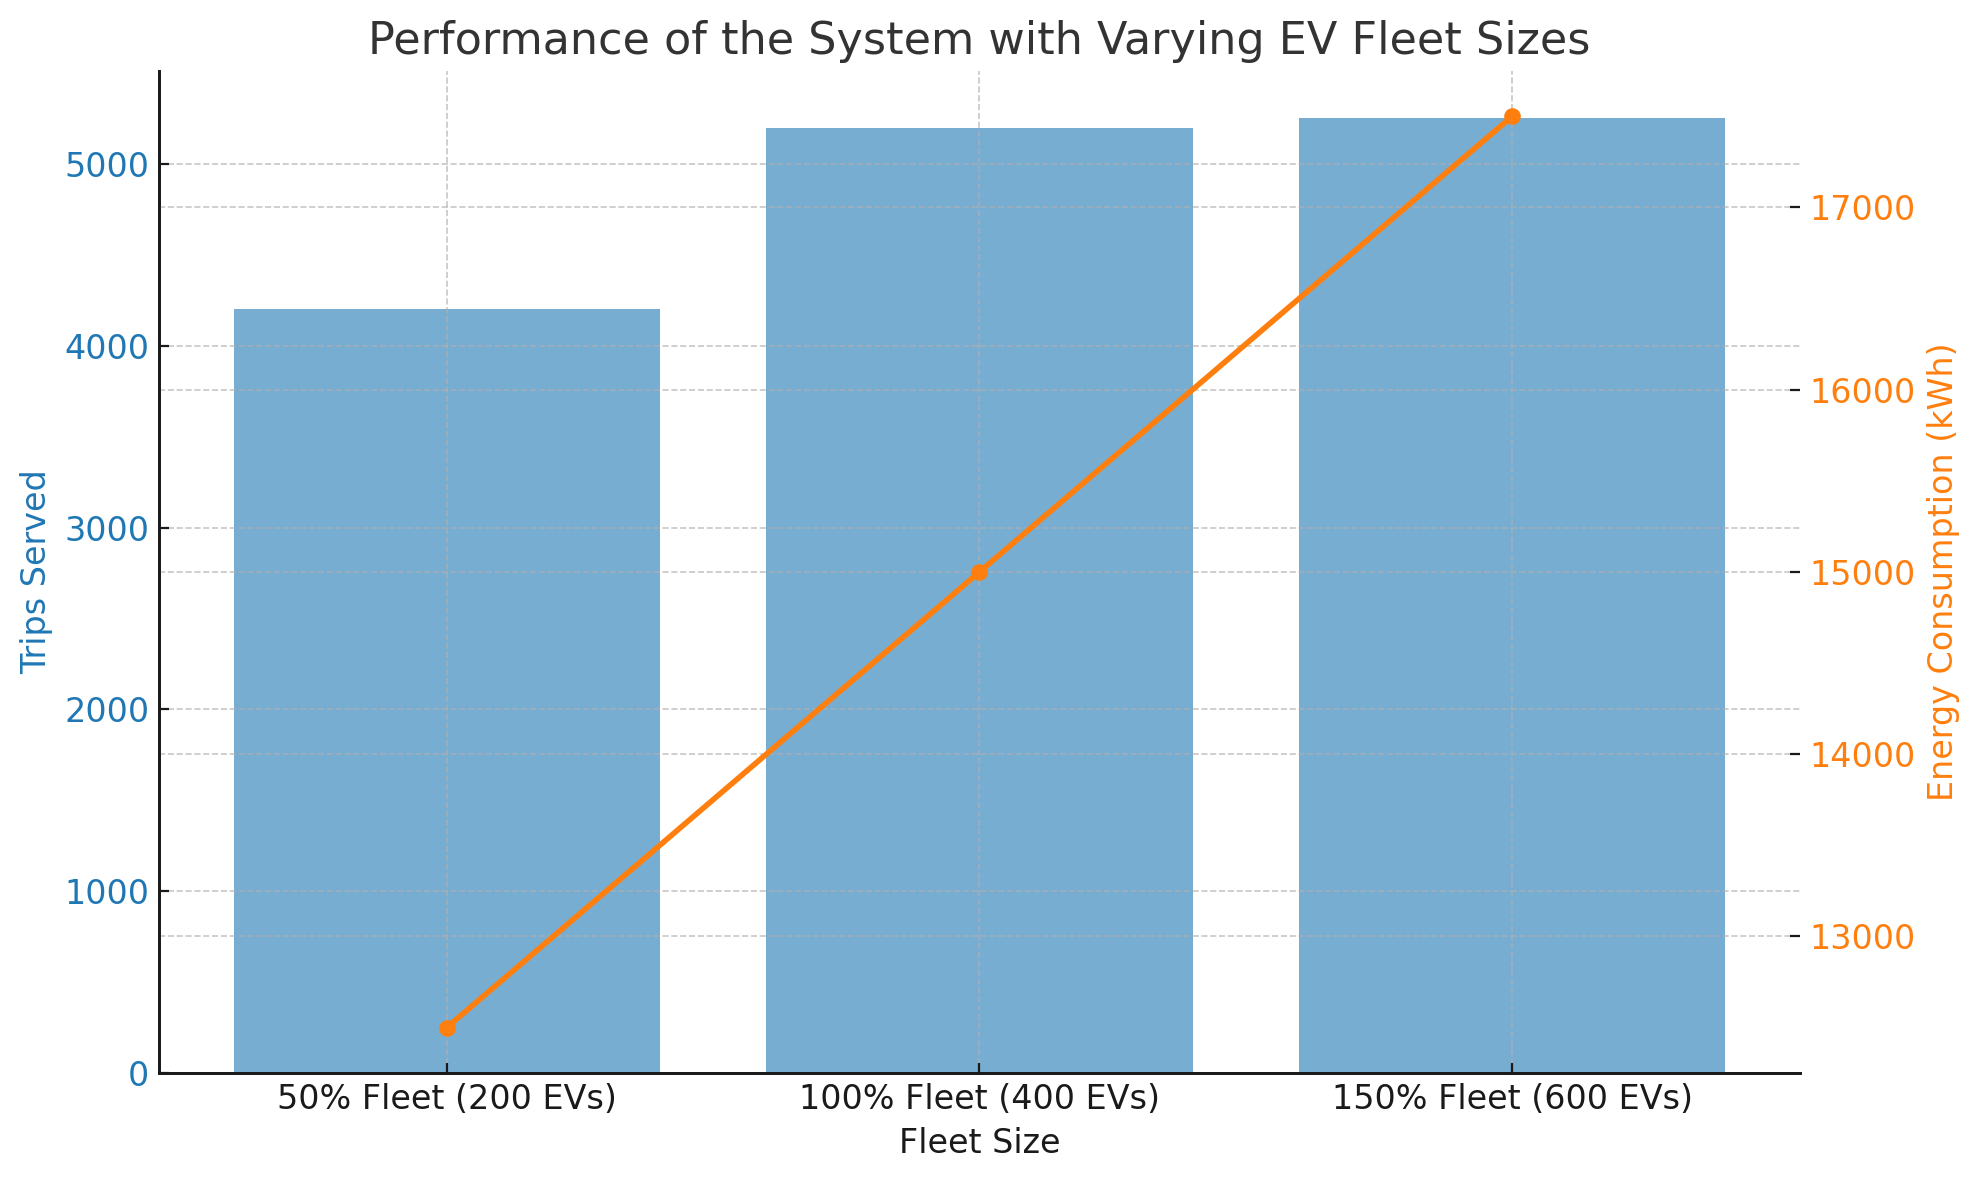
\includegraphics[width=0.75\textwidth]{Crest/Images/fleet_size_performance.png}
    \caption{Performance of the system with varying EV fleet sizes}
    \label{fig:fleet_size_performance}
\end{figure}


% \subsection{Conclusion}
The experimental results show that increasing the number of AEVs improves the total number of trips served, but only to a degree. Beyond this limit, the energy efficiency of the system declines. Further increases in fleet size result in declining returns and lower energy efficiency, which should be considered when scaling up EV fleets in real-world scenarios.

\section{Conclusions}
\label{sec:conclusion}

This chapter has presented the design, implementation and evaluation of the vehicle fleet allocation in a SEC-based
ride-sharing service, proposing a decentralised alternative
to the traditional central management in rapidly growing cities
(which are prone to dynamic urban environments and fluctuating travel demands).
On it, the independent SECs of the city compete for the allocation of AEVs resources,
which then they use to operate the TPs of its own neighbours via ride-sharing.
The vehicle allocation
problem has been formulated as a decentralised, iterative negotiation process among independent SECs,
where connected SECs decide the potential exchange of AEVs among them, based solely on their local information.
The underlying ride-sharing service operated by each SEC has been formulated using the ride-sharing model proposed in Chapter 3.
A solution approach to the problem tandem has been presented, using a Multi-Objective and Multi-Agent
RL algorithm, involving Deep Q-Learning with Graph Convolutional Networks, for SECs to
learn from previous negotiations.
The solution approach has been tested by aligning existing benchmarks (i.e. Google HashCode) and public
datasets (i.e. NYC taxis) to the proposed problem formulation, evaluating different SEC connectivity-levels
and transport request distributions.
The RL algorithm has proven to output high quality solutions in all cases, providing even near optimal solutions
when almost all SECs are able to exchange vehicles. Moreover, the RL algorithm has proven to scale well,
handling very large instances (with thousands of trips and vehicles) in just a few seconds, and therefore
potentially making it suitable for its application to real-world urban transportation systems. The complete code can be accessed via GitHub \cite{chapter4code}.

% The proposed approach provides multiple opportunities for future work.
% On the one hand, incorporating adaptive learning rates into the training procedure so that the model can adapt and fine-tune its parameters based on the current state of the system will be investigated to increase the overall learning efficacy.
% On the other hand, the ride-sharing service can be integrated with real-time traffic conditions, user preferences, and other dynamic variables, as well as the use of a dynamic charging infrastructure (consisting of both fixed and mobile charging stations), in order to promote more sustainable urban mobility.
\chapter{Reward-based Charging Schedule for a Community-based Ride-sharing Service}
\label{chapter5}

The models presented in chapters 3 and 4 have set the path for the intended carbon-neutral, scalable and decentralised ride-sharing service. In particular, Chapter 3 has explored the use of RES by the SECs, and the impact different AEV release approaches (e.g., START vs. SPREAD) has in the amount of TPs being served. Likewise, Chapter 4 examined the inter-relation of SECs, and the impact their negotiation process for allocating the AEV fleet has in the collective amount of TPs being served. 

The increasing integration of AAEVs in ride-sharing services introduces several complexities, particularly around the effective scheduling of charging sessions to maintain uninterrupted service availability \cite{energydatamanagement}. Current solutions often fall short in managing these challenges, either due to a lack of scalability, inefficient charging coordination, or limited consideration of SEC dynamics \cite{boasso2021sec}. Therefore, this chapter expands the key features of carbon neutrality and SEC interrelation by designing, implementing and evaluating a reward-based, intelligent charging scheduling to be integrated to the ride-sharing service. 

The new model sees each SEC owning a number of Charging Stations (CSs), and it RES-generated energy being split into (i) the energy used to release its own AAEVs and (ii) the energy used to re-charge already operative AAEVs. The new model exploits the inter-relation of SECs, enabling (1) host TPs to be served by an AEV of a different SEC, and (2) such AAEVs to re-charge their batteries in a host CSs in return. This charging scheduler involves a sophisticated decision-making process that accounts for multiple factors critical to the sustainable operation of the ride-sharing service. These factors include the proximity and waiting times of available CSs, the potential for service interruptions due to charging, and the dynamic re-allocation of AAEVs based on real-time assessments of energy consumption and vehicle availability. Additionally, the algorithm incorporates the flexibility to modify charging schedules dynamically by considering the collective prospects of multiple AAEVs. Overall, the charging scheduler aims to increase the robustness of the ride-sharing service, maximising its service across the entire time horizon. 

As with previous models, the charging scheduler is evaluated by aligning existing benchmarks (i.e. Google HashCode) and public datasets (i.e. NYC taxis) to the proposed problem formulation, simulating a variety of operational scenarios.

The chapter is organised as follows: Section \ref{sec:problem_definition} formalises the problem and Section \ref{sec:solution_approach} details the solution approach. Next, Section 5.3 presents an overall evaluation, with sections 5.4 to 5.7 then focusing on specific aspects, such as a comparison with baseline algorithms, the impact of charging speed, RES availability and TPs flexibility.  Finally, Section \ref{sec:conclusions_and_future_work} presents the main conclusions.


\section{Problem Definition}
\label{sec:problem_definition}

This section formalises the problem for integrating a reward-based, intelligent charging scheduling to the ride-sharing service defined in chapters 3 and 4. The new model integrates passenger allocation and re-routing constraints as both the TPs and the number of available vehicles evolve during a simulated time horizon. Aligning with the original formulation from Chapter 3, the ride-sharing service aims to maximise the number of TPs served and is designed to be highly scalable for large cities.

To better discuss the problem, its main features are enumerated here again, together with the novel features for the charging scheduler:
\begin{itemize}
    \item The grid dimensions of the city $c_r$, $c_c$ and the time horizon for the simulation $th$.Manhattan distances among the locations of the city are assumed.
    \[
    (c_r, c_c, th)
    \]
    \item A set $S$ of SECs, each with an id $s_{id}$, a location in the city $s_x$, $s_y$, a lexicographically ordered list of the vehicles belonging to it $s_E$, and the number of vehicles ready at the start of the simulation $s_R$.
    \[
    (s_{id}, s_x, s_y, s_R) \forall s \in S
    \]
    \item A set $E$ of AEVs, each with an id $e_{id}$, the id of the SEC it belongs to $s_{id}$, and its battery and passenger capacities ($e_{bc}$ and $e_{pc}$). A mapping from $E$ to $S$ is assumed, such that each $e_{id}$ belongs to one $s_{id}$. All AEVs are available at the start of the simulation.
    \[
    (s_{id}, e_{id}, e_{bc}, e_{pc}) \forall e \in E
    \]
    \item A set $T$ of TPs (TPs), each with an id $t_{id}$, its pick-up and drop-off locations $t_{px}, t_{py}, t_{dx}, t_{dy}$, and time windows $t_{ep}, t_{lp}, t_{ed}, t_{ld}$. Each TP includes a weight parameter $t_{w}$ indicating the importance of the TP. $t_{sid}$ id of the SEC $t_{id}$ is originating from. 
    \[
    (t_{id}, t_{px}, t_{py}, t_{dx}, t_{dy}, t_{ep}, t_{lp}, t_{ed}, t_{ld}, t_{w}, t_{sid}) \forall t \in T
    \]
    \item A set of charging stations (CSs) within the SECs, each represented by:
    \[
    (cs_{id}, s_{id}, cs_x, cs_y, cs_k, cs_{bn}) \forall c \in \mathcal{C}
    \]
    where $cs_{id}$ is the charging station ID, $s_{id}$ is the SEC ID, $cs_x$ and $cs_y$ are the coordinates, $cs_k$ is the queue limit which is the maximum number of AEVs that can charge at a charging station at a given same time, and $cs_{bn}$ is the charging rate per unit time which is used to compute the charging duration of an EV.
\end{itemize}

\subsection{Constraints}

The problem involves several key constraints that ensure the system operates efficiently and meets its objectives.

\begin{enumerate}
    \item \textbf{Trip Allocation Constraints:} A TP $t_{id}$ is allocated to an EV $e_{id}$ if the vehicle can meet the time-windows and capacity requirements:
    \[
    (e_{pc} \geq t_w \wedge e_{bc} \geq \text{required energy})
    \]
    This constraint ensures that each EV can handle the passenger load and has sufficient battery capacity to complete the trip.

    \item \textbf{Charging Constraints:} An EV is directed to a charging station when its battery level falls below a threshold $\beta$ or is \textit{idle} for the charging duration:
    \[
    [(e_{bc} \leq \beta) \wedge (e_{pc} \equiv 0)] \vee (m_i(TL_i) \equiv \text{idle})
    \]
    This constraint ensures that AEVs maintain sufficient battery levels and utilise idle times effectively for charging.

    \item \textbf{Reward $I$:} To promote inter-community service efficiency, AEVs receive a reward for serving trip petitions ($TPs$) originating from neighbouring SECs. Specifically, the reward gained by an AEV $e_{id}$ from serving a neighbouring TP $t_{id}$ is equal to the corresponding TP weight $t_{w}$:

        \[
        I_{e_{id}} = \sum_{t \in \mathcal{T}_{\text{neighboring}}} t_{w}
        \]
        
    The inclusion of this reward mechanism enhances system-level coordination in the decentralised scheduling process. Although SECs are assumed to operate under a cooperative framework, individual AEVs act as distributed agents making local decisions based on limited information. In such settings, reward structures serve as an indirect incentive alignment tool, guiding vehicle-level decision-making toward globally beneficial behaviours.
    
    In practical terms, the reward $I$ is integrated into the scheduling algorithm as part of the decision-making process. When multiple trip options are available, AEVs evaluate potential assignments based not only on travel distance or timing constraints but also on accumulated reward potential, prioritising trips that strengthen inter-SEC collaboration.
    
    The reward system thus functions as a lightweight reinforcement mechanism that:
    
    \begin{itemize}
        \item Encourages AEVs to serve TPs beyond their home SECs, improving geographic service coverage.
        \item Increases the overall number of TPs served, particularly in scenarios where local SEC capacity alone is insufficient.
        \item Provides a scalable, decentralised means of improving system efficiency, even in cooperative, non-competitive environments.
    \end{itemize}
    
    While Chapter 4 assumes cooperative SEC behaviour, the dynamic, decentralised nature of vehicle operations still benefits from  reward mechanisms to align individual vehicle actions with broader service objectives.
\end{enumerate}

\subsection{Solution Representation}
The solution to the problem is represented by the same two sets Alloc and Sched as in Chapter 3.

\begin{itemize}
    \item A set $Alloc$, representing an allocation mapping from $T$ to $E$.
    \[
    \forall t \in T \text{ } Alloc[t_{id}] = 
    \begin{cases}
        e_{id},  \text{if }  t_{id} \text{ is allocated to } e_{id}\\
        -1,  \text{otherwise}
    \end{cases}
    \]
    \item A set $Sched$, representing a scheduling mapping from $E$ to its sequence of movements (in chronological order) over the entire time horizon.
    \[
    \forall e \in E \text{ } Sched[e_{id}] = (m_0, m_1, \ldots, m_{n-1})
    \]
    Each movement $m_i$ of a vehicle is represented the same way as in Chapter 3, with special novel movement tags for charging actions
    \begin{align*}
    m_i \equiv \{ (TA_i, TB_i, AX_i, AY_i, BX_i, BY_i, PS_i, \\
        PE_i, ES_i, EE_i, TL_i, LW_i, TD_i) \}
    \end{align*}
    with: 
    \begin{itemize}
        \item $TA_i$ (resp. $TB_i$) represent the start time (resp. end time) of $m_i$.
        \item $AX_i$ and $AY_i$ (resp. $BX_i$ and $BY_i$) represent the coordinates of the vehicle at the start (resp. end) of $m_i$.
        \item $PS_i$ (resp. $PE_i$) represents the number of passengers in the vehicle at the start time (resp. end time) of $m_i$.
        \item $ES_i$ (resp. $EE_i$) represents the battery left in the vehicle at the start time (resp. end time) of $m_i$.
        \item $TL_i$ represents a label to identify the purpose of the trip.
        \begin{itemize}
            \item A movement for picking-up (resp. dropping off) the passenger of $t_{id}$ is marked as $+t_{id}$ (resp. $-t_{id}$).
            \item A charging movement is marked as $charge$. $+charge$ indicates charging at a SEC and $-charge$ indicates the journey to the charging station.
            \item A waiting movement is marked $wait$ indicating the wait time at a CS prior to charging.
        \end{itemize}
        \item $LW_i$ represents the leeway of the movement, i.e., the maximum delay that could be applied to the movement while still accomplishing the intended action.
        \item $TD_i$ represents the movement duration.
    \end{itemize}
\end{itemize}

\section{Solution Approach}
\label{sec:solution_approach}

This section presents the solution approach for the ride-sharing service. It consists of the integration of a newly developed charging scheduling algorithm into the previously developed trip allocation and vehicle routing algorithm of Chapter 3. 

\subsection{Vehicle Routing Algorithm}
\label{vehicle-allocation-algorithm}
The TP allocation and vehicle routing of the ride-sharing services builds upon the reactive ride-sharing algorithm previously developed in Chapter 3. 

One novel aspect of the current model is its proactiveness, as the algorithm is aware of the full set of TPs arising over the simulated time horizon, enabling it to take all TPs into account for decision-making. This contrasts with the reactive nature of the original model presented in Chapter 3, which dynamically re-allocated and re-scheduled AEVs as each new TP was introduced. The proactive simulation algorithm prioritises serving TPs ($t_{id}$) with the highest trip weights ($t_w$) first. It iterates through each $e_{id}$ in the set of AEVs, attempting to allocate the trip to the vehicle by dynamically re-routing its schedule. Once a trip is successfully allocated to a vehicle, the search stops. If no vehicle can allocate the trip, the attempt is considered unsuccessful.

Algorithm 4 presents the pseudo-code for the vehicle allocation and routing of the ride-sharing service. The function `Allocate' is the same as in Algorithm 1 in Chapter 3, and is provided here again for clarity purposes. The `Proactive\_Simulation' represents the modification w.r.t. Algorithm 1 in Chapter 3.

\begin{algorithm}
\caption{Proactive Ride-sharing Algorithm}
\begin{algorithmic}
\Function{allocate}{$e$, $t$, $Alloc[t]$, $Sched[e]$}
    \State $is\_allocated \gets false$
    \State $m \equiv [ m_0, \ldots, m_{k-1} ] \gets copy(Sched[e])$
    \For{$i \in 0, \ldots, k-1$}
        \If{$pick\_up(m, t, i)$}
            \State $m \gets [ m_0, \ldots, m_i', m_{i+1}', \ldots, m_{r-1}' ]$
            \For{$j \in i+1, \ldots, r-1$}
                \If{$drop\_off(m, t, j)$}
                    \State $m \gets [ m_0, \ldots, m_j'', m_{j+1}'', \ldots, m_{w-1}'' ]$
                    \If{$ret\_sec(m, w-1)$}
                        \State $m \gets [ m_0, \ldots, m_{w-1}'', m_w'' ]$
                        \State $(Alloc[t], Sched[e]) \gets (e, m)$
                        \State $is\_allocated \gets true$
                    \EndIf
                    \State \textbf{break}
                \EndIf
            \EndFor
            \State \textbf{break}
        \EndIf
    \EndFor
    \Return $is\_allocated$
\EndFunction
\\ \hrulefill
\Function{proactive\_simulation}{$S$, $E$, $T$, $th$}
    \State $(Alloc, Sched) \gets init(S, E, T, th)$
    \For{$t \in sortedByTripWeight(T)$}
        \For{$e \in E$}
            \If{$allocate(e, t, Alloc[t], Sched[e])$}
                \State \textbf{break}
            \EndIf
        \EndFor
    \EndFor
    \Return $(Alloc, Sched)$
\EndFunction
\end{algorithmic}
\end{algorithm}

%%%%%%%%%%%%%%%%%%%%%%%%%%%%%%%%%%%%%%%%%%%%%
% Subsection Charging Scheduling Mechanism
%%%%%%%%%%%%%%%%%%%%%%%%%%%%%%%%%%%%%%%%%%%%%
\subsection{Vehicle Charging Algorithm}

To integrate EV charging into the ride-sharing service, the following process is adopted. 

\subsubsection{Initial Scheduling}

Let \( E \) be the set of AEVs and \( T \) be the set of TPs (TPs). The vehicle routing algorithm computes the initial schedules for all AEVs, denoted as \( S_e \) for each \( e \in E \). Each schedule \( S_e \) includes a sequence of movements \( m_i \) with associated pick-up and drop-off times \( TA_i \) and \( TB_i \), locations \( (AX_i, AY_i) \) and \( (BX_i, BY_i) \), battery levels \( ES_i \) and \( EE_i \), and other parameters, ensuring all time windows and capacity constraints are met.

\subsubsection{Optimal Charging Points}

Given the initial schedules \( S_e \), the vehicle charging algorithm identifies optimal charging points within the schedule of each EV based on several factors:

\begin{enumerate}
    \item \textbf{Current Battery Capacity:} Let \( \beta \) be the battery threshold. Prioritise AEVs with \( e_{bc} < \beta \).
    \[
    \text{Priority}(e) \propto \left( \frac{1}{e_{bc}} \right)
    \]
    
    \item \textbf{Incentives Earned:} Let \( I_{s_{id}} \) be the incentives accumulated by SEC \( s_{id} \). Incentives influence the charging priority:
    \[
    \text{Priority}(e) \propto I_{s_{id}} \text{ for } e \in s_E
    \]
    
    \item \textbf{Proximity to Charging Stations (CS):} Let \( d(e, cs) \) be the Manhattan distance between EV \( e \) and charging station \( cs \). AEVs closer to a CS are preferred:
    \[
    \text{Priority}(e, cs) \propto \left( \frac{1}{d(e, cs)} \right)
    \]
    
    \item \textbf{Future Trip Potential:} Let \( V_e(t) \) be the potential number of trips an EV \( e \) can serve from the time it finishes charging \( t \) to the end of the time horizon \( th \). This is estimated by running the ride-sharing algorithm for the remaining time units:
    \[
    V_e(t) = \sum_{i=t}^{th} \left( \text{Weight of trips served by } e \text{ at time } i \right)
    \]
\end{enumerate}

% \subsubsection{Reward Mechanism}

% Each time an EV \( e \) serves a petition \( t \) from a neighboring SEC, its home SEC \( s_{id} \) gains incentives \( I_{s_{id}} \). These incentives are used to reward AEVs for charging sessions, encouraging AEVs to serve neighboring SECs:
% \[
% I_{s_{id}} = \sum_{t \in T_{\text{neighboring}}} t_w
% \]

\subsubsection{Eviction Policy}
An EV \( e_1 \) currently charging at a CS can be evicted if a newly arriving EV \( e_2 \) demonstrates a higher potential to serve additional trip petitions once recharged. The motivation for incorporating this eviction policy is grounded in the system-wide objective of maximising TP satisfaction, particularly in scenarios with constrained charging infrastructure or limited renewable energy availability.

CSs within SECs operate as bottlenecks in the overall ride-sharing service. In dynamic environments with fluctuating trip demands and decentralised AEV operations, the static allocation of charging slots based solely on arrival time can lead to suboptimal outcomes. Specifically, low-priority or underutilised AEVs occupying CSs may inadvertently block vehicles with greater potential to fulfill trip petitions, undermining system efficiency.
Let \( \tau \) be the time unit and \( d_{\text{charge}} \) be the charging duration. The ride-sharing algorithm is run for \( e_1 \) from \( \tau + d_{\text{charge}} \) to \( th \) and for \( e_2 \) from \( \tau \) to \( th \). EV \( e_1 \) is evicted if:
\[
V_{e_2}(\tau + d_{\text{charge}}) > V_{e_1}(\tau + d_{\text{charge}})
\]
Figure \ref{fig:eviction_policy} shows how the vehicle routes are taken into account to compute the eviction policy. 
\begin{figure}[h]
  \vspace{-0.2cm}
  \centering
  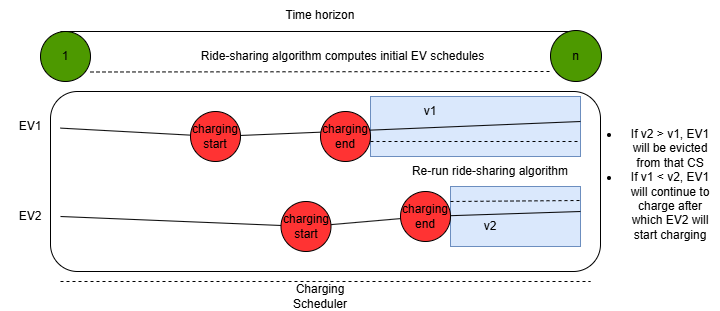
\includegraphics[width=7.5cm]{Crest/Images/eviction_policy.png}
  \caption{Eviction Policy}
  \label{fig:eviction_policy}
  \vspace{-0.1cm}
\end{figure}

\subsubsection{Iterative Process}

The vehicle charging algorithm iteratively refines battery re-charges for AEVs until no further improvements in the overall number of trips being served are observed. A maximum number of iterations \( n \) is given as input parameter. The follow 3-steps process is then performed until either the algorithm converges or reaches the maximum number of iterations.    %The process ensures optimal scheduling and resource utilisation:
\[
\text{Repeat until convergence:}
\begin{cases}
    \text{Run ride-sharing algorithm} \\
    \text{Update EV schedules} \\
    \text{Update charging decisions}
\end{cases}
\]
This iterative process aims for the overall system performance to continually improve, with the goal of maximising the number of TPs served while maintaining efficient resource allocation. Figure \ref{fig:flowchart} illustrates the interaction between the vehicle routing algorithm and the vehicle charging algorithm.
\begin{figure}[b]
  \vspace{-0.2cm}
  \centering
  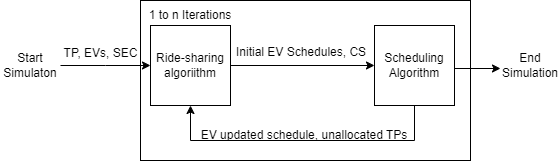
\includegraphics[width=7.5cm]{Crest/Images/flowchart.png}
  \caption{Interaction between Charging Scheduler and Ride-sharing Algorithms}
  \label{fig:flowchart}
  \vspace{-0.1cm}
\end{figure}

Algorithm 5 presents the pseudo-code for the vehicle charging of the ride-sharing service. Overall, key enhancements made to the ride-sharing service from its original implementation in Chapter 3 are:
\begin{itemize}
    \item Proactive scheduling to anticipate future TPs.
    \item Reward mechanisms to encourage strategic trip fulfillment.
    \item Strategic selection and management of CSs.
    \item Dynamic charging and eviction decisions based on potential trips being served.
    \item Iterative improvement processes to continually optimise system performance.
\end{itemize}

%%% Algorithm 2



\begin{algorithm}
\caption{Charging Scheduling Algorithm}
\begin{algorithmic}
\Function{Charging\_Scheduler}{$S$, $E$, $T$, $th$}

    \State $(Alloc, Sched) \gets init(S, E, T, th)$
    \State $X \gets \text{Sum  weights  TPs served in T } Alloc$
    \State $I_E \gets \text{sum  weights TPs served in neighboring SECs }$
    \State $no\_improvement\_count \gets 0$



    \While{$no\_improvement\_count < T$}
        \State $candidates \gets \text{FilterCandidates}(E, Sched)$
        \State $best\_candidate \gets \text{SelectBestCandidate}(candidates)$

        \If{$best\_candidate \neq \text{None}$}
            \State $\text{SendToCharge(best\_candidate)}$
            \State $sched \gets \text{RecomputeSchedule(best\_candidate.EV, Sched)}$
            \State $new\_X \gets \text{number of TPs being served in } Alloc$
            \If{$new\_X > X$}
                \State $X \gets new\_X$
                \State $no\_improvement\_count \gets 0$
            \Else
                \State $no\_improvement\_count \gets no\_improvement\_count + 1$
            \EndIf
        \Else
            \State $no\_improvement\_count \gets no\_improvement\_count + 1$
        \EndIf
    \EndWhile

    \Return $(Alloc, Sched)$
\EndFunction
\end{algorithmic}
\end{algorithm}

\section{Overall Evaluation}
\label{sec:evaluation}

This section assesses the charging scheduling algorithm proposed for a carbon-neutral, community-based, proactive ride-sharing service. The parameterised instance generator of Chapter 3 has been re-used to align existing benchmarks (i.e., Google Hashcode) and public datasets (i.e., NYC taxis) to the proposed problem formulation and to enable testing of the solution under various configurations.

\subsection{Experimental Setup}
The key parameters for the experiments are as follows:
\begin{enumerate}
    \item \textbf{Hashcode Dataset:} 10,000 TPs and 400 AEVs.
    \item \textbf{NYC Dataset:} 50,000 TPs and 1,000 AEVs.
\end{enumerate}

The key factors being explored are:
\begin{enumerate}
    \item \textbf{Number of SECs:} Different configurations of the number of SECs.
    \item \textbf{Energy Factor:} The energy available at each SEC.
    \item \textbf{Flexibility:} The flexibility in the pick-up and drop-off time windows of each TP.
\end{enumerate}

These factors lead to a wide range of results in terms of the overall number of trips being served, as shown in Table \ref{tab:datasets}. To analyse the charging algorithm, three instances of the Google Hashcode dataset are selected, as well as one instance of the New York City dataset to explore the scalability of the algorithm. 

The GHC dataset represents a synthetic, scalable benchmark environment specifically designed for algorithm stress-testing under controlled conditions. These controlled variations allow for a comprehensive sensitivity analysis of the proposed algorithms across different operational scenarios. In contrast, the NYC dataset represents a real-world, irregular urban topology derived from actual taxi trip data. Due to the inherent complexity, heterogeneity, and limited control over spatial and temporal patterns in this dataset, only one baseline configuration is applied. This configuration is selected to reflect a realistic, high-density urban mobility environment, providing a validity check for the proposed approach.

Table \ref{tab:datasets} shows the top results obtained from the \cite{smartgreens} ride-sharing solution where charging was not considered. 


\begin{table}[htbp]
\caption{Hashcode and NYC Instances}
\begin{center}
\begin{tabular}{|c|c|}
\hline
\textbf{Hashcode Instances Configuration}&\textbf{Trips Served}\\
\hline
GH01 Flexibility - 50\%; SECs - 16; Energy Factor - 2.0 & $\equiv$ 89.69\% \\
GH02 Flexibility - 25\%; SECs - 16; Energy Factor - 1.0 & $\equiv$ 51.19\% \\
GH03 Flexibility - 10\%; SECs - 1; Energy Factor - 2.0 & $\equiv$ 0.06\% \\
TPs = 10000, EV = 400 & \\
\hline
\textbf{NYC Instance Configuration}&\textbf{Trips Served}\\
\hline
NY01 Flexibility - 50\%; SECs - 16; Energy Factor - 2.0 & $\equiv$ 88.5\% \\
TPs = 50000, EV = 1000 & \\
\hline
\end{tabular}
\label{tab:datasets}
\end{center}
\end{table}


% \subsection{Results and Analysis}

All experiments are conducted on a machine with the following specifications: Mac OS Ventura, Intel i7 Quad Core 2.3Ghz processor and 16GB RAM memory. %The complete code can be accessed via GitHub \cite{rewardcharging}. 
The next subsections analyse the results. 

\subsection{Impact of Iterations on Trip Served}

The number of trips served increases significantly with the number of iterations across all instances tested. In the Hashcode dataset (GH01), under conditions of 50\% flexibility, 16 SECs, and an energy factor of 2.0, the percentage of trips served rose from 89.69\% (without any charging infrastructure) to 98.66\% (with charging infrastructure) after ten iterations, reflecting a 10\% improvement. Similarly, the NYC dataset (NY01) shows an improvement from 88.5\% to 96.5\% with iterations. 

However, differences are observed across instances: for GH02 and GH03, where TPs exhibit lower flexibility, the number of trips served saturates much earlier, with only marginal improvements after 3--5 iterations. This indicates that higher trip flexibility allows the system to benefit more significantly from the charging scheduling algorithm, whereas low-flexibility instances reach an operational limit quickly. 

Overall, the algorithm demonstrates excellent scalability, solving large instances of up to 10,000 trips in approximately two minutes and handling up to 50,000 trips in about twenty minutes (see Figure~\ref{fig:iterations} and Table~\ref{tab:trip_satisfaction}). 

Figure \ref{fig:energy_charging_utilise}  and table \ref{tab:energy_utilization_tab} shows the energy utilisation efficiency across CSs. It illustrates the percentage of energy left at CSs over iterations for all test instances. As shown, the algorithm effectively maximises energy usage, with the remaining energy converging to near-zero levels for GH01, GH02, and NY01 within ten iterations. This indicates optimal exploitation of renewable energy resources in these scenarios. In contrast, instance GH03 consistently maintains high levels of unused energy (close to 100\%), which aligns with its restrictive condition of low trip flexibility, limiting vehicle dispatch requirements.

\begin{figure}[h]
  \vspace{-0.2cm}
  \centering
  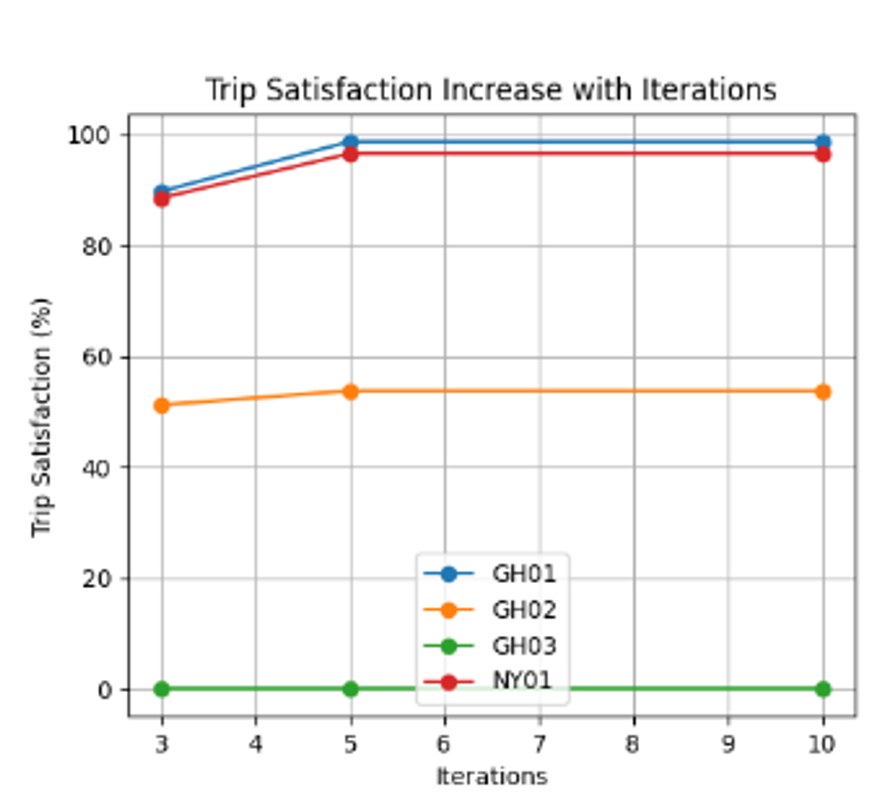
\includegraphics[scale=0.3]{Crest/Images/iterations.png}
  \caption{Number of Trips being Served over Iterations}
  \label{fig:iterations}
  \vspace{-0.1cm}
\end{figure}

\begin{figure}[h]
  \vspace{-0.2cm}
  \centering
  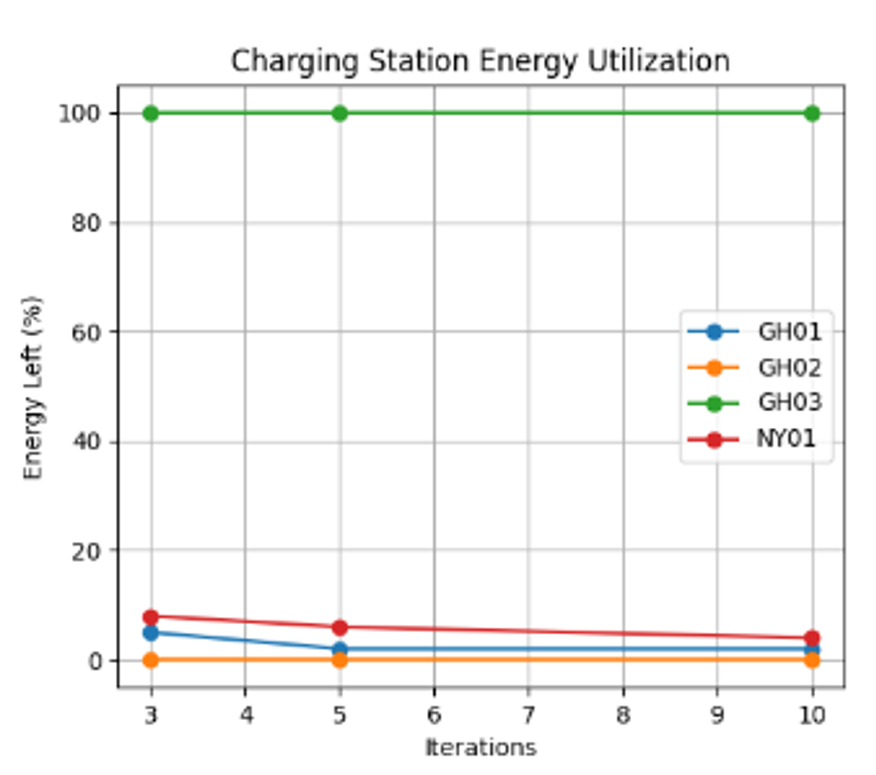
\includegraphics[scale=0.3]{Crest/Images/energy_charging_utilise.png}
  \caption{Energy Utilisation Efficiency}
  \label{fig:energy_charging_utilise}
  \vspace{-0.1cm}
\end{figure}


\begin{table}[htbp]
\caption{Improvement(\%) of Trips Served over Iterations}
\begin{center}
\begin{tabular}{|c|c|c|c|}
\hline
\textbf{Dataset} & \textbf{ Iterations} & \textbf{Improvement (\%)} & \textbf{Time (mins)} \\
\hline
GH01 & 3 & 8 & 7 \\
GH02 & 3 & 2 & 7 \\
GH03 & 3 & 0 & 2 \\
NY01 & 3 & 2.5 & 7 \\
GH01 & 5 & 10 & 10 \\
GH02 & 5 & 2 & 10 \\
GH03 & 5 & 0 & 2 \\
NY01 & 5 & 8 & 12 \\
GH01 & 10 & 10 & 10 \\
GH02 & 10 & 2 & 12 \\
GH03 & 10 & 0 & 2 \\
NY01 & 10 & 8 & 20 \\
\hline
\end{tabular}
\label{tab:trip_satisfaction}
\end{center}
\end{table}



\subsection{Charging Station Energy Utilisation}
Each SEC consists of a charging station with limited energy availability, denoted by the energy factor, which was efficiently managed by the algorithm. The number of times an AEV charged at a CS varied depending upon the initial trip allocation of the AEV and the reward procurement. 

CSs located near regions with high trip density became more in demand, as they offered shorter detours for AEVs with low battery levels. Furthermore, CSs positioned close to the boundaries between SECs experienced higher usage, as inter-SEC trips leveraged nearby charging infrastructure to minimise downtime. For instance, in the Hashcode dataset, the energy of each CS was utilised effectively, contributing to a higher number of TPs being served.

A more detailed analysis of spatial charging station demand patterns is provided in the following sections of this chapter.

Figure \ref{fig:avg_charges} shows the average number of charges per EV at different battery capacities for one of the Hashcode dataset instances (GH01). The x-axis represents the battery capacity, while the y-axis shows the average number of charges required. Higher battery capacities result in fewer charges, indicating more efficient energy use.
\begin{figure}[h]
  \vspace{-0.2cm}
  \centering
  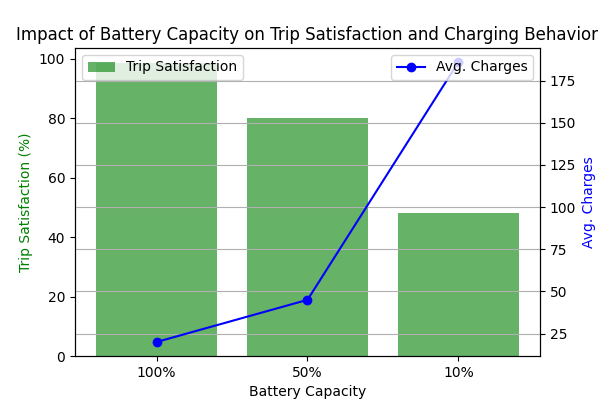
\includegraphics[scale=0.40]{Crest/Images/tripsatisfied_vs_battery.png}
  \caption{Impact of battery capacity on charging behavior}
  \label{fig:avg_charges}
  \vspace{-0.1cm}
\end{figure}

Table~\ref{tab:energy_utilization_tab} provides detailed results for the charging station energy utilisation across different datasets and iterations. The average number of charges per AEV and the remaining energy percentage at each SEC after the simulation is completed. 
\begin{table}[h]
\caption{Charging Station Energy Utilisation}
\begin{center}
\begin{tabular}{|c|c|c|c|c|}
\hline
\textbf{Dataset} & \textbf{SECs} & \textbf{Avg. Charges} & \textbf{Energy Left (\%)} & \textbf{Iterations} \\
\hline
GH01 & 16 & -- & 45 & 0 \\
GH01 & 16 & 15 & 5 & 3 \\
GH01 & 16 & 18 & 2 & 5 \\
GH01 & 16 & 20 & 2 & 10 \\
NY01 & 16 & -- & 50 & 0 \\
NY01 & 16 & 35 & 8 & 3 \\
NY01 & 16 & 45 & 6 & 5 \\
NY01 & 16 & 50 & 4 & 10 \\
\hline
\end{tabular}
\label{tab:energy_utilization_tab}
\end{center}
\end{table}


Before applying the charging scheduler (i.e., at 0 iterations), a substantial portion of energy remained unused --- approximately 45\% for GH01 and 50\% for NY01. After integrating the charging scheduler and running the iterative optimisation, the remaining total energy dropped significantly to as low as 2--4\%, reflecting highly efficient resource management. It is important to clarify here that the objective of the proposed charging scheduler is not to maximise energy consumption per se, but to maximise the number of trip petitions served while operating within the available renewable energy constraints.These results clearly demonstrate the impact and effectiveness of the charging scheduling algorithm in maximising the use of available renewable energy resources.


\subsection{Impact of Battery Capacity on Trip Served and Charging Behavior}

The impact of different battery capacities on trips served and charging behavior is significant. Table~\ref{tab:battery_capacity} summarises the performance across different battery capacities. AEVs with higher battery capacities required fewer charging sessions, leading to higher trip service rates. Conversely, AEVs with lower battery capacities needed to charge much more frequently, which disrupted their schedules and reduced the overall number of trips served.

\begin{table}[htbp]
\caption{Impact of Battery Capacity}
\begin{center}
\begin{tabular}{|c|c|c|c|}
\hline
\textbf{Data} & \textbf{Battery} & \textbf{Trips Served (\%)} & \textbf{Avg. Re-Charges/AEV} \\
\hline
GH01 & 100 & 98.66 & 20 \\
GH01 & 50 & 80.00 & 45 \\
GH01 & 10 & 48.00 & 186 \\
NY01 & 100 & 98.66 & 256 \\
NY01 & 50 & 80.00 & 505 \\
NY01 & 10 & 48.00 & 1290 \\
\hline
\end{tabular}
\label{tab:battery_capacity}
\end{center}
\end{table}

It is important to note that the last column represents the \textit{average number of re-charges per AEV} across the entire simulation horizon. The high values observed for lower battery capacities (e.g., 45 recharges per AEV for a battery capacity of 50) suggest that such capacities are not practical for real-world operations, as they would require vehicles to spend a significant portion of time charging rather than serving passengers.

Moreover, an additional comparison was made between the percentage of TPs served with and without charging infrastructure for different battery capacities. Without charging infrastructure, the trip service rate significantly drops, particularly for lower battery capacities. For instance, in GH01, a battery capacity of 50 served only around 42\% of trips without charging infrastructure, compared to 80\% with charging infrastructure. This highlights the critical role that the charging scheduling mechanism plays in maintaining service continuity, especially for fleets equipped with mid-sized or small battery AEVs.

\subsection{Impact of Rewards on Trip Served}

Table~\ref{tab:rewards} shows that when AEVs are given rewards for serving TPs from neighbouring SECs, the overall number of trips served increases dramatically. This is because AEVs that serve neighbouring SECs are allowed to recharge at nearby CSs, rather than returning to their home SEC for recharging. By leveraging the rewards accumulated, AEVs can optimise their routes more efficiently, significantly reducing downtime and enabling them to serve more TPs within the same time horizon.

\begin{table}[htbp]
\caption{Impact of Trip Served Reward}
\begin{center}
\begin{tabular}{|c|c|c|}
\hline
\textbf{Dataset} & \textbf{AEV Type} & \textbf{Trip Served (\%)} \\
\hline
GH01 & With Rewards & 98.66 \\
GH01 & Without Rewards & 39.69 \\
\hline
NY01 & With Rewards & 96.5 \\
NY01 & Without Rewards & 53.2 \\
\hline
\end{tabular}
\label{tab:rewards}
\end{center}
\end{table}

The improvement observed in GH01, from 39.69\% to 98.66\%, highlights the critical role that the reward mechanism plays in enhancing the efficiency and scalability of the ride-sharing system. Without rewards, AEVs are restricted to charging at their own SEC's stations, resulting in longer detours and increased idle time between trips. This leads to a large number of TPs being missed.

To further illustrate this impact, an analysis of the re-charging patterns in GH01 is conducted. Without rewards, AEVs in GH01 performed an average of 6.8 re-charges per AEV, with an average detour distance of 4.3 grid units to reach their home CSs. With rewards enabled, the average number of re-charges per AEV increased slightly to 7.5, but the average detour distance decreased sharply to 1.2 grid units. This reduction in detour distance enabled AEVs to minimise downtime, remain within high-demand areas, and rapidly serve subsequent TPs.

Thus, the reward mechanism not only increases the number of trips served but also improves spatial efficiency, allowing AEVs to remain operationally active for longer durations without being bottlenecked by long return trips to home CSs. This dynamic significantly contributes to the near-doubling of service rates observed in GH01 and NY01.

\subsection{Impact of Full Charge vs. Partial Charge}

As shown in Figure~\ref{fig:battery} and Table~\ref{tab:charging_strategy}, the strategy of fully charging AEVs, as opposed to releasing them after partial charges, was evaluated. Fully charged AEVs demonstrated a higher number of trips served and reduced the need for frequent recharges, whereas partially charged AEVs needed to return to CSs more often.

\begin{table}[h]
\caption{Impact of Charging Strategy on Number of Trips being Served}
\begin{center}
\begin{tabular}{|c|c|c|}
\hline
\textbf{Dataset} & \textbf{Charging Strategy} & \textbf{Trip Served (\%)} \\
\hline
GH01 & Full Charge & 98.66 \\
GH01 & Half Charge & 86.5 \\
GH01 & 70\% Charge & 90.0 \\
NY01 & Full Charge & 96.5 \\
NY01 & Half Charge & 80.8 \\
NY01 & 70\% Charge & 88.0 \\
\hline
\end{tabular}
\label{tab:charging_strategy}
\end{center}
\end{table}

\begin{figure}[h]
  \vspace{-0.2cm}
  \centering
  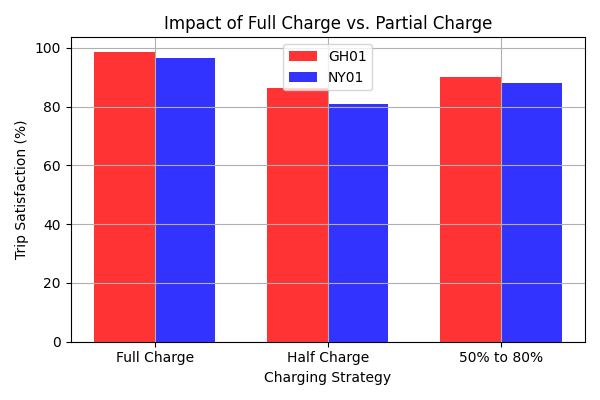
\includegraphics[scale=0.40]{Crest/Images/batery_capacitty.png}
  \caption{Impact of Charging Strategy}
  \label{fig:battery}
  \vspace{-0.1cm}
\end{figure}

These results suggest that, in general, it is more beneficial for AEVs to perform a full charge. Although full charging requires a longer stay at CSs — potentially causing AEVs to miss immediate trip opportunities — the overall system efficiency improves because vehicles can serve multiple trips consecutively without frequent interruptions for recharging.

However, this finding must be interpreted carefully in the context of the implemented \textit{eviction policy}. The eviction policy allows AEVs with higher potential (i.e., higher future trip value) to displace lower-priority AEVs from CSs. By design, eviction prevents the evicted AEVs from completing a full charge, forcing them to operate with partial battery levels.

This introduces a trade-off: while full charging is ideal for maximising the autonomy and service potential of AEVs, the eviction mechanism ensures that the most strategically important AEVs have access to charging infrastructure when needed. As a result, the system balances between:
\begin{itemize}
    \item Prioritising full charges for efficiency.
    \item Allowing strategic partial charges when necessary to maximise overall trip satisfaction.
\end{itemize}

In summary, full charging is preferable when possible, but the intelligent eviction policy ensures that the charging infrastructure remains dynamically optimised for the greater good of the entire system.

\section{Comparison with Baseline Algorithms}
\label{sec:baseline_comparison}

This section assesses the performance of the proposed charging scheduling solution approach against two baseline algorithms: First-Come, First-Served (FCFS) and Random Allocation. 

Two baselines are implemented:
\begin{itemize}
    \item \textbf{First-Come, First-Served (FCFS)}: In this algorithm, TPs are assigned to AEVs based on the order in which they arrive in the simulation. For each TP, the first available EV with enough battery and capacity is assigned to serve it.
  
    \item \textbf{Random Allocation}: In this algorithm, TPs are assigned to AEVs randomly, without considering their current battery capacity, their proximity to available CSs or their available energy.  
\end{itemize}

\subsection{FCFS Algorithm}

In Algorithm 6, the function \textit{FCFS\_Allocate} iterates over all TPs and tries to assign the first available AEV that can serve the TP. It checks for enough battery and capacity before assigning the TP.
The function\textit{ FCFS\_Charging} checks the battery levels of AEVs and sends those below a certain threshold  $\beta$  to the nearest charging station. No priority aspects are applied to the charging decisions.
\begin{algorithm}
\caption{First-Come, First-Served (FCFS) Algorithm}
\begin{algorithmic}
\Function{FCFS\_Allocate}{$T$, $E$, $Alloc$, $Sched$}
    \For{$t \in T$} \Comment{Iterate through all TPs}
        \For{$e \in E$} \Comment{Check each AEV}
            \If{$e$ can serve $t$} \Comment{AEV must have enough capacity and battery}
                \State $Alloc[t] \gets e$
                \State $Sched[e] \gets \text{update schedule with trip } t$
                \State \textbf{break}
            \EndIf
        \EndFor
    \EndFor
\EndFunction

\Function{FCFS\_Charging}{$E$, $CS$, $\beta$}
    \For{$e \in E$} \Comment{Check each AEV}
        \If{$e_{bc} \leq \beta$} \Comment{Battery below threshold}
            \State Send $e$ to nearest available charging station $cs$
        \EndIf
    \EndFor
\EndFunction
\end{algorithmic}
\end{algorithm}


\subsection{Random Allocation Algorithm}
  
In Algorithm 7, the function \textit{Random\_Allocate} randomly selects an AEV for each TP. It assigns the trip to the AEV if it has enough capacity and battery. If no suitable AEV is found, the TP is skipped.
The function \textit{Random\_Charging} sends AEVs with battery levels below the threshold  $\beta$ to a randomly selected charging station, leading to potentially inefficient energy utilisation.
\begin{algorithm}
\caption{Random Allocation Algorithm}
\begin{algorithmic}
\Function{Random\_Allocate}{$T$, $E$, $Alloc$, $Sched$}
    \For{$t \in T$} \Comment{Iterate through all TPs}
        \State $e \gets \text{Random AEV from } E$ \Comment{Randomly select an AEV}
        \If{$e$ can serve $t$} \Comment{AEV must have enough capacity and battery}
            \State $Alloc[t] \gets e$
            \State $Sched[e] \gets \text{update schedule with trip } t$
        \Else
            \State \text{Skip $t$ if no suitable AEV is available}
        \EndIf
    \EndFor
\EndFunction

\Function{Random\_Charging}{$E$, $CS$, $\beta$}
    \For{$e \in E$} \Comment{Check each AEV}
        \If{$e_{bc} \leq \beta$} \Comment{Battery below threshold}
            \State Send $e$ to a randomly selected charging station $cs$
        \EndIf
    \EndFor
\EndFunction
\end{algorithmic}
\end{algorithm}

As opposed to the two aforementioned algorithms, the proposed solution approach of Section 5.2 takes into account a variety of criteria, including trip weight, energy levels, accessibility to CSs, and future trip potential. It automatically modifies trip allocation and charging schedules to maximise trip served and energy efficiency. It includes a reward scheme in which AEVs are compensated for serving TPs from neighbouring SECs. It employs an iterative technique to fine-tuning both trip distribution and charging schedules, with the goal of achieving an optimal solution that maximises trips provided while remaining energy efficient.

The two baseline algorithms are evaluated under the same instances described in Section 5.3. The results are compared in terms of trip satisfaction, energy efficiency, and runtime performance.

\begin{enumerate}
    \item \textbf{Number of Trips Served}: This metric reflects the efficiency of the algorithms in serving TPs. A higher number of trips served indicates better service quality.

    \item \textbf{Energy Utilisation at CSs}: This metric measures how well the algorithms handle energy resources at CSs It calculates the percentage of available energy spent by AEVs when charging.

    \item \textbf{Computational Efficiency (Runtime)}: This metric measures the time taken by each algorithm to process the TPs and schedule AEVs. It reflects the scalability and computational complexity of the algorithms.
\end{enumerate}


\subsection{Analysis}
The results of the experiment are summarised in Tables \ref{tab:trips_served}, \ref{tab:energy_utilization}, and \ref{tab:runtime}. Figures \ref{fig:trips_served}, \ref{fig:energy_utilization} and \ref{fig:run_time} provide visual comparisons of the performance of the algorithms

\begin{table}[htbp]
\caption{Number of Trips Served by Each Algorithm}
\centering
\begin{tabular}{|c|c|c|c|}
\hline
\textbf{Dataset} & \textbf{Proposed Algorithm} & \textbf{FCFS} & \textbf{Random Allocation} \\
\hline
Hashcode & 98.66\% & 89.69\% & 76.34\% \\
NYC & 96.50\% & 85.23\% & 72.11\% \\
\hline
\end{tabular}
\label{tab:trips_served}
\end{table}

\begin{table}[htbp]
\caption{Energy Utilisation at CSs}
\centering
\begin{tabular}{|c|c|c|c|}
\hline
\textbf{Dataset} & \textbf{Proposed Algorithm} & \textbf{FCFS} & \textbf{Random Allocation} \\
\hline
Hashcode & 95.12\% & 83.45\% & 72.89\% \\
NYC & 94.23\% & 81.56\% & 70.34\% \\
\hline
\end{tabular}
\label{tab:energy_utilization}
\end{table}

\begin{table}[htbp]
\caption{Runtime (in Minutes) of Each Algorithm}
\centering
\begin{tabular}{|c|c|c|c|}
\hline
\textbf{Dataset} & \textbf{Proposed Algorithm} & \textbf{FCFS} & \textbf{Random Allocation} \\
\hline
Hashcode & 10 & 8 & 7 \\
NYC & 20 & 18 & 15 \\
\hline
\end{tabular}
\label{tab:runtime}
\end{table}

\begin{figure}[htbp]
\centering
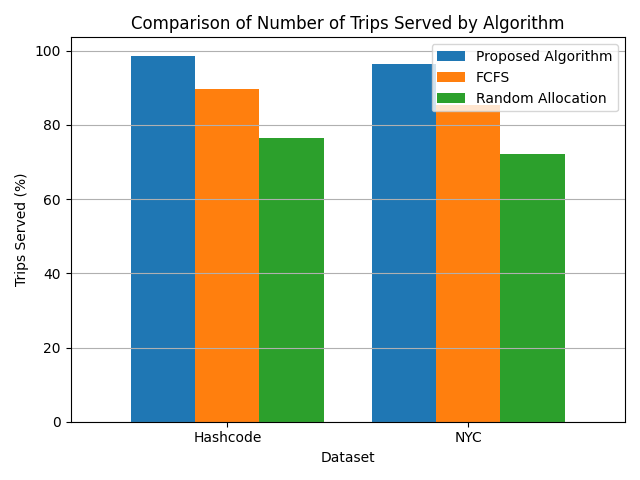
\includegraphics[scale=0.55]{Crest/Images/trips_served_comparison.png}
\caption{Number of Trips Served by Each Algorithm}
\label{fig:trips_served}
\end{figure}

\begin{figure}[htbp]
\centering
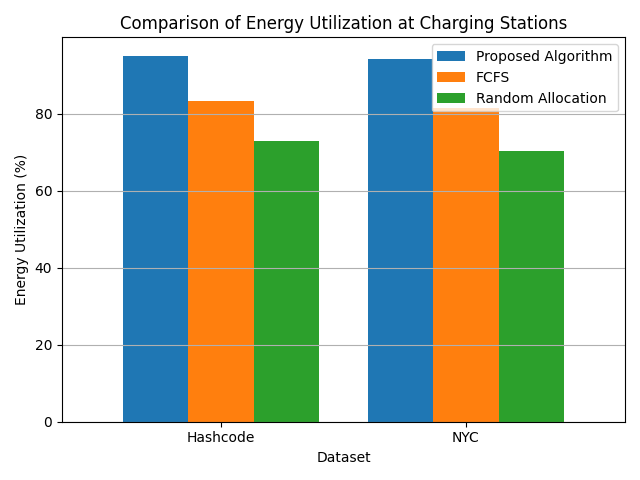
\includegraphics[scale=0.55]{Crest/Images/energy_utilization_comparison.png}
\caption{Energy Utilization at CSs}
\label{fig:energy_utilization}
\end{figure}

\begin{figure}[htbp]
\centering
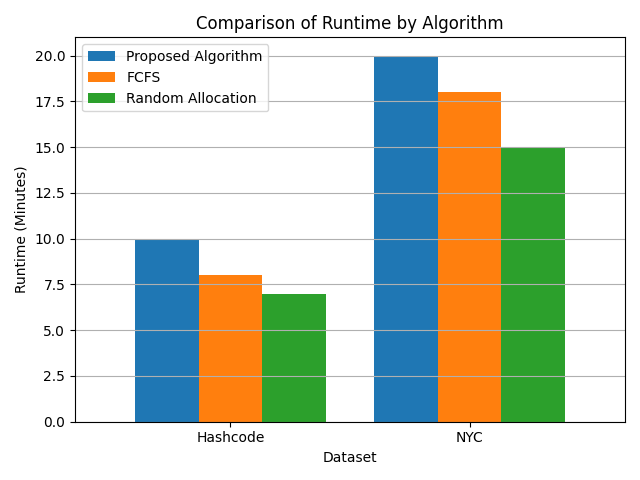
\includegraphics[scale=0.55]{Crest/Images/runtime_comparison.png}
\caption{Energy Utilization at CSs}
\label{fig:run_time}
\end{figure}

As shown in Table \ref{tab:trips_served} and Figure \ref{fig:trips_served}, the suggested method consistently outperforms both the FCFS and Random Allocation algorithms in terms of the amount of TPs being served. In the Hashcode dataset, the proposed approach served 98.66\% of TPs, while FCFS served 89.69\% and Random Allocation served just 76.34\%. A similar pattern was identified in the NYC sample.

In terms of energy utilisation (Table \ref{tab:energy_utilization} and Figure \ref{fig:energy_utilization}), the proposed algorithm demonstrated better energy management at CSs, utilising 95.12\% of available energy in the Hashcode dataset, compared to 83.45\% for FCFS and 72.89\% for Random Allocation. This pattern was consistent across both datasets.

As indicated in Table \ref{tab:runtime} and Figure \ref{fig:run_time}, the suggested method had a slightly higher runtime compared to the baseline algorithms, due to the difficulty of optimising the charging schedules and trip allocations. However, the increased runtime is offset by a large gain in trips served and energy efficiency.

\section{Impact of Charging Speed (Fast Charging vs. Slow Charging)}
\label{sec:charging_speed}

This section evaluates the performance of the ride-sharing system when different charging rates (fast vs. slow) are available at distinct charging stations. The analysis considers the number of TPs served, and the congestion at charging stations. 

Two types of charging rates are considered for the CSs:
\begin{itemize}
    \item \textbf{Fast Chargers}: High-speed charging stations,  capable of recharging AEVs at a rate of 15 kWh per unit time.
    \item \textbf{Slow Chargers}: Low-speed charging stations, capable of re-charging AEVs at a rate of 5 kWh per hour unit time.
\end{itemize}

The results are compared in terms of the following metrics:
\begin{itemize}
    \item \textbf{Number of Trips Served}: The total number of trips petitions served by the system under fast and slow charging configurations.
    \item \textbf{Average Waiting Time at Charging Stations}: The average time AEVs spend waiting to access a charging station, indicating congestion levels.
\end{itemize}

The simulation is run on the same Google HashCode and NYC instances as in section 5.4.

\subsection{Analysis}
Tables \ref{tab:trips_served_charging_speed}, \ref{tab:waiting_time}, and Figures \ref{fig:trips_served_charging_speed},  \ref{fig:waiting_time} provide the results.

\begin{table}[h]
\caption{Number of TPs Served under Different Charging Speeds}
\centering
\begin{tabular}{|c|c|c|}
\hline
\textbf{Dataset} & \textbf{50\% Fast / 50\% Slow Chargers} & \textbf{100\% Slow Chargers} \\
\hline
Google Hashcode & 98.66\% & 89.12\% \\
NYC & 96.50\% & 84.25\% \\
\hline
\end{tabular}
\label{tab:trips_served_charging_speed}
\end{table}

\begin{table}[h]
\caption{Average Waiting Time at Charging Stations (in Minutes)}
\centering
\begin{tabular}{|c|c|c|}
\hline
\textbf{Dataset} & \textbf{50\% Fast / 50\% Slow Chargers} & \textbf{100\% Slow Chargers} \\
\hline
Google Hashcode & 5.2 & 12.8 \\
NYC & 7.5 & 16.2 \\
\hline
\end{tabular}
\label{tab:waiting_time}
\end{table}

\begin{figure}[h]
\centering
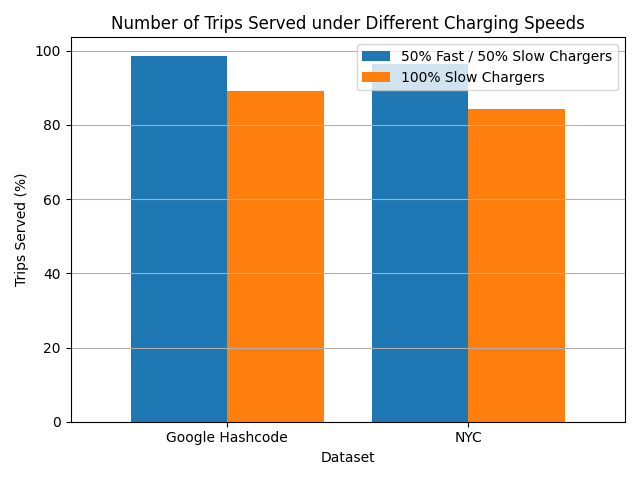
\includegraphics[scale=0.55]{Crest/Images/trips_served_charging_speed.png}
\caption{Number of Trips Served under Different Charging Speeds}
\label{fig:trips_served_charging_speed}
\end{figure}

\begin{figure}[h]
\centering
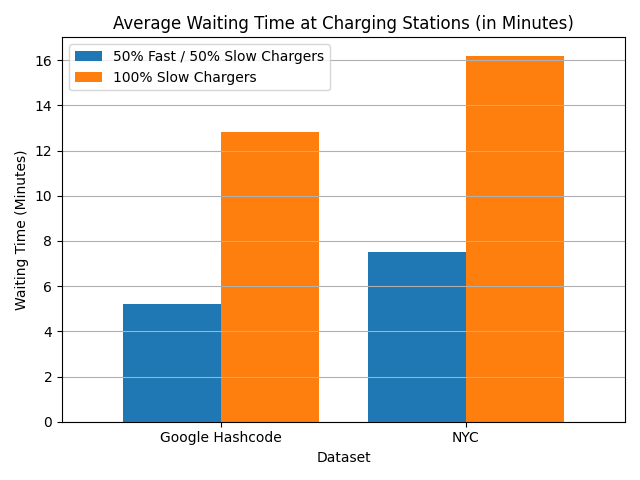
\includegraphics[scale=0.55]{Crest/Images/waiting_time_charging_speed.png}
\caption{Average Waiting Time at Charging Stations (in Minutes)}
\label{fig:waiting_time}
\end{figure}

Table \ref{tab:trips_served_charging_speed} and Figure \ref{fig:trips_served_charging_speed} indicate that using 50\% fast chargers results in considerably more trips served compared to 100\% slow chargers. In the Google Hashcode dataset, the system serves 98.66\% of TPs with fast chargers, and only 89.12\% with slow chargers. A similar tendency is seen in the NYC dataset.

Fast chargers reduce the average waiting time at charging stations significantly (Table \ref{tab:waiting_time} and Figure \ref{fig:waiting_time}). According to the Google Hashcode dataset, charging stations with 50\% fast chargers have an average waiting time of 5.2 time units, whereas 100\% slow chargers take 12.8 time units. Similar trends are seen in the NYC dataset.

\section{Impact of Renewable Energy Availability at Charging Stations}
\label{sec:renewable_energy}

This section assesses how fluctuations in availability of RES impact AEV charging schedules and overall amount of TPs being served.

The experiment models RES fluctuations at charging stations based on the following two scenarios:
\begin{itemize}
    \item \textbf{Scenario 1: Solar Power Availability} – Solar energy is available only during daytime, with energy production peaking around noon and no energy available during nighttime.
    \item \textbf{Scenario 2: Wind Energy Variability} – Wind energy fluctuates throughout the day, with varying energy availability depending on weather conditions.
\end{itemize}

The following metrics are analysed:

\begin{itemize}
    \item \textbf{Charging Station Utilisation}: The percentage of time charging stations are occupied and actively charging AEVs under varying energy availability.
    \item \textbf{Number of Trips Served}: The total number of TPs successfully served under each energy scenario.
    \item \textbf{Frequency of Charging Delays}: The number of discrete instances where AEVs experience delays in charging due to limited energy availability at CSs.
\end{itemize}

Tables \ref{tab:charging_utilization}, \ref{tab:trips_served_renewable}, and \ref{tab:charging_delays_renewable} summarize the results, and Figures \ref{fig:charging_utilization}, \ref{fig:trips_served_renewable}, and \ref{fig:charging_delays_renewable} provide visual comparisons.

\begin{table}[htbp]
\caption{Charging Station Utilisation under Different Energy Scenarios}
\centering
\begin{tabular}{|c|c|c|c|}
\hline
\textbf{Dataset} & \textbf{Baseline (Constant Energy)} & \textbf{Solar Power} & \textbf{Wind Power} \\
\hline
Google Hashcode & 85.5\% & 65.2\% & 72.1\% \\
NYC & 90.1\% & 70.3\% & 78.5\% \\
\hline
\end{tabular}
\label{tab:charging_utilization}
\end{table}

\begin{table}[htbp]
\caption{Number of Trips Served with Varying Renewable Energy Availability}
\centering
\begin{tabular}{|c|c|c|c|}
\hline
\textbf{Dataset} & \textbf{Baseline (Constant Energy)} & \textbf{Solar Power} & \textbf{Wind Power} \\
\hline
Google Hashcode & 98.66\% & 85.12\% & 90.23\% \\
NYC & 96.50\% & 82.15\% & 88.05\% \\
\hline
\end{tabular}
\label{tab:trips_served_renewable}
\end{table}

\begin{table}[htbp]
\caption{Frequency of Charging Delays under Different Energy Scenarios}
\centering
\begin{tabular}{|c|c|c|c|}
\hline
\textbf{Dataset} & \textbf{Baseline (Constant Energy)} & \textbf{Solar Power} & \textbf{Wind Power} \\
\hline
Google Hashcode & 0 & 215 & 128 \\
NYC & 0 & 425 & 240 \\
\hline
\end{tabular}
\label{tab:charging_delays_renewable}
\end{table}

Table \ref{tab:charging_utilization} and Figure \ref{fig:charging_utilization} indicate a considerable decrease in charging station use during fluctuating energy conditions. Solar electricity, which is only available during the day, yields lower utilisation than the baseline situation. Wind power, albeit variable, provides more consistent availability than solar, resulting in higher utilisation.

\begin{figure}[htbp]
\centering
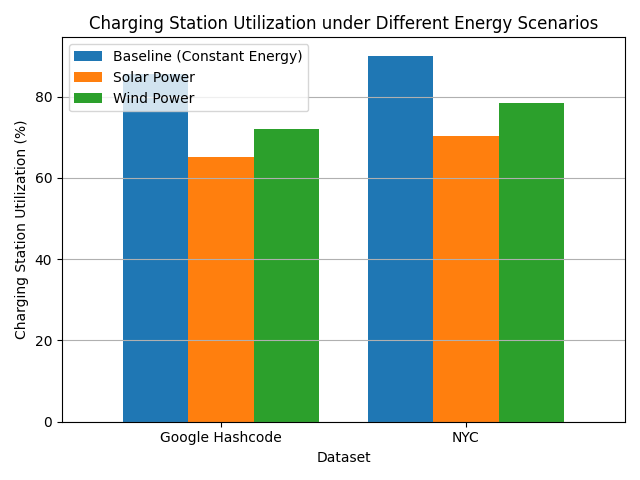
\includegraphics[scale=0.55]{Crest/Images/charging_utilization.png}
\caption{Charging Station Utilisation under Different Energy Scenarios}
\label{fig:charging_utilization}
\end{figure}

Table \ref{tab:trips_served_renewable} and Figure \ref{fig:trips_served_renewable} demonstrate that the number of trips served reduces as energy availability varies. Solar power has the highest impact, serving 85.12\% of TPs in the Google Hashcode dataset, compared to 98.66\% in the baseline. Wind power outperforms other kinds of energy due to its consistency.

\begin{figure}[htbp]
\centering
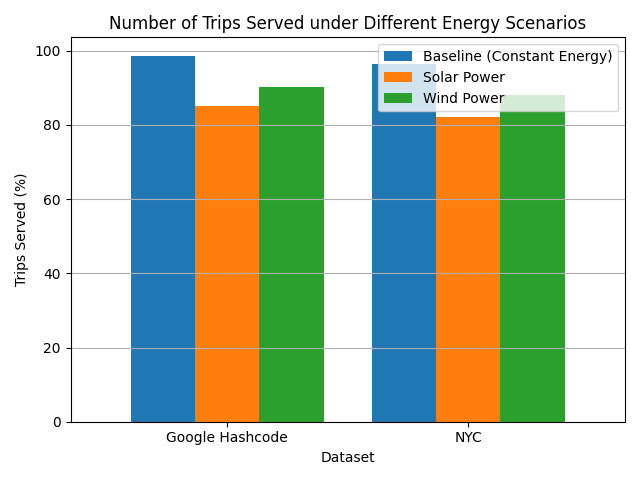
\includegraphics[scale=0.55]{Crest/Images/trips_served_renewable.png}
\caption{Number of Trips Served under Different Energy Scenarios}
\label{fig:trips_served_renewable}
\end{figure}

Table \ref{tab:charging_delays_renewable} and Figure \ref{fig:charging_delays_renewable} show that charging delays are common in both renewable energy situations. Solar electricity causes the most delays because of its limited availability at night.

\begin{figure}[htbp]
\centering
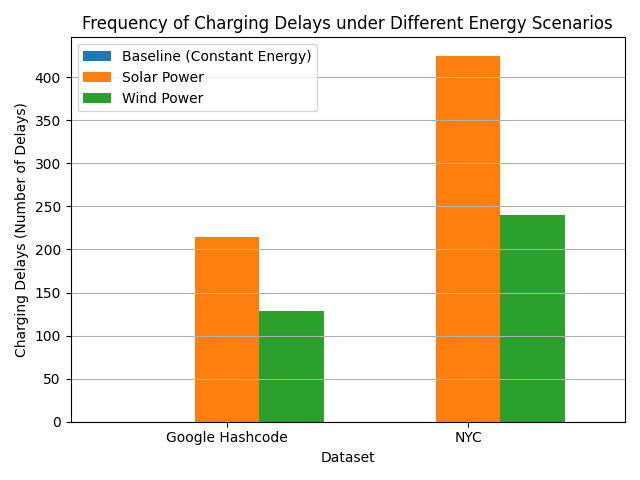
\includegraphics[scale=0.55]{Crest/Images/charging_delays_renewable.png}
\caption{Frequency of Charging Delays under Different Energy Scenarios}
\label{fig:charging_delays_renewable}
\end{figure}

The findings suggest that fluctuations in renewable energy have a major impact on the performance of the ride-sharing system. Solar energy, while sustainable, presents significant issues because to its limited availability at night, resulting in reduced charging station utilisation, fewer trips served, and longer charging delays. Wind power, while variable, provides more consistent energy supply and improves system performance. Incorporating energy storage technology or hybrid energy sources could help alleviate these effects.

\section{Impact of Varying Levels of Flexibility in TPs}
\label{sec:flexibility_trip_requests}

This section assesses how different levels of flexibility in trip pick-up and drop-off windows impact the capacity of the system to arrange trips and manage charging schedules. The relationship between flexibility and system efficiency, as well as how it affects the number of trips served, charging schedules, and energy use is examined.

The experiment simulates scenarios with varying levels of flexibility in TPs:
\begin{itemize}
    \item \textbf{Strict Flexibility}: Trips must be completed within a narrow time window, allowing minimal flexibility (e.g., 0.1 flexibility factor).
    \item \textbf{Moderate Flexibility}: Trip pick-up and drop-off windows are moderately flexible (e.g., 0.25 flexibility factor).
    \item \textbf{High Flexibility}: TPs are highly flexible, allowing significant leeway in pick-up and drop-off times (e.g., 0.5 flexibility factor).
\end{itemize}

The following key metrics are used for the evaluation:
\begin{itemize}
    \item \textbf{Percentage of Trips Served}: The proportion of TPs successfully allocated and completed under different flexibility levels.
    \item \textbf{Charging Station Utilisation}: The percentage of charging stations filled by AEVs at various levels of flexibility.
    \item \textbf{System Efficiency}: The relationship between trip flexibility and overall system efficiency, as determined by the energy consumed per trip and the total number of trips served.
\end{itemize}

% \subsection{Experimental Setup}
% The simulation is run on the following datasets:
% \begin{itemize}
%     \item \textbf{Google Hashcode Dataset}: 10,000 trip petitions and 400 AEVs.
%     \item \textbf{NYC Dataset}: 50,000 trip petitions and 1,000 AEVs.
% \end{itemize}

% Three levels of flexibility are simulated:
% \begin{enumerate}
%     \item \textbf{Strict Flexibility (5 min window)}: Very strict pick-up and drop-off time windows.
%     \item \textbf{Moderate Flexibility (15 min window)}: Moderate flexibility in time windows.
%     \item \textbf{High Flexibility (30 min window)}: High flexibility in pick-up and drop-off windows.
% \end{enumerate}

Tables \ref{tab:trips_served_flexibility}, \ref{tab:charging_utilization_flexibility}, and \ref{tab:system_efficiency_flexibility} provide a summary of the experiment output. Figures \ref{fig:trips_served_flexibility}, \ref{fig:charging_utilization_flexibility}, and \ref{fig:system_efficiency_flexibility} show visual comparisons.

\begin{table}[h]
\caption{Percentage of Trips Served under Different Flexibility Levels}
\centering
\begin{tabular}{|c|c|c|c|}
\hline
\textbf{Dataset} & \textbf{Strict} & \textbf{Moderate } & \textbf{High } \\
\hline
Google Hashcode & 78.9\% & 90.2\% & 98.1\% \\
NYC & 75.4\% & 88.5\% & 96.4\% \\
\hline
\end{tabular}
\label{tab:trips_served_flexibility}
\end{table}

\begin{table}[h]
\caption{Charging Station Utilisation under Different Flexibility Levels}
\centering
\begin{tabular}{|c|c|c|c|}
\hline
\textbf{Dataset} & \textbf{Strict} & \textbf{Moderate} & \textbf{High} \\
\hline
Google Hashcode & 72.3\% & 65.5\% & 59.8\% \\
NYC & 78.5\% & 68.7\% & 61.2\% \\
\hline
\end{tabular}
\label{tab:charging_utilization_flexibility}
\end{table}

\begin{table}[h]
\caption{System Efficiency under Different Flexibility Levels}
\centering
\begin{tabular}{|c|c|c|c|}
\hline
\textbf{Dataset} & \textbf{Strict} & \textbf{Moderate} & \textbf{High} \\
\hline
Google Hashcode & 1.5 units/trip & 1.2 units/trip & 1.0 units/trip \\
NYC & 1.6 units/trip & 1.3 units/trip & 1.1 units/trip \\
\hline
\end{tabular}
\label{tab:system_efficiency_flexibility}
\end{table}

Table \ref{tab:trips_served_flexibility} and Figure \ref{fig:trips_served_flexibility} show that as TPs become more flexible, the proportion of trips served rises. The Google Hashcode statistics shows that 98.1\% of TPs were served with high flexibility, whereas only 78.9\% were given with strict flexibility.

\begin{figure}[h]
\centering
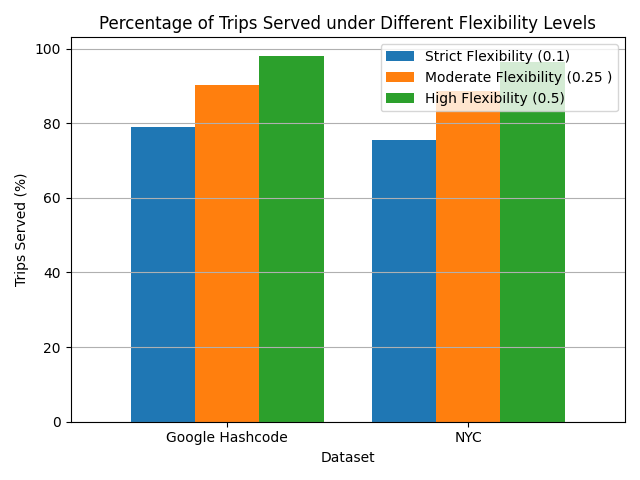
\includegraphics[scale=0.55]{Crest/Images/trips_served_flexibility.png}
\caption{Percentage of Trips Served under Different Flexibility Levels}
\label{fig:trips_served_flexibility}
\end{figure}

\begin{figure}[h]
\centering
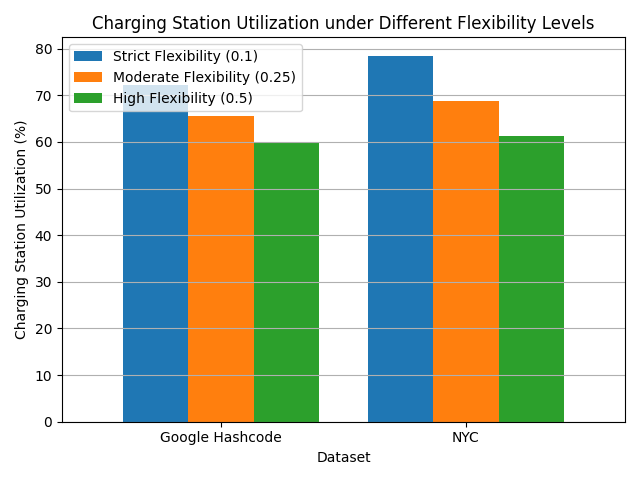
\includegraphics[scale=0.55]{Crest/Images/charging_utilization_flexibility.png}
\caption{Charging Station Utilization under Different Flexibility Levels}
\label{fig:charging_utilization_flexibility}
\end{figure}

\begin{figure}[h]
\centering
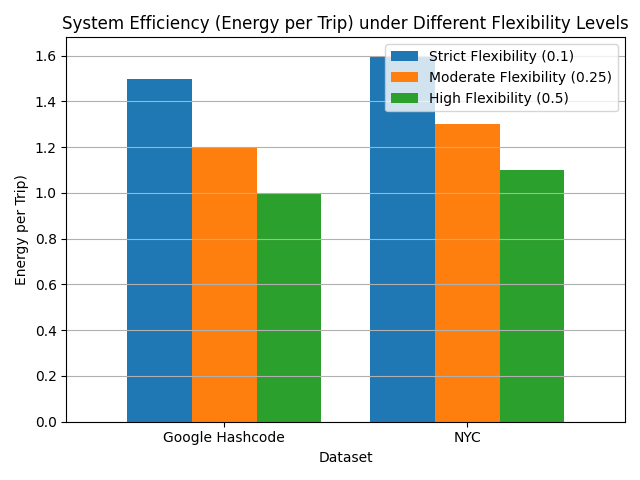
\includegraphics[scale=0.55]{Crest/Images/system_efficiency_flexibility.png}
\caption{System Efficiency (Energy per Trip) under Different Flexibility Levels}
\label{fig:system_efficiency_flexibility}
\end{figure}

Table \ref{tab:charging_utilization_flexibility} and Figure \ref{fig:charging_utilization_flexibility} show that charging station usage decreases as flexibility increases. This is because variable trip time windows enable more efficient scheduling of AEVs, resulting in less congestion at charging stations.

Table \ref{tab:system_efficiency_flexibility} and Figure \ref{fig:system_efficiency_flexibility} demonstrate that greater flexibility leads to higher system efficiency. The energy consumed per trip is lowered since AEVs may be better routed and timed with more flexible trip time slots, which results in lower energy consumption.

\section{Conclusions}
\label{sec:conclusions_and_future_work}

This chapter has presented the design, implementation, and evaluation of an reward-based, scalable charging scheduling algorithm for the carbon-neutral, community-based ride-sharing service. The model integrates multiple constraints, including energy usage, vehicle distribution, route planning, and charging station availability. The solution approach involves two key algorithms: a vehicle routing algorithm and a vehicle charging algorithm, which work in tandem to optimise the number of trips being served and energy efficiency.

The evaluation has been conducted using the same real-world datasets from Google Hashcode and NYC taxi services as per previous chapters. The proposed algorithm is designed to be flexible and adaptable to different urban environments by supporting a wide range of SECs, AEVs, TPs and CSs. 

The results demonstrate that the proposed scheduling algorithm significantly improves trip served and charging efficiency, with the system effectively handling large volumes of TPs and AEVs within a few minutes. The vehicle charging algorithm effectively meets the needs of urban transportation and sustainable energy management. By taking into account various constraints and rewards, it enhances the efficiency and reliability of the community-based ride-sharing service. The complete code can be accessed via GitHub \cite{rewardcharging}.

%As a final note, implementing a ride-sharing service that rewards users and operates without generating carbon emissions can help decrease the environmental impact of cities and encourage the adoption of sustainable transportation methods. The complete code can be accessed via GitHub \cite{rewardcharging}.
\chapter{Conclusions and Future Work}  
\label{chapter6}

This chapter presents a discussion on the findings relating to the simulation of developnig a scalable, carbon-neutral ride-sharing service based on AEVs and SECs and outlines the overall contributions of this research. It reflects on how the proposed models address current sustainability and scalability challenges and outlines directions for future research, considering the broader implications of the presented contributions to lay the groundwork for advancing the field of sustainable transportation. 

The primary objective of this thesis has been to design, implement, and evaluate a ride-sharing service model that is both scalable and carbon-neutral, leveraging the synergies between AEVs and SECs. Recognising the urgent need for sustainable mobility solutions, this work has proposed models to formalise the partition of an AEVs fleet over the SECs of a city, as well as the allocation of TPs to AEVs, their routing and charging scheduling over a simulated time horizon. These models have integrated energy generation, allocation and re-routing constraints to maximise the number of TPs served. Together, these contributions present a robust architecture for operating future community-based ride-sharing services.

Chapter 3 introduced a reactive ride-sharing service formulated as a variant of the DVRPTW. A greedy decision-making strategy, executed within a reactive simulation, maximised the number of TPs served while maintaining system responsiveness. The accompanying instance generator extended both Google Hashcode and NYC taxi datasets, enabling rigorous testing under diverse conditions. Results showed quadratic complexity in the number of trips, solving instances with 1,000 trips in under a second and 10,000 trips in under two minutes. Applied to real NYC taxi traces, the service cut fleet size by 84\% at the cost of only a 21\% increase in distance travelled, underscoring its practical scalability and environmental benefit.

Building on this foundation, Chapter 4 framed the fleet-allocation task as a decentralised, iterative negotiation among independent SECs, each competing for AEV resources to satisfy local transport demand. A Multi-Objective, Multi-Agent reinforcement-learning approach—combining Deep Q-Learning with Graph Convolutional Networks—enabled SECs to learn efficient exchange policies using only local information. Experiments on adapted Google HashCode and NYC taxi instances demonstrated near-optimal allocations when inter-SEC connectivity was high, and consistent solution quality across thousands of trips and vehicles within seconds, confirming that decentralised control can match centralised performance while better accommodating dynamic urban conditions.

Chapter 5 completed the ride-sharing service with a reward-based charging scheduler that jointly optimised the number of TPs served and energy efficiency under constraints on energy use, vehicle distribution, route plans, and charging-station availability. A two-phase algorithm—vehicle routing followed by charging optimisation—prioritised charging at times and locations with favourable RES supply or lower grid load. Tests on parameterised benchmarks confirmed that the algorithm maintained high number of TPs served and charging efficiency when working with large fleets and request volumes, therefore reinforcing the viability of the novel carbon-neutral, community-based ride-sharing service.

Taken together, these three contributions form an integrated service in which (1) reactive eco-routing delivers instant trip-matching at scale, (2) decentralised fleet negotiation balances vehicles across heterogeneous zones, and (3) incentive-aligned charging minimises carbon footprint and grid stress. The combined system scales from neighbourhood to metropolitan settings, achieves substantial reductions in private-vehicle kilometres, and operates exclusively on RES electricity—all while meeting limited real-time computational budgets. As such, the PhD thesis offers a concrete blueprint for next-generation smart-city mobility that is simultaneously sustainable, resilient, and ready for real-world deployment.

Building on these promising results, several clear opportunities exist to expand this work even further. A logical next step is to pilot the models in different operational settings, such as integrating continuous data feeds—such as real-time traffic, dynamic electricity prices, and weather forecasts—to provide more fine-grained decision-making and adaptability. 

The proposed open-source, carbon-neutral ride-sharing model can be piloted directly within MTU’s existing Park and Ride scheme \cite{mtu2024parkride}. By conceptualising surrounding neighbourhoods as SEC nodes, commuting to college will reduce the carbon footprint. Practical integration could include linking the ride-sharing app directly with MTU’s student-card and staff-ID systems to provide access and reward mechanisms, leveraging real-time data streams from campus traffic sensors and renewable-energy generation dashboards to optimise vehicle charging schedules, and establishing geo-fenced pick-up zones to reduce congestion in high-traffic areas.

Such a pilot promises substantial societal benefits. First, affordability is enhanced, as ride-sharing significantly reduces commuting expenses, which is especially important for part-time students working to cover their living costs. In addition, sustainability is improved through increased use of shared EVs, reducing the university’s transport-related carbon footprint and aligning with the EU’s Climate Action Roadmap.

Furthermore, implementing this system within MTU's operational environment would generate detailed, real-world data—including traffic patterns, energy use, user preferences, and reward responsiveness—that could be directly utilised to refine the optimisation models introduced in Chapters 3 to 5. This feedback loop would test and validate the effectiveness of the proposed algorithms under realistic, dynamic conditions such as changing schedules, variable renewable energy availability, and surges in transportation demand during examination periods. Insights gained from this pilot could guide future improvements aimed at broader urban deployment.

As battery technologies, RES infrastructures, and communication systems evolve, adapting the models to leverage new advancements, such as V2G interactions and ultra-fast charging, will be essential for maintaining long-term relevance of the service. Additionally, a comprehensive lifecycle assessment of the ride-sharing service, including manufacturing, deployment, and decommissioning phases of AEVs and SECs, would provide a holistic view of the environmental benefits of the service and of its economic feasibility. 

By addressing these challenges and opportunities, the ride-sharing service developed in this PhD thesis can be further strengthened, contributing significantly to the realisation of sustainable, smart transportation ecosystems.

While the proposed models demonstrate promising results, several limitations inherent to the current implementation should be acknowledged. First, the eviction policy applied at charging stations adopts a simplified, system-wide perspective that prioritises vehicles with higher trip-serving potential. Although effective in maximising trip petitions served, this approach overlooks possible operational constraints, such as vehicle-specific priorities, or passenger convenience, which would likely influence real-world acceptance of such policies.

Second, the simulations assume a homogeneous AEV fleet in terms of battery capacity, charging profiles, and service capability. In practice, urban fleets are diverse, comprising vehicles with varying specifications, performance characteristics, and maintenance needs. Integrating heterogeneous vehicle types would add complexity but more accurately reflect real-world operational conditions.

Finally, the models simplify the calculation of travel distances and times, using idealised or grid-based approximations to maintain computational efficiency. While suitable for large-scale algorithmic testing, this abstraction does not account for urban traffic dynamics, road network irregularities, or real-time congestion patterns. Future extensions should incorporate high-resolution, real-world transport data to enhance result realism.

These assumptions, while necessary for the current stage of development, present clear avenues for refinement and further validation, particularly in preparation for deployment in complex, real-world mobility ecosystems.



% ********************************** Bibliography ******************************
\begin{spacing}{0.9}

\bibliographystyle{abbrv}

\cleardoublepage
\bibliography{appendices/references} % Path to your References.bib file

\end{spacing}

% ********************************** Appendices ********************************
% \begin{appendices} % Using appendices environment for more functionality

% % ******************************* Thesis Appendix A ****************************
\chapter{Assessment: Ride-sharing Framrwork} 
\label{append:readiness}










% \section*{Windows OS}

% \subsection*{TeXLive package - full version}
% \begin{enumerate}
% \item	Download the TeXLive ISO (2.2GB) from\\
% \href{https://www.tug.org/texlive/}{https://www.tug.org/texlive/}
% \item	Download WinCDEmu (if you don't have a virtual drive) from \\
% \href{http://wincdemu.sysprogs.org/download/}
% {http://wincdemu.sysprogs.org/download/}
% \item	To install Windows CD Emulator follow the instructions at\\
% \href{http://wincdemu.sysprogs.org/tutorials/install/}
% {http://wincdemu.sysprogs.org/tutorials/install/}
% \item	Right click the iso and mount it using the WinCDEmu as shown in \\
% \href{http://wincdemu.sysprogs.org/tutorials/mount/}{
% http://wincdemu.sysprogs.org/tutorials/mount/}
% \item	Open your virtual drive and run setup.pl
% \end{enumerate}

% or

% \subsection*{Basic MikTeX - \TeX~ distribution}
% \begin{enumerate}
% \item	Download Basic-MiK\TeX (32bit or 64bit) from\\
% \href{http://miktex.org/download}{http://miktex.org/download}
% \item	Run the installer 
% \item	To add a new package go to Start >> All Programs >> MikTex >> Maintenance (Admin) and choose Package Manager
% \item	Select or search for packages to install
% \end{enumerate}

% \subsection*{TexStudio - \TeX~ editor}
% \begin{enumerate}
% \item	Download TexStudio from\\
% \href{http://texstudio.sourceforge.net/\#downloads}
% {http://texstudio.sourceforge.net/\#downloads} 
% \item	Run the installer
% \end{enumerate}

% \section*{Mac OS X}
% \subsection*{MacTeX - \TeX~ distribution}
% \begin{enumerate}
% \item	Download the file from\\
% \item	Extract and double click to run the installer. It does the entire configuration, sit back and relax.
% \end{enumerate}

% \subsection*{TexStudio - \TeX~ editor}
% \begin{enumerate}
% \item	Download TexStudio from\\
% \href{http://texstudio.sourceforge.net/\#downloads}
% {http://texstudio.sourceforge.net/\#downloads} 
% \item	Extract and Start
% \end{enumerate}


% \section*{Unix/Linux}
% \subsection*{TeXLive - \TeX~ distribution}
% \subsubsection*{Getting the distribution:}
% \begin{enumerate}
% \item	TexLive can be downloaded from\\
% \href{http://www.tug.org/texlive/acquire-netinstall.html}
% {http://www.tug.org/texlive/acquire-netinstall.html}.
% \item	TexLive is provided by most operating system you can use (rpm,apt-get or yum) to get TexLive distributions
% \end{enumerate}

% \subsubsection*{Installation}
% \begin{enumerate}
% \item	Mount the ISO file in the mnt directory
% \begin{verbatim}
% mount -t iso9660 -o ro,loop,noauto /your/texlive####.iso /mnt
% \end{verbatim}

% \item	Install wget on your OS (use rpm, apt-get or yum install)
% \item	Run the installer script install-tl.
% \begin{verbatim}
% 	cd /your/download/directory
% 	./install-tl
% \end{verbatim}
% \item	Enter command `i' for installation

% \item	Post-Installation configuration:\\
% \href{http://www.tug.org/texlive/doc/texlive-en/texlive-en.html\#x1-320003.4.1}
% {http://www.tug.org/texlive/doc/texlive-en/texlive-en.html\#x1-320003.4.1} 
% \item	Set the path for the directory of TexLive binaries in your .bashrc file
% \end{enumerate}

% \subsubsection*{For 32bit OS}
% For Bourne-compatible shells such as bash, and using Intel x86 GNU/Linux and a default directory setup as an example, the file to edit might be \begin{verbatim}
% edit $~/.bashrc file and add following lines
% PATH=/usr/local/texlive/2011/bin/i386-linux:$PATH; 
% export PATH 
% MANPATH=/usr/local/texlive/2011/texmf/doc/man:$MANPATH;
% export MANPATH 
% INFOPATH=/usr/local/texlive/2011/texmf/doc/info:$INFOPATH;
% export INFOPATH
% \end{verbatim}
% \subsubsection*{For 64bit OS}
% \begin{verbatim}
% edit $~/.bashrc file and add following lines
% PATH=/usr/local/texlive/2011/bin/x86_64-linux:$PATH;
% export PATH 
% MANPATH=/usr/local/texlive/2011/texmf/doc/man:$MANPATH;
% export MANPATH 
% INFOPATH=/usr/local/texlive/2011/texmf/doc/info:$INFOPATH;
% export INFOPATH

% \end{verbatim}



% %\subsection{Installing directly using Linux packages} 
% \subsubsection*{Fedora/RedHat/CentOS:}
% \begin{verbatim} 
% sudo yum install texlive 
% sudo yum install psutils 
% \end{verbatim}


% \subsubsection*{SUSE:}
% \begin{verbatim}
% sudo zypper install texlive
% \end{verbatim}


% \subsubsection*{Debian/Ubuntu:}
% \begin{verbatim} 
% sudo apt-get install texlive texlive-latex-extra 
% sudo apt-get install psutils
% \end{verbatim}


% \end{appendices}

% *************************************** Index ********************************
\printthesisindex % If index is present

\end{document}
